
\documentclass[a4paper,12pt]{report}
\usepackage{a4wide}

%\documentclass[a5paper,10pt]{book}
%\usepackage[top=23mm, bottom=18mm, left=15mm, right=25mm]{geometry}
%\geometry{papersize={170mm,220mm}}


\usepackage[utf8x]{inputenc}
\usepackage[danish]{babel}

\usepackage{xr-hyper} %Externe hyper-ref
\usepackage[colorlinks=true, hyperindex=true, linkcolor=minmblaa, citecolor=minmblaa, urlcolor=minmblaa]{hyperref}
\hypersetup{colorlinks=true,filecolor=minmblaa,bookmarksnumbered=true} %Til hyperreferencer. Referencer med farver
\usepackage{needspace} % giver mulighed for at kræve at der skal være et antal tomme linier på siden før ellers indsættes et sideskift.
\usepackage{framed} %Bokse
\usepackage{wrapfig}

\usepackage{amsmath,amsfonts,amssymb,amsthm,mathtools} %Matematikpakker

\setlength{\parindent}{0mm} %Ingen Indhak i første linje i afsnit

\usepackage{color} %Farvepakke

\usepackage{array}
\usepackage{colortbl}
\usepackage{multirow} %Til at flette rækker i tabeller.

\usepackage{verbatim,mhchem}



	% DOWNLOAD FRA: http://sarovar.org/frs/?group_id=52&release_id=97
	% Læg i directory for hoved TEX fil
%\usepackage[draft]{pdfdraftcopy}
%\draftstring{Licens: Kasper Langt Mellemnavn Skårhøj}
%\draftfontsize{30}
	%\draftfontfamily{hlh}
	%\draftangle{45}
	%\definecolor{mycolor}{rgb}{.825,.855,1}
	%\draftcolor{mycolor}
	%\draftfontattrib



% = Sidehoved =
\usepackage{fancyhdr}
\pagestyle{fancy}
\renewcommand{\sectionmark}[1]{\markright{\protect\titlegraphic{dturoed}\textcolor{dtugraa}{\thesection~\MakeUppercase{#1}}}} % \thesection.\
\fancyhead{}
\fancyfoot{}
\fancyhead[R]{\titlefont\thepage}
\fancyhead[C]{}
\fancyhead[L]{\titlefont \small eNote \MakeUppercase{~\thechapter}~\hspace*{1ex}\rightmark}
\renewcommand\headrulewidth{0pt}
\fancypagestyle{plain}{\fancyfoot[C]{}}% {\titlefont\footnotesize\thepage}}
\setlength{\headheight}{15pt}


% = Længder
%\newlength{\envtblsep}\setlength{\envtblsep}{1\FrameSep}
\newlength{\obsl}\setlength{\obsl}{\textwidth-1.2cm-13.2pt}

% Includes:

% =     Fonts (select one)    =
\usepackage{mathpazo}\linespread{1.05} % Palatino needs more leading (space between lines)
\usepackage{bm} % bold math, must be loaded after the fontpackages

% % Til overskrifter
\DeclareTextFontCommand{\th}{\fontencoding{T1}\fontfamily{phv}\fontseries{b}\selectfont}
\newcommand\titlefont{\fontencoding{T1}\fontfamily{phv}\selectfont}


% =     PGF grafik      =
\usepackage{tikz}
\newcommand\titlegraphic[1]{%
\tikz[baseline] %
\draw[thick,color=#1]
(0pt  ,-0.25em) -- (0pt  ,0.85em)
(2.5pt,-0.25em) -- (2.5pt,0.85em)
(5pt  ,-0.25em) -- (5pt  ,0.85em)
(7.5pt,-0.25em) -- (7.5pt,0.85em);\hspace*{0.8ex} %
}

\newcommand\titlegraphicwide[1]{%
\tikz[baseline] %
\draw[line width=0.8mm,color=#1]
(0pt  ,-0.25em) -- (0pt  ,0.85em)
(4.5pt,-0.25em) -- (4.5pt,0.85em)
(9pt  ,-0.25em) -- (9pt  ,0.85em)
(13.5pt,-0.25em) -- (13.5pt,0.85em);\hspace*{0.8ex} %
}


% =      Title Layout      =
\usepackage{titlesec}
\makeatletter
\titleformat{\chapter}
	[display] % Shape
	{\titlefont\Huge\flushleft} % Title and label format
	{\titlefont\LARGE\bfseries \titlegraphicwide{dturoed}\textcolor{dtugraa}{\@chapapp~\thechapter}} % label
	{0.9em} % label/title separation
	{} % before code
	[] % after code
\makeatother
\titleformat{\section}
	[hang] % Shape
	{\titlefont\Large\flushleft} % Title and label format
	{\thesection} % label
	{0.9em} % label/title separation
	{} % before code
	[] % after code
\titleformat{\subsection}
	[hang] % Shape
	{\titlefont\large} % Title and label format
	{\thesubsection} % label
	{0.9em} % label/title separation
	{} % before code
	[] % after code
\titlespacing{\subsection}{0pt}{*6}{*1.5}
\titleformat{\subsubsection}
	[hang] % Shape
	{\titlefont} % Title and label format
	{\thesubsubsection} % label
	{0.9em} % label/title separation
	{} % before code
	[] % after code



% = Farver
\definecolor{dturoed}{rgb}{0.6, 0.0, 0.0}
\definecolor{dtugraa}{rgb}{0.5, 0.5, 0.5}	% Lidt mørkere. Korrekt = 0.4
\definecolor{mingroenstreg}{rgb}{0.4,0.8,0}	% Sekundærfarve 14 : 102/204/0	(Forårsgrøn) -> Eksempler
\definecolor{mingroen}{rgb}{0.32,0.64,0}		% Sekundærfarve 14, 80% mørkere (tekst)
\definecolor{minorangestreg}{rgb}{1,0.6,0}		% Sekundærfarve 1 : 255/153/0	(Orange) -> Opgaver
\definecolor{minorange}{rgb}{0.8,0.48,0}		% Sekundærfarve 1 , 80% mørkere (tekst)

\definecolor{minblaa}{rgb}{0.2,0.4,0.8}	% Sekundærfarve 13 , 51/102/204 	( Blå -> Definitioner etc)
\definecolor{minmblaa}{rgb}{0.16,0.32,0.64}	% Sekundærfarve 13 , 80% mørkere (tekst)
\definecolor{thmbackground}{rgb}{0.97,.97, 0.99}	% Farve 13 - lys baggrund

\definecolor{mingraastreg}{rgb}{.5,.5,.5}
\definecolor{hvadbackground}{rgb}{0.97,.97, 0.97}
\definecolor{sumgul}{rgb}{1,1,.8}

\definecolor{hjmopgfarve}{rgb}{.96,1,.96}


% = Counter
\newcounter{evncount}[chapter]
\setcounter{evncount}{0}
\renewcommand{\theevncount}{\thechapter.\arabic{evncount}}
\renewcommand{\theequation}{\thechapter-\arabic{equation}}


% = Eksempler = example =
\newenvironment{example}[1][]{
	\refstepcounter{evncount}
	\setlength{\obsl}{\textwidth-1.2cm-13.2pt-9pt} % fix width of the info envirnment%
	\def\FrameCommand{ 
		\textcolor{mingroenstreg}{\vrule width 4pt} 
		\hspace{5pt} 
	}%
	\MakeFramed{\advance\hsize-\width \FrameRestore}%
	\needspace{3\baselineskip}
	\titlegraphic{mingroen}
	\textcolor{mingroen}{
		\th{Eksempel \theevncount \hspace*{5mm} #1}
	} 
	\vspace*{3mm}%
	\begin{small}
	\par
}
{
	\end{small}
	\endMakeFramed
}


% = Opgaver = exercise =
\newenvironment{exercise}[1][]{
	\refstepcounter{evncount}
	\setlength{\obsl}{\textwidth-1.2cm-13.2pt-9pt}% fix width of the info envirnment%
	\def\FrameCommand{
		\textcolor{minorangestreg}{\vrule width 4pt}
		\hspace{5pt}
	}%
	\MakeFramed{\advance\hsize-\width \FrameRestore}%
	\needspace{3\baselineskip}
	\titlegraphic{minorange}
	\textcolor{minorange}{
		\th{Opgave \theevncount \hspace*{5mm} #1}
	} 
	\vspace*{3mm}%
	\begin{small}
	\par
}
{
	\end{small}
	\endMakeFramed
}


% = Bevis
\newenvironment{bevis}{
	\setlength{\obsl}{\textwidth-1.2cm-13.2pt-9pt} % fix width of the info envirnment%
	\def\FrameCommand{
		\textcolor{mingraastreg}{\vrule width 4pt} 
		\hspace{5pt}
	}%
	\MakeFramed{\advance\hsize-\width \FrameRestore}%
	\needspace{3\baselineskip}
	\titlegraphic{black}
	\textcolor{black}{
		\th{Bevis}
	}
	\vspace*{3mm}%
	\begin{small}
	\par
}
{
	\bevisslut 
	\end{small}
	\endMakeFramed
}


% = Definition =
\newenvironment{definition}[1][]{
	\vspace{4mm}
	\pagebreak[1]
	\setlength{\obsl}{\textwidth-1.2cm-2\FrameSep-13.2pt}%
	\def\FrameCommand{
		\fboxsep=\FrameSep\fcolorbox{minblaa}{thmbackground}
	}
	\begin{minipage}{\textwidth}
	\MakeFramed{\advance\hsize-\width\FrameRestore}
	\refstepcounter{evncount}
	\titlegraphic{minblaa}
	\textcolor{minmblaa}{
		\th{Definition \theevncount \hspace*{5mm} #1}
	}
	\vspace*{3mm}
	\par
}
{
	\endMakeFramed 
	\end{minipage}
	\vspace{4mm}
}


% = Theorem =
\newenvironment{theorem}[1][]{
	\vspace{4mm}
	\pagebreak[1]%
	\setlength{\obsl}{\textwidth-1.2cm-2\FrameSep-13.2pt}%
	\def\FrameCommand{
		\fboxsep=\FrameSep\fcolorbox{minblaa}{thmbackground}
	}%
	\begin{minipage}{\textwidth}
	\MakeFramed{\advance\hsize-\width\FrameRestore}%
	\refstepcounter{evncount}
	\titlegraphic{minblaa}
	\textcolor{minmblaa}{
		\th{Sætning \theevncount \hspace*{5mm} #1}
	}
	\vspace*{3mm}
	\par
}
{
	\endMakeFramed 
	\end{minipage}
	\vspace{4mm}
}


% = Lemma =
\newenvironment{lemma}[1][]{
	\vspace{4mm}
	\pagebreak[1]
	\setlength{\obsl}{\textwidth-1.2cm-2\FrameSep-13.2pt}%
	\def\FrameCommand{
		\fboxsep=\FrameSep \fcolorbox{minblaa}{thmbackground}
	}
	\begin{minipage}{\textwidth} 
	\MakeFramed{\advance\hsize-\width \FrameRestore}
	\refstepcounter{evncount}
	\titlegraphic{minblaa}
	\textcolor{minmblaa}{
		\th{Hjælpesætning \theevncount \hspace*{5mm} #1}
	}
	\vspace*{3mm}
	\par
}
{
	\endMakeFramed 
	\end{minipage}
	\vspace{4mm}
}


% = Corollary =
\newenvironment{corollary}[1][]{
	\vspace{4mm}
	\pagebreak[1]
	\setlength{\obsl}{\textwidth-1.2cm-2\FrameSep-13.2pt}%
	\def\FrameCommand{
		\fboxsep=\FrameSep \fcolorbox{minblaa}{thmbackground}
	}
	\begin{minipage}{\textwidth} 
	\MakeFramed{\advance\hsize-\width \FrameRestore}
	\refstepcounter{evncount}
	\titlegraphic{minblaa}
	\textcolor{minmblaa}{
		\th{Følgesætning \theevncount \hspace*{5mm} #1}
	}
	\vspace*{3mm}
	\par
}
{
	\endMakeFramed 
	\end{minipage}
	\vspace{4mm}
}


% = Metode = method
\newenvironment{method}[1][]{
	\vspace{4mm}
	\pagebreak[1]
	\setlength{\obsl}{\textwidth-1.2cm-2\FrameSep-13.2pt}%
	\def\FrameCommand{
		\fboxsep=\FrameSep \fcolorbox{black}{hvadbackground}
	}
	\begin{minipage}{\textwidth} 
	\MakeFramed{\advance\hsize-\width \FrameRestore}
	\refstepcounter{evncount}
	\titlegraphic{black}
	\textcolor{black}{
		\th{Metode \theevncount \hspace*{5mm} #1}
	}
	\vspace*{3mm}
	\par
}
{
	\endMakeFramed
	\end{minipage}
	\vspace{4mm}
}


% = Forklaring = explain =
\newenvironment{explain}[1][]{
	\vspace{4mm}
	\pagebreak[1]
	\setlength{\obsl}{\textwidth-1.2cm-2\FrameSep-13.2pt}%
	\def\FrameCommand{
		\fboxsep=\FrameSep \fcolorbox{black}{hvadbackground}
	}
	\MakeFramed{\advance\hsize-\width \FrameRestore}
	\refstepcounter{evncount}
	\titlegraphic{black}
	\textcolor{black}{
		\th{Forklaring \theevncount \hspace*{5mm} #1}
	}
	\vspace*{3mm}
	\par
}
{
	\endMakeFramed
	\vspace{4mm}
}


% = Bemærkning = remark =
\newenvironment{remark}[1][]{
	\vspace{4mm}
	\pagebreak[1]
	\setlength{\obsl}{\textwidth-1.2cm-2\FrameSep-13.2pt}%
	\def\FrameCommand{
		\fboxsep=\FrameSep \fcolorbox{black}{hvadbackground}
	}
	\begin{minipage}{\textwidth} 
	\MakeFramed{\advance\hsize-\width \FrameRestore}
	\refstepcounter{evncount}
	\titlegraphic{black}
	\textcolor{black}{
		\th{Bemærkning \theevncount \hspace*{5mm} #1}
	}
	\vspace*{3mm}
	\par
}
{
	\endMakeFramed 
	\end{minipage}
	\vspace{4mm}
}







% = OBS! = obs =
\newenvironment{obs}{\vspace{4mm}\par%
\begin{tabular}{m{1.2cm}<{\hspace*{2mm}}@{}|m{\obsl}@{}}\hspace*{-4pt}\raggedleft
\includegraphics[width=1.1cm]{../Strukturfiler/FIGS/Alert01} & \begin{minipage}{\obsl}}{\end{minipage}\\ \end{tabular}\vspace{4mm}\par}


% = INFO = info =
\newenvironment{info}{\vspace{4mm}\par%
\begin{tabular}{m{1.2cm}<{\hspace*{2mm}}@{}|m{\obsl}@{}}\hspace*{-4pt}\raggedleft
\includegraphics[width=1.1cm]{../Strukturfiler/FIGS/Info01} & \begin{minipage}{\obsl}}{\end{minipage}\\ \end{tabular}\vspace{4mm}\par}


% = THINK= think =
\newenvironment{think}{\vspace{4mm}\par%
\begin{tabular}{m{1.2cm}<{\hspace*{2mm}}@{}|m{\obsl}@{}}\hspace*{-4pt}\raggedleft
\includegraphics[width=0.7cm]{../Strukturfiler/FIGS/ChessPiece} & \begin{minipage}{\obsl}}{\end{minipage}\\ \end{tabular}\vspace{4mm}\par}


% = AHA= aha =
\newenvironment{aha}{\vspace{4mm}\par%
\begin{tabular}{m{1.2cm}<{\hspace*{2mm}}@{}|m{\obsl}@{}}\hspace*{-4pt}\raggedleft
\includegraphics[width=1.1cm]{../Strukturfiler/FIGS/Think} & \begin{minipage}{\obsl}}{\end{minipage}\\ \end{tabular}\vspace{4mm}\par}


% = BUILDUP= build =
\newenvironment{build}{\vspace{4mm}\par%
\begin{tabular}{m{1.2cm}<{\hspace*{2mm}}@{}|m{\obsl}@{}}\hspace*{-4pt}\raggedleft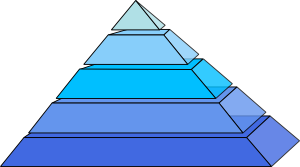
\includegraphics[width=1.1cm]{../Strukturfiler/FIGS/BluePyramid} & \begin{minipage}{\obsl}}{\end{minipage}\\ \end{tabular}\vspace{4mm}\newline}


% = Forudsætning = basis
\newenvironment{basis}{\begin{flushleft} \begin{itshape} }{\end{itshape} \end{flushleft}}


% = Opsummering =
\newenvironment{summary}{\clearpage\pagecolor{sumgul}\section{Opsummering}}{\newpage\pagecolor{white}}











% = Counter
\newcounter{opgavecount}[section]
\setcounter{opgavecount}{0}
\newcounter{spgcount}[opgavecount]
\setcounter{spgcount}{0}
\renewcommand{\thespgcount}{\alph{spgcount})}



% = EXERCISE = (DIVIDER)

\newcommand{\exercisebegin}[1][]{\bigskip\needspace{3\baselineskip}\refstepcounter{opgavecount}\titlegraphic{mingroen}\textcolor{mingroen}{\th{Opgave \theopgavecount \hspace*{1cm} #1}}\medskip\par}

% = QUIZEXERCISE = (DIVIDER)

\newcommand{\quizexercisebegin}[1][]{\bigskip\needspace{3\baselineskip}\refstepcounter{opgavecount}\titlegraphic{mingroen}\textcolor{mingroen}{\th{Quiz-Opgave \theopgavecount \hspace*{1cm} #1}}\medskip\par}

% = QUESTION =

\newenvironment{question}{\refstepcounter{spgcount}\begin{itemize}\item[\thespgcount]}{\end{itemize}\hspace*{\fill}}

% = VINK =

\newenvironment{vink}{\begin{tabular}{m{.9cm}<{\hspace*{2mm}}@{}|m{\obsl}@{}}\hspace*{-4pt}\raggedleft
\includegraphics[width=.9cm]{../Strukturfiler/FIGS/Think} & \begin{minipage}{\obsl}}{\end{minipage}\\ \end{tabular}\medskip\\}
	
% = FACIT =

\newenvironment{facit}{\begin{tabular}{m{.9cm}<{\hspace*{2mm}}@{}|m{\obsl}@{}}\hspace*{-4pt}\raggedleft
\includegraphics[width=.9cm]{../Strukturfiler/FIGS/Check} & \begin{minipage}{\obsl}}{\end{minipage}\\ \end{tabular}\medskip\\}








\newcommand{\afsnit}[1]{\bigskip\th{\titlegraphic{mingroen}\textcolor{mingroen}{#1}} \\ \rule[7pt]{.4\textwidth}{1pt} \vspace*{-2.5mm}\par}

% (DIVIDER):
\newcommand{\ugedagdatotitel}[4]{\pagebreak[4]\section{Semesteruge #1 -- #2 Dag \hspace*{1mm} (#3)} \vspace*{-4mm} \rule[5pt]{\textwidth}{1pt}\vspace*{-2.5mm} \begin{center}\large{\th{#4}}\end{center} \fancyhead[C]{\th{Semesteruge #1}}}

\newenvironment{skema}[1]{\definecolor{shadecolor}{rgb}{0.96,.98, 1.0} \setlength{\FrameSep}{6pt} \renewcommand{\FrameHeightAdjust}{10pt} \vspace*{-4pt}\begin{shaded} \begin{tabular}{#1}}{\end{tabular} \end{shaded} \vspace*{-7pt}}


% ========================

% MAKROER

%\newenvironment{matr}[1][]{\hspace*{-.8mm}\left[\hspace*{-1mm}\begin{array}{#1}}{\end{array}\hspace*{-1mm}\right]\hspace*{-.8mm}}
\newcommand{\bevisslut}{\begin{scriptsize} \begin{flushright} $ \blacksquare $ \end{flushright} \end{scriptsize}}

\newcommand{\tref}[2]{\hyperref[#1]{#2 \ref*{#1}}}
\newcommand{\thref}[2]{\hyperref[#1]{#2}}

\newcommand{\refA}[1]{\colorbox{yellow}{\ref{#1}}}
\newcommand{\hrefA}[2]{\colorbox{yellow}{\href{#1}{#2}}}
\newcommand{\trefA}[2]{\colorbox{yellow}{\hyperref[#1]{#2 \ref*{#1}}}}
\newcommand{\threfA}[2]{\colorbox{yellow}{\hyperref[#1]{#2}}}

\newenvironment{matr}[1]{\hspace*{-.8mm}\begin{bmatrix}\hspace*{-1mm}\begin{array}{#1}}{\end{array}\hspace*{-1mm}\end{bmatrix}\hspace*{-.8mm}}
\newcommand{\transp}{\hspace*{-.6mm}^{\top}}

\newcommand{\maengde}[2]{\left\lbrace \hspace*{-1mm} \begin{array}{c|c} #1 & #2 \end{array} \hspace*{-1mm} \right\rbrace}

\newenvironment{eqnalign}[1]{\setlength{\arraycolsep}{1.3pt}\begin{equation}\begin{array}{#1}}{\end{array}\end{equation}\par}
\newcommand{\eqnl}{\setlength{\arraycolsep}{1.3pt}}

\newcommand{\matind}[3]{{_\mathrm{#1}\mathbf{#2}_\mathrm{#3}}}
\newcommand{\vekind}[2]{{_\mathrm{#1}\mathbf{#2}}}
\newcommand{\jac}[2]{{\mathrm{Jacobi}_\mathbf{#1} (#2)}}
\newcommand{\diver}[2]{{\mathrm{div}\mathbf{#1} (#2)}}
\newcommand{\rot}[1]{{\mathbf{rot}\mathbf{(#1)}}}

\newcommand{\am}{\mathrm{am}}
\newcommand{\gm}{\mathrm{gm}}
\newcommand{\E}{\mathrm{E}}
\newcommand{\Span}{\mathrm{span}}
\newcommand{\mU}{\mathbf{U}}

\newcommand{\ms}{\medskip\\}
\newcommand{\bs}{\bigskip\\}

\newcommand{\mA}{\mathbf{A}}
\newcommand{\mB}{\mathbf{B}}
\newcommand{\mC}{\mathbf{C}}
\newcommand{\mD}{\mathbf{D}}
\newcommand{\mE}{\mathbf{E}}
\newcommand{\mF}{\mathbf{F}}
\newcommand{\mK}{\mathbf{K}}
\newcommand{\mI}{\mathbf{I}}
\newcommand{\mM}{\mathbf{M}}
\newcommand{\mN}{\mathbf{N}}
\newcommand{\mQ}{\mathbf{Q}}
\newcommand{\mT}{\mathbf{T}}
\newcommand{\mV}{\mathbf{V}}
\newcommand{\mW}{\mathbf{W}}
\newcommand{\mX}{\mathbf{X}}
\newcommand{\ma}{\mathbf{a}}
\newcommand{\mb}{\mathbf{b}}
\newcommand{\mc}{\mathbf{c}}
\newcommand{\md}{\mathbf{d}}
\newcommand{\me}{\mathbf{e}}
\newcommand{\mn}{\mathbf{n}}
\newcommand{\mr}{\mathbf{r}}
\newcommand{\mv}{\mathbf{v}}
\newcommand{\mw}{\mathbf{w}}
\newcommand{\mx}{\mathbf{x}}
\newcommand{\mxb}{\mathbf{x_{bet}}}
\newcommand{\my}{\mathbf{y}}
\newcommand{\mz}{\mathbf{z}}
\newcommand{\reel}{\mathbb{R}}
\newcommand{\mL}{\bm{\Lambda}} %Lambda-matrix
\newcommand{\mnul}{\bm{0}}
\newcommand{\trap}[1]{\mathrm{trap}(#1)}
\newcommand{\Det}{\operatorname{Det}}
\newcommand{\adj}{\operatorname{adj}}
\newcommand{\Ar}{\operatorname{Areal}}
\newcommand{\Vol}{\operatorname{Vol}}
\newcommand{\Rum}{\operatorname{Rum}}
\newcommand{\diag}{\operatorname{\bf{diag}}}
\newcommand{\bidiag}{\operatorname{\bf{bidiag}}}
\newcommand{\spanVec}[1]{\mathrm{span}\{#1\}}
\newcommand{\Div}{\operatorname{Div}}
\newcommand{\Rot}{\operatorname{\mathbf{Rot}}}

\newcommand{\Jac}{\operatorname{Jacobi}}
\newcommand{\Tan}{\operatorname{Tan}}
\newcommand{\Ort}{\operatorname{Ort}}
\newcommand{\Flux}{\operatorname{Flux}}
\newcommand{\Cmass}{\operatorname{Cm}}
\newcommand{\Imom}{\operatorname{Im}}
\newcommand{\Pmom}{\operatorname{Pm}}
\newcommand{\IS}{\operatorname{I}}
\newcommand{\IIS}{\operatorname{II}}
\newcommand{\IIIS}{\operatorname{III}}
\newcommand{\Le}{\operatorname{L}}
\newcommand{\app}{\operatorname{app}}
\newcommand{\M}{\operatorname{M}}
\newcommand{\re}{\mathrm{Re}}
\newcommand{\im}{\mathrm{Im}}

\newcommand{\compl}{\mathbb{C}} %de komplekse tal
\newcommand{\e}{\mathrm{e}} %eksponentialfunktionen. lodret 'e', og altså ikke kursiv ligesom andre bogstaver.





% Medialink: SCREEN: (QRcode) + thumbnail image + link på kodenummer (til qr.dtu.dk)
\newcommand{\onlinemedia}[3]{
	\begin{wrapfigure}{r}{3.2cm} 
		\vspace{-30pt} 
		\vspace{#1pt} 
		\begin{flushright} 
			\includegraphics[width=3cm]{qr/#2.png} 
			\tiny 
			\href{http://qr.dtu.dk/#2}{#2: #3}
			\normalsize  
		\end{flushright} 
		\vspace{-10pt} 
	\end{wrapfigure}
}
\newcommand{\onlinemediathumb}[3]{
	\begin{wrapfigure}{r}{3.2cm} 
		\vspace{-30pt} 
		\vspace{#1pt} 
		\begin{flushright} 
			\includegraphics[width=3cm]{qr/#2.png} 
			\includegraphics[width=3cm]{qr/#2_thumb.png} 
			\tiny 
			\href{http://qr.dtu.dk/#2}{#2: #3}
			\normalsize  
		\end{flushright} 
		\vspace{-10pt} 
	\end{wrapfigure}
}



% Index:
\usepackage{makeidx}
\makeindex
\newcommand\ind[2]{\index{#1}\textbf{\textit{\textcolor{black}{#2}}}}

% ###SERVER_EXCLUDE_BEGIN###
\externaldocument[NUID17-]{../../enoten/TN01-Talrum/Talrum}
\externaldocument[NUID1-]{../../enoten/TN02-Ligningssystemer/TNdriver}
\externaldocument[NUID2-]{../../enoten/TN03-Matricer_og_Matrixalgebra/Matricer_og_matrixalgebra}
\externaldocument[NUID3-]{../../enoten/TN04-Kvadratiske_matricer/TNdriver}
\externaldocument[NUID11-]{../../enoten/TN05-Determinanter/Determinanter}
\externaldocument[NUID12-]{../../enoten/TN06-GeometriskeVektorer/GeometriskeVektorer}
\externaldocument[NUID18-]{../../enoten/TN07-Vektorrum/VektorRum}
\externaldocument[NUID21-]{../../enoten/TN08-LinAfbildninger/LinAfbildninger}
\externaldocument[NUID23-]{../../enoten/TN09-Egenvaerdier_og_egenvektorer/TNdriver}
\externaldocument[NUID24-]{../../enoten/TN10-Diagonalisering_med_egenvektorer/TNdriver}
\externaldocument[NUID10-]{../../enoten/TN11-1.ordens_differentialligninger/TNdriver}
\externaldocument[NUID13-]{../../enoten/TN12-1.ordens_differentialligningssystemer/TNdriver}
\externaldocument[NUID14-]{../../enoten/TN13-2.ordens_differentialligninger/TNdriver}
\externaldocument[NUID27-]{../../enoten/TN14-Elemenataere_funktioner/Elementaere_Funktioner}
\externaldocument[NUID28-]{../../enoten/TN15-Funktioner2Variable/Funktioner_To_Variable}
\externaldocument[NUID29-]{../../enoten/TN16-Gradienter_og_Tangentplaner/Gradienter_og_Tangentplaner}
\externaldocument[NUID32-]{../../enoten/TN17-Taylor_formler/Taylor_Formler}
\externaldocument[NUID33-]{../../enoten/TN18-Taylor_2Var/Taylor_2Var}
\externaldocument[NUID34-]{../../enoten/TN19-SymMat/SymmetriskeMatricer}
\externaldocument[NUID35-]{../../enoten/TN20-KegleSnit/Keglesnit}
\externaldocument[NUID36-]{../../enoten/TN21-Riemann_Integral/Riemann_01}
\externaldocument[NUID37-]{../../enoten/TN22-Plan_Int/Plan_Int_01}
\externaldocument[NUID39-]{../../enoten/TN23-Flade_Int/Flade_Rum_Int_01}
\externaldocument[NUID40-]{../../enoten/TN24-Vektorfelter/Vektorfelter_01}
\externaldocument[NUID41-]{../../enoten/TN25-Flux/Flux_02}
\externaldocument[NUID42-]{../../enoten/TN26-Gauss/Gauss_01}
\externaldocument[NUID128-]{../../enoten/TN27-Stokes/Stokes_01}
\externaldocument[NUID43-]{../../enoten/TN29-KomplekseTal/KomplekseTal}

\externaldocument[NUID6-]{../../E-math-opgaver/Opgaver/opgU123}
\externaldocument[NUID19-]{../../E-math-opgaver/Opgaver/opgU45}
\externaldocument[NUID20-]{../../E-math-opgaver/Opgaver/opgU678}
\externaldocument[NUID25-]{../../E-math-opgaver/Opgaver/opgU910SD}
\externaldocument[NUID31-]{../../E-math-opgaver/OpgaverF11-U123/opgF123}
% \externaldocument[NUID9-]{../../E-math-opgaver/Opgaver/Dagsordner E10}
% ###SERVER_EXCLUDE_END###


% Begin document and set alternative chapter title:
\begin{document}
\renewcommand{\chaptername}{eNote}

\setcounter{chapter}{21} %SÆT DETTE TAL TIL 1 MINDRE END DET AKTUELLE TRANSFERNOTE-NUMMER!!

%%%%%%%%%%%%%%%%%%%%%%%%%%%%%%%%%%%%%%%%%%%%%%%%
%%%%%%%%%%%%%%%%%%%%%%%%%%%%%%%%%%%%%%%%%%%%%
%%% HERFRA SKAL DU SKRIVE ELLER INDSÆTTE %%%%
%%% DEN FIL DU ØNSKER %%%%%%%%%%%%%%%%%%%%%%%
%%%%%%%%%%%%%%%%%%%%%%%%%%%%%%%%%%%%%%%%%%%%%
%%%%%%%%%%%%%%%%%%%%%%%%%%%%%%%%%%%%%%%%%%%%%


% REF: TransferNote \ref{TN4-tn4} \nameref{TN4-tn4}
%
% \tref{NUID14-thm.koma}{sætning} \tref{NUID28-tn15}{eNote}
%
%\tref{NUID34-tn19}{eNote} Symmetriske matricer
%\tref{NUID33-tn18}{eNote} Taylor i 2 variable
%
% 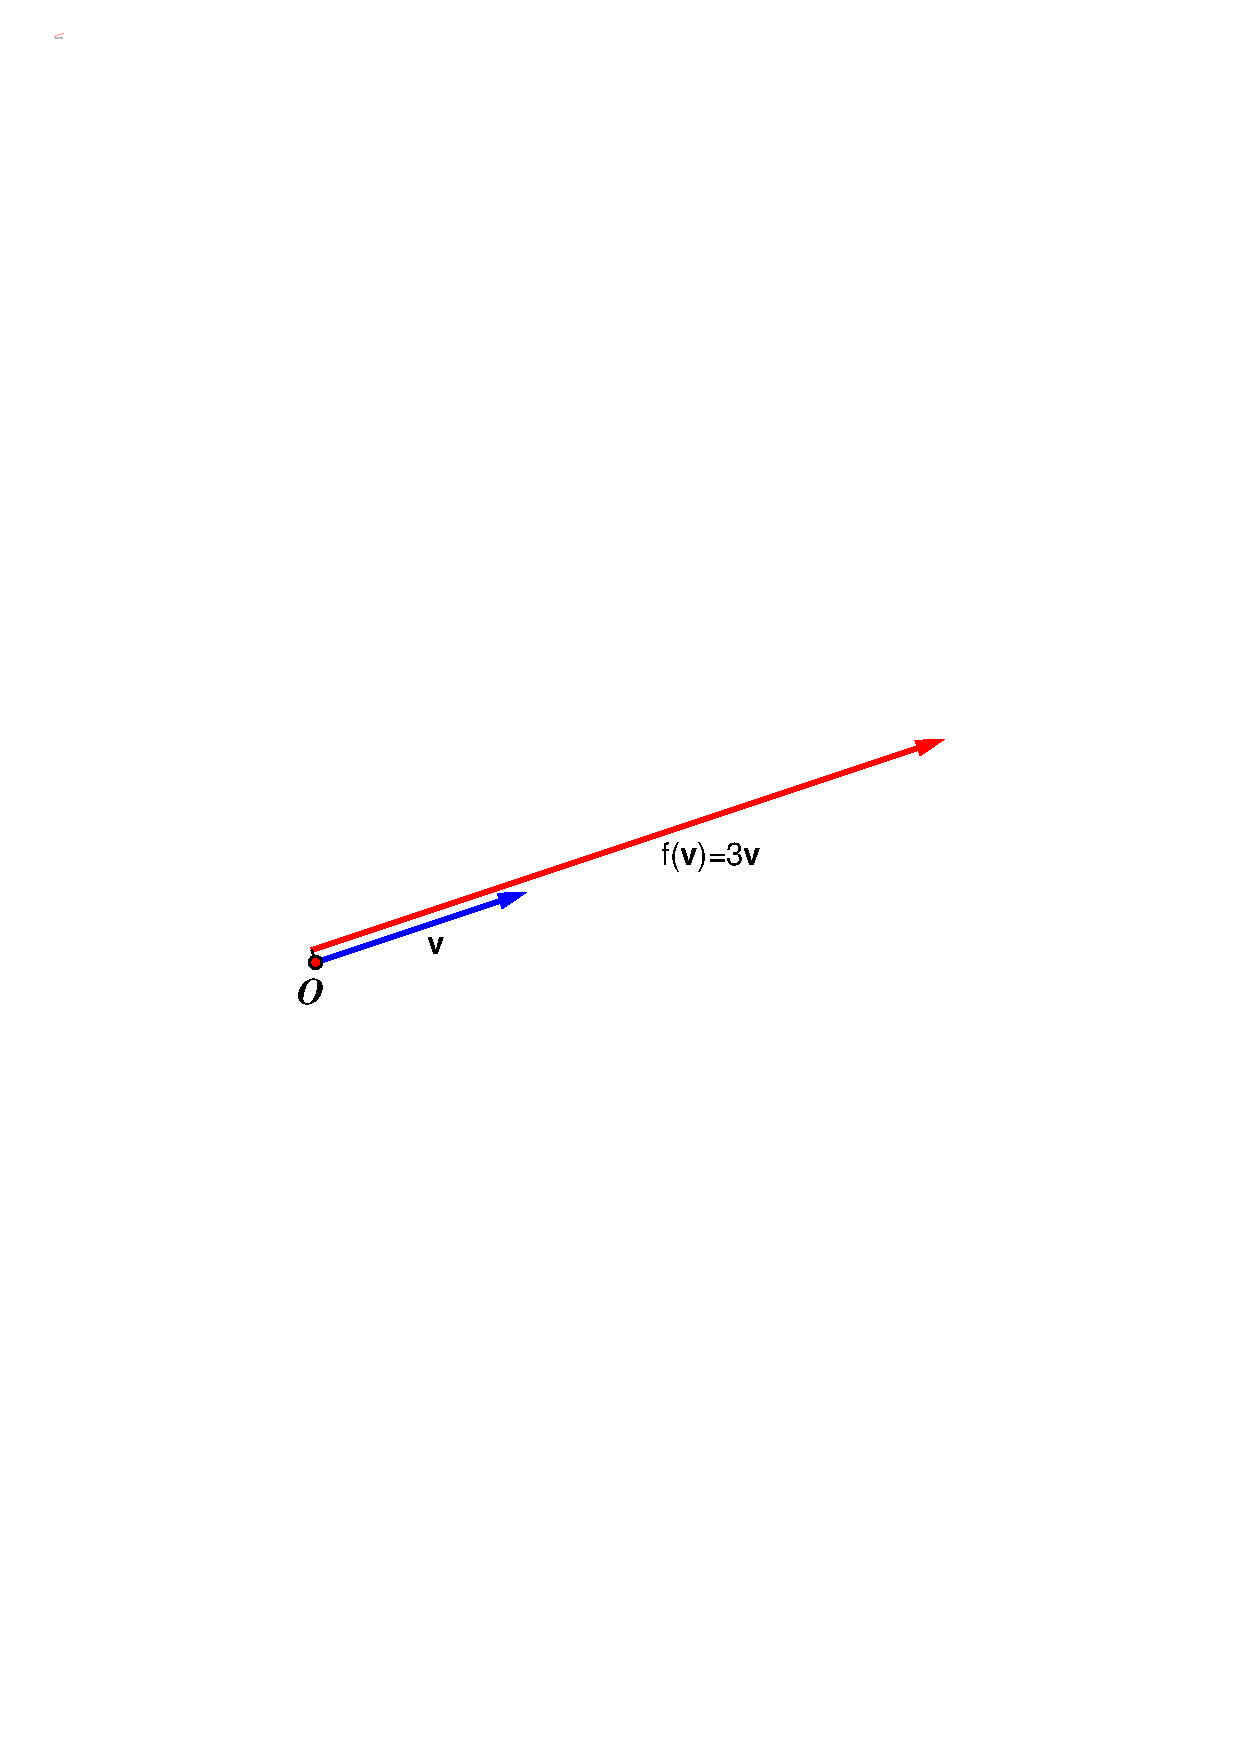
\includegraphics[trim=5cm 12cm 5cm 12cm,width=0.40\textwidth,clip]{skalering.pdf}
%
%\begin{equation}
%\matind vMa \cdot \matind aFa \cdot \matind aMv = \matind vFv \, ,
%\end{equation}
%hvor
%\begin{equation}
%\matind aMv = \begin{matr}{cccc} \vekind av_1 & \vekind av_2 & \cdots & \vekind av_n \end{matr} \quad \mathrm{og} \quad %\matind vFv = \diag(\lambda_1, \lambda_2, \ldots, \lambda_n) \, .
%\end{equation}
%
%$\vekind{e}{F}$
%$\matind{e}{F}{w}$
%
%\href{http://www-groups.dcs.st-and.ac.uk/~history/}{http://www-groups.dcs.st-and.ac.uk/~history/}

%%%%%%%%%%%%%%%%%%%%%%%%%%%%%%%%%%%%%%%%%%%%%%%%%%%
%%%%%%%%%%%%%%%%%%%%%%%%%%%%%%%%%%%%%%%%%%%%%%%%%%%
%%%%%%%%%%%%%%%%%%%%%%%%%%%%%%%%%%%%%%%%%%%%%%%%%%%
%%%%%%%%%%%%%%%%%%%%%%%%%%%%%%%%%%%%%%%%%%%%%%%%%%%

\chapter{Kurve- og plan-integraler} \label{tn22}


\begin{basis}
Vi vil her med udgangspunkt i de metoder og resultater der er opstillet i \tref{NUID36-tn21}{eNote} vise, hvordan Riemann-integralerne derfra kan benyttes til blandt andet at finde længder af kurver og  arealer af plane områder, for så vidt de er beskrevet på en passende parameterform.
\end{basis}



%%%%%%%%%%%%%%%%%%%%%%%%%%%%%%%%%%%%%%%%%%%%%%%%%%%
%%%%%%%%%%%%%%%%%%%%%%%%%%%%%%%%%%%%%%%%%%%%%%%%%%%
%%%%%%%%%%%%%%%%%%%%%%%%%%%%%%%%%%%%%%%%%%%%%%%%%%%
%%%%%%%%%%%%%%%%%%%%%%%%%%%%%%%%%%%%%%%%%%%%%%%%%%%





\section{Kurveintegraler} \label{secKurveInt}

Vi vil i udgangspunktet betragte kurver som er parametriserede på følgende måde ved
en parameterfremstilling. \\


En parametriseret kurve $K_{\bf r}$ i rummet er givet ved en
parameterfremstilling således:
\begin{equation}
\label{eqKr}
K_{\bf r}: \quad {\bf r}(u) \, = \, \left(x(u), y(u), z(u)\right)
\in \mathbb{R}^3 \quad , \, \, \,  u \in [a,b] \quad.
\end{equation}

\begin{aha}
En given kurve kan sædvanligvis parametriseres på uendelig mange måder.
Figur \ref{FigIntLine123} viser tre forskellige
parametriseringer af det rette linjestykke fra
$\, (0, -2, \frac{1}{2})\, $ til $\, (0, 2,
\frac{1}{2})\, $. Figur \ref{figc12} viser
tilsvarende to forskellige parametriseringer af
en cirkel med radius $1$ og centrum i $(0, 0,
0)$. Figur \ref{figv12} viser tilsvarende 2
forskellige parametriseringer af en skruelinje.
\end{aha}

\begin{figure}[ht]
\centerline{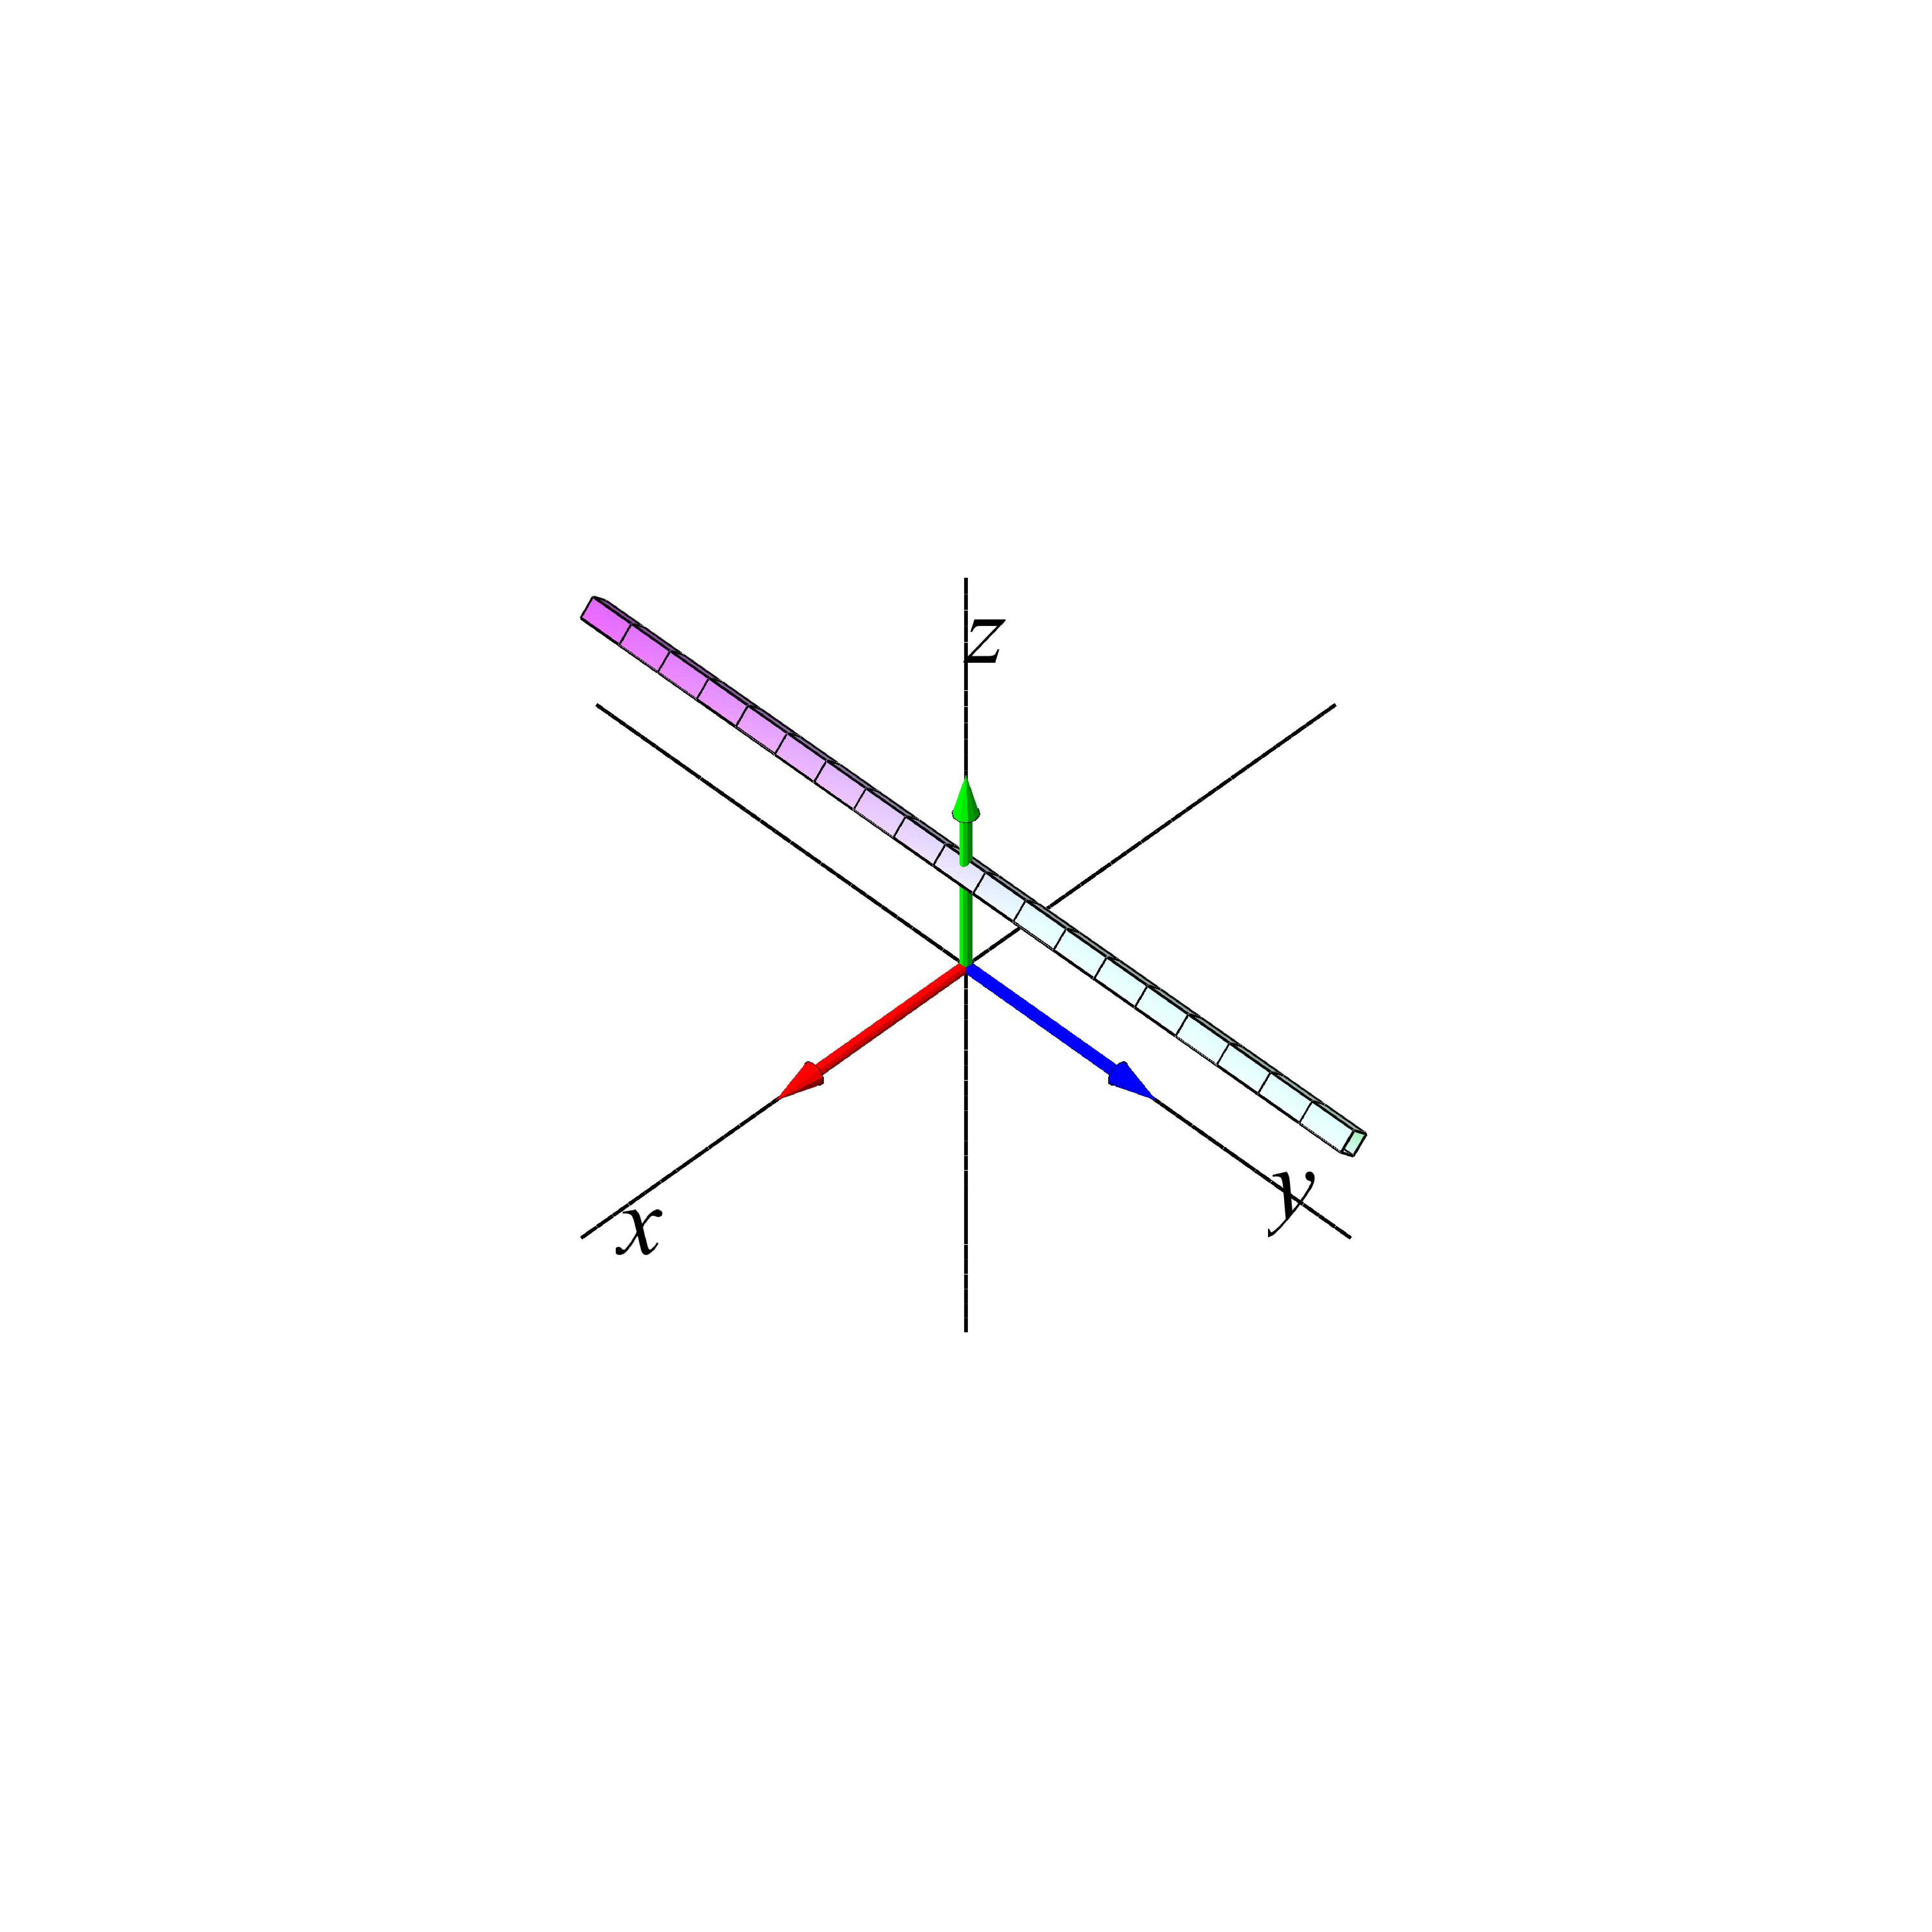
\includegraphics[height=60mm]{FIGS/plotIntLine1} 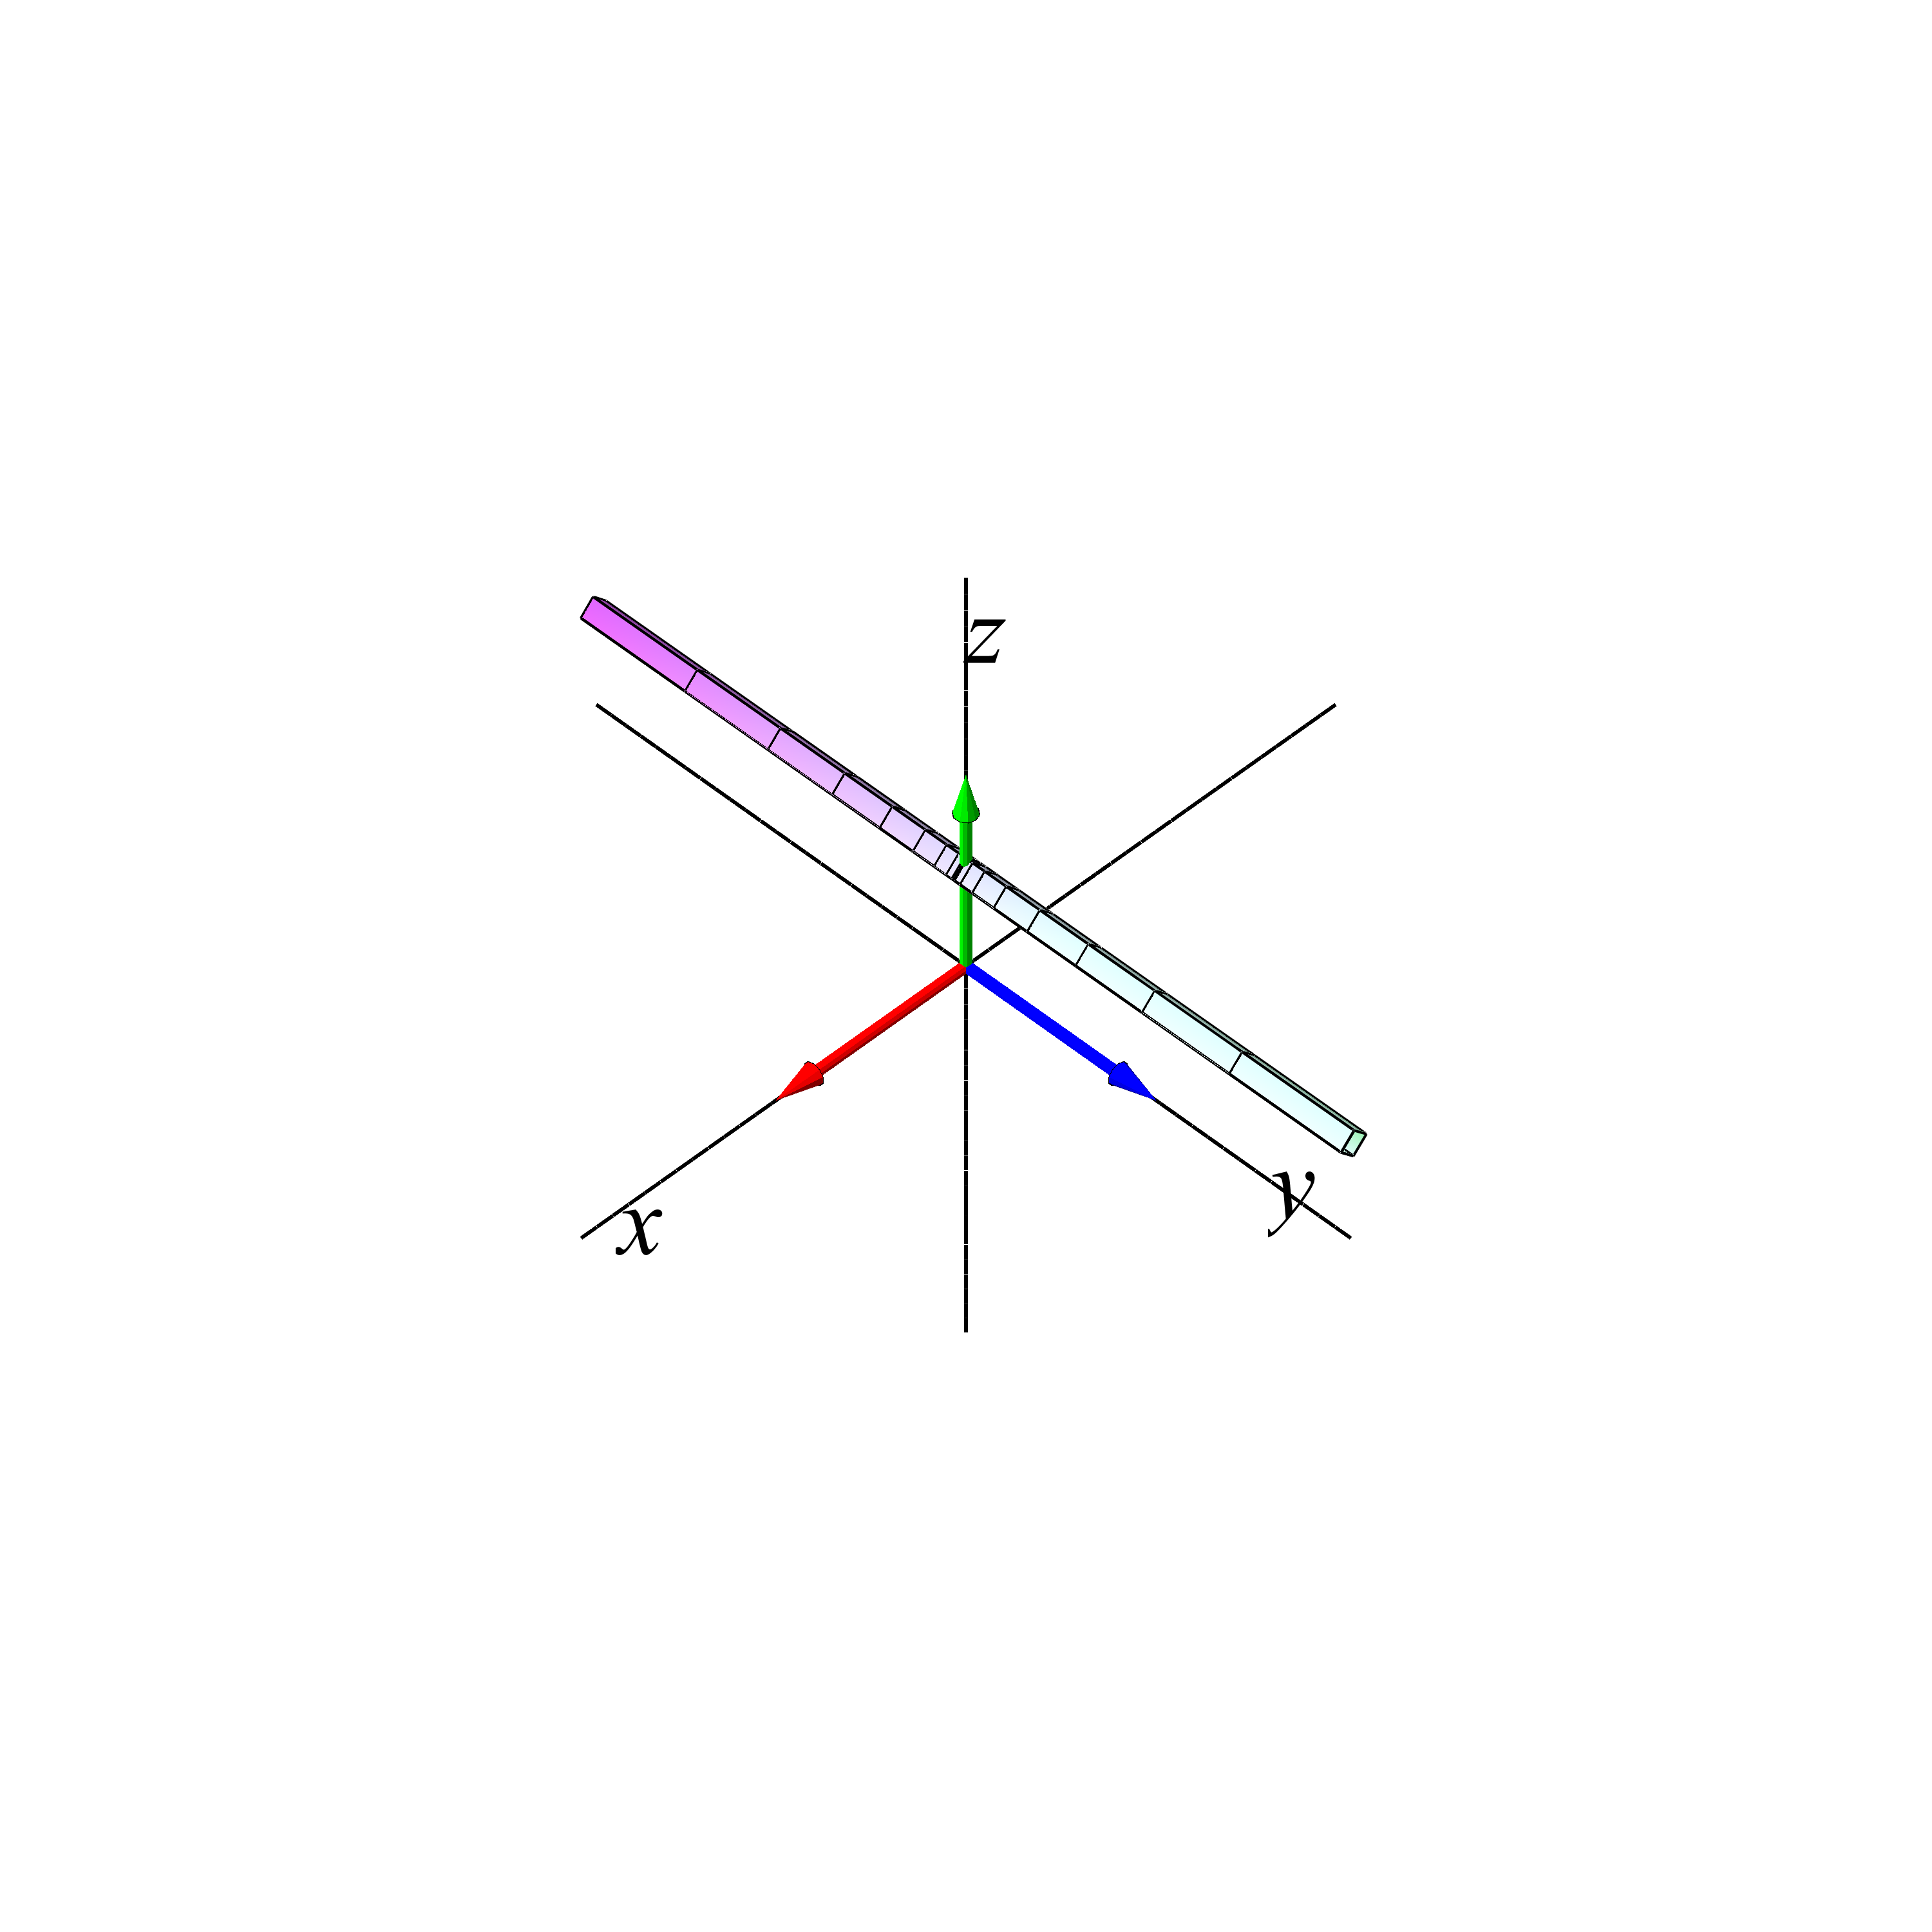
\includegraphics[height=60mm]{FIGS/plotIntLine2} 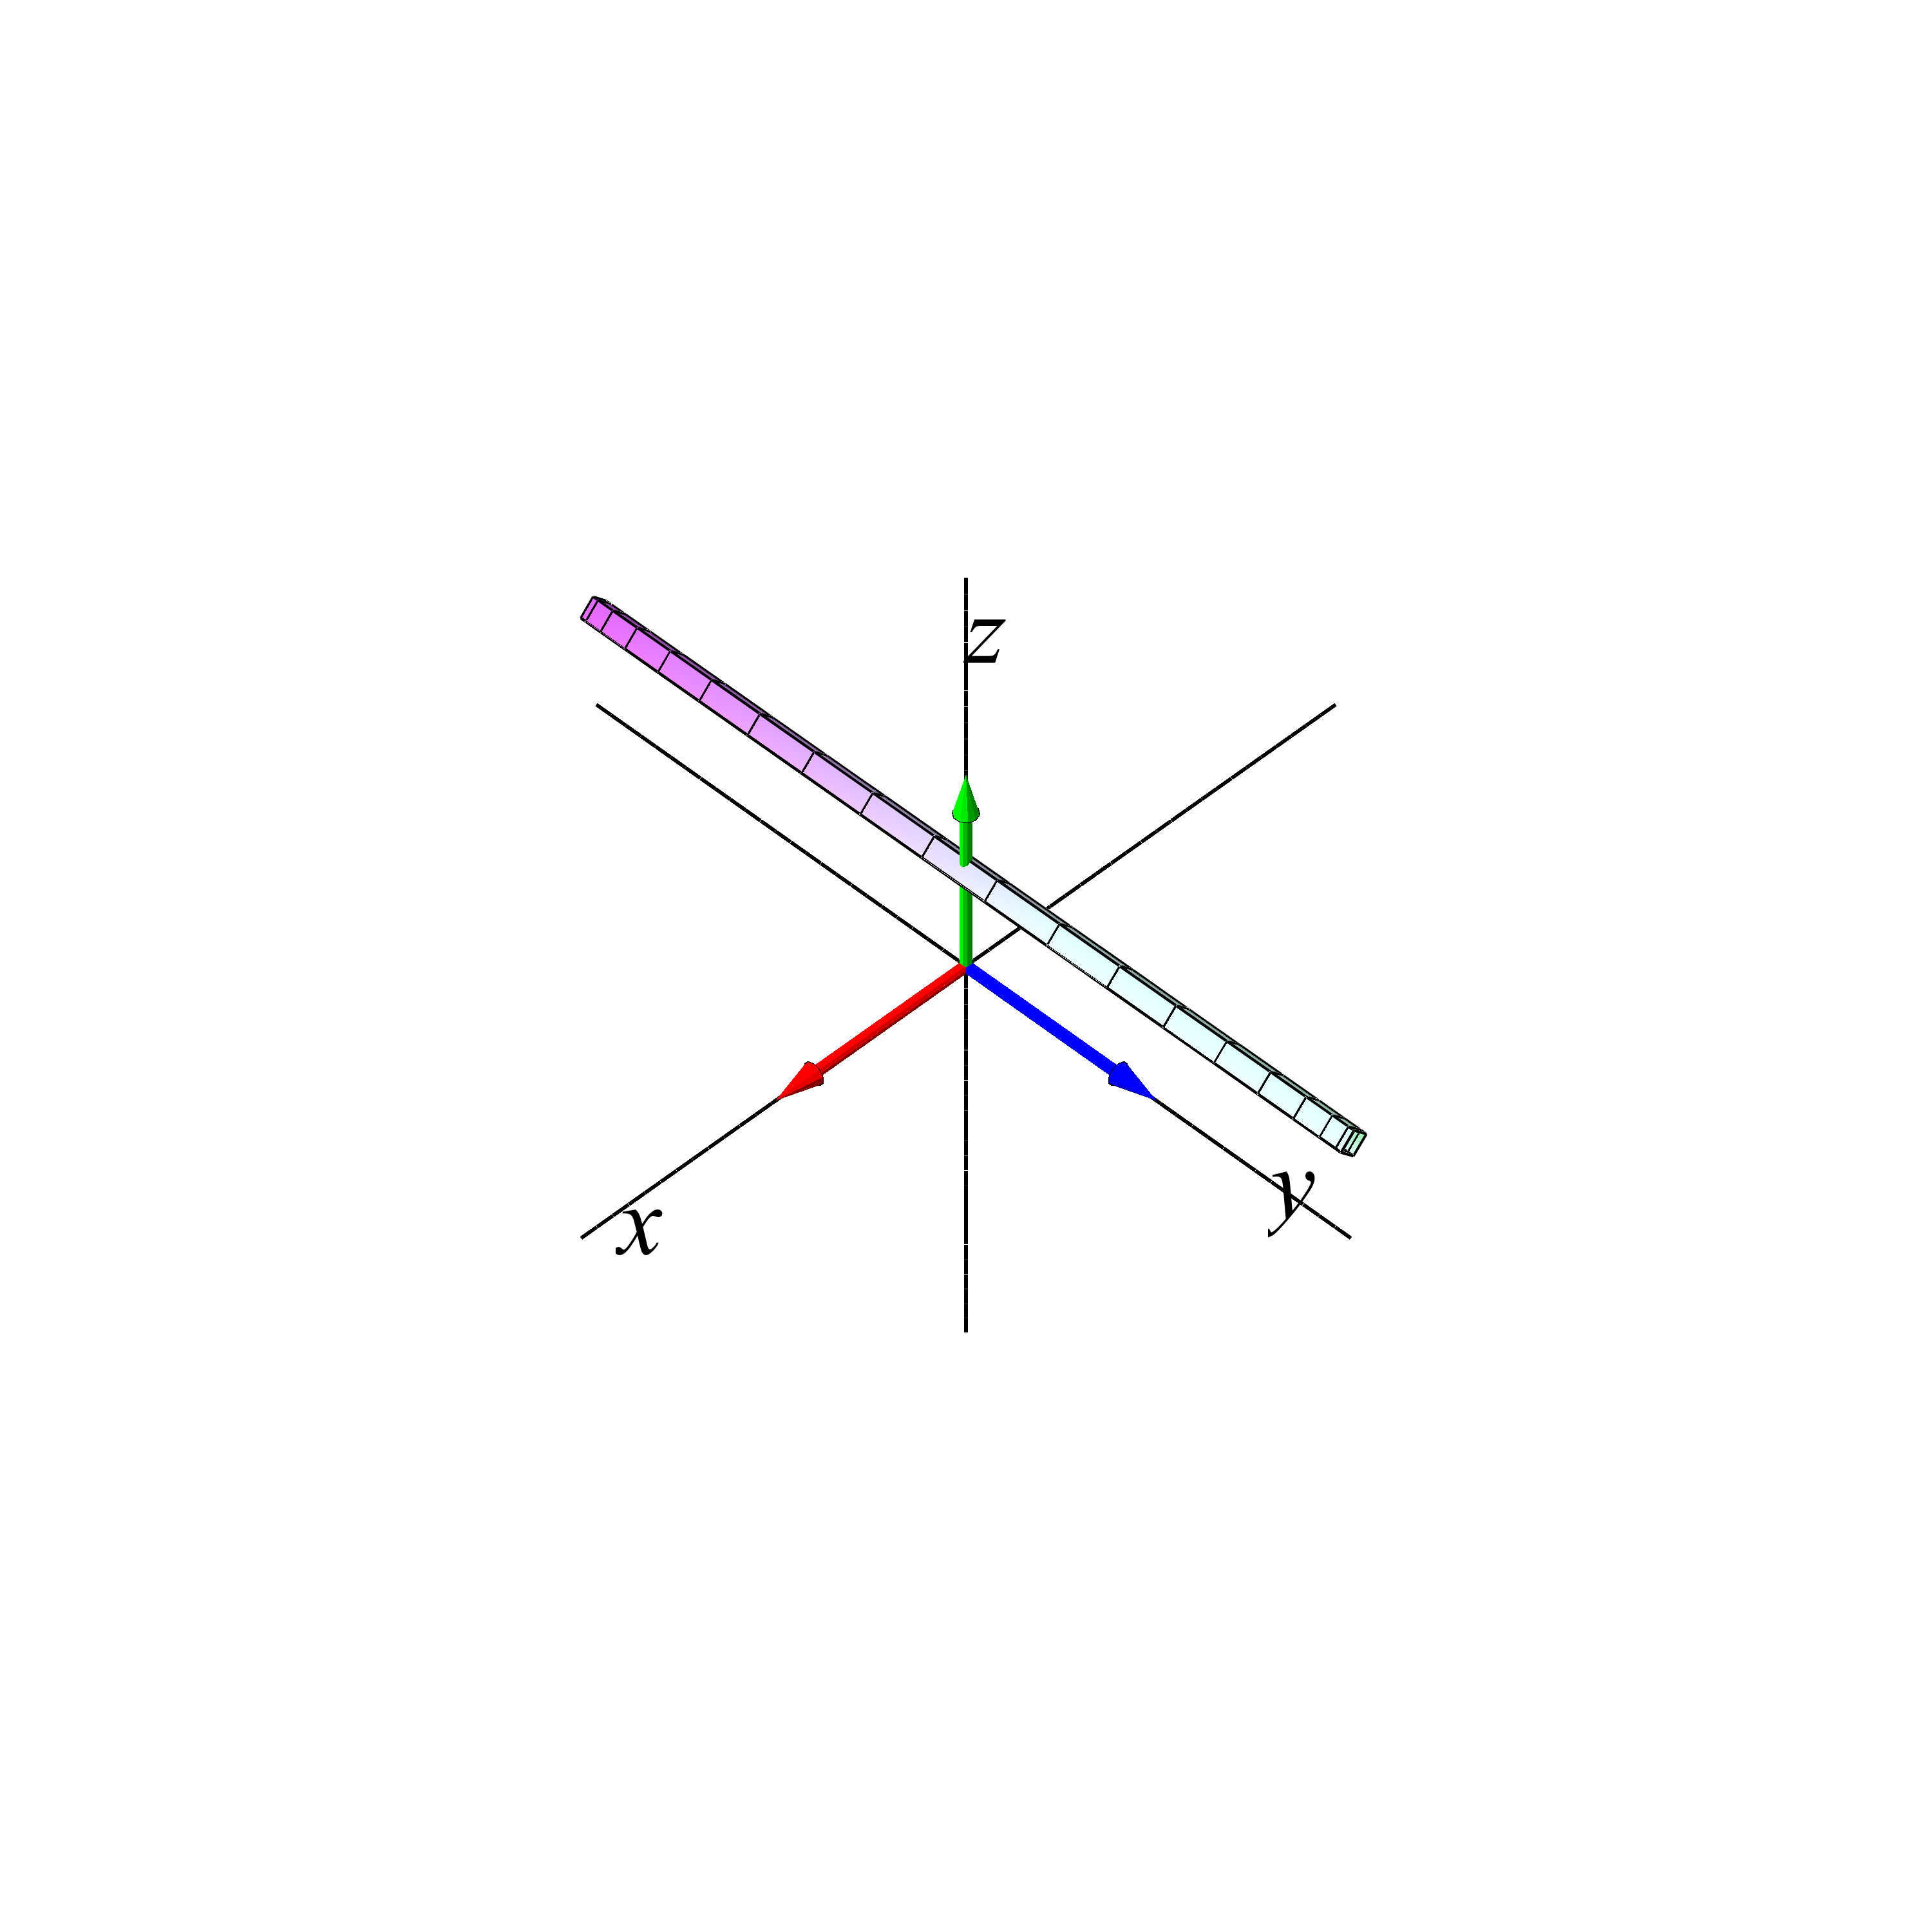
\includegraphics[height=60mm]{FIGS/plotIntLine3}}
\begin{center}
\caption{\small{Linjestykket fra $\, (0, -2,
\frac{1}{2})\, $ til $(0, \, 2, \, \frac{1}{2})$
er her parametriseret på 3 forskellige måder:
${\bf r}_{1}(u) \, = \, \left(0, 2u,
\,\frac{1}{2}\right), \, \, u \, \in [-1, \,1]\,
$; ${\bf r}_{2}(u) \, = \, \left(0, \,
2\,u^{3},\, \frac{1}{2}\right), \, \, u \, \in
[-1, 1]\, $, og ${\bf r}_{3}(u) \, = \, \left(0,
\, 2\sin(\frac{\pi}{2}u),\, \frac{1}{2}\right),
\, \, u \, \in [-1,\, 1]\, $.
Mar\-ke\-rin\-ger\-ne på de enkelte linjestykker
stammer fra den inddeling af det   {\em fælles
parameterinterval $\, [-1,\, 1]\,$} som består af
$20$ lige store delintervaller. Bemærk, at
længden af de tre 'kurver' klart er den samme,
selv om parametriseringerne er ret forskellige. Se Opgave \ref{exercLaengde}.}}
\label{FigIntLine123}
\end{center}
\end{figure}



Vi antager her og i det følgende, at de tre
koordinatfunktioner $x(u)$, $y(u)$ og $z(u)$ i
{parameterfremstilling}erne er pæne funktioner af
$u$. Vi antager simpelthen, at de alle tre er glatte funktioner af $u$ således at de kan
differentieres vilkårligt mange gange. Specielt er de afledede funktioner $x'(u)$,
$y'(u)$ og $z'(u)$
derfor kontinuerte i intervallet $[a,b]$. Så har
vi også, at
\begin{equation}  | {\bf r}'(u) |  \, =
\, \sqrt{x'(u)^{2} + y'(u)^{2} + z'(u)^{2}}
\end{equation}
er en kontinuert funktion i intervallet $[a, b]$. Specielt
kan denne funktion derfor {\em integreres} over intervallet, jvf. \tref{NUID36-tn21}{eNote}  og
det har vi om lidt  brug for i definition \ref{defKurveInt}
nedenfor.

\begin{definition}[Regulær parameterfremstilling] \label{defRegKurve}
En parameterfremstilling ${\bf r}(u)$ for en kurve $K_{\bf r}$ -
som i (\ref{eqKr}) - siges at være en {\em{{regulær parameterfremstilling}}} hvis
følgende betingelse er opfyldt:
\begin{equation}
{\bf r}'(u) \neq {\bf 0} \quad \text{for alle} \quad  u \in [a, b] \quad .
\end{equation}
\end{definition}

\begin{exercise}
Hvilke af parameterfremstillingerne i figurerne \ref{FigIntLine123},
\ref{figc12}, \ref{figv12}, og \ref{figKnude} er regulære?
\end{exercise}


\begin{think}
En parametriseret kurve er andet og mere end blot billedmængden
(punktmængden) ${\bf r}([a, b ])$, idet selve parametriseringen
eksempelvis kan foreskrive at dele af punktmængden skal gennemløbes
flere gange, se eksempel \ref{exKurveLang} nedenfor.\\

Man kan gerne tænke på intervallet $[a, b ]$ som en retlinet elastik
i hvile. Vektor-afbildningen ${\bf r}$ deformerer elastikken (ind i
rummet) ved at bøje, strække eller komprimere elastikken. En lokal
strækning gør selvfølgelig elastikken lokalt længere, mens en lokal
komprimering gør elastikken lokalt kortere. Et første naturligt
spørgsmål er derfor hvor lang hele elastikken er efter brug af
afbildningen ${\bf r}$. Kurveintegralet indføres blandt andet med
henblik på at finde den totale længde af den deformerede kurve i
rummet. \\

Vi kan ligeledes forestille os, at den parametriserede kurve selv er
masseløs, men at den til gengæld efter deformationen med ${\bf r}$
farves med en maling på en sådan måde at massetætheden af malingen
langs med kurven (i gram pr. centimeter, f.eks.) er givet som en
funktion $f$ af stedet $(x, y, z)$ i rummet -- altså sådan at
massetætheden af malingen på stedet ${\bf r}(u)$ er $f({\bf r}(u))$.
Opgaven er da at finde den totale masse af den deformerede og
farvelagte parametriserede kurve. Bemærk, at med lidt fantasi kan vi
endda gerne tillade, at 'massetætheden'  $f$ antager negative
værdier. \\

Disse forestillinger skal naturligvis kun hjælpe os til at få en passende
intuitiv forståelse af de indførte begreber; vi skal i de relaterede eNoter
se adskillige andre tolkninger og brug af kurveintegralet.

\end{think}




\begin{figure}[ht]
\centerline{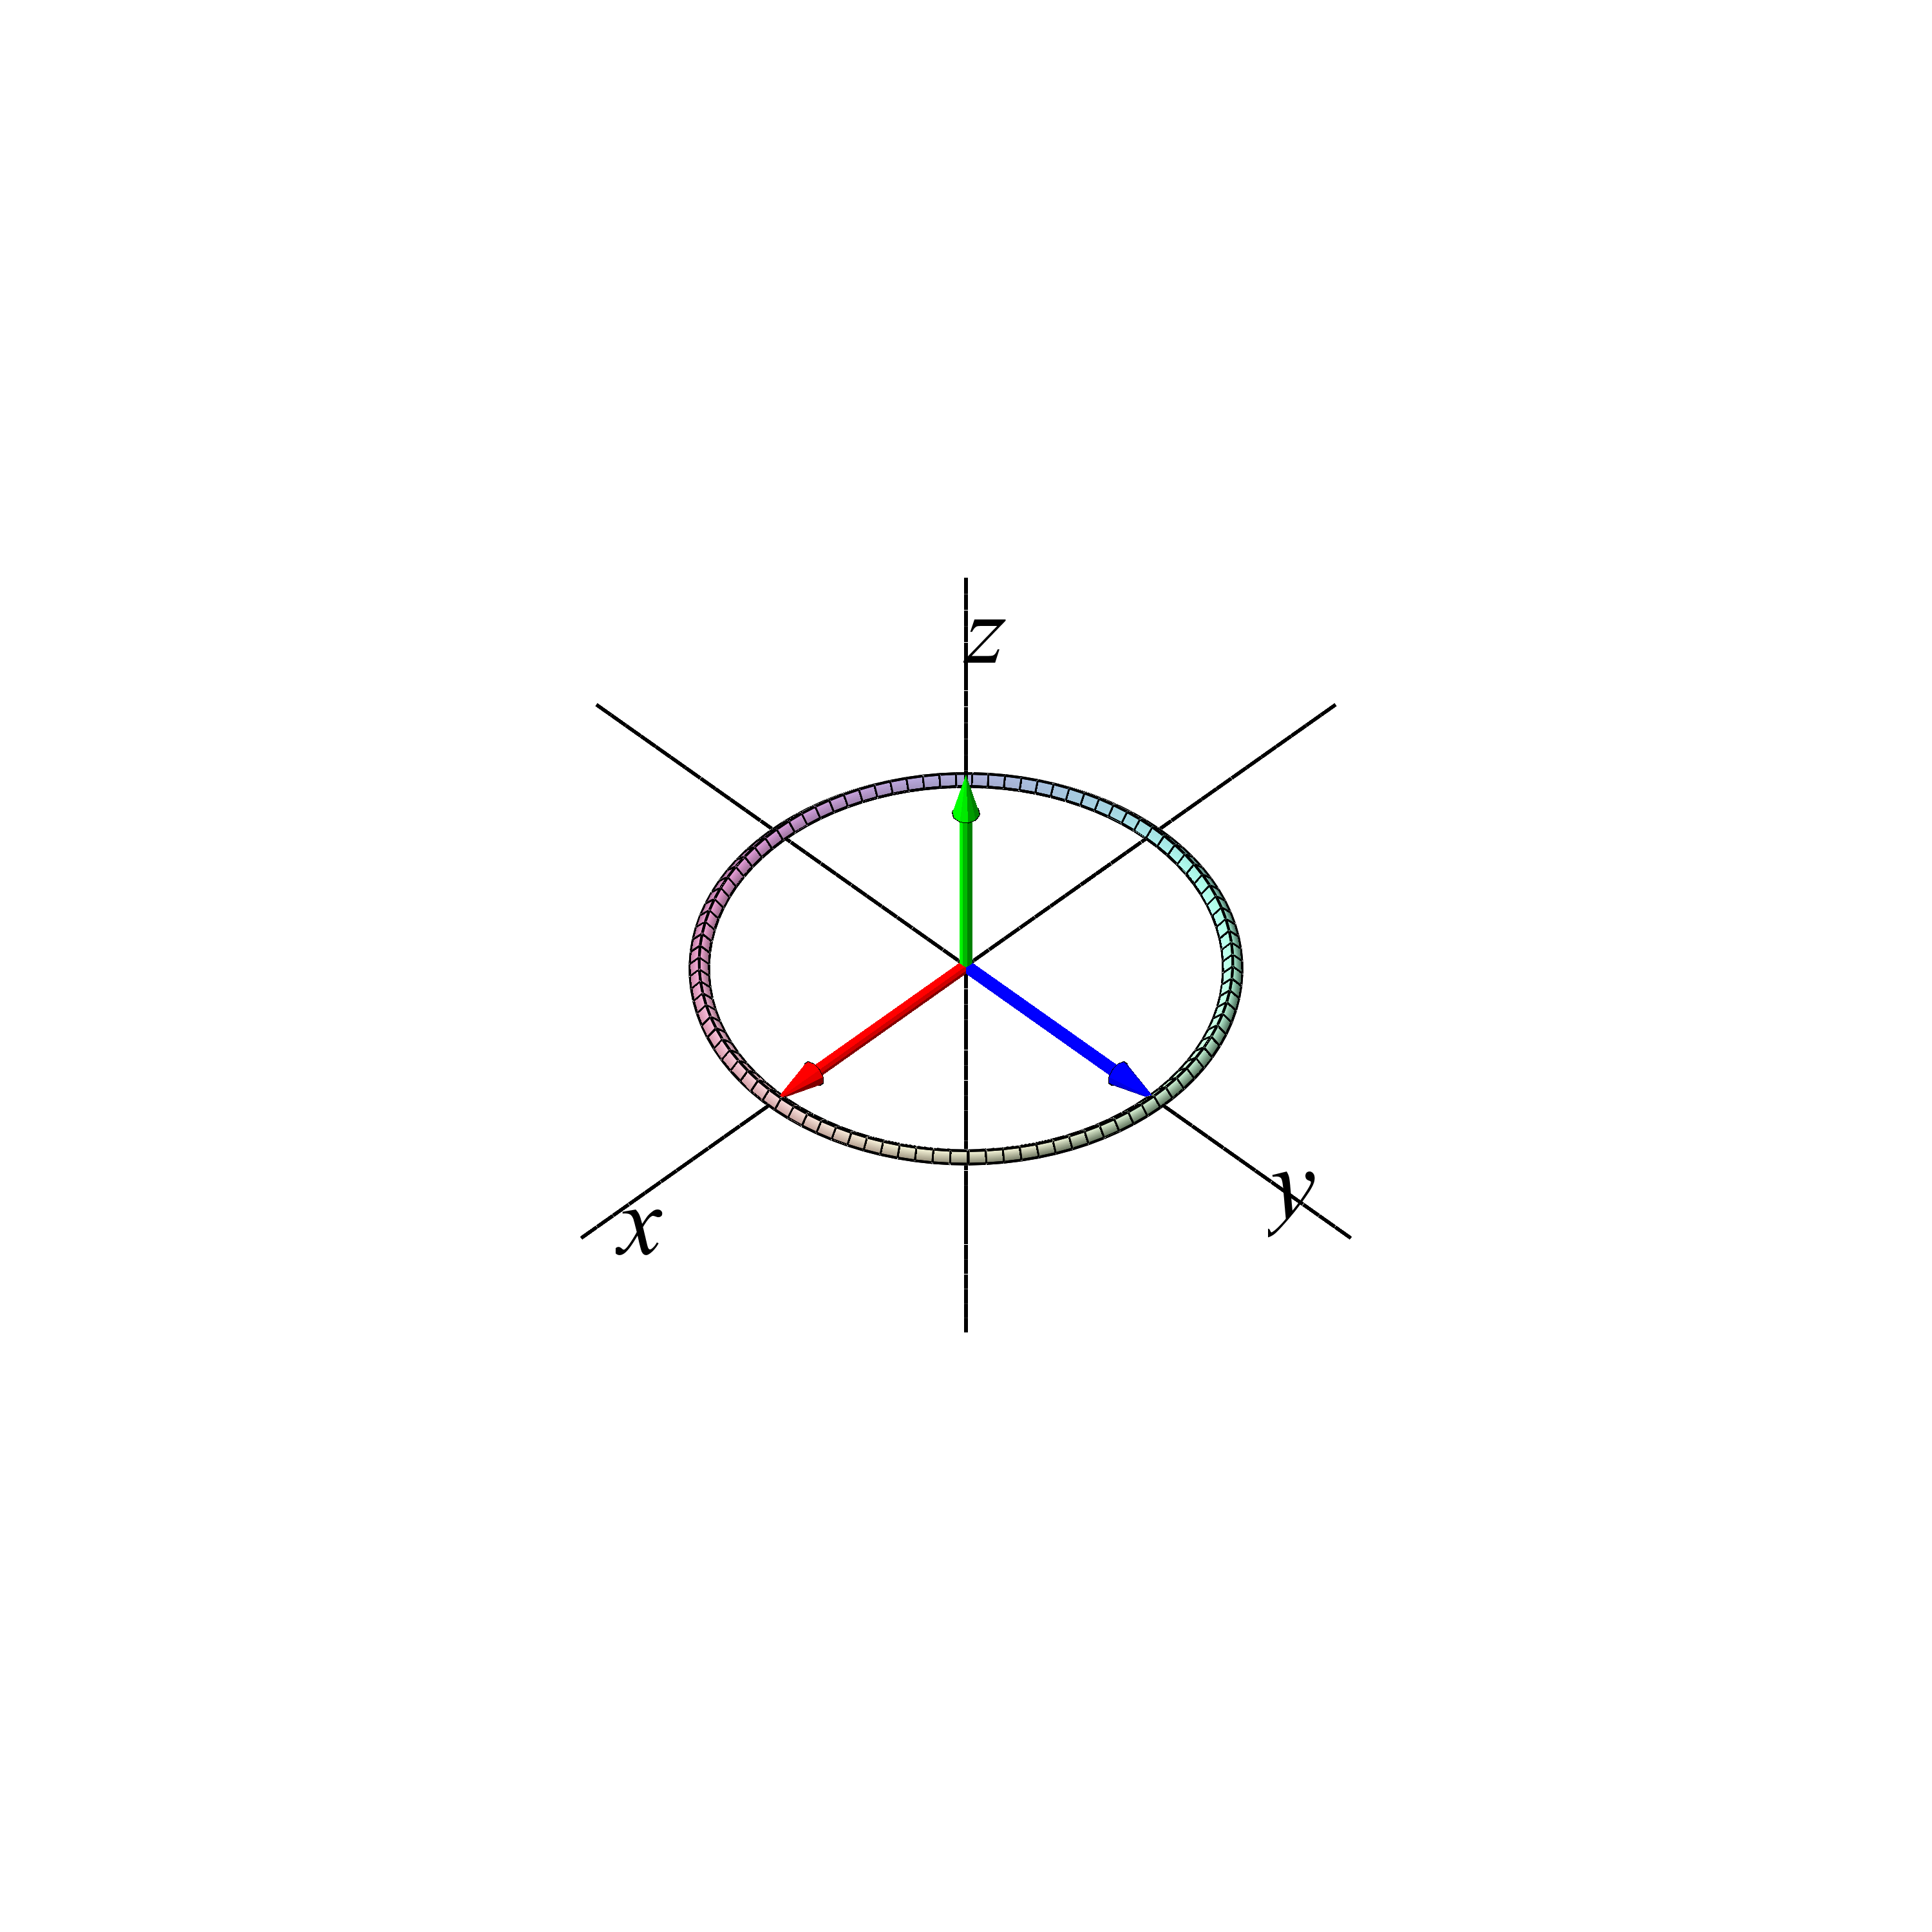
\includegraphics[height=80mm]{FIGS/plotC1}\, \, \, \quad  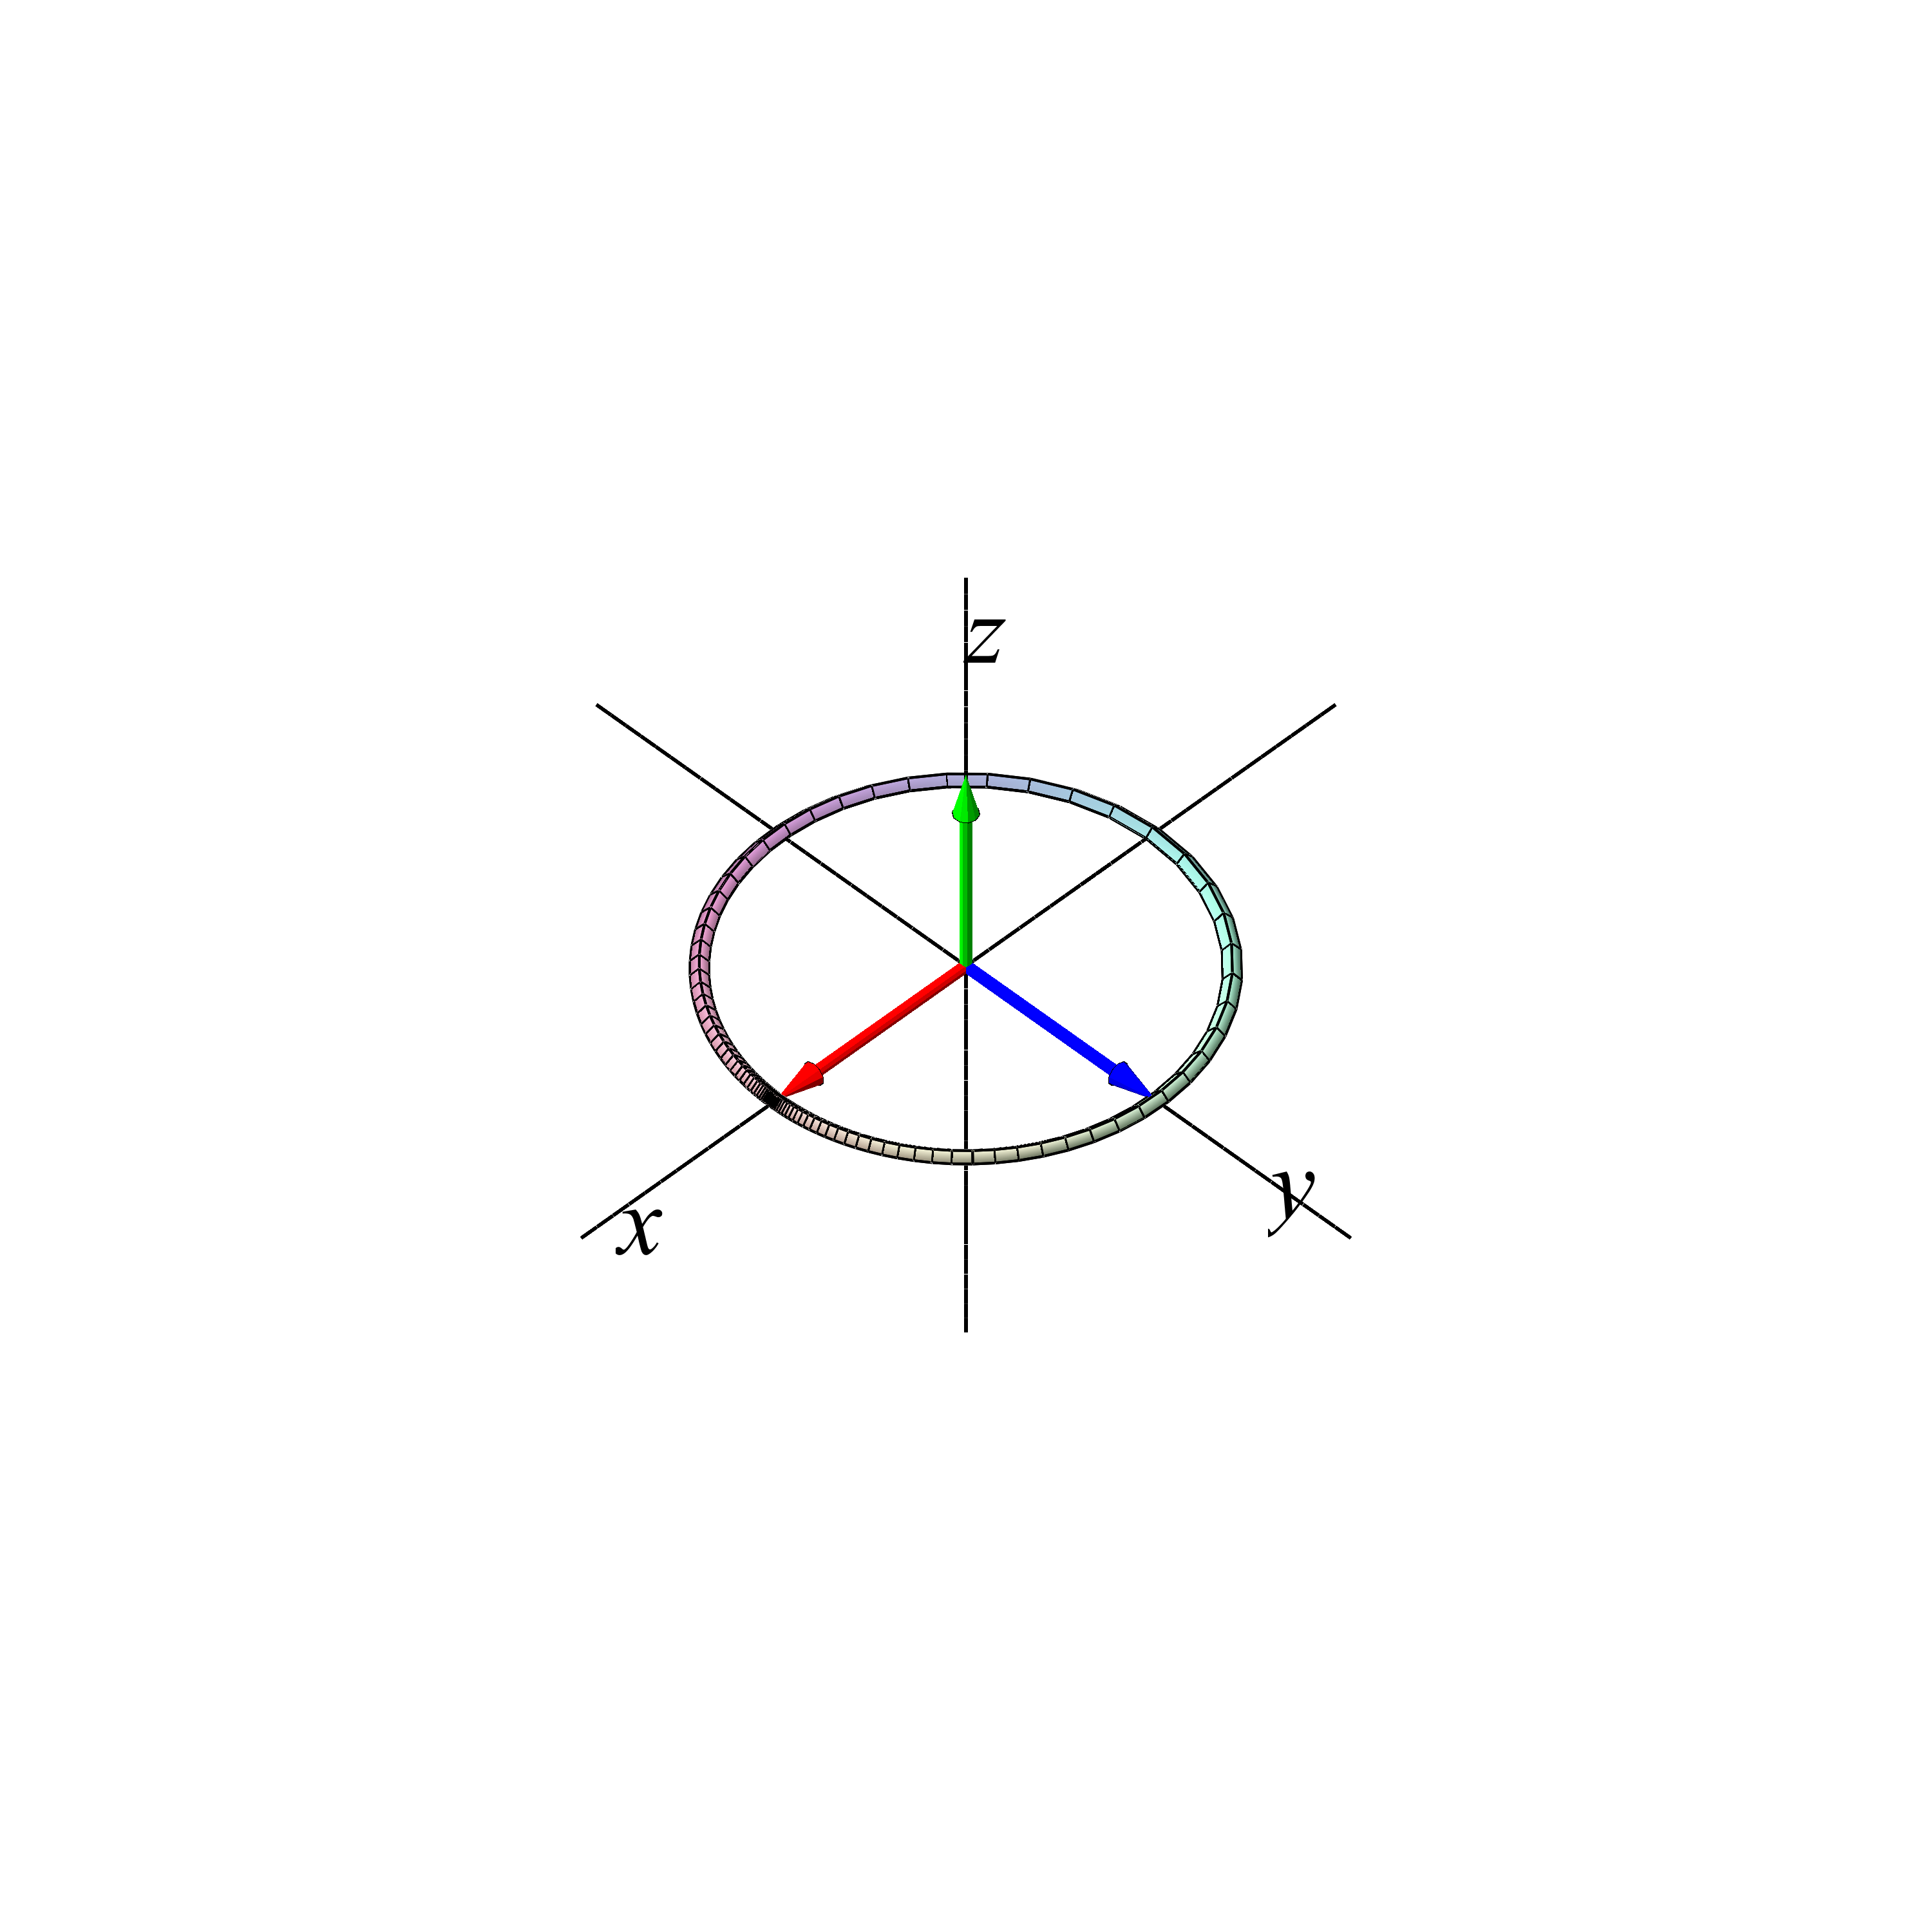
\includegraphics[height=80mm]{FIGS/plotC2}}
\begin{center}
\caption{\small{En cirkel i $(x, y)$-planen er
her parametriseret på 2 forskellige måder: ${\bf
r}_{1}(u) \, = \, \left(\cos(\pi\, u), \,
\sin(\pi \,u),\, 0\right), \, \, u \, \in [-1,\,
1]\, $, og ${\bf r}_{2}(u) \, = \,
\left(\cos(\pi\, u^{3}), \,\sin(\pi \,u^{3}),\,
0\right), \, \, u \, \in [-1, \,1]\, $.
Mar\-ke\-ringerne stammer fra den inddeling af
{\em parameterintervallet $\, [-1, 1]\,$} som
består af $100$ lige store delintervaller. Længden
af cirklen er $2\pi$ - uafhængig af
parametriseringen.}} \label{figc12}
\end{center}
\end{figure}




\begin{example}[Skruelinje] \label{exSkruelinje}
{Skruelinjen} i figur \ref{figv12} er præsenteret med 2
\emph{forskellige parametriseringer}: \begin{center} ${\bf r}_{1}(u) \, =
\, \left(\cos(2\pi u), \,\sin(2\pi u),\, \frac{\pi}{5}u\right), \,
\, u \, \in [-1,\, 1]\, \, $, og \end{center}
\begin{center} ${\bf r}_{2}(u) \, = \, \left(\cos(2\pi\, u^{3}),
\,\sin(2\pi\, u^{3}),\, \frac{\pi}{5}u^{3} \right), \, \, u \, \in
[-1,\, 1]\, $.
\end{center} Markeringerne stammer fra den inddeling af {\em
parameterintervallet $\, [-1, 1]\,$} som består af $200$ lige store
delintervaller. Kurverne er igen klart lige lange (se opgave
\ref{exercLaengde}).
\end{example}




\begin{example}[Knude] \label{exKnude}
{{Knuden}} i Figur \ref{figKnude} har den noget
komplicerede parameterfremstilling
\newline ${\bf r}(u) \, = \, \left(\, -\frac{1}{3}\cos(u) -
\frac{1}{15}\cos(5u) + \frac{1}{2}\sin(2u)\, , \, \,
\frac{1}{3}\sin(u) - \frac{1}{15}\sin(5u)-\frac{1}{2}\cos(2u)\,  ,
\, \, \frac{1}{3}\cos(3u) \, \right)\, \,  ,$ \newline hvor $\, u \,
\in \, [-\pi, \pi]$.
\end{example}

\begin{figure}[t]
\centerline{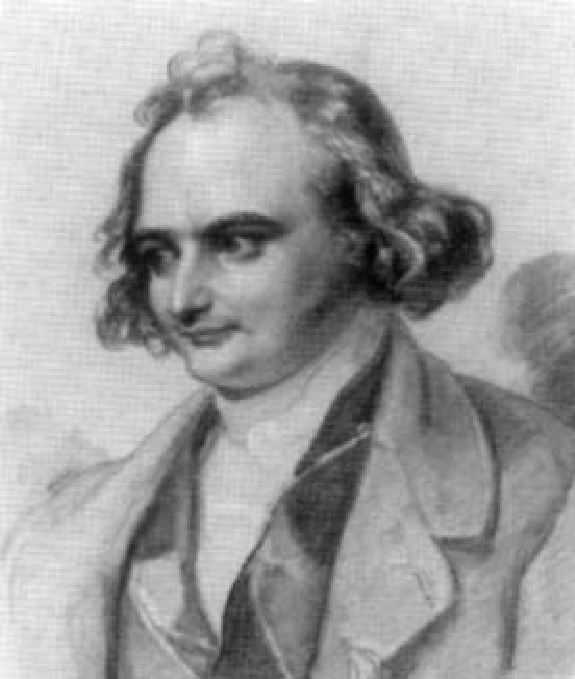
\includegraphics[height=40mm]{FIGS/PERSJacobi_3}}
\begin{center}
\caption{\small{Carl Gustav Jakob Jacobi. Se  \href{http://www-groups.dcs.st-and.ac.uk/~history/Mathematicians/Jacobi.html}{Biografi}.}} \label{figJacobi}
\end{center}
\end{figure}



\begin{figure}[ht]
\centerline{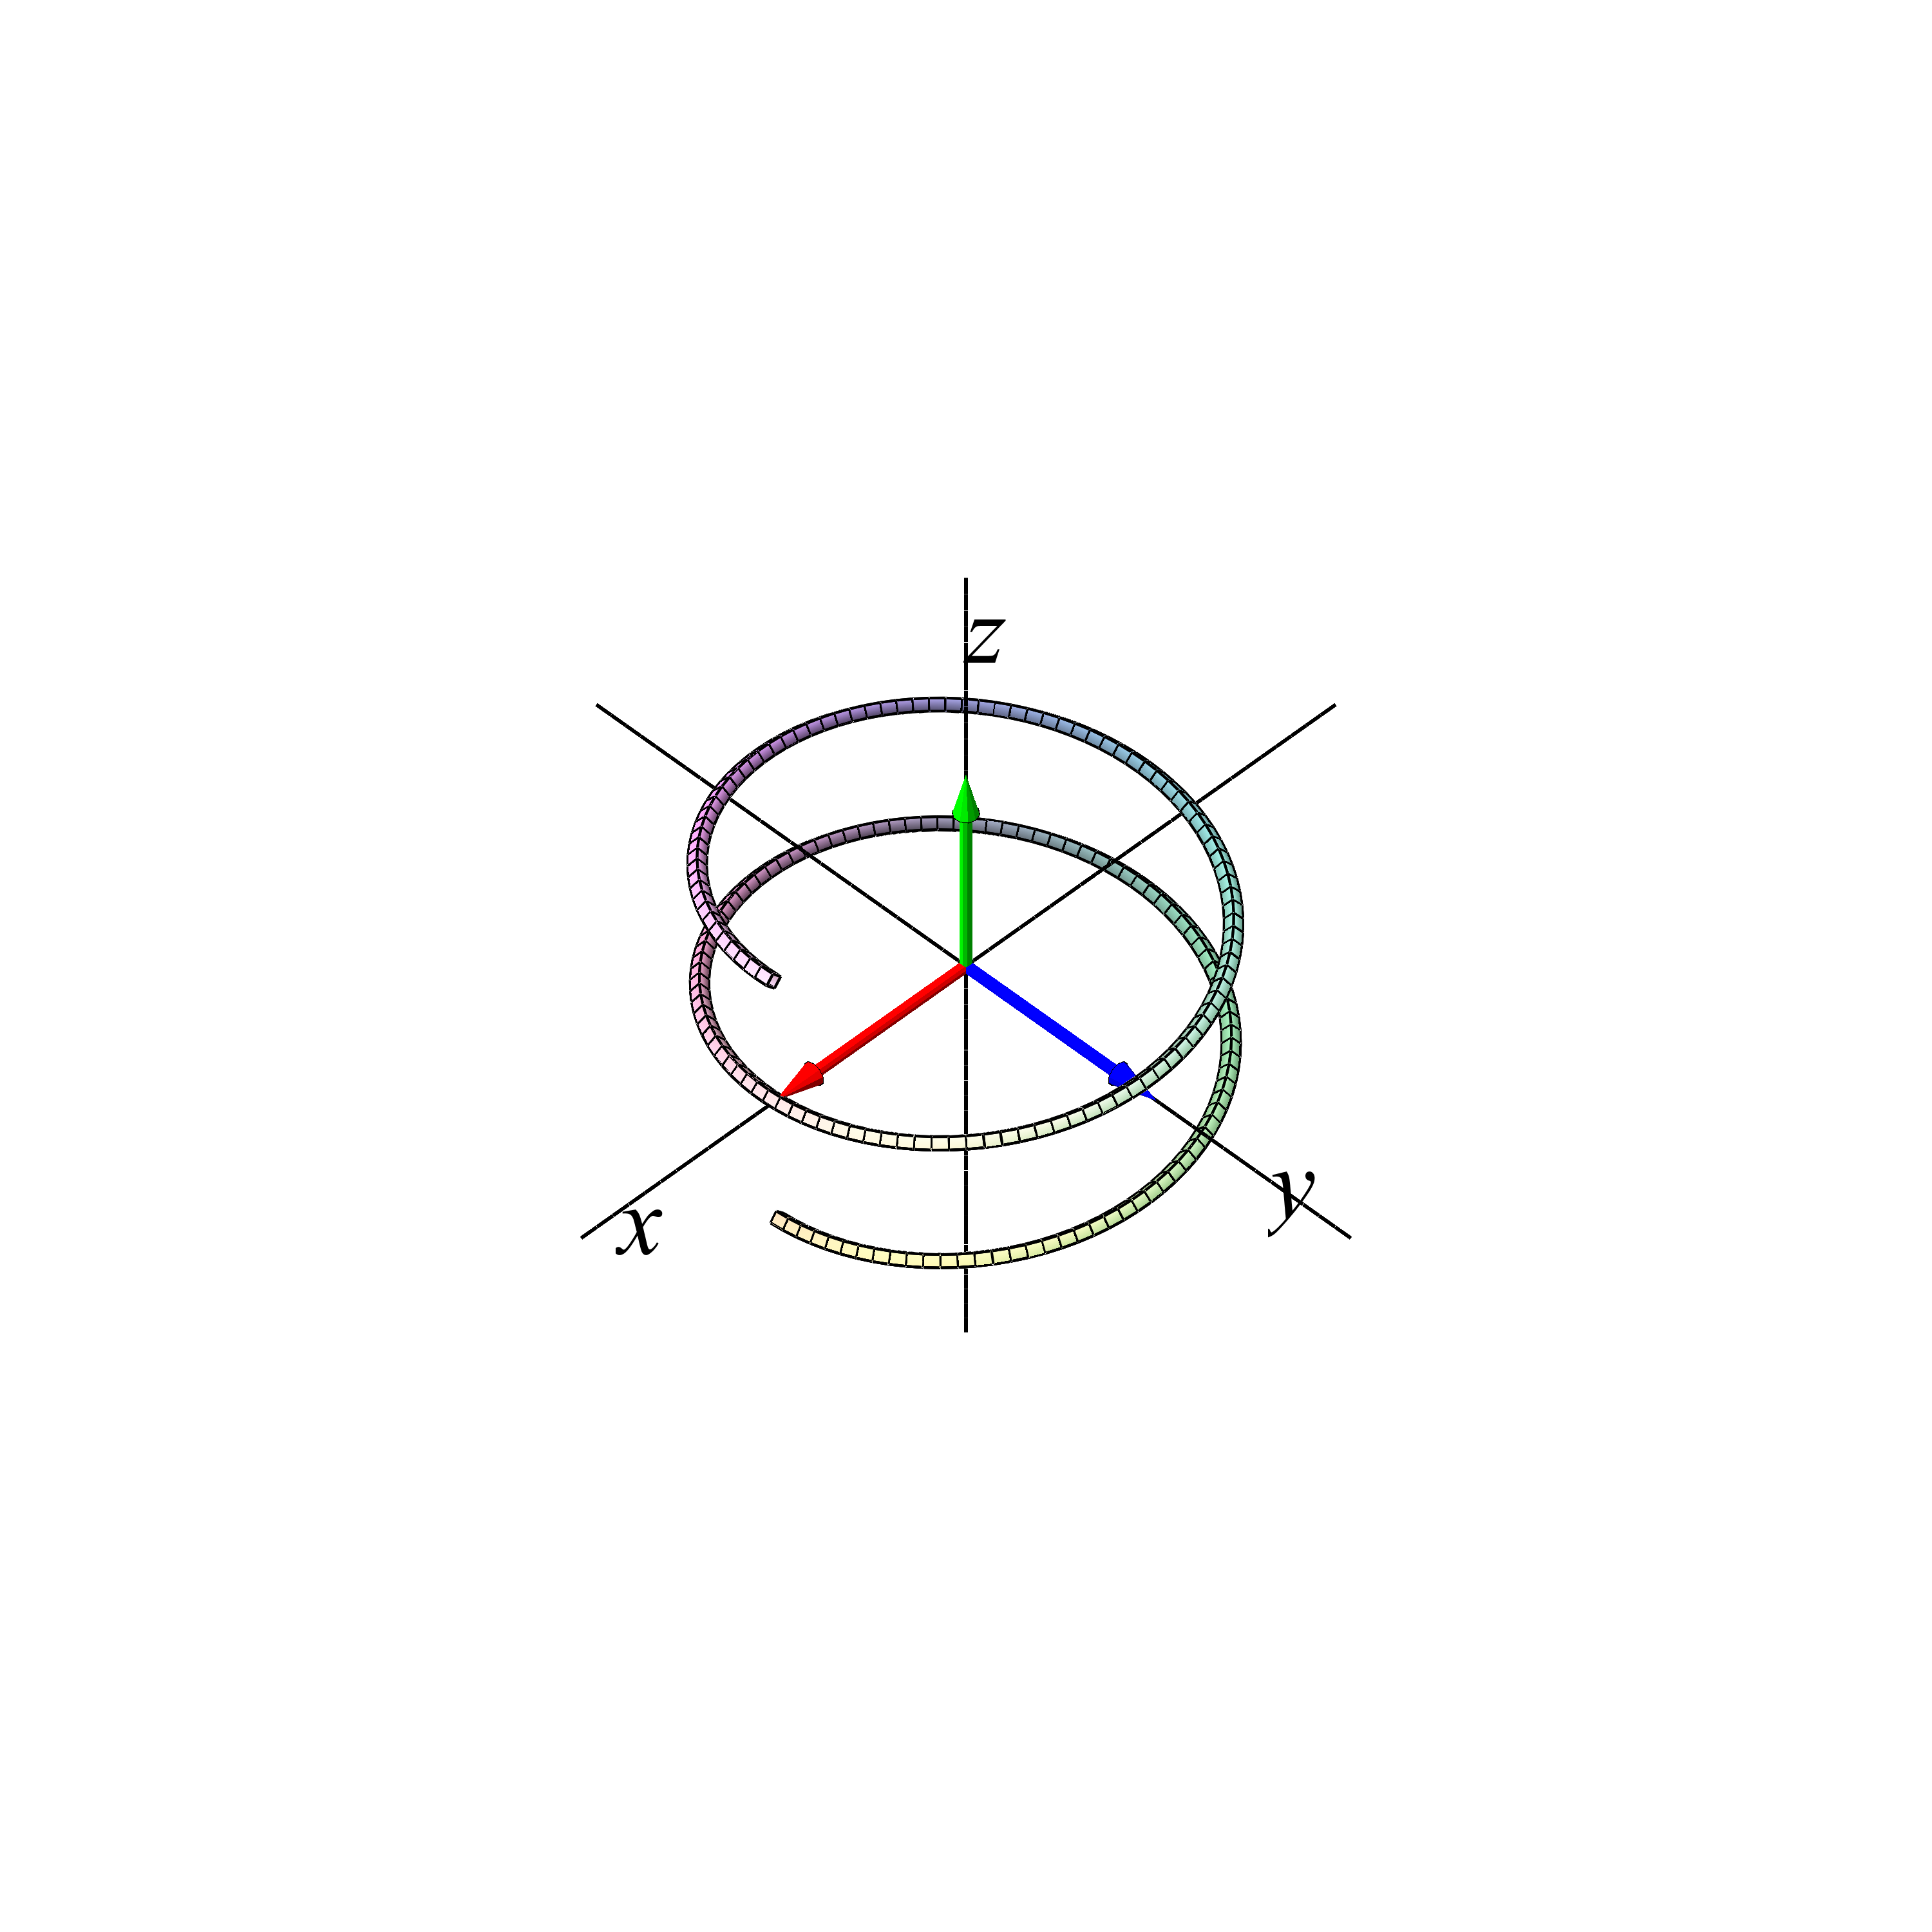
\includegraphics[height=80mm]{FIGS/plotHelix1}\, \, \, 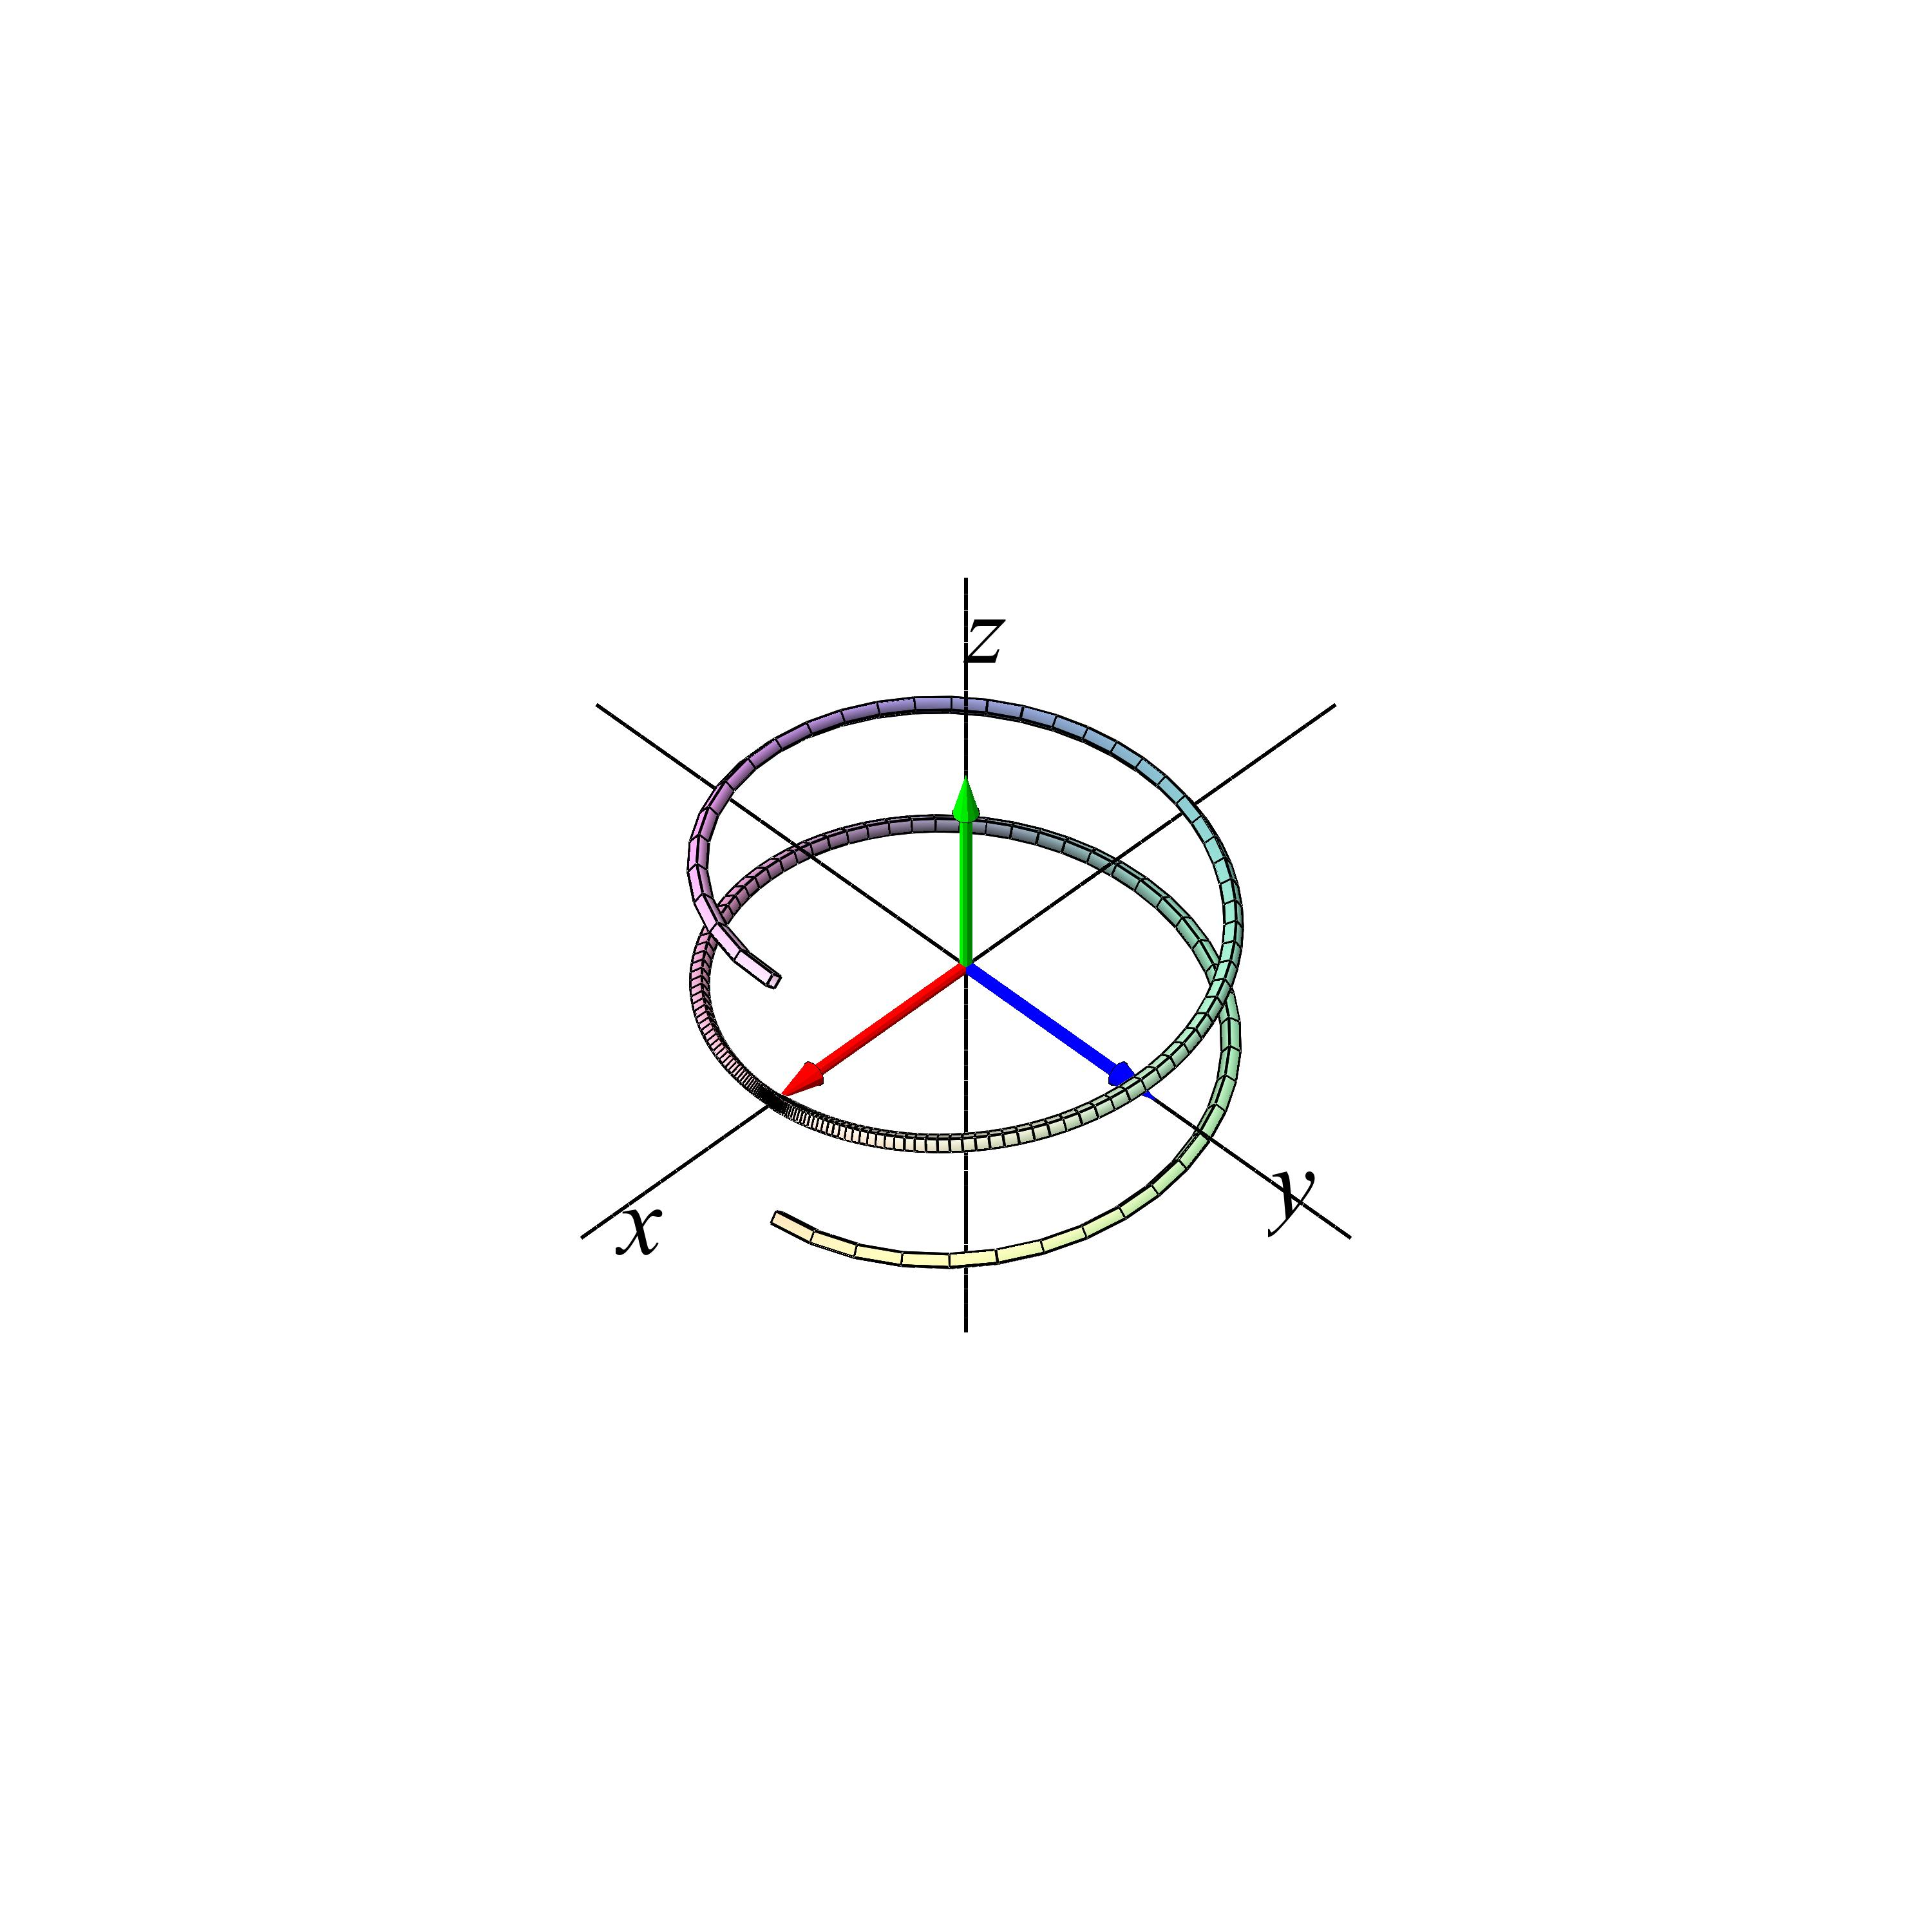
\includegraphics[height=80mm]{FIGS/plotHelix2}}
\begin{center}
\caption{\small{En skruelinje i rummet med to forskellige parametriseringer. Se
eksempel \ref{exSkruelinje}. }} \label{figv12}
\end{center}
\end{figure}


\begin{figure}[ht]
\centerline{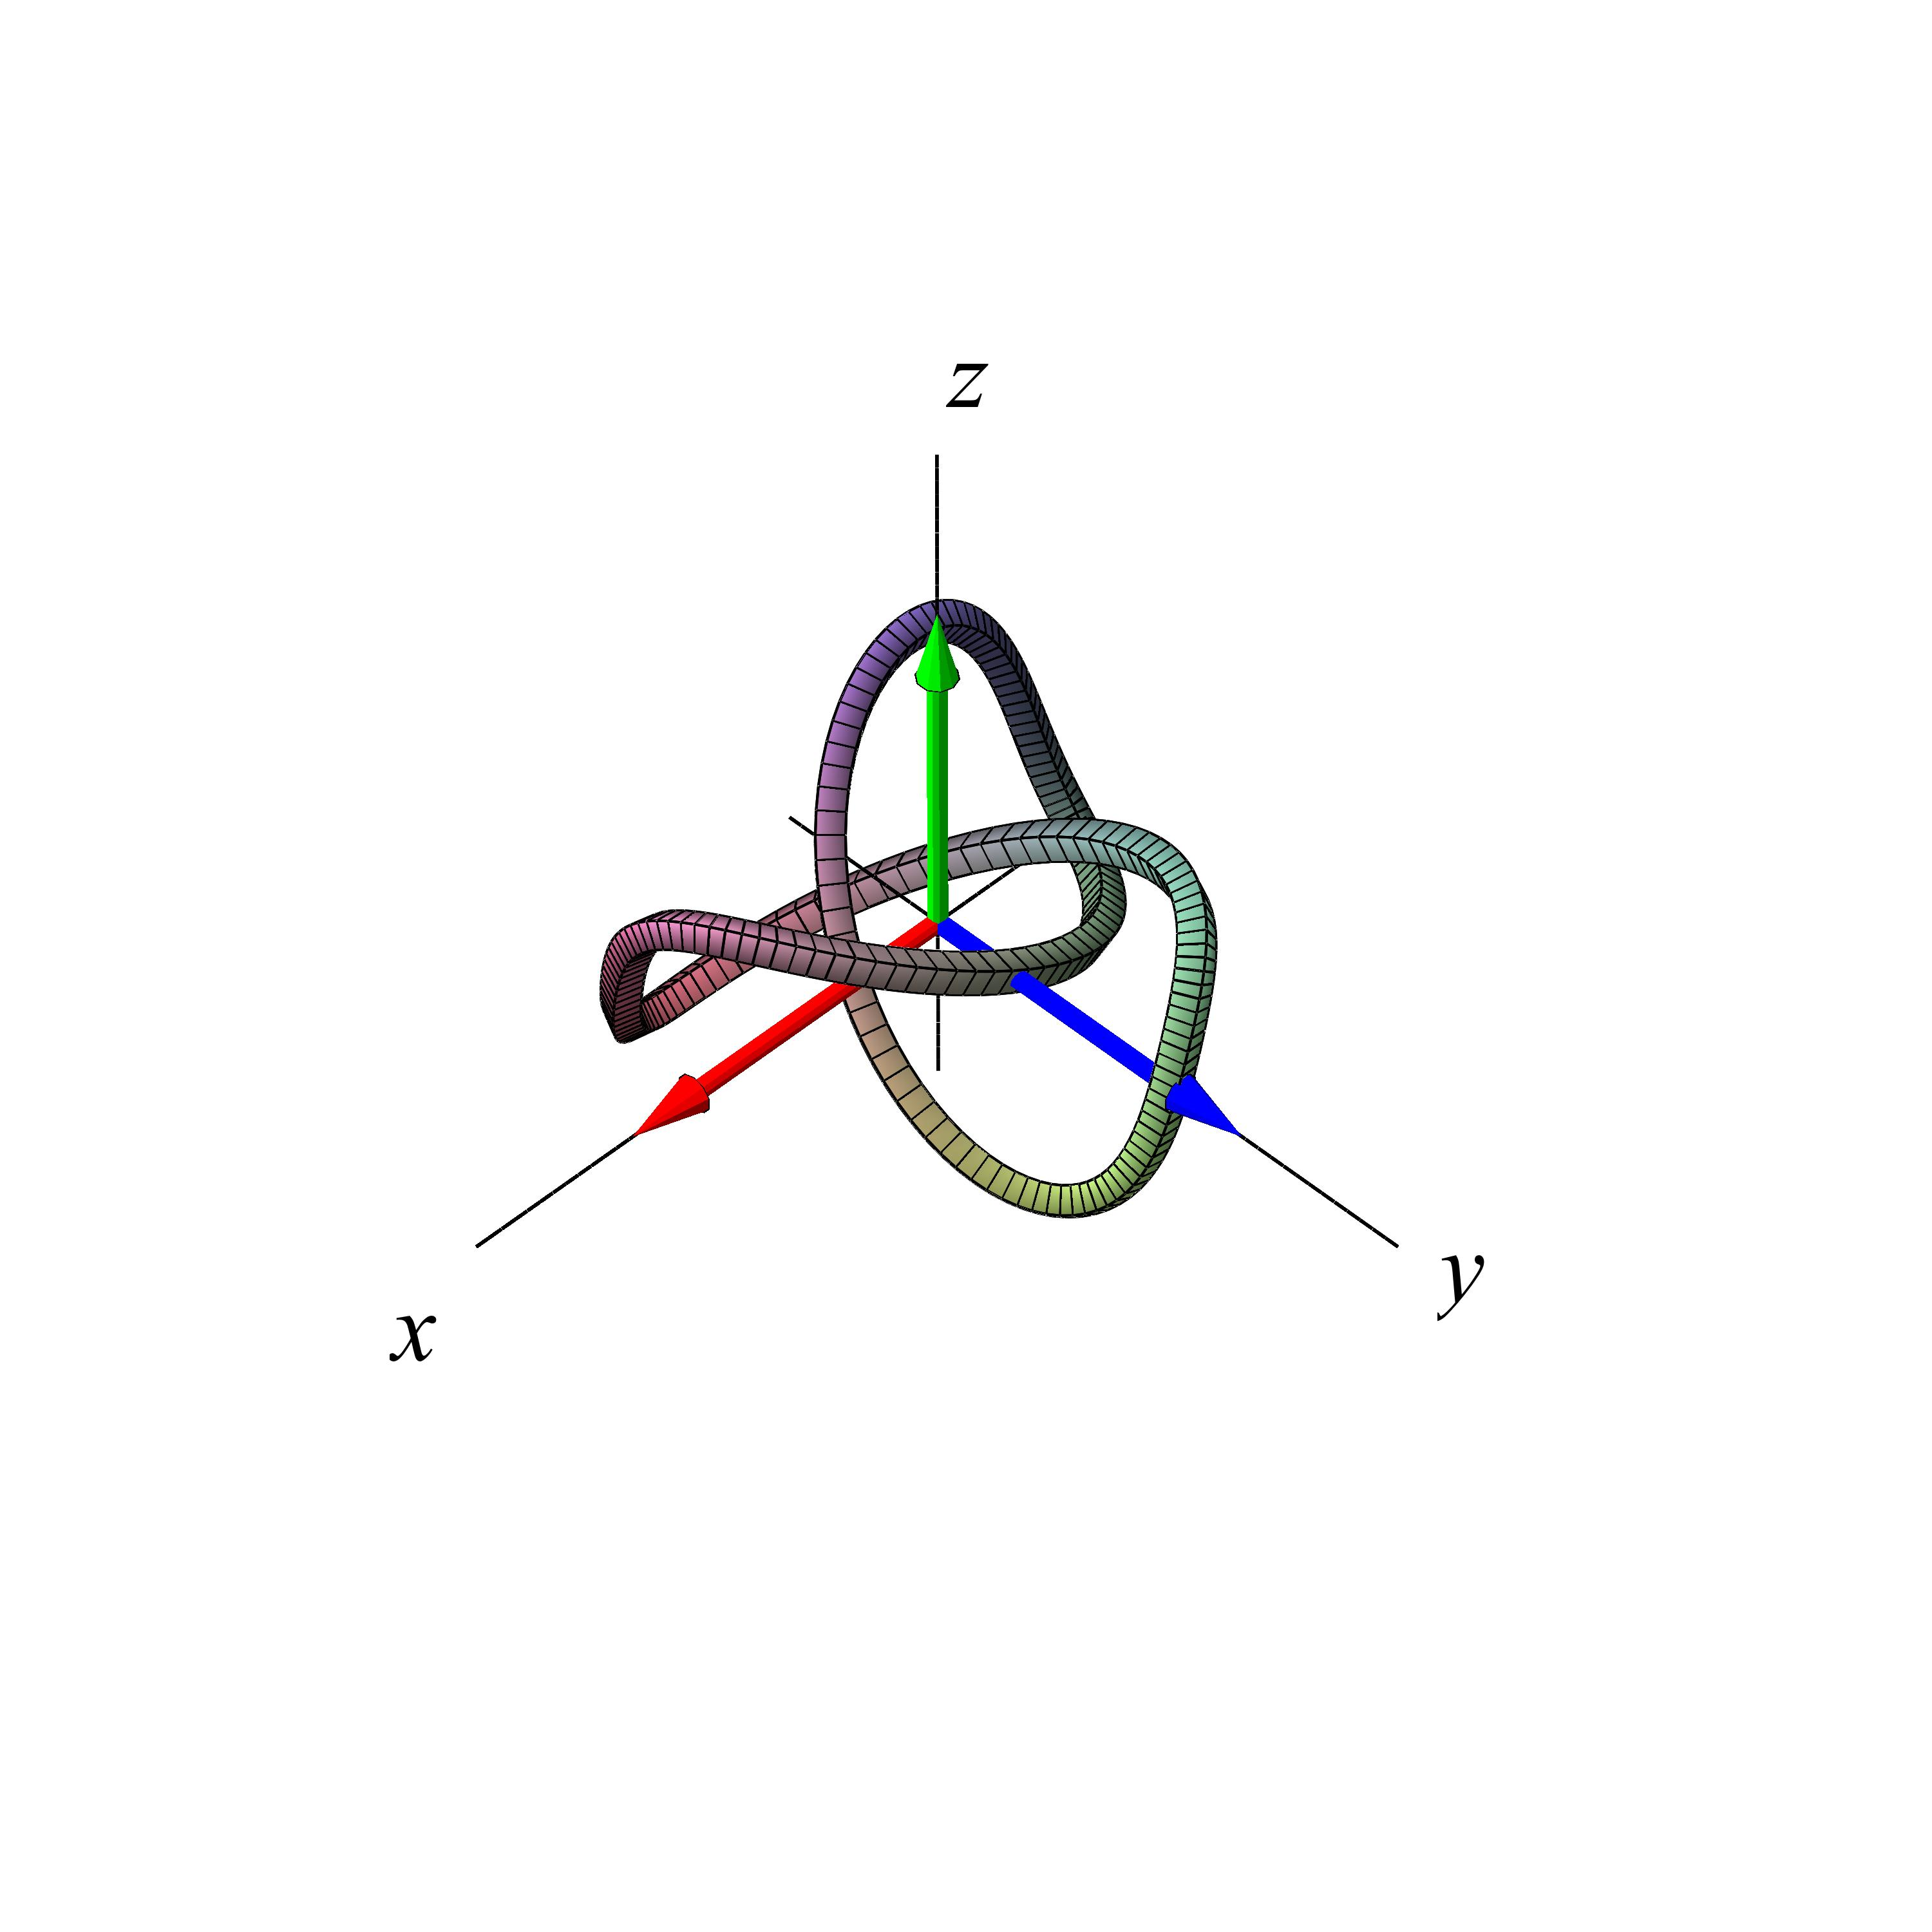
\includegraphics[height=90mm]{FIGS/plotKnude}}
\begin{center}
\caption{\small{En {knude}. Se eksempel
\ref{exKnude} }} \label{figKnude}
\end{center}
\end{figure}


Vi definerer kurveintegration på følgende måde, og motiverer definitionen i afsnit \ref{subsecMotivKurve} nedenfor:


\begin{definition}[Kurveintegral] \label{defKurveInt}
Lad $f(x,y,z)$ betegne en kontinuert funktion på $\mathbb{R}^{3}$.
{Kurveintegralet} af funk\-tio\-nen $f$ over en {parametriseret kurve}
$K_{\bf r}$ defineres ved
\begin{equation} \label{eqKurveintegral1d}
\int_{K_{\bf r}} f \, d\mu \, = \, \int_{a}^{b} f({\bf
r}(u))\,\Jac_{\bf r}(u)\,du \quad ,
\end{equation}
hvor {Jacobi-funktionen $\Jac_{\bf r}(u)$} er givet ved:
\begin{equation}
\Jac_{\bf r}(u) \, = \,  | {\bf r}'(u) | \quad .
\end{equation}
Jacobi-funktionen $\Jac_{\bf r}(u)$ betegner altså længden af tangentvektoren ${\bf r}'(u)$ til kurven på stedet
${\bf r}(u)$.
\end{definition}

\begin{aha}
Læg mærke til, at det symbol, der står på venstre side af
lighedstegnet i (\ref{eqKurveintegral1d}), {\em kun} er et {\em
symbol} for kurveintegralet. Det integral vi skal regne ud står på
højre side. Og det kan lade sig gøre at integrere, fordi både $f$,
${\bf r}$ og $ | {\bf r}' | $ er
 kontinuerte, således at integranden er kontinuert.
\end{aha}

Hvis vi indsætter ${\bf r}(u) \, = \, \left(x(u), y(u), z(u)\right)$ i udtrykket for
kurveintegralet får vi:
\begin{equation}
\int_{K_{\bf r}} f \, d\mu \, = \, \int_{a}^{b} f(x(u), y(u), z(u)
)\,\sqrt{x'(u)^{2} + y'(u)^{2} + z'(u)^{2}}\,\,du \quad.
\end{equation}



\begin{remark}
Parameterfremstillingen (\ref{eqKr}) for kurven
er \emph{regulær} hvis parameterfremstillingens
Jacobi-funktion er positiv: $\Jac_{\bf r}(u) \, = \, | {\bf r}'(u) |
> \, 0 $ for alle $u$ i det givne interval $\,[a,
b]\,$.
\end{remark}



\begin{example}[En vægtet cirkel]\label{exKurve1}
Givet funktionen $\,f(x, y, z)\, = \, 7x\,$ og et parametriseret
cirkelstykke
$$C_{\bf r}: \,\, {\bf r}(u) \, = \, \left(x(u), y(u), z(u)\right) \, = \,
\, \left(\cos(u), \,\sin(u),\, 0\right), \, \, \,  u \in
[-\dfrac{\pi}{2}, \pi] \quad.$$ Kurveintegralet af $f$ over
$C_{\bf r}$ er
\begin{equation*}
\begin{aligned}
\int_{C_{\bf r}} f \, d\mu \, = \, &\int_{-\pi/2}^{\pi} f(x(u),
y(u), z(u) )\,\sqrt{x'(u)^{2} + y'(u)^{2} + z'(u)^{2}}\,\,du \\
\, = \, &\int_{-\pi/2}^{\pi} 7\cos(u)\,\sqrt{(-\sin(u))^{2} +
(\cos(u))^{2}}\,\,du \\
  \, = \, &\int_{-\pi/2}^{\pi} 7\cos(u)\,\,du
  \, =
\, 7 \quad.
\end{aligned}
\end{equation*}
\end{example}







Som nævnt, og som vi vil godtgøre nedenfor - i afsnit \ref{subsecMotivKurve} om {\em
Motivering af kurveintegralet} - kan kurveintegraler benyttes til
at finde længder af parametriserede kurver og til at finde den
totale masse af parametriserede kurver med givne massetætheder.
Hvis massetætheden er konstant $1$ fås længden (man kan finde
længden af en sådan kurve ved at veje den):

\begin{definition}[Længden af en kurve] \label{defLaengde}
{Længden} af den parametriserede kurve
\begin{equation*}
K_{\bf r}: \quad {\bf r}(u) \, = \, \left(x(u), y(u), z(u)\right)
\quad , \, \, \,  u \in [a,b]
\end{equation*}
defineres som kurveintegralet
\begin{equation}
\Le(K_{\bf r}) \, = \, \int_{K_{\bf r}} 1 \, d\mu \, = \,
\int_{a}^{b} \, | {\bf r}'(u) | \,du \quad.
\end{equation}
\end{definition}


\begin{example}[Længde af cirkelstykke]\label{exKurve2}
Det parametriserede {cirkelstykke}
\begin{equation*}
C_{\bf r}: \,\, {\bf r}(u) \, =
\, \left(\cos(u), \,\sin(u),\, 0\right), \, \, \, u \in
[-\frac{\pi}{2}, \pi] \quad \end{equation*} har længden
\begin{equation*}
\begin{aligned}
\Le(C_{\bf r}) \, = \, \int_{C_{\bf r}} 1 \, d\mu \, = \,
&\int_{-\pi/2}^{\pi} \,\sqrt{x'(u)^{2} + y'(u)^{2} + z'(u)^{2}}\,\,du \\
\, = \, &\int_{-\pi/2}^{\pi}\,\sqrt{(-\sin(u))^{2} +
\cos(u))^{2}}\,\,du \\
  \, = \, &\int_{-\pi/2}^{\pi} 1\,\,du
  \, =
\, \frac{3\,\pi}{2} \quad.
\end{aligned}
\end{equation*}
\end{example}

\begin{example}[Multiple cirkelvindinger]\label{exKurveLang}
Den parametriserede plane kurve $$\widetilde{C}_{\bf
r}: \,\, {\bf r}(u) \, = \, \left(\cos(u),
\,\sin(u),\, 0\right), \, \, \, u \in
[-\frac{\pi}{2}, 7\pi] \quad $$ har længden
$\Le(\widetilde{C}_{\bf r}) \, = \,
\frac{15\,\pi}{2} \, $ svarende til at
parametriseringen 'lægger' det lange interval
flere gange rundt på enhedscirklen!
\end{example}


\begin{example}[Længden af en plan spiral] \label{exSpiral}
Den parametriserede plane spiral (se figur \ref{figSpiral})
$$
K_{\bf r}: \,\, {\bf
r}(u) \, = \, \left(\, u\cos(u), \,u\sin(u), \, 0 \, \right) \, , \, \, u \in
[0, \pi/2]
$$
har længden
\begin{equation}
\begin{aligned}
\Le(K_{\bf r}) \, = \, \int_{K_{\bf r}} 1 \, d\mu \, = \,
&\int_{0}^{\pi/2} \,\sqrt{x'(u)^{2} + y'(u)^{2} + z'(u)^{2}}\,\,du \\
\, = \, &\int_{0}^{\pi/2}\,\sqrt{(\cos(u) - u\sin(u))^{2} + (\sin(u) + u\cos(u))^{2}}\,\,\,du \\
\, = \, &\int_{0}^{\pi/2}\,\sqrt{1+u^{2}}\,\,\,du \\
  \, = \, & \left[(1/2)u\sqrt{1+u^2}+(1/2)\operatorname{arcsinh}(u)\right]_{0}^{\pi/2} \\
   \, = \, &  (\pi/4)\sqrt{1+(\pi/2)^2}+(1/2)\operatorname{arcsinh}(\pi/2) \\
    \, = \, &  (\pi/8)\sqrt{4+\pi^{2}}+(1/2)\ln(2)-(1/2)\ln(-\pi+\sqrt{4+\pi^{2}}) \\
    \, = \, &   2.079  \quad .
\end{aligned}
\end{equation}
\end{example}



\begin{figure}[ht]
\centerline{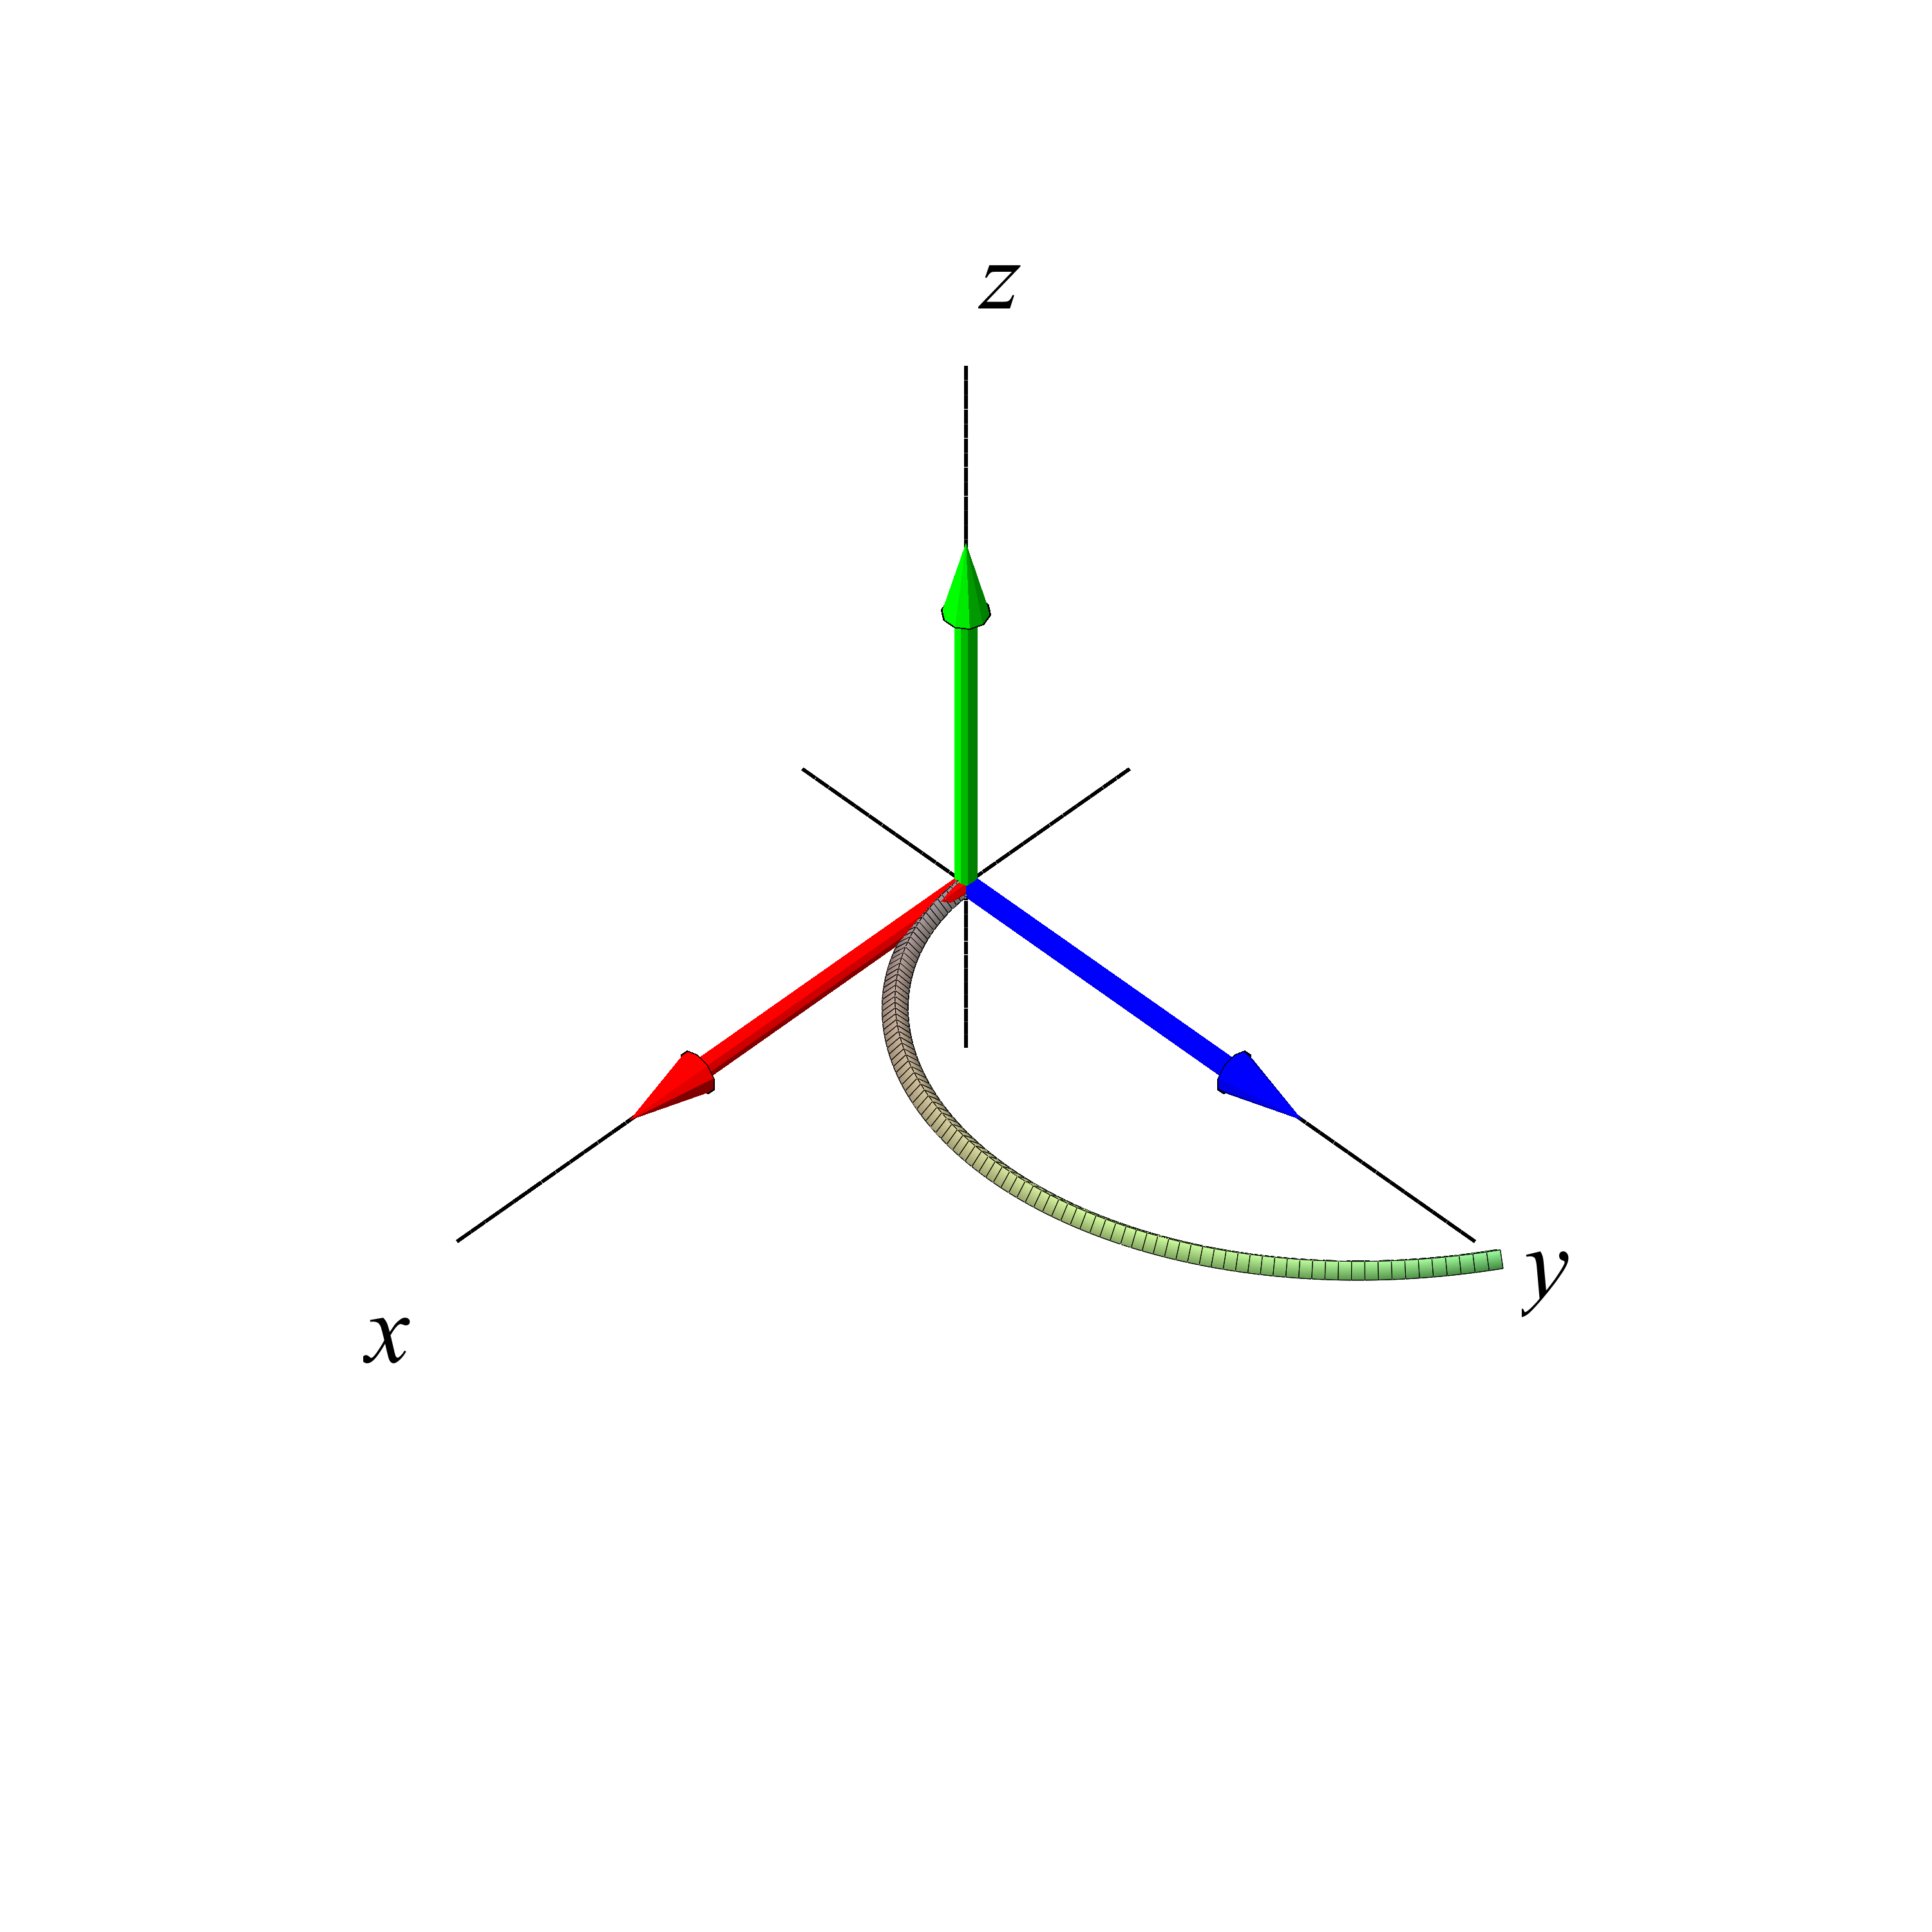
\includegraphics[height=70mm]{FIGS/plotSpiral}}
\begin{center}
\caption{\small{Del af en plan spiral. Se
eksempel \ref{exSpiral}. }} \label{figSpiral}
\end{center}
\end{figure}



\begin{example}[Ellipsens længde] \label{exEllipse}
{Længden af en ellipse}. Den parametriserede ellipse (se Figur \ref{figEllipse})
$$
K_{\bf r}: \,\, {\bf
r}(u) \, = \, \left(\, a\cos(u), \,b\sin(u), \, 0 \, \right) \, , \, \, u \in
[-\pi, \pi]
$$
har længden
$$
\begin{aligned}
\Le(K_{\bf r}) \, = \, \int_{K_{\bf r}} 1 \, d\mu \, = \,
&\int_{-\pi}^{\pi} \,\sqrt{x'(u)^{2} + y'(u)^{2} + z'(u)^{2}}\,\,du \\
\, = \, &\int_{-\pi}^{\pi}\,\sqrt{a^2\sin^2(u) +
b^2\cos^2(u)}\,\,\,du \\
  \, = \, & 4aE\left(\sqrt{1- \left(\frac{b}{a}\right)^2}\right)\quad,
\end{aligned}
$$
hvor $E$ betegner det såkaldte fuldstændige elliptiske integral af 2. orden.
Om funktionen $E(u)$ nævner vi her kun, at funktionsværdien i $u=0$ er $E(0) \, = \, \pi/2$, således at ovenstående resultat betyder, at når ellipsen specielt er en cirkel, dvs. når $a \, = \, b$, så får vi den korrekte
omkreds af cirklen med radius $a$: $L\, = \, 2\pi a \,$.
\end{example}



\begin{figure}[ht]
\centerline{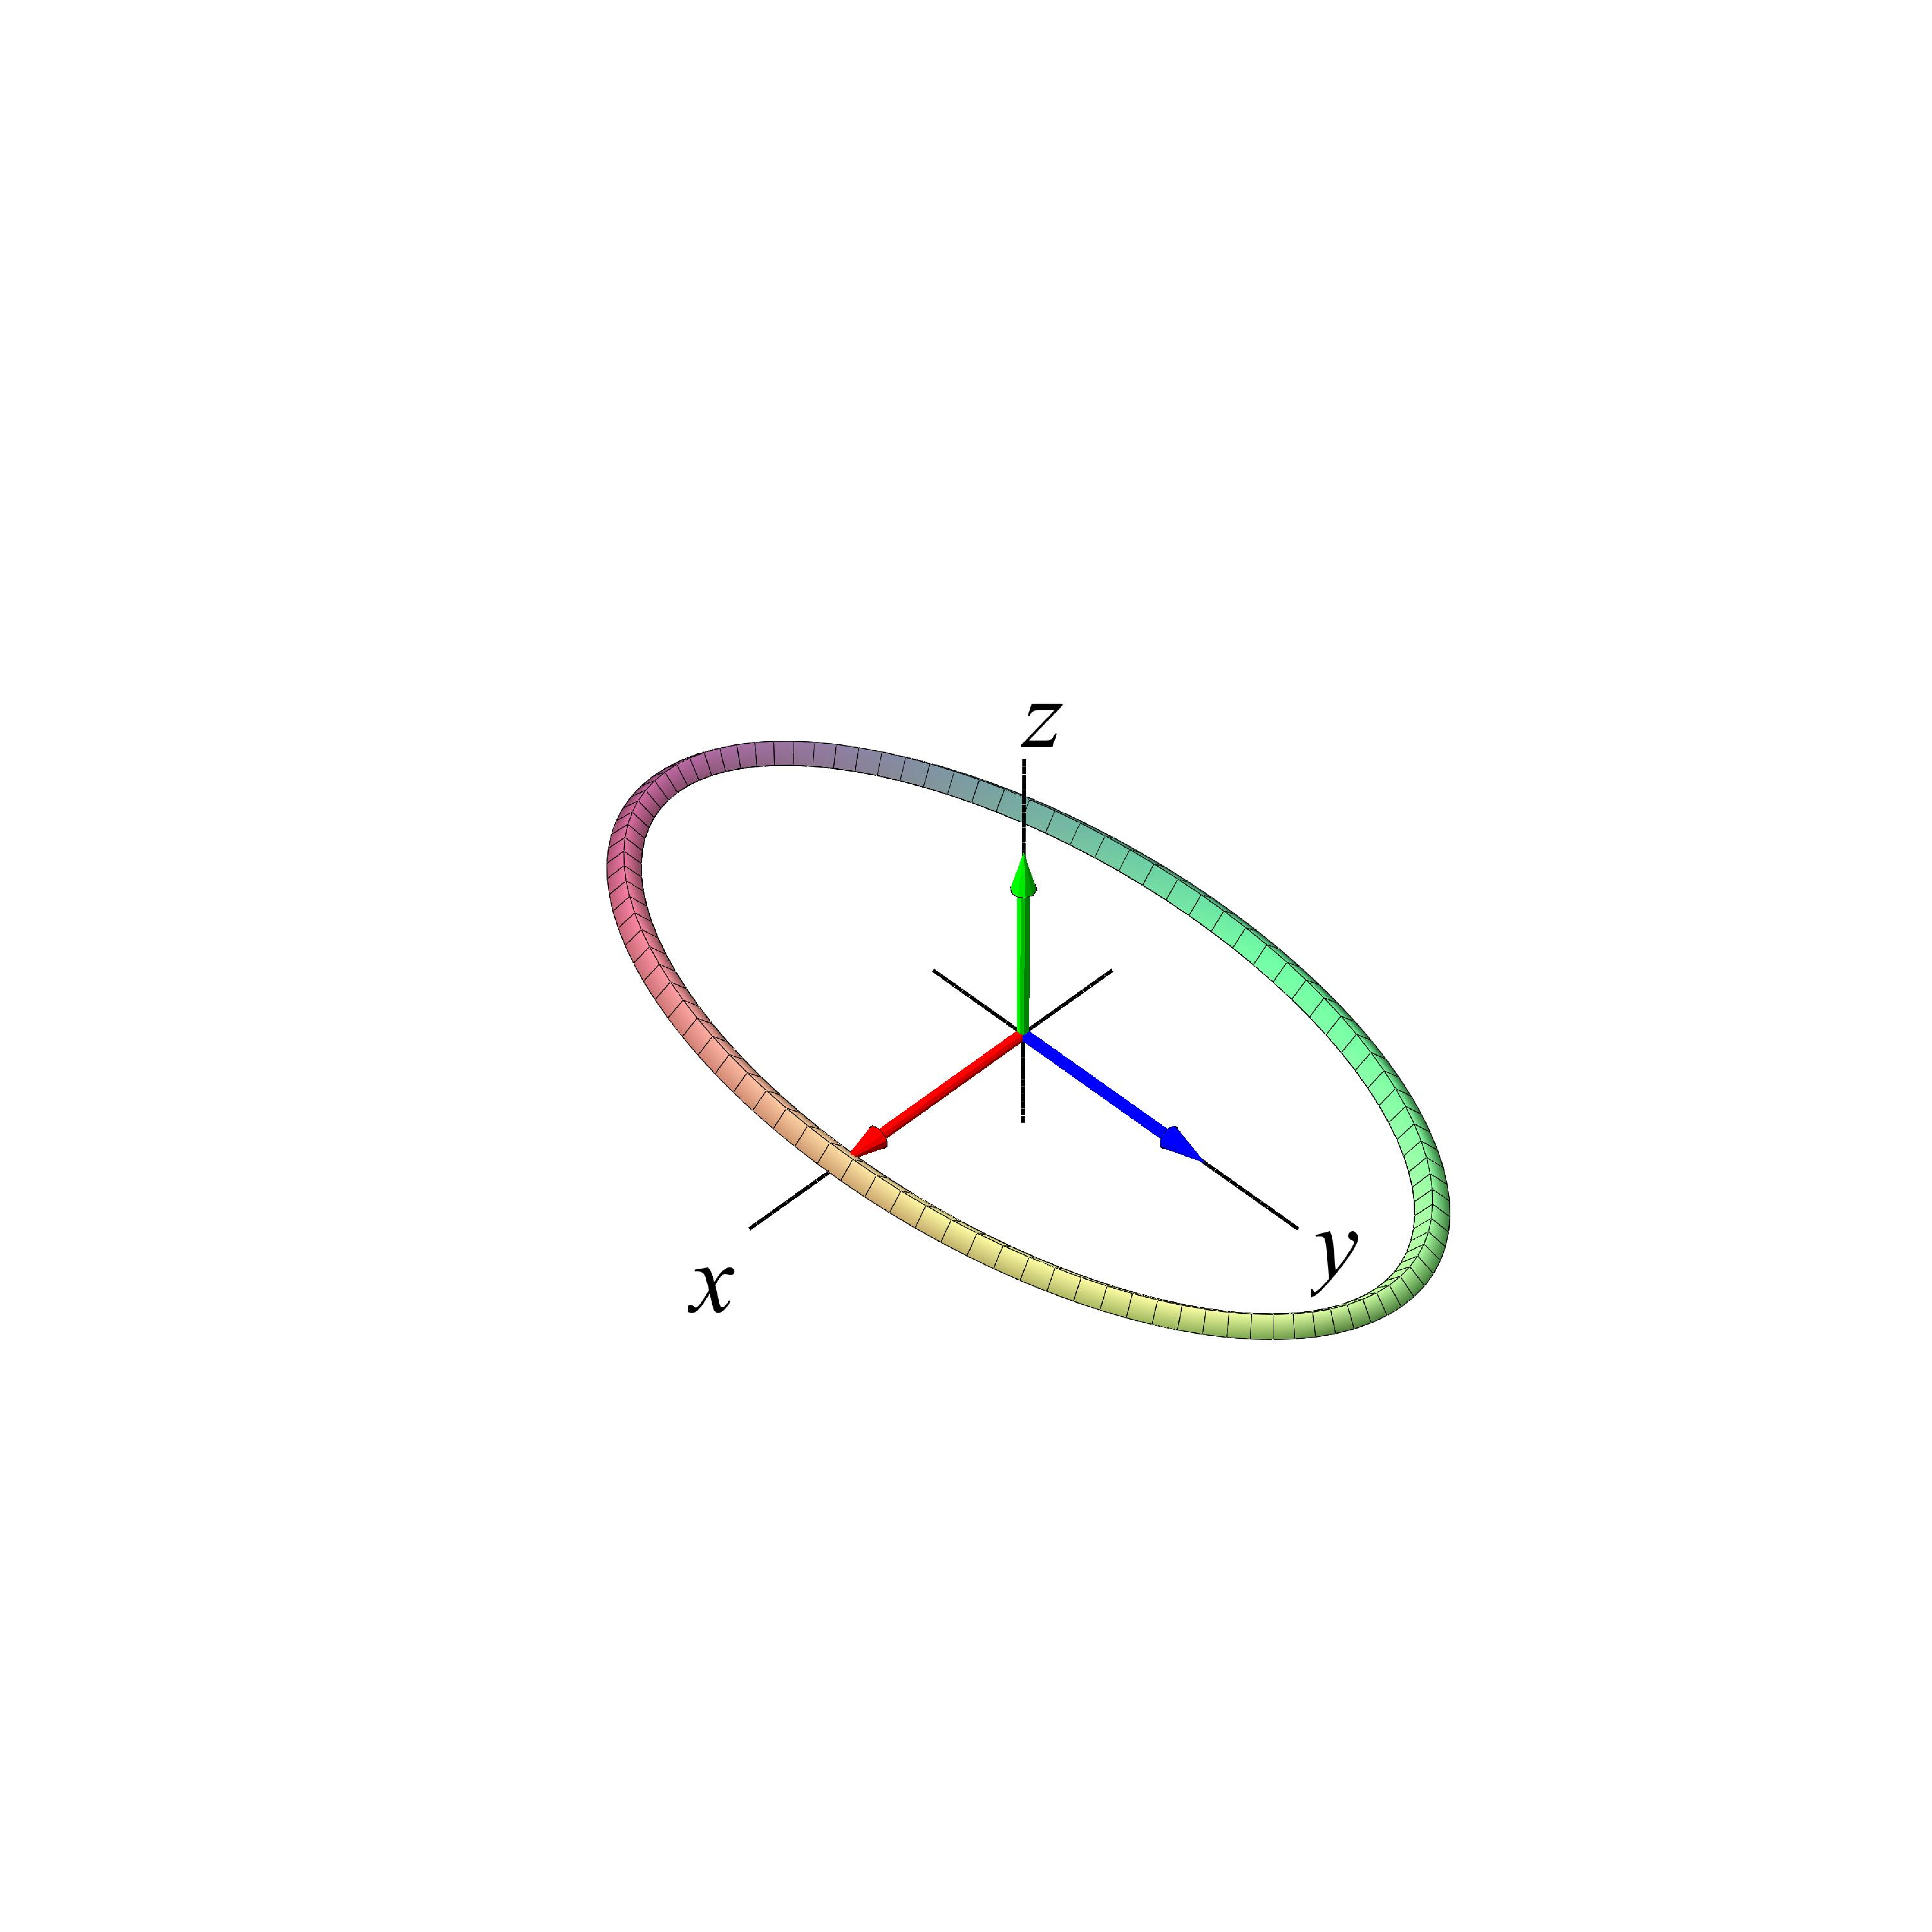
\includegraphics[height=70mm]{FIGS/plotEllipse}\, \, \, 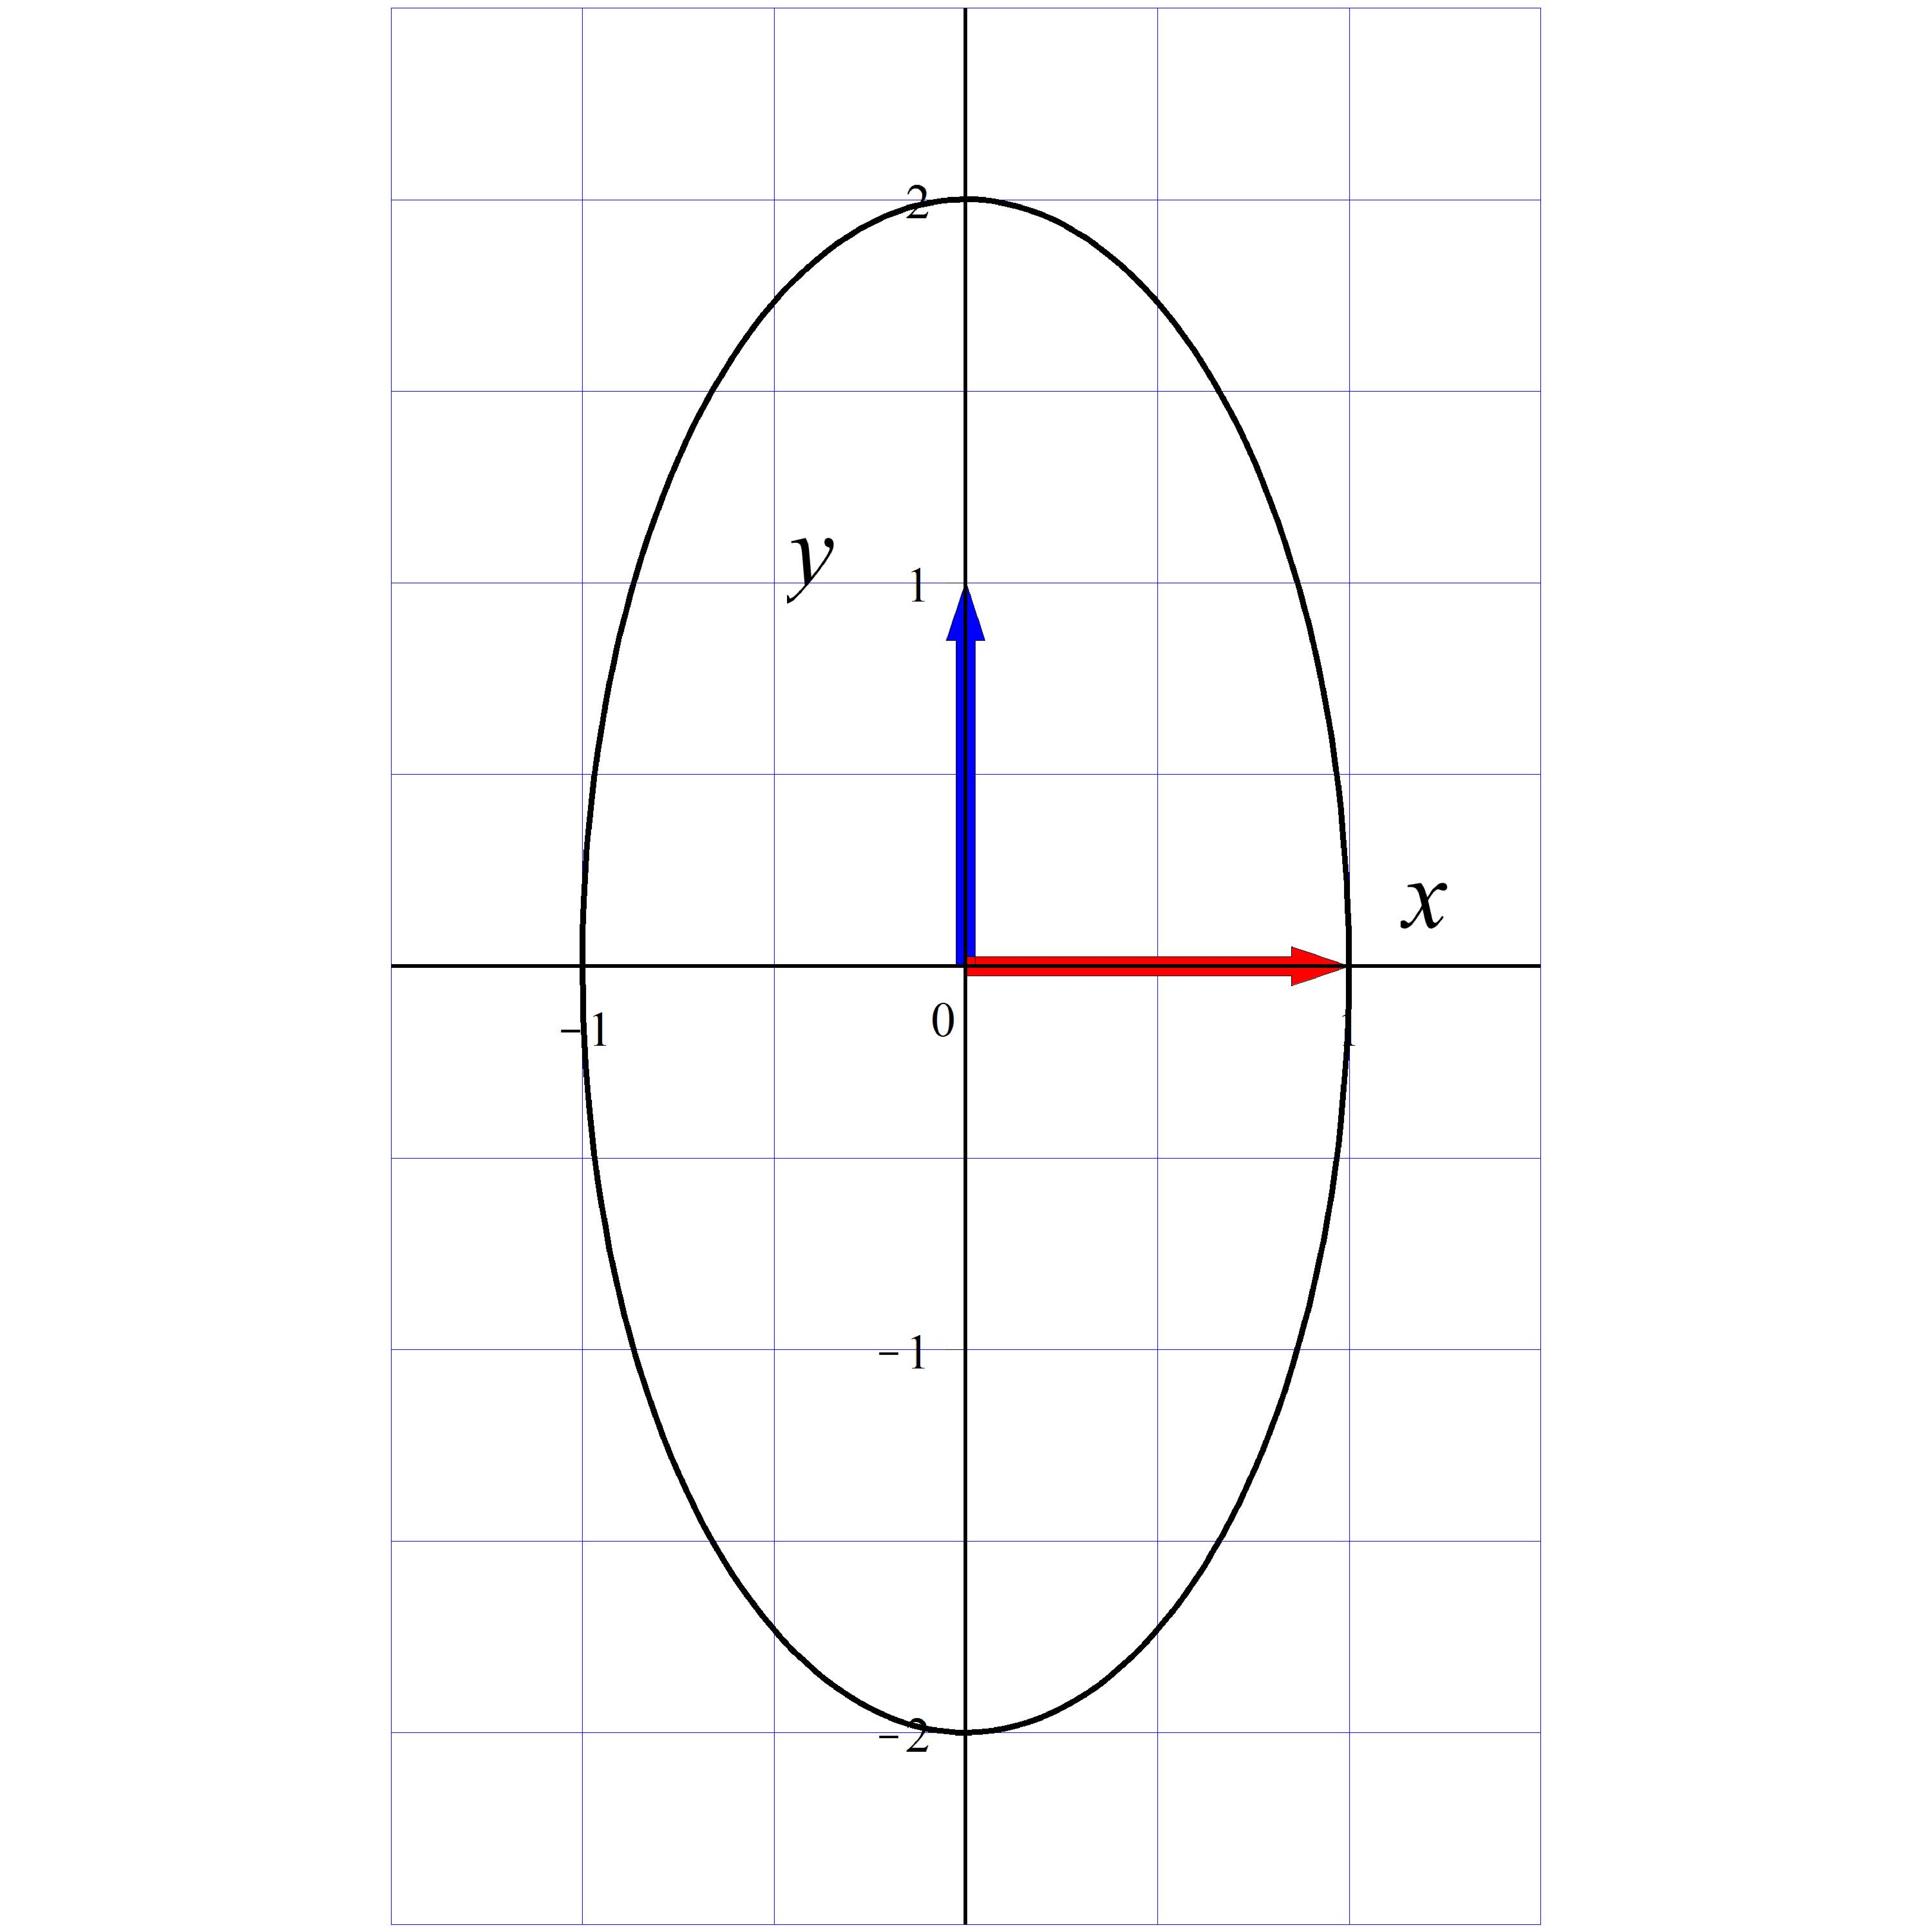
\includegraphics[height=75mm]{FIGS/plotEllip2d}}
\begin{center}
\caption{\small{En ellipse med halvakser $a=1$ og $b=2$. Se
eksempel \ref{exEllipse}. }} \label{figEllipse}
\end{center}
\end{figure}






\begin{example}[Skruelinjens længde]\label{exKurve3}
Den parametriserede skruelinje
$$K_{\bf r}: \,\, {\bf
r}(u) \, = \, \left(\cos(u), \,\sin(u),\, u\right), \, \, \, u \in
[-2\pi, 2\pi]
$$ har længden
$$
\begin{aligned}
\Le(K_{\bf r}) \, = \, \int_{K_{\bf r}} 1 \, d\mu \, = \,
&\int_{-2\pi}^{2\pi} \,\sqrt{x'(u)^{2} + y'(u)^{2} + z'(u)^{2}}\,\,du \\
\, = \, &\int_{-2\pi}^{2\pi}\,\sqrt{(-\sin(u))^{2} +
(\cos(u))^{2} + 1}\,\,\,du \\
  \, = \, &\int_{-2\pi}^{2\pi} \sqrt{2}\,\,du
  \, =
\, 4\pi\,\sqrt{2} \quad.
\end{aligned}
$$
\end{example}



\begin{definition}[En-entydig parameterfremstilling] \label{defEnEntydigKurve}
Parameterfremstillingen i (\ref{eqKr}) for kurven $K_{\bf r}$ siges
at være {\em{{en-entydig}}} hvis der for alle $u_{1} \in [a, b]$ og
for alle $u_{2} \in [a, b]$ gælder følgende:
\begin{equation}
u_{1} \, \neq \, u_{2} \quad \text{medfører at} \quad {\bf r}(u_{1}) \, \neq \, {\bf r}(u_{2}) \quad .
\end{equation}
\end{definition}

\begin{exercise}
Hvilke af parameterfremstillingerne i figurerne \ref{FigIntLine123},
\ref{figc12}, og \ref{figv12}, henholdsvis i eksemplerne
\ref{exKurve2}, \ref{exKurveLang}, og \ref{exKurve3}, er
en-entydige?
\end{exercise}


\begin{exercise}
\label{exercLaengde} Vis, at Definition \ref{defLaengde} giver samme
længde for de tre parametriseringer af linje\-styk\-ket i figur
\ref{FigIntLine123}, samme længde af de to cirkelstykker i figur
\ref{figc12} og samme længde af de to skruelinjer i figur
\ref{figv12}.
\end{exercise}

\begin{exercise}
Find længden (med 3 decimaler) af knuden i figur \ref{figKnude}.
\end{exercise}



\begin{exercise}
Find regulære, en-entydige parameterfremstillinger af linjestykket
(figur \ref{FigIntLine123}), cirklen (figur \ref{figc12}), og
skruelinjen (figur \ref{figv12}), således at alle parameterfremstillingerne har
det fælles parameterinterval $\,[0, \pi\,] $ .
\end{exercise}

%%%%%%%%%%%%%%%%%%%%%%%%%%%%%%%%%%%%%%%%%%%%%
%%%%%%%%%%%%%%%%%%%%%%%%%%%%%%%%%%%%%%%%%%%%%
%%%%%%%%%%%%%%%%%%%%%%%%%%%%%%%%%%%%%%%%%%%%%

\subsection{Motivering af kurveintegralet} \label{subsecMotivKurve}
Hvis vi deler intervallet $[a, b]$ i $n$
lige store dele, så har hvert delinterval længden $\delta_{u} \, =
\, (b-a)/n$ og delepunkternes koordinater i $[a, b]$ bliver:
\begin{equation}
\begin{aligned}
u_{1} \, &= \, a , \\ u_{2} \, &= \, u_{1} + \delta_{u} \, = \, a
+
\delta_{u}, \\
u_{3} \, &= \, u_{2} + \delta_{u} \, = \, a + 2\delta_{u}, \\
u_{4} \, &=
\, u_{3} + \delta_{u} \, = \, a + 3\delta_{u}, \\
 &.... \\
 b \, &= \,
u_{n} + \delta_{u} \, = \, a + n\delta_{u} \quad .
\end{aligned}
\end{equation}

Med hver af disse fast valgte værdier af $u_{i}$ som udviklingspunkt
kan vi nu bruge Taylor's grænseformel for hver af de $3$ koordinat-funktioner $x(u)$, $y(u)$, og $z(u)$ for ${\bf
r}(u) \, = \, \left(x(u), y(u), z(u)\right)$ til første orden og med de
tilhørende epsilon-funktioner som følger, se \tref{NUID32-tn17}{eNote}:
\begin{equation}
\begin{aligned}
x(u) \, &= \, x(u_{i}) + x'(u_{i})\,(u - u_{i}) +
\varepsilon_{x}(u-u_{i})\cdot | u-u_{i} | \\
y(u) \, &= \, y(u_{i}) + y'(u_{i})\,(u - u_{i}) +
\varepsilon_{y}(u-u_{i})\cdot | u-u_{i} | \\
z(u) \, &= \, z(u_{i}) + z'(u_{i})\,(u - u_{i}) +
\varepsilon_{z}(u-u_{i})\cdot | u-u_{i} |  \quad .
\end{aligned}
\end{equation}





Disse $3$ formler  kan vi samle og udtrykke med
vektor-notation således:
\begin{equation} \label{eqTaylor1}
{\bf r}(u) \, = \, {\bf r}(u_{i}) + \, {\bf r}'(u_{i})\cdot(u-u_{i})
+ \, {\bm{\varepsilon}}_{i}(u-u_{i})\cdot\rho_{i} \quad ,
\end{equation}
hvor  vi bruger den korte skrivemåde $\, \rho_{i} =  | u - u_{i} |
\, =\, \sqrt{(u - u_{i})^{2}}\, $ for  afstanden  mellem den
variable værdi $\,u\,$ og den faste værdi $\,u_{i}\,$ i
parameterintervallet. Desuden gælder at vektoren $\,{\bm{\varepsilon}}_{i}(u -
u_{i}) \, = \, (\,\varepsilon_{x}(u-u_{i}),\,
\varepsilon_{y}(u-u_{i}), \, \varepsilon_{z}(u-u_{i})\,)\,  \to \,
(0, 0, 0) \, = \, {\bf{0}}$ for $u \to u_{i}\,$ . \\

Hvert del-interval $[u_{i}, u_{i}+\delta_{u}]$ fra $u$-aksen  afbildes på
kurve-{\em stykket} $\, {\bf r}(u)$, $u \in[u_{i},
u_{i}+\delta_{u}]\, $, og dette kurve-stykke kan vi approksimere med
den lineære del af udtrykket i (\ref{eqTaylor1}), som fås ved at
fjerne ${\bm{\varepsilon}}_{i}$-bidraget fra højre side i
(\ref{eqTaylor1}):
\begin{equation}\label{eqApp}
{\bf r}_{\app_{\,i}}(u)\, = \, {\bf r}(u_{i}) + \, {\bf
r}'(u_{i})\cdot(u-u_{i})\,\, , \quad u \, \in \, [u_{i},
u_{i}+\delta_{u}]\quad .
\end{equation}
Se figurerne \ref{figCircApprox123} og \ref{figcircAppB123} hvor de
approksimerende linjestykker er vist for en parametriseret cirkel,
for to forskellige parametriseringer og for forskellige værdier af
$n$. Det $i$'te linjestykke har pr. definition kontakt med kurven i
sit ene endepunkt. Det kalder vi kontaktpunktet for linjestykket.

%%%%%%%%%%%%%%%%%%%%%%%%%%%%%%%%%%%%%%%
%%%%%%%%%%%%%%%%%%%%%%%%%%%%%%%%%%%%%%%

\subsubsection{Længden af en kurve}\label{subsecLengthCurve}
Hvert enkelt af de i alt $n$ approksimerende
linjestykker har en længde, se Figur
\ref{figCircApprox123}. Længden af det $i$'te
linjestykke er ifølge (\ref{eqApp})
\begin{equation}
\Delta \Le_{i} \, = \,  | {\bf r}_{\app_{\,i}}(u_{i}+\delta_{u})
- {\bf r}_{\app_{\,i}}(u_{i}) |  \, = \,  | {\bf r}'(u_{i})
| \cdot\delta_{u} \quad .
\end{equation}

Summen af disse $n$ længder er (for store værdier af $n$) klart en god approksimation til
længden af kurven, således at vi kan skrive
\begin{equation}
\Le_{\app}(n)\, = \,   \sum_{i=1}^{n} \Delta \Le_{i} \, = \,
\sum_{i=1}^{n} | {\bf r}'(u_{i}) | \cdot\delta_{u} \quad,
\end{equation}
Da ovenstående sum er en  integralsum (se \tref{NUID36-tn21}{eNote})
for den kontinuerte funktion $\, | {\bf r}'(u) | \, $ over
intervallet $\, [a, b]\, $, opnås i grænsen, hvor $n$ går imod
uendelig:
\begin{equation}
\Le_{\app}(n)\,  \to \, \Le\, = \, \int_{a}^{b} | {\bf r}'(u) | \,du
\quad \text{for} \quad n \to \infty \quad.
\end{equation}

Vi har dermed motiveret definitionen af længden af en kurve som
angivet ovenfor, nemlig som kurveintegralet af den konstante
funktion $1$ over den parametriserede kurve.

%%%%%%%%%%%%%%%%%%%%%%%%%%%%%%%%%
%%%%%%%%%%%%%%%%%%%%%%%%%%%%%%%%%%5

\begin{figure}[ht]
\centerline{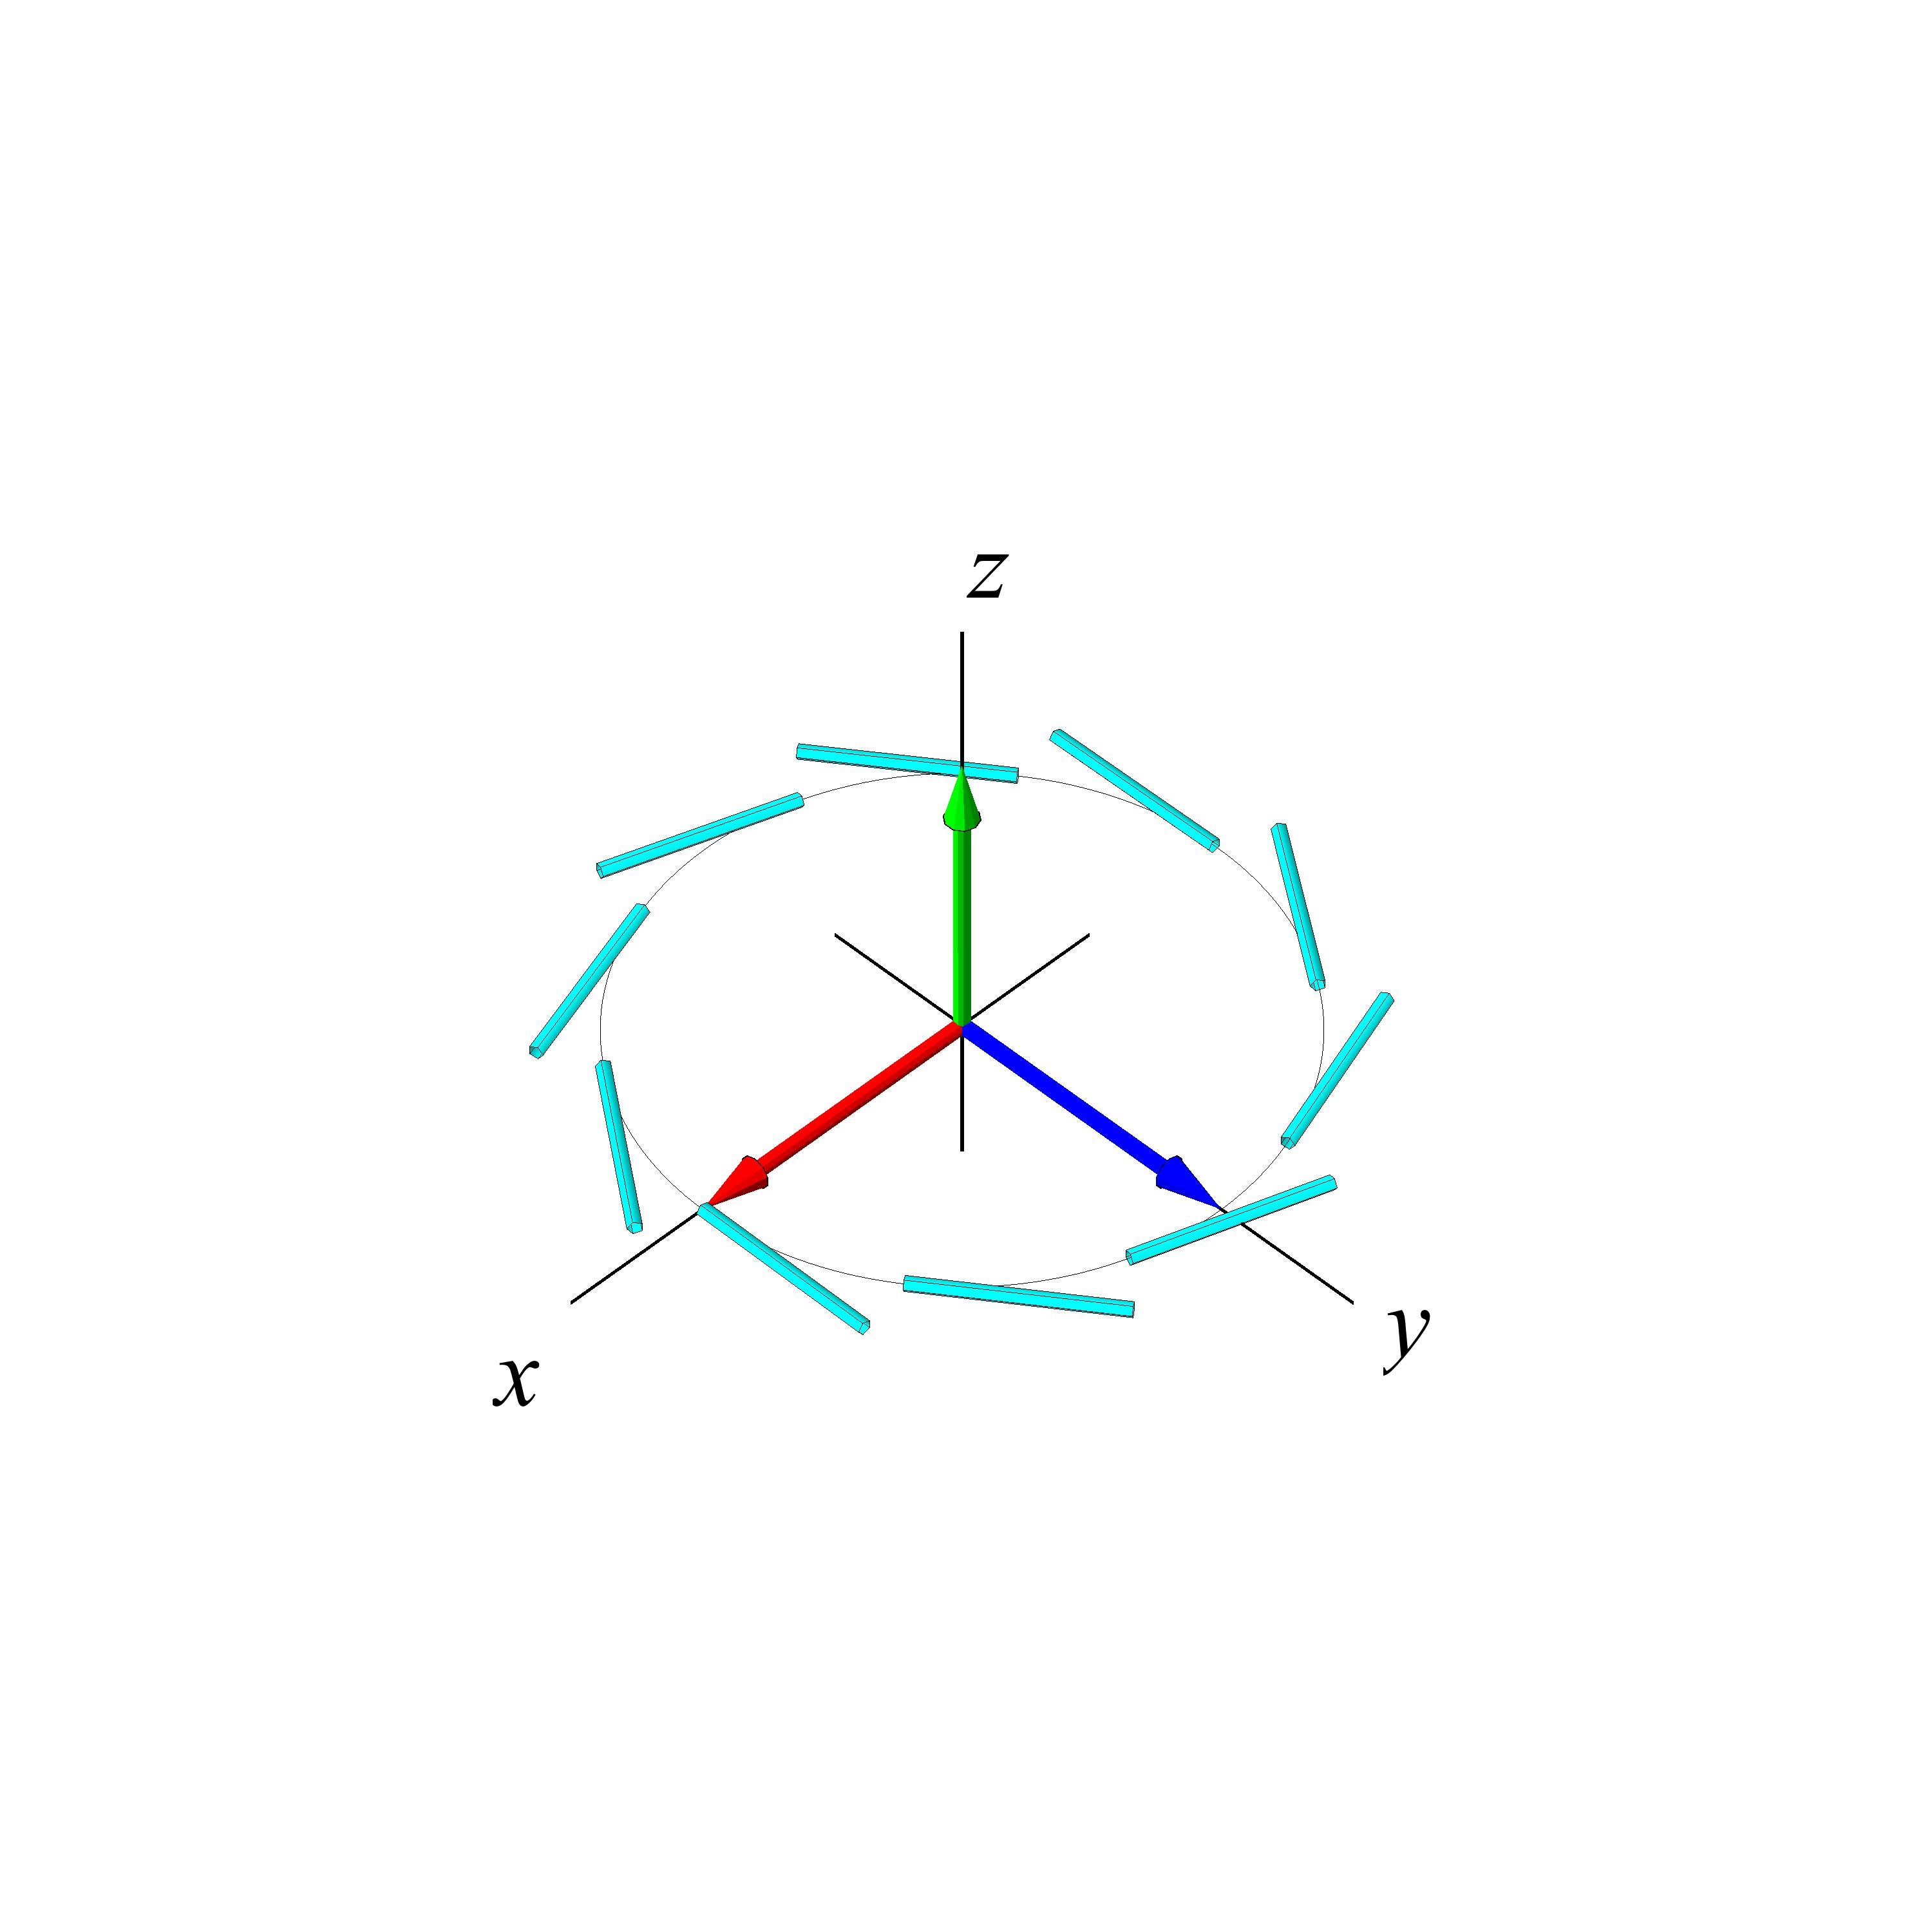
\includegraphics[height=55mm]{FIGS/plotC1app}\,\,\,\,\,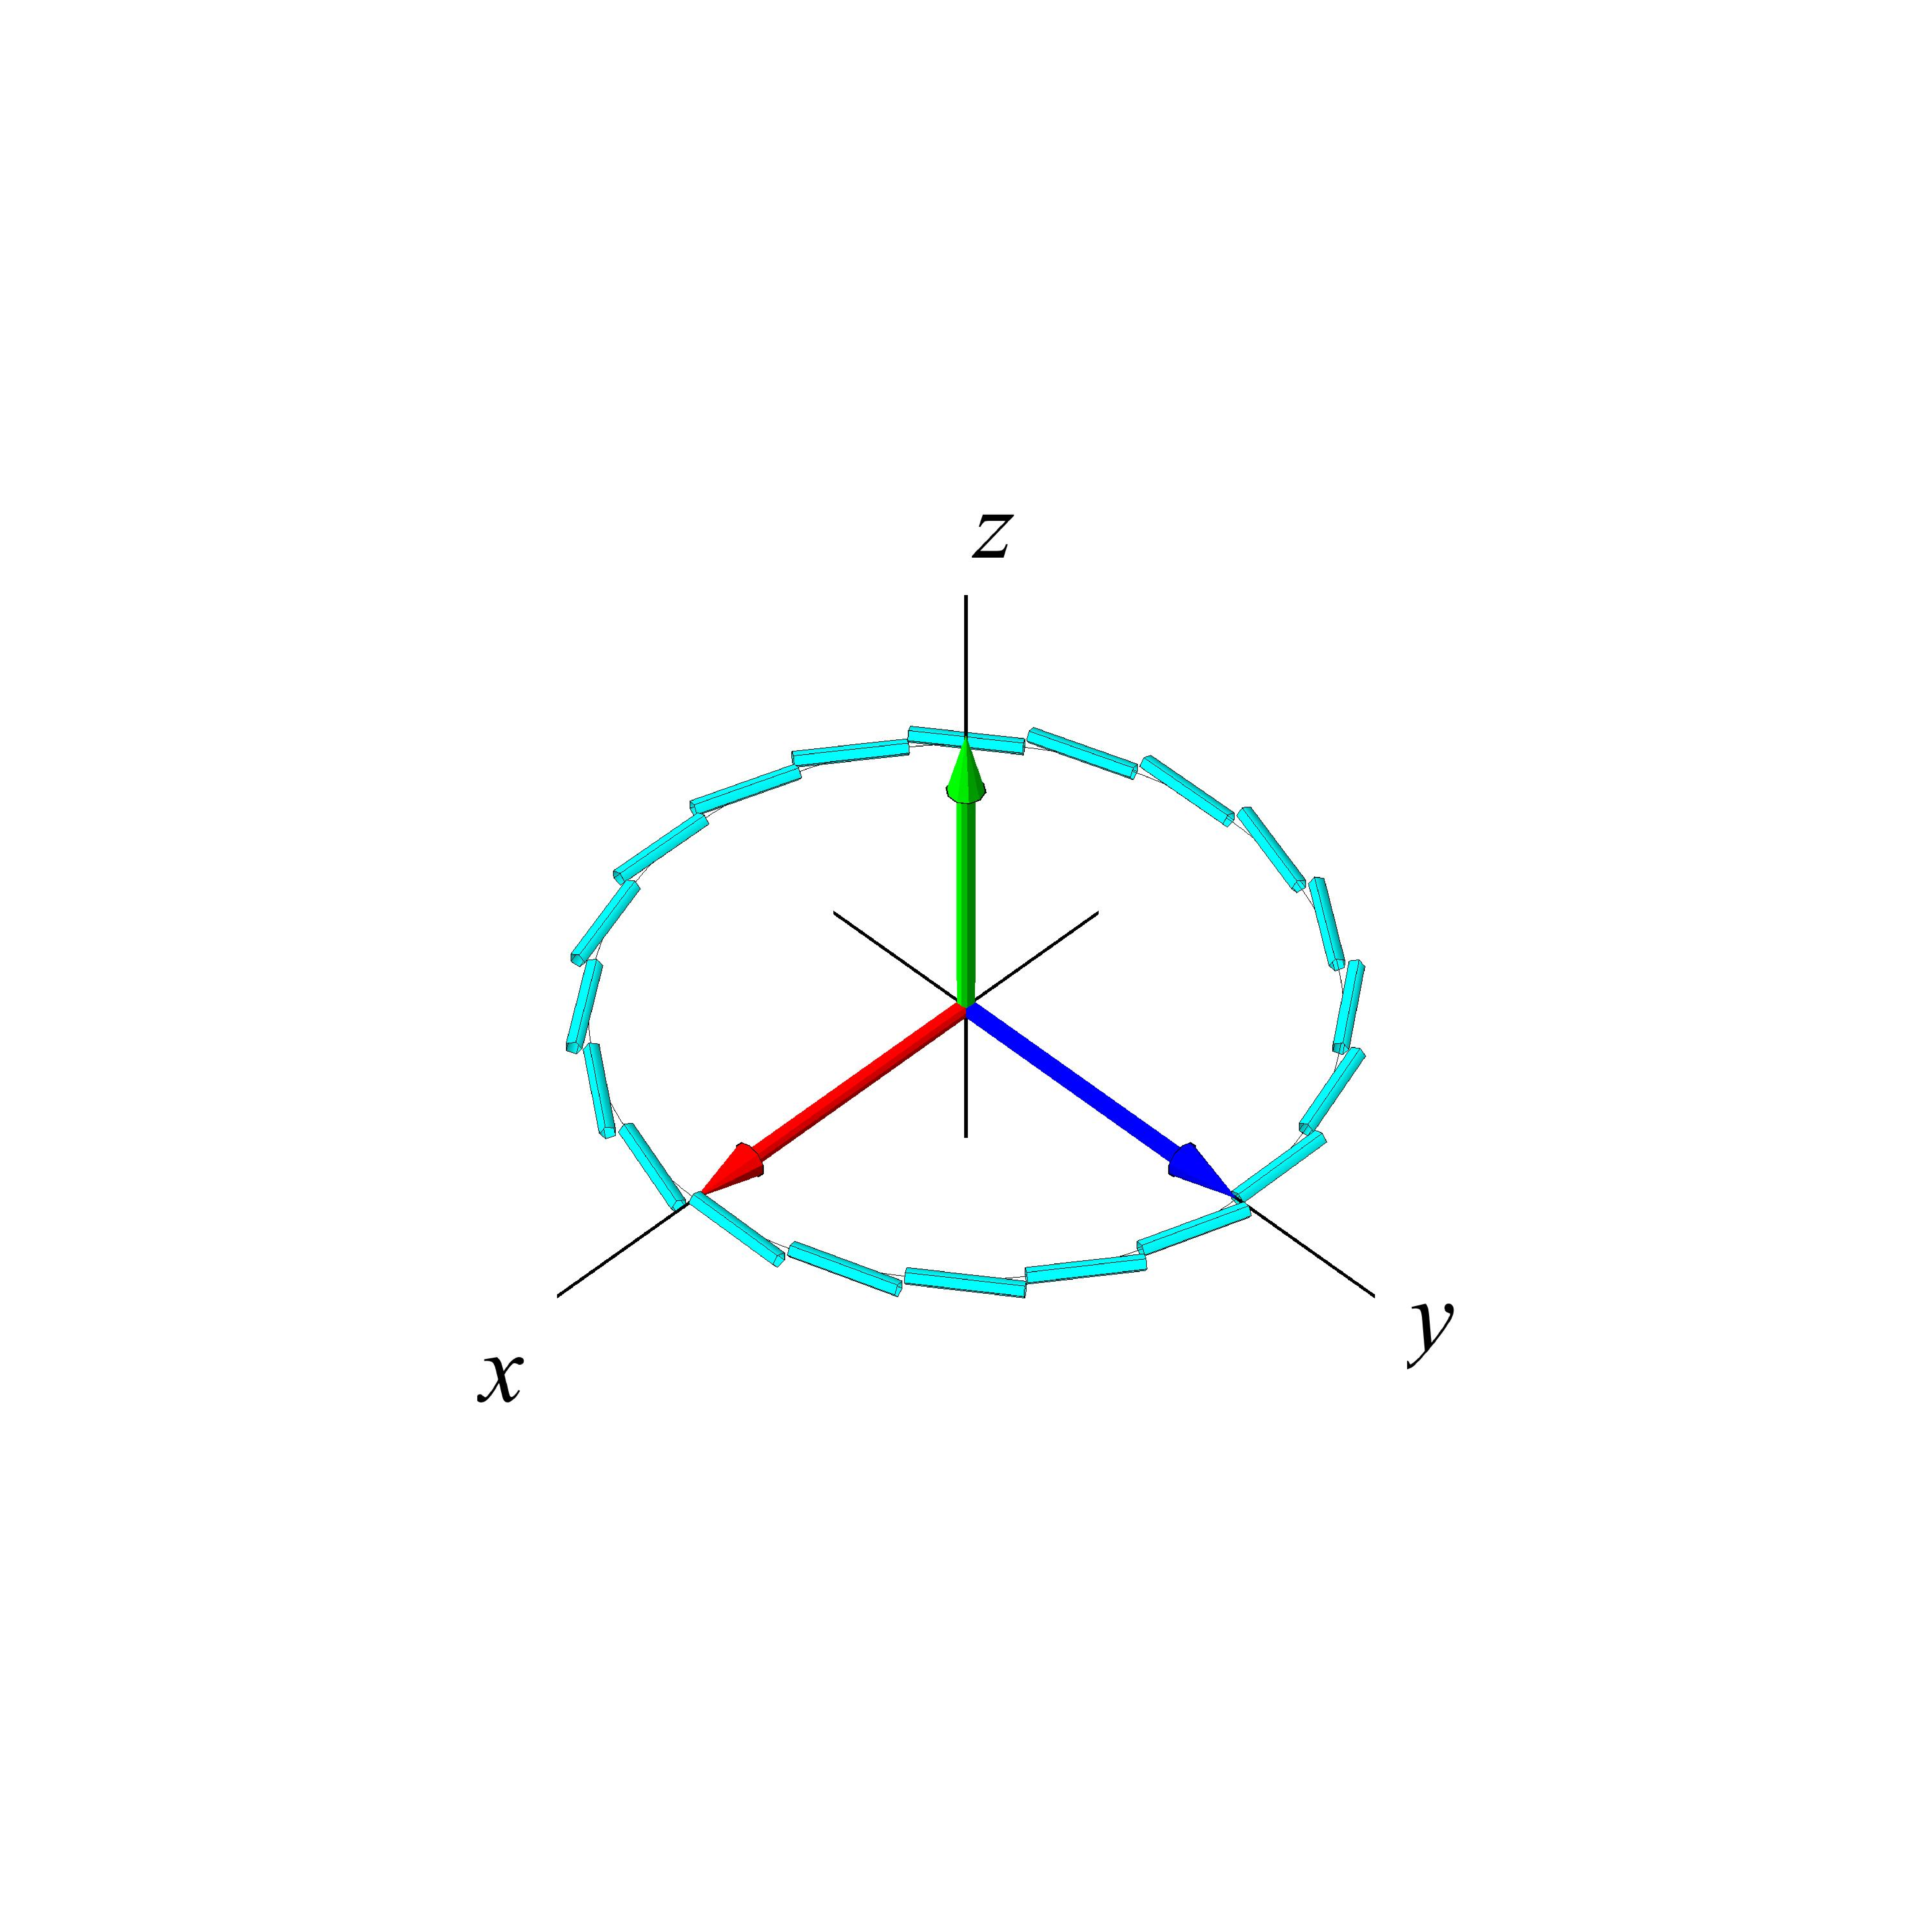
\includegraphics[height=55mm]{FIGS/plotC2app}\,\,\,\,\,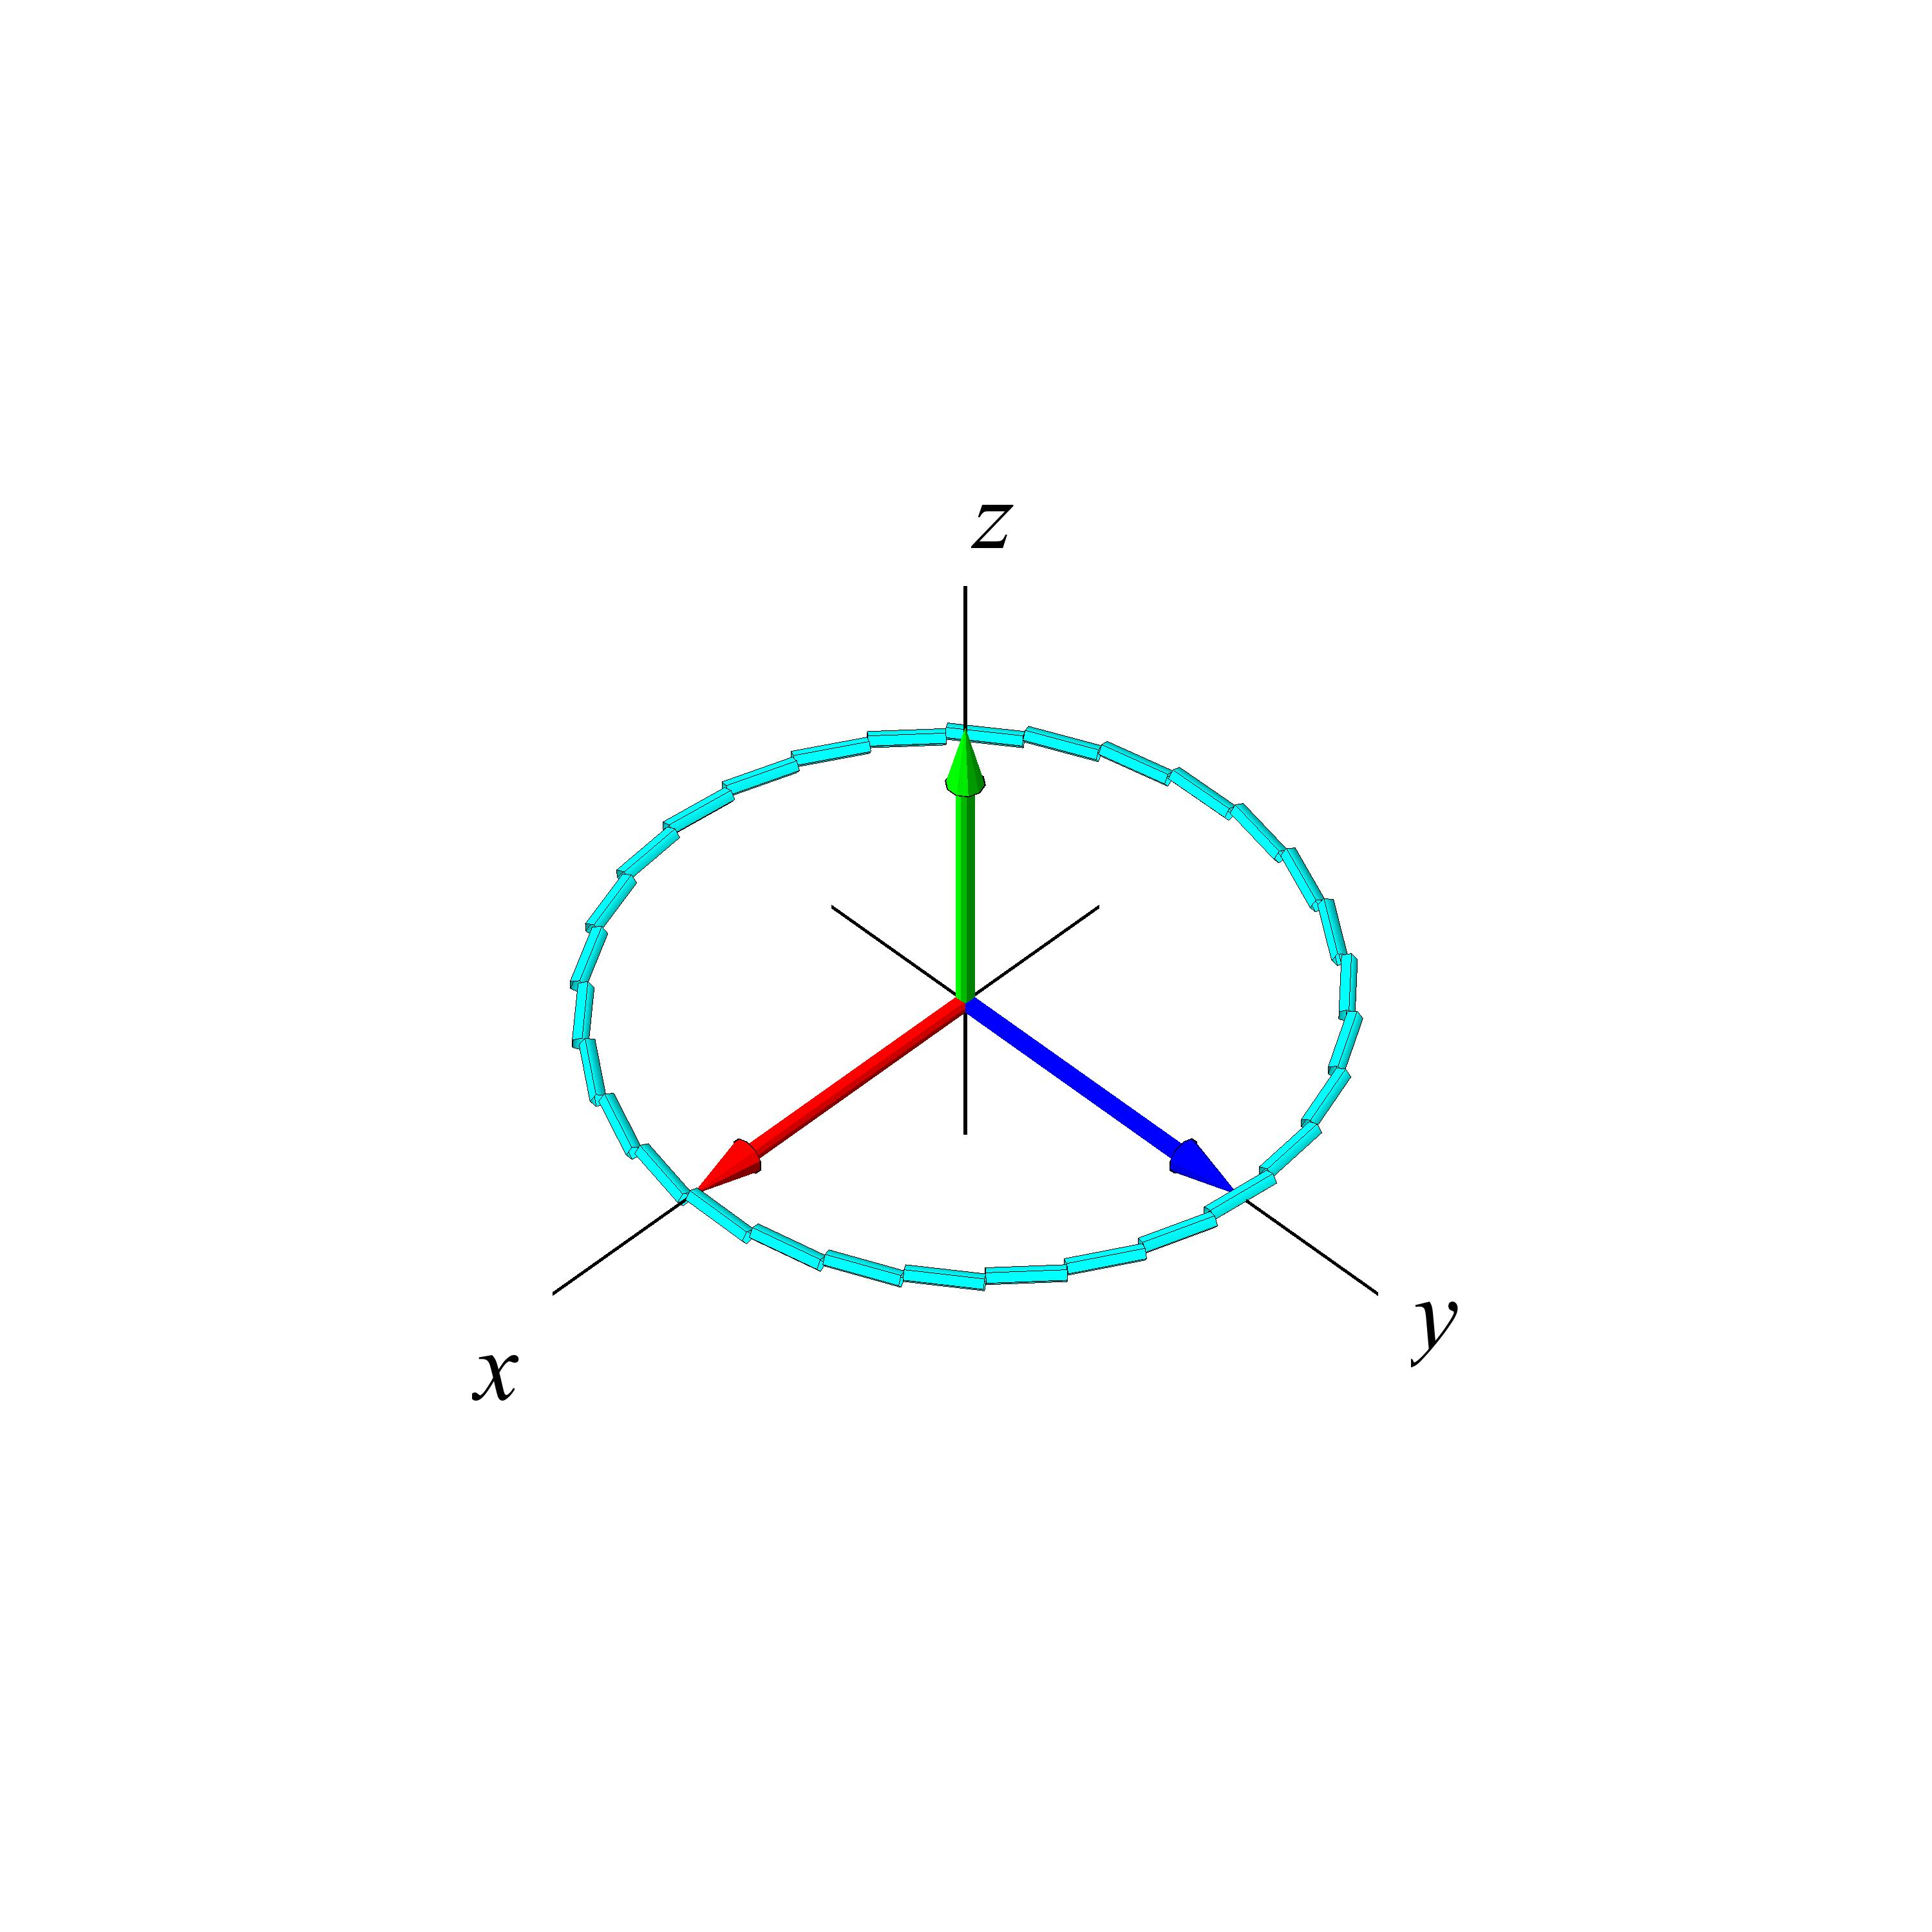
\includegraphics[height=55mm]{FIGS/plotC3app}}
\begin{center}
\caption{ \small{Kurven ${\bf r}(u) \, = \,
\left(\cos(2\pi u), \,\sin(2\pi u),\, 0\right),
\, \, u \, \in [-1, 1]\, ,$ med henholdsvis 10, 20, og
30 approksimerende linjestykker. Det er
rimeligt at definere længden af kurven som den
totale længde af de approksimerende linjestykker
i den grænse hvor antallet af linjestykker går
mod uendelig.}} \label{figCircApprox123}
\end{center}
\end{figure}




\begin{figure}[ht]
\centerline{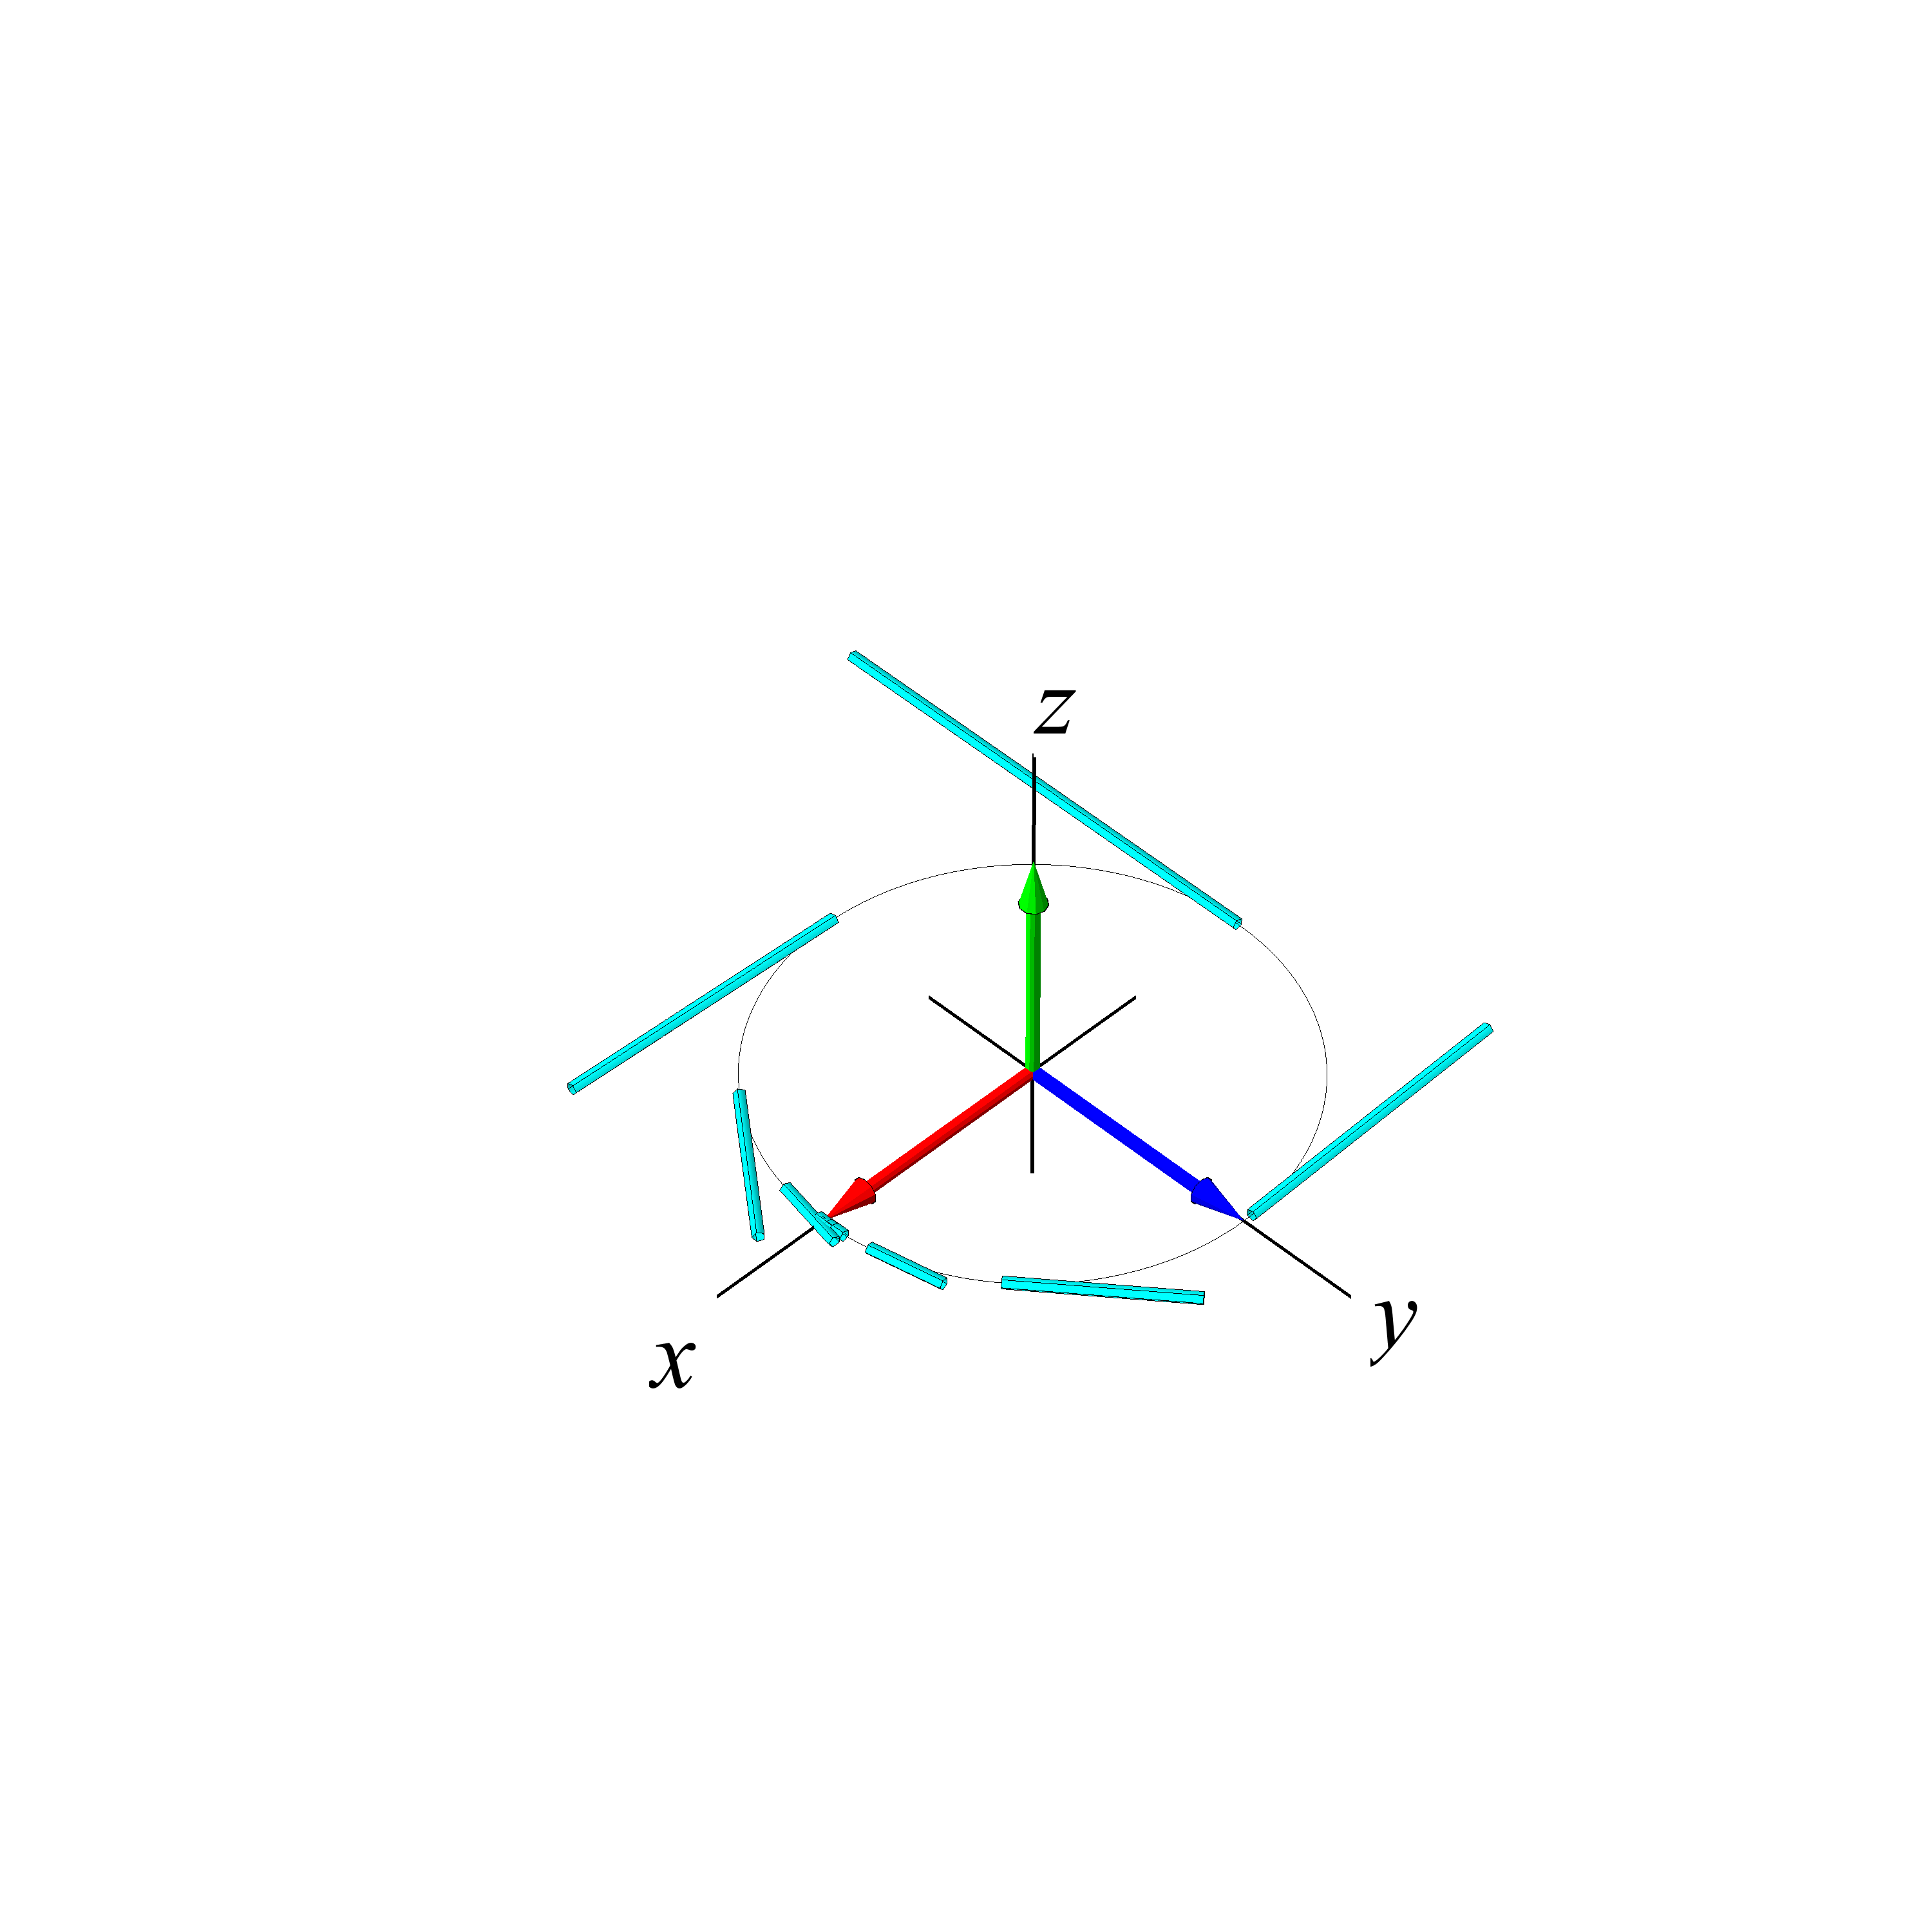
\includegraphics[height=55mm]{FIGS/plotCtredjeapp1}\,\,\,\,\,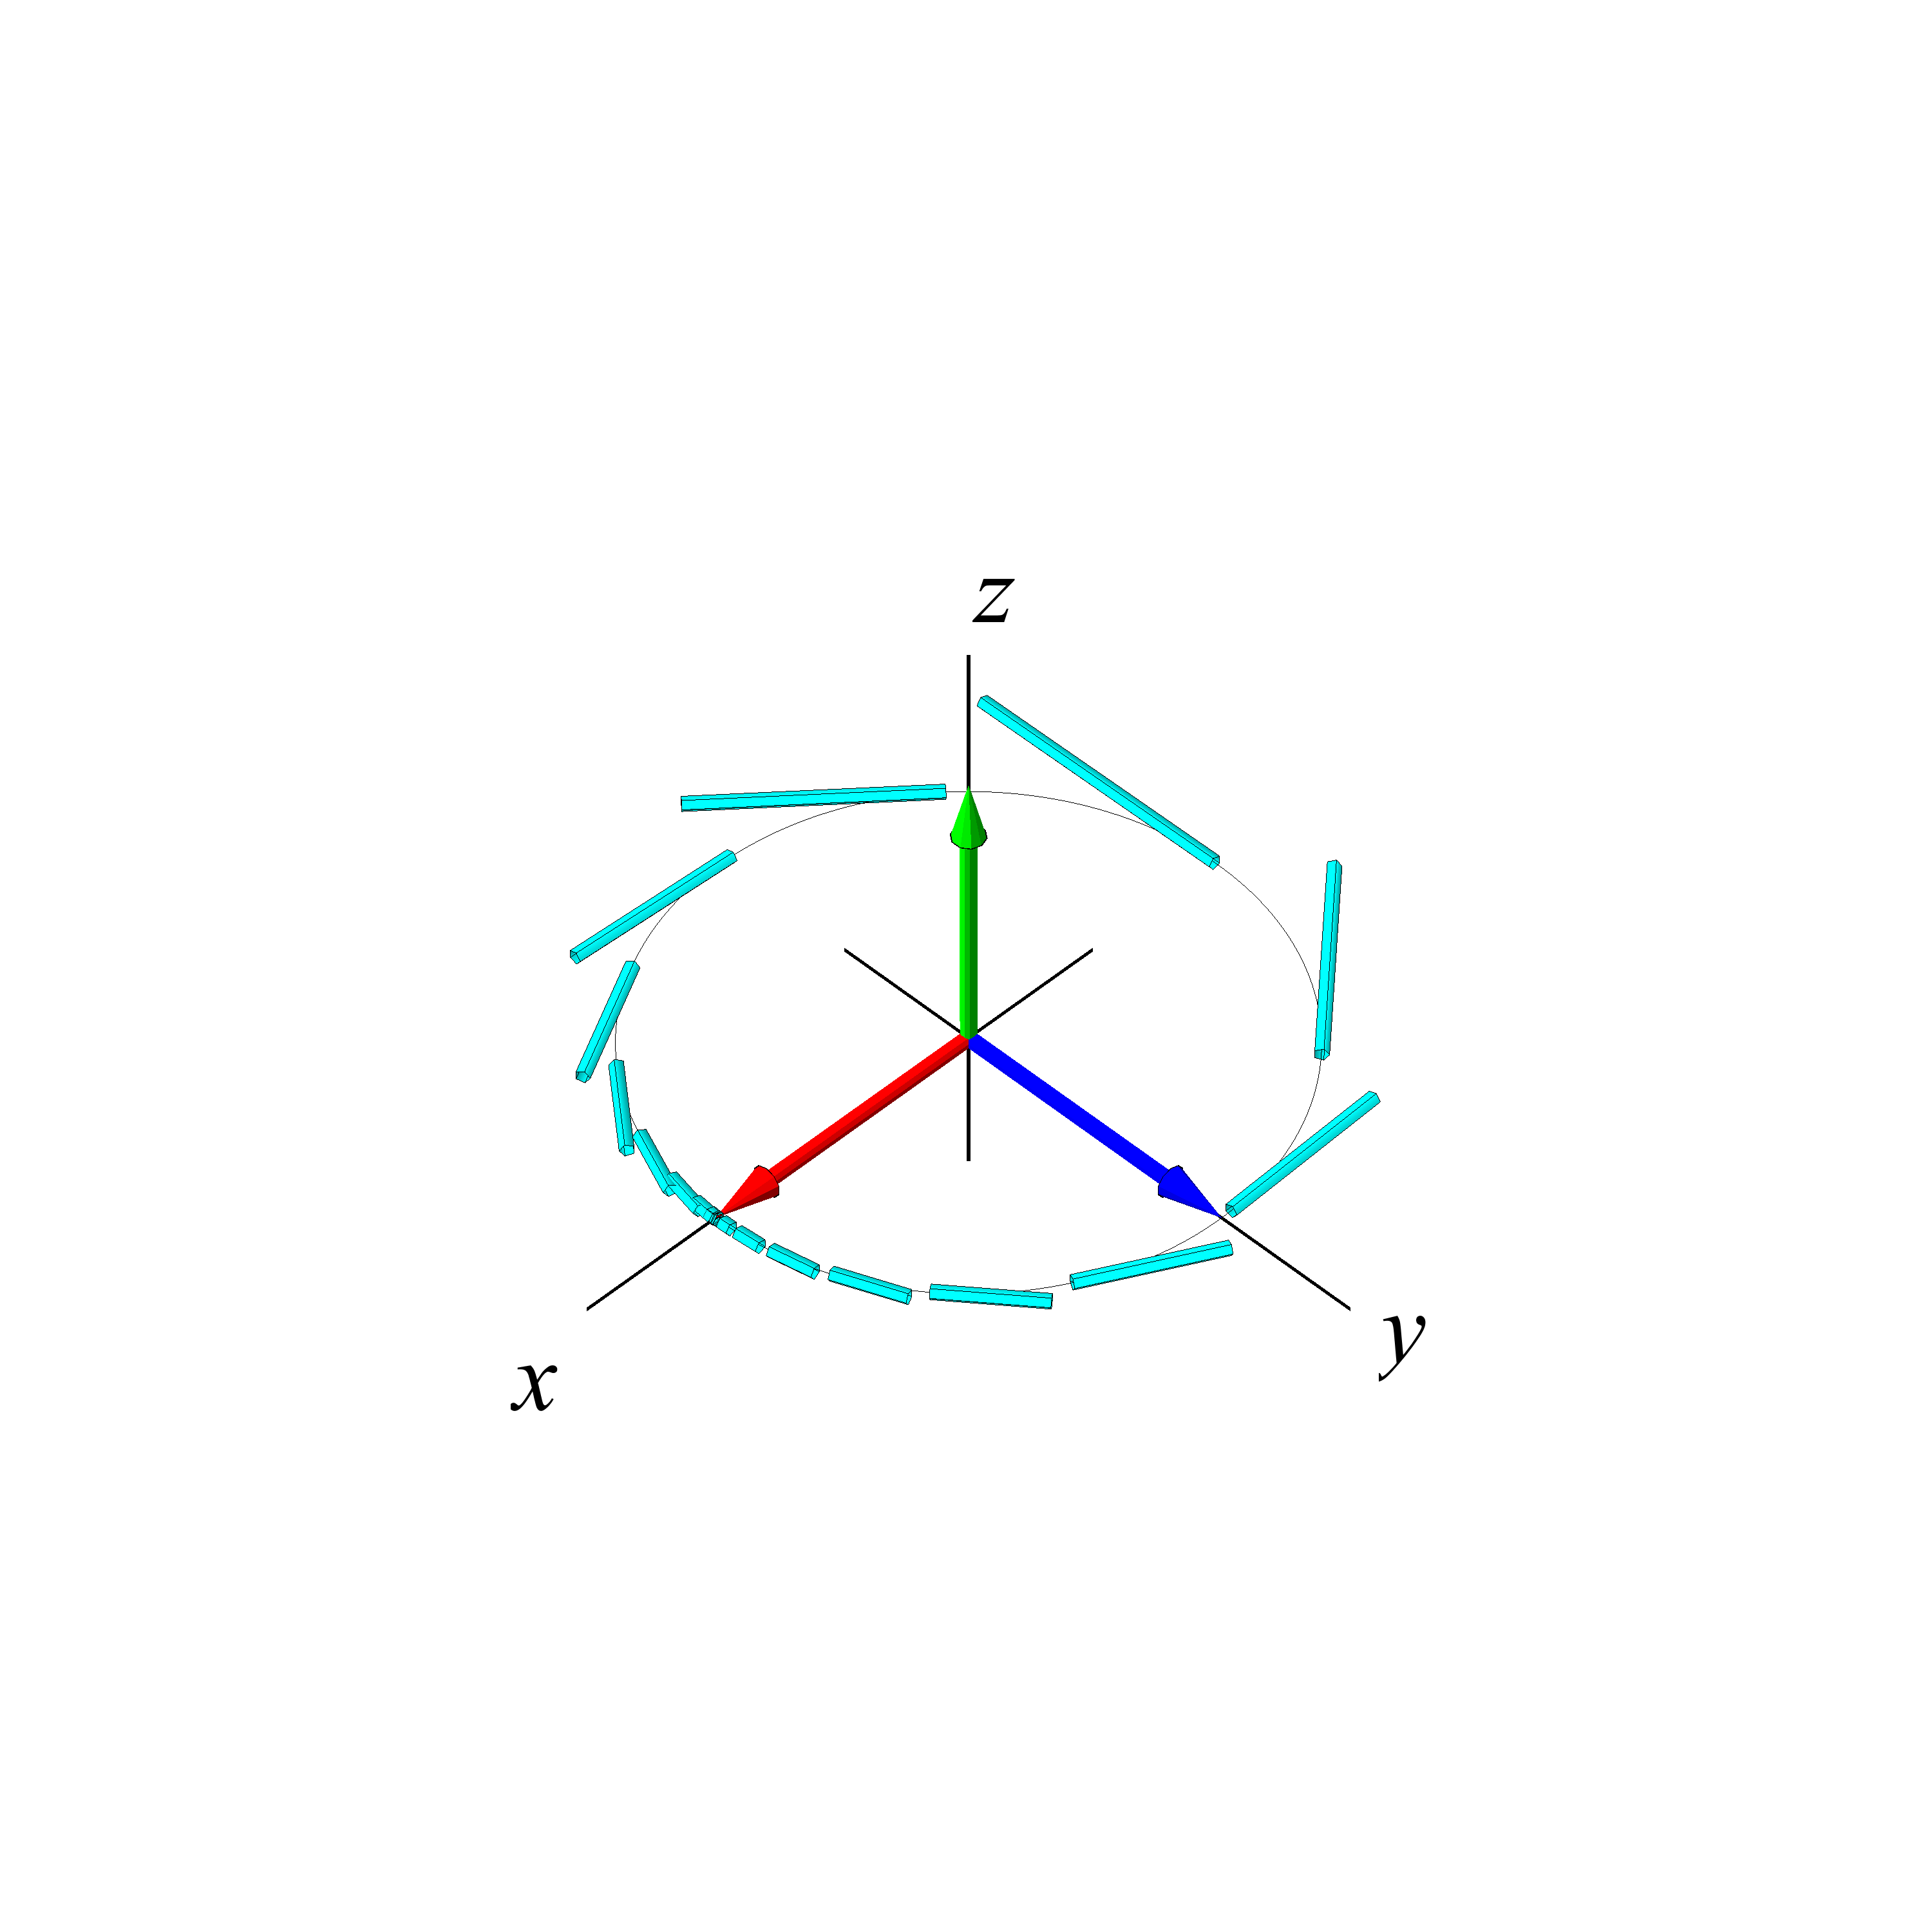
\includegraphics[height=55mm]{FIGS/plotCtredjeapp2}\,\,\,\,\,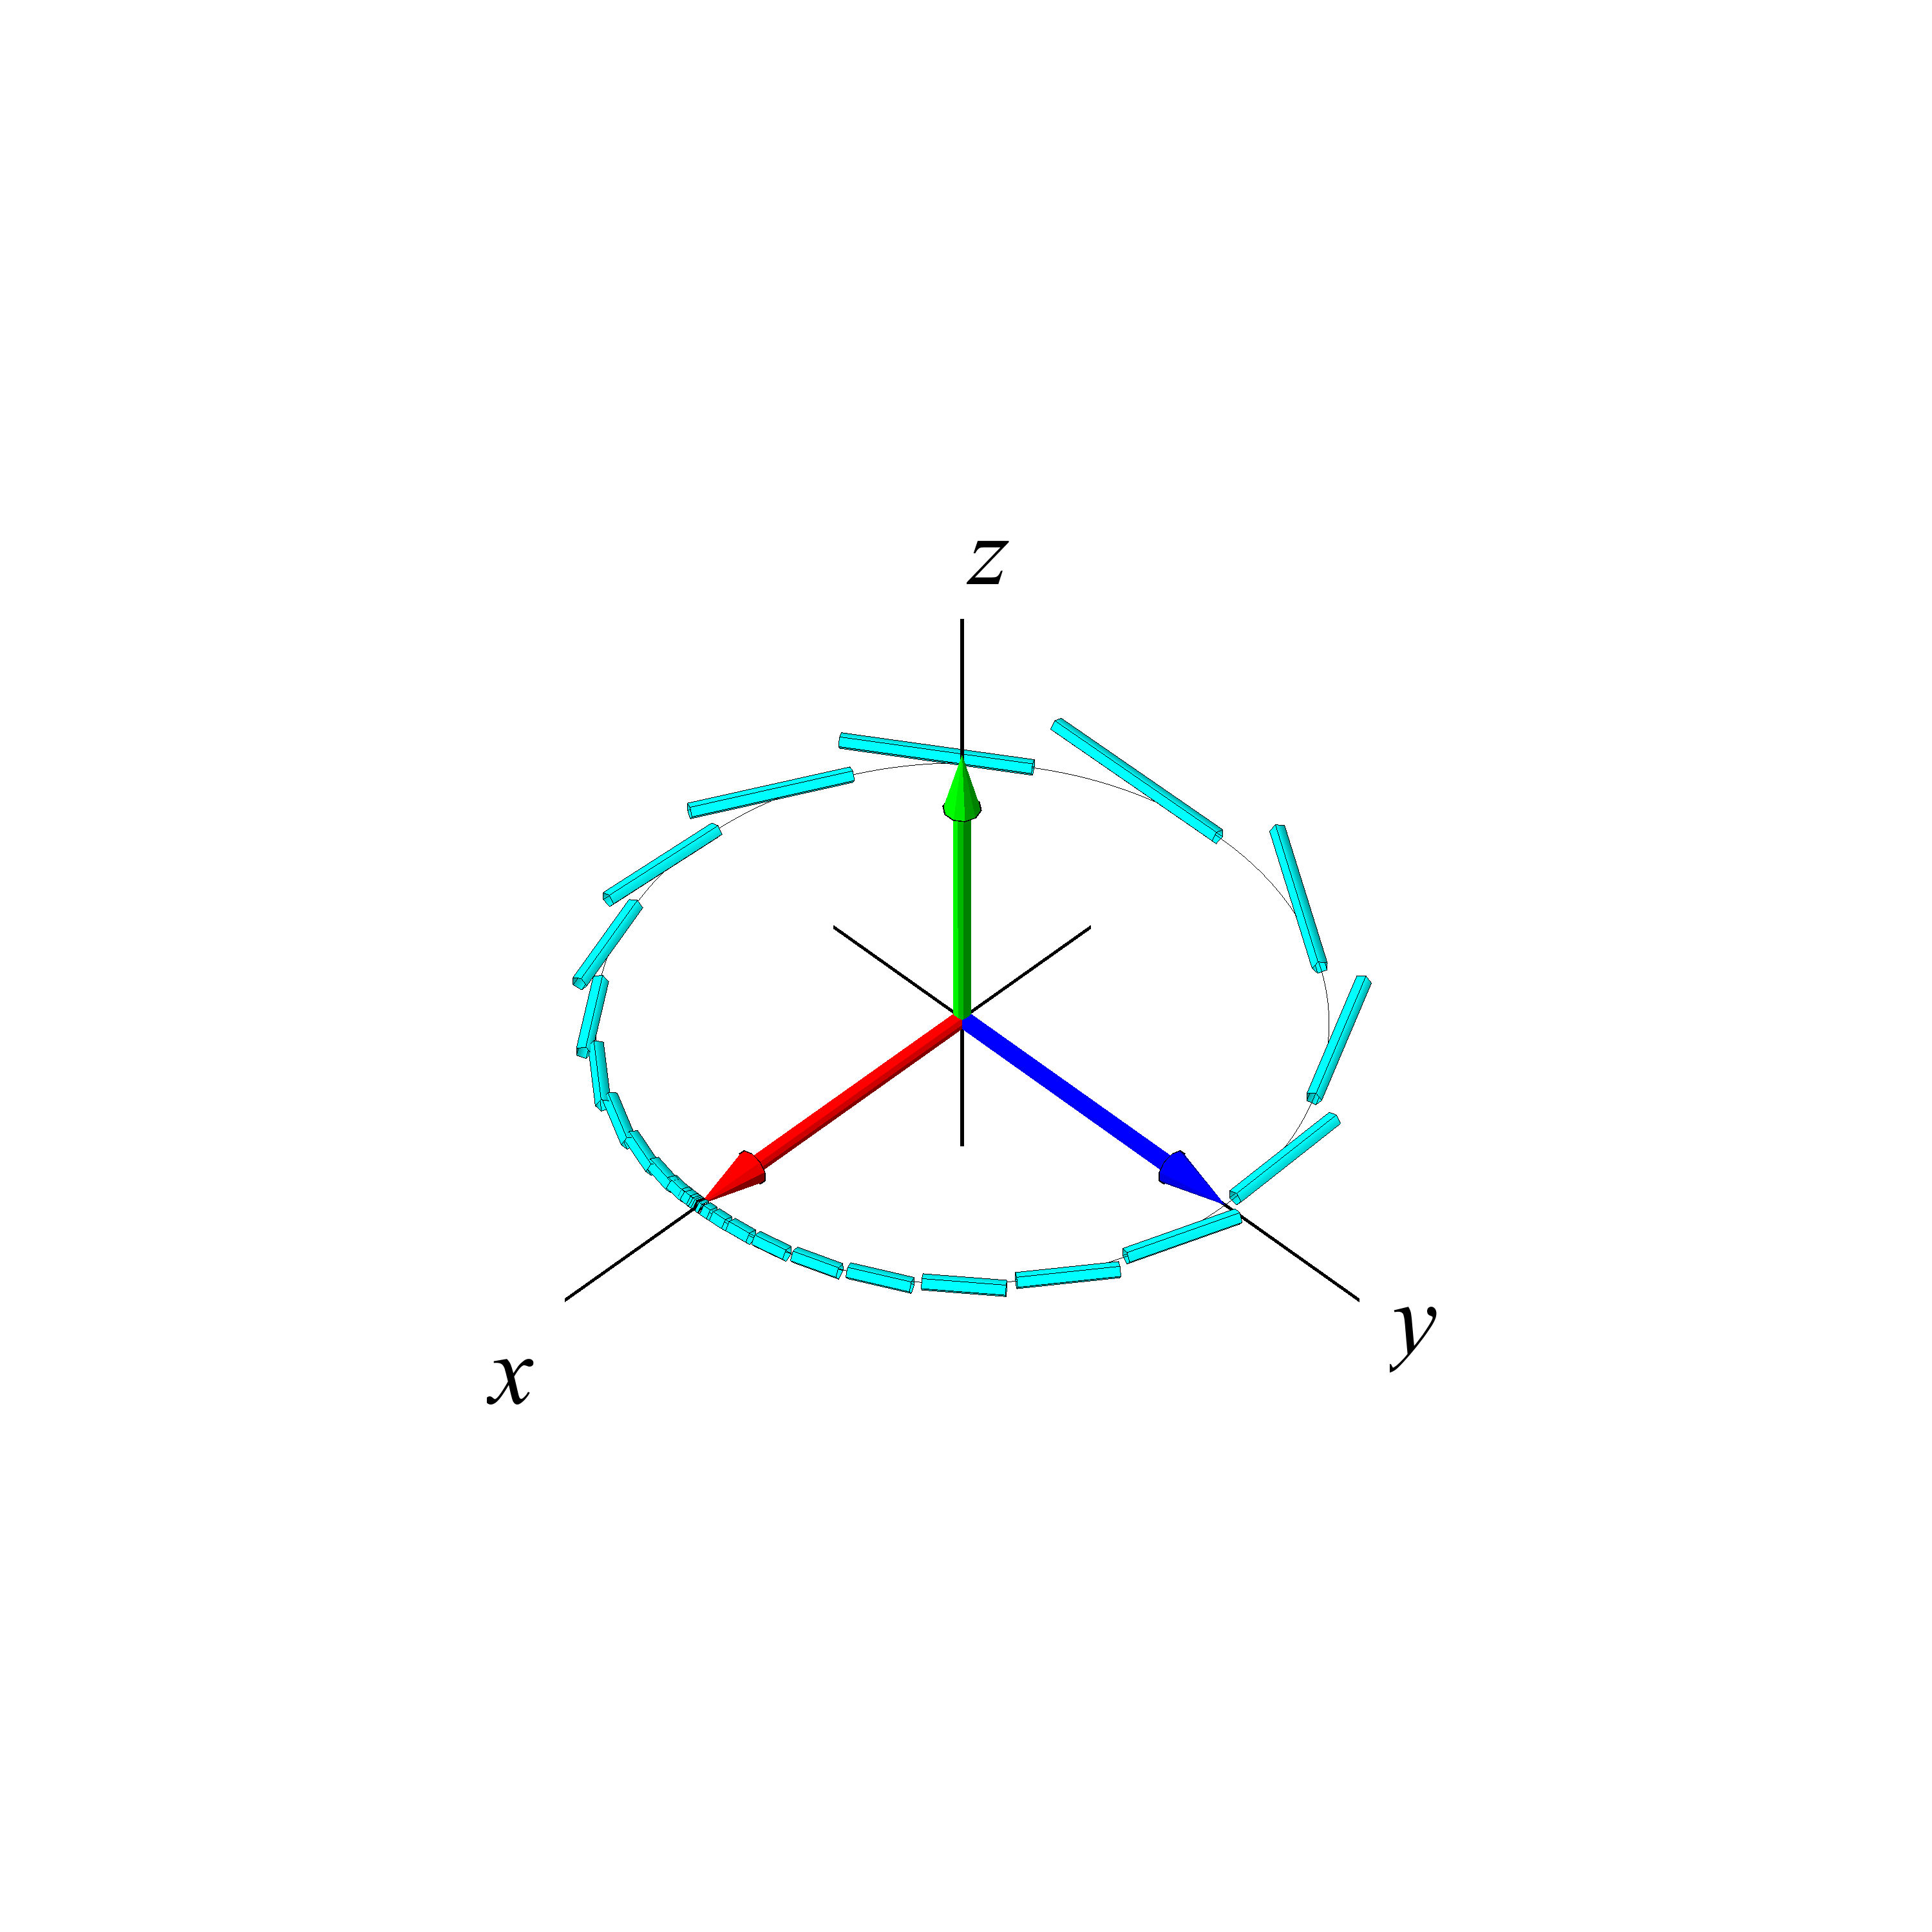
\includegraphics[height=55mm]{FIGS/plotCtredjeapp3}}
\begin{center}
\caption{\small{ Kurven ${\bf r}(u) \, = \,
\left(\cos(2\pi u^{3}), \,\sin(2\pi u^{3}),\,
0\right), \, \, u \, \in [-1, 1]\, ,$ med
henholdsvis 30, 60 og 100 approksimerende
linjestykker. Det er stadig rimeligt at definere
længden af kurven som den totale længde af de
approksimerende linjestykker i den grænse hvor
antallet af approksimerende linjestykker går mod
uendelig.}} \label{figcircAppB123}
\end{center}
\end{figure}


%%%%%%%%%%%%%%%%%%%%%%%%%%%%%%%%%%%%%%%%%%%%%%%%%%%
%%%%%%%%%%%%%%%%%%%%%%%%%%%%%%%%%%%%%%%%%%%%%%%%%%%
%%%%%%%%%%%%%%%%%%%%%%%%%%%%%%%%%%%%%%%%%%%%%%%%%%%




\subsubsection{Masse, vægten af en kurve med massetæthed}\label{subsecMasseKurve}
Hvis vi antager, at
hvert enkelt linjestykke i (\ref{eqApp}) tildeles en konstant
massetæthed givet ved værdien af funktionen $f(x,y,z)$ i
linjestykkets kontaktpunkt med kurven, så får vi massen af det $i$'te
linjestykke:
$$
\Delta \M_{i} \, = \, f(x(u_{i}), y(u_{i}), z(u_{i}))\, | {\bf
r}'(u_{i}) | \cdot\delta_{u} \, = \, f({\bf{r}}(u_{i}))\, | {\bf
r}'(u_{i}) | \cdot\delta_{u}\quad .
$$
Den totale masse af hele systemet af linjestykker er derfor
følgende, som er en god approksimation til massen af hele kurven,
når kurven tildeles massetætheden $f({\bf r}(u))$ på stedet ${\bf
r}(u)$ :
\begin{equation}
\M_{\app}(n) \, = \,   \sum_{i=1}^{n} \Delta \M_{i} \, = \,
\sum_{i=1}^{n}f({\bf r}(u_{i}))\, | {\bf r}'(u_{i}) | \cdot \delta_{u}
\quad .
\end{equation}

Dette er igen en integralsum, men nu for den kontinuerte funktion
$f({\bf r}(u))\, | {\bf r}'(u) | $ over intervallet $\,[a,
b]\,$. Vi får altså i grænsen, hvor $n$ går mod uendelig:
\begin{equation}
\M_{\app}(n)\, \to \, \M \, = \, \int_{a}^{b}f({\bf r}(u)) | {\bf
r}'(u) | \,du \quad \text{for} \quad n \to \infty \quad.
\end{equation}

Dermed har vi motiveret definitionen af massen af en kurve med
massetætheden $f({\bf r}(u))$ (for så vidt denne funktion er
positiv i $\,[a,b]\,$) og dermed den generelle definition af
kurveintegralet, Definition \ref{defKurveInt}.

%%%%%%%%%%%%%%%%%%%%%%%%%%%%%%%%%%%%%%%%%%%%%%%%%%%
%%%%%%%%%%%%%%%%%%%%%%%%%%%%%%%%%%%%%%%%%%%%%%%%%%%
%%%%%%%%%%%%%%%%%%%%%%%%%%%%%%%%%%%%%%%%%%%%%%%%%%%
%%%%%%%%%%%%%%%%%%%%%%%%%%%%%%%%%%%%%%%%%%%%%%%%%%%
%%%%%%%%%%%%%%%%%%%%%%%%%%%%%%%%%%%%%%%%%%%%%%%%%%%



\section{Planintegraler} \label{secPlanInt}

\begin{figure}[ht]
\centerline{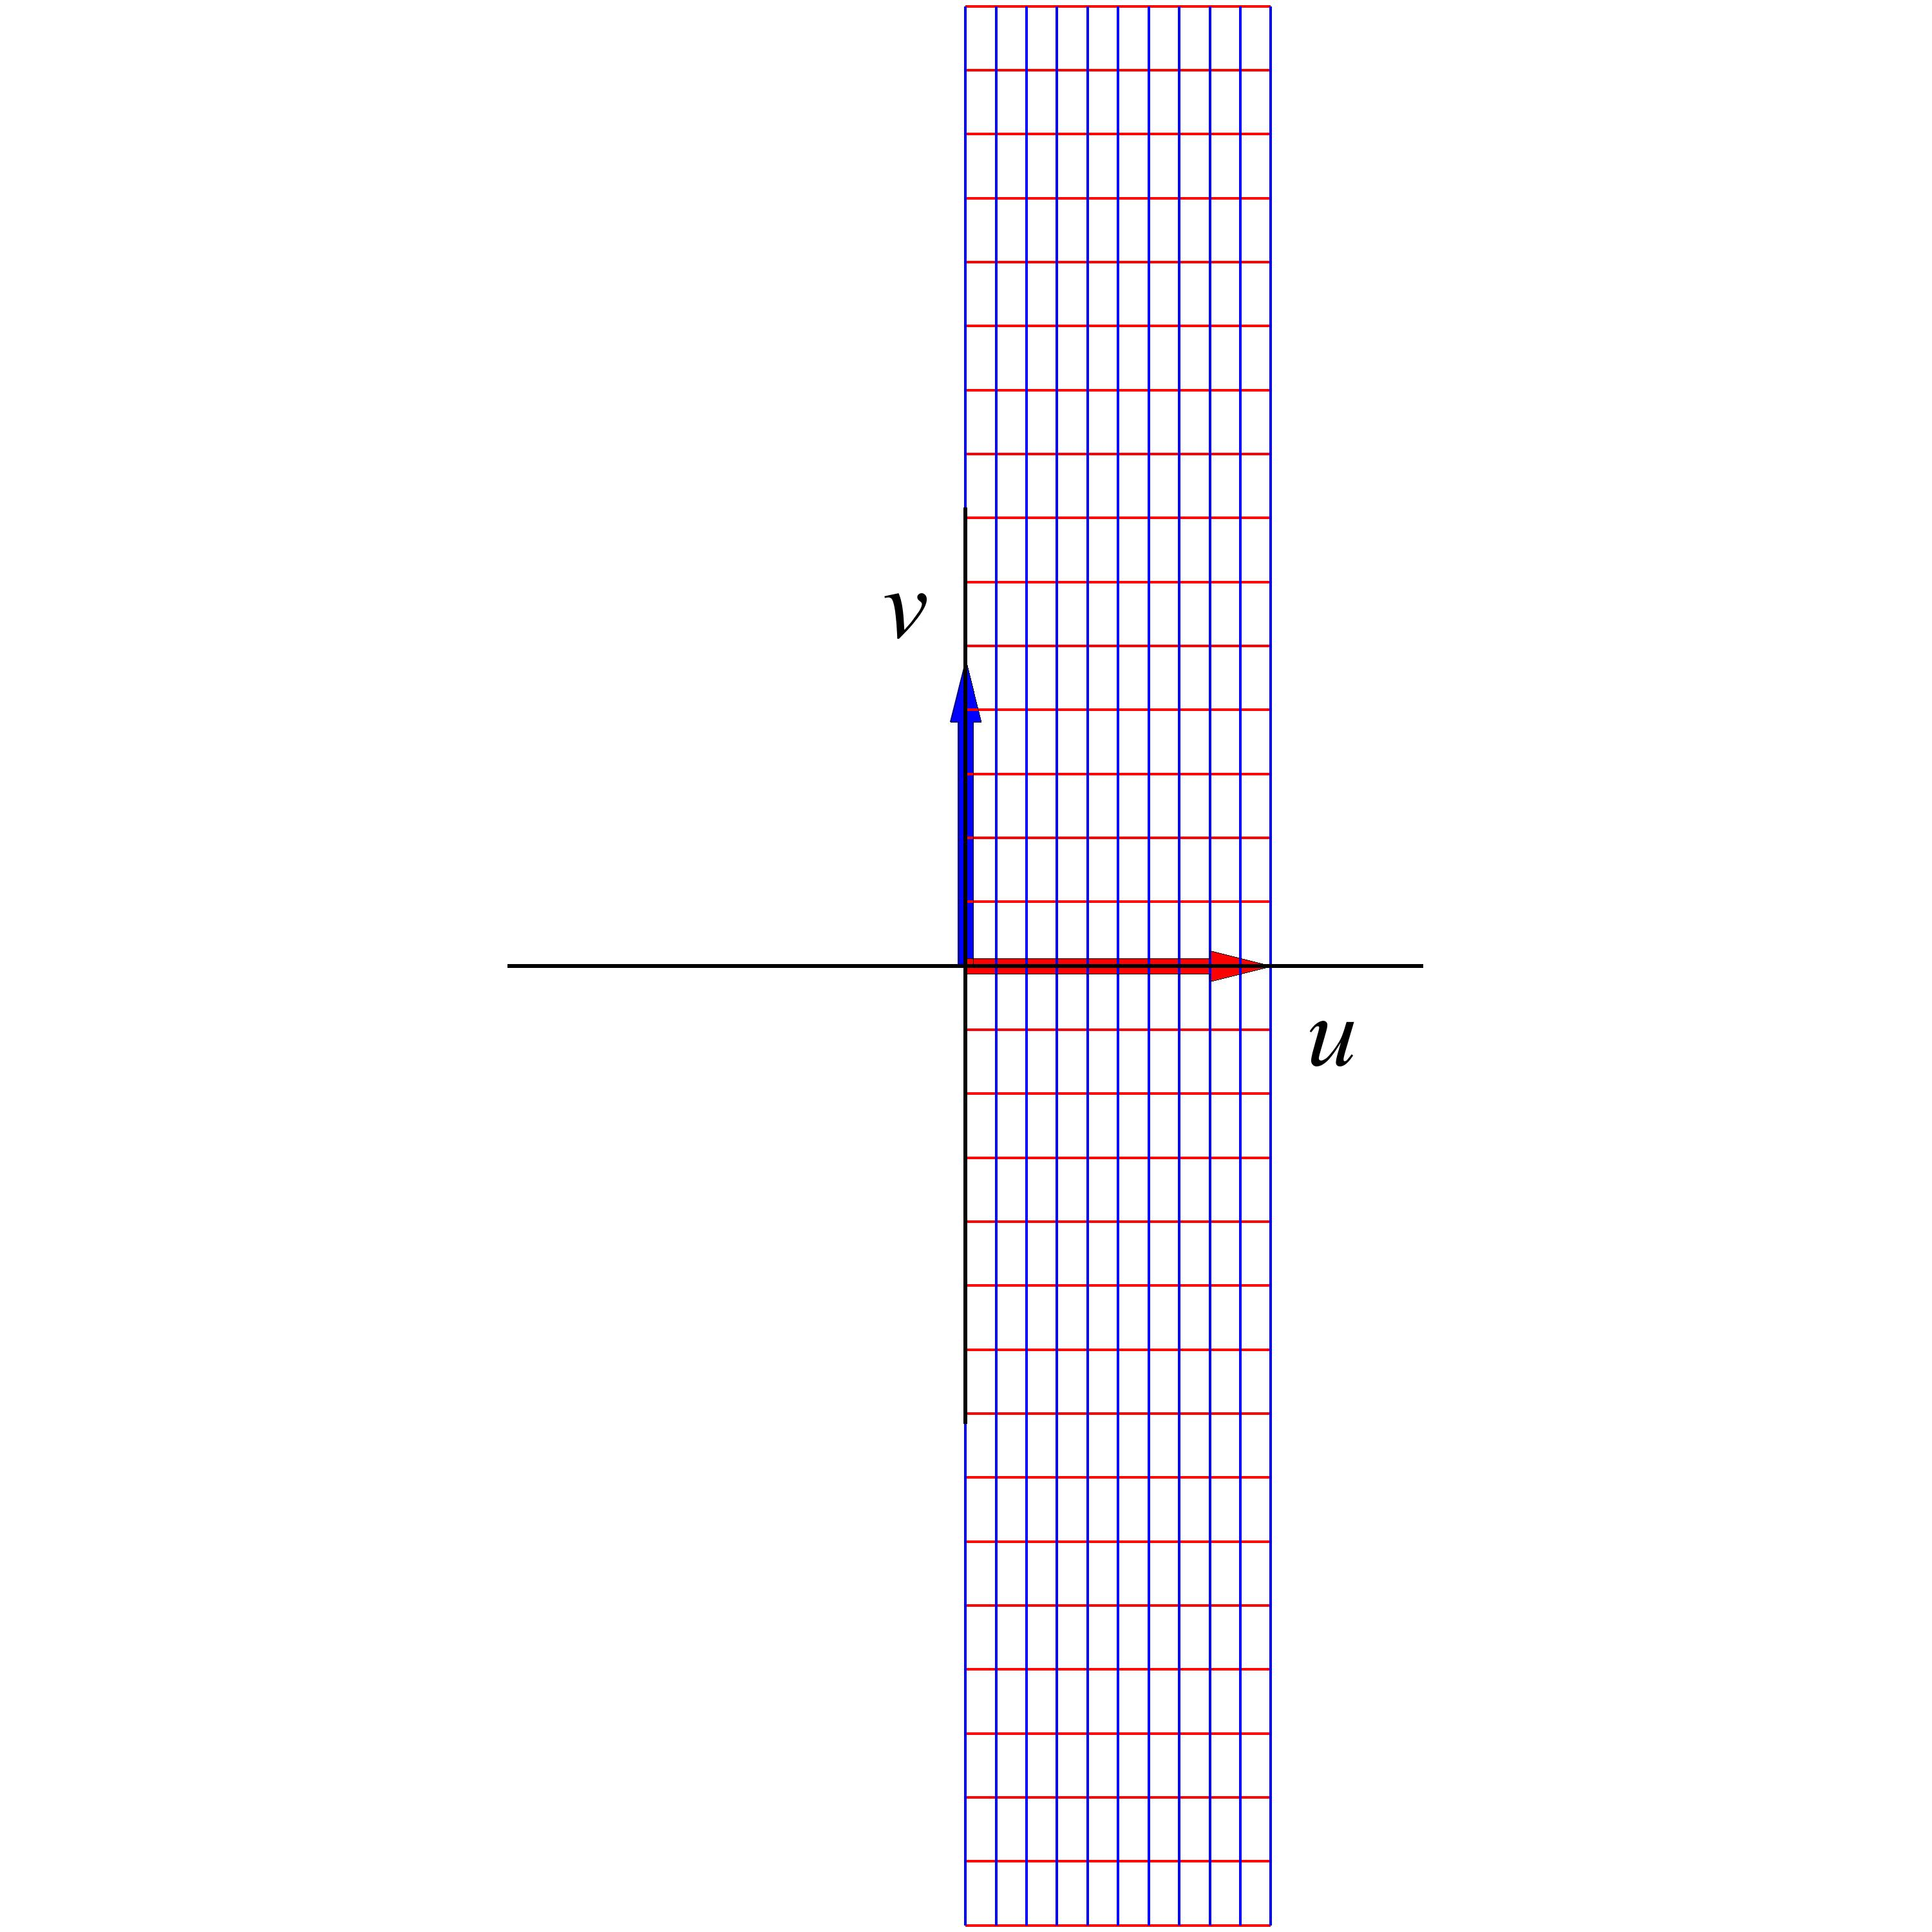
\includegraphics[height=40mm]{FIGS/plotPolarApp1}\,\,\,\,\qquad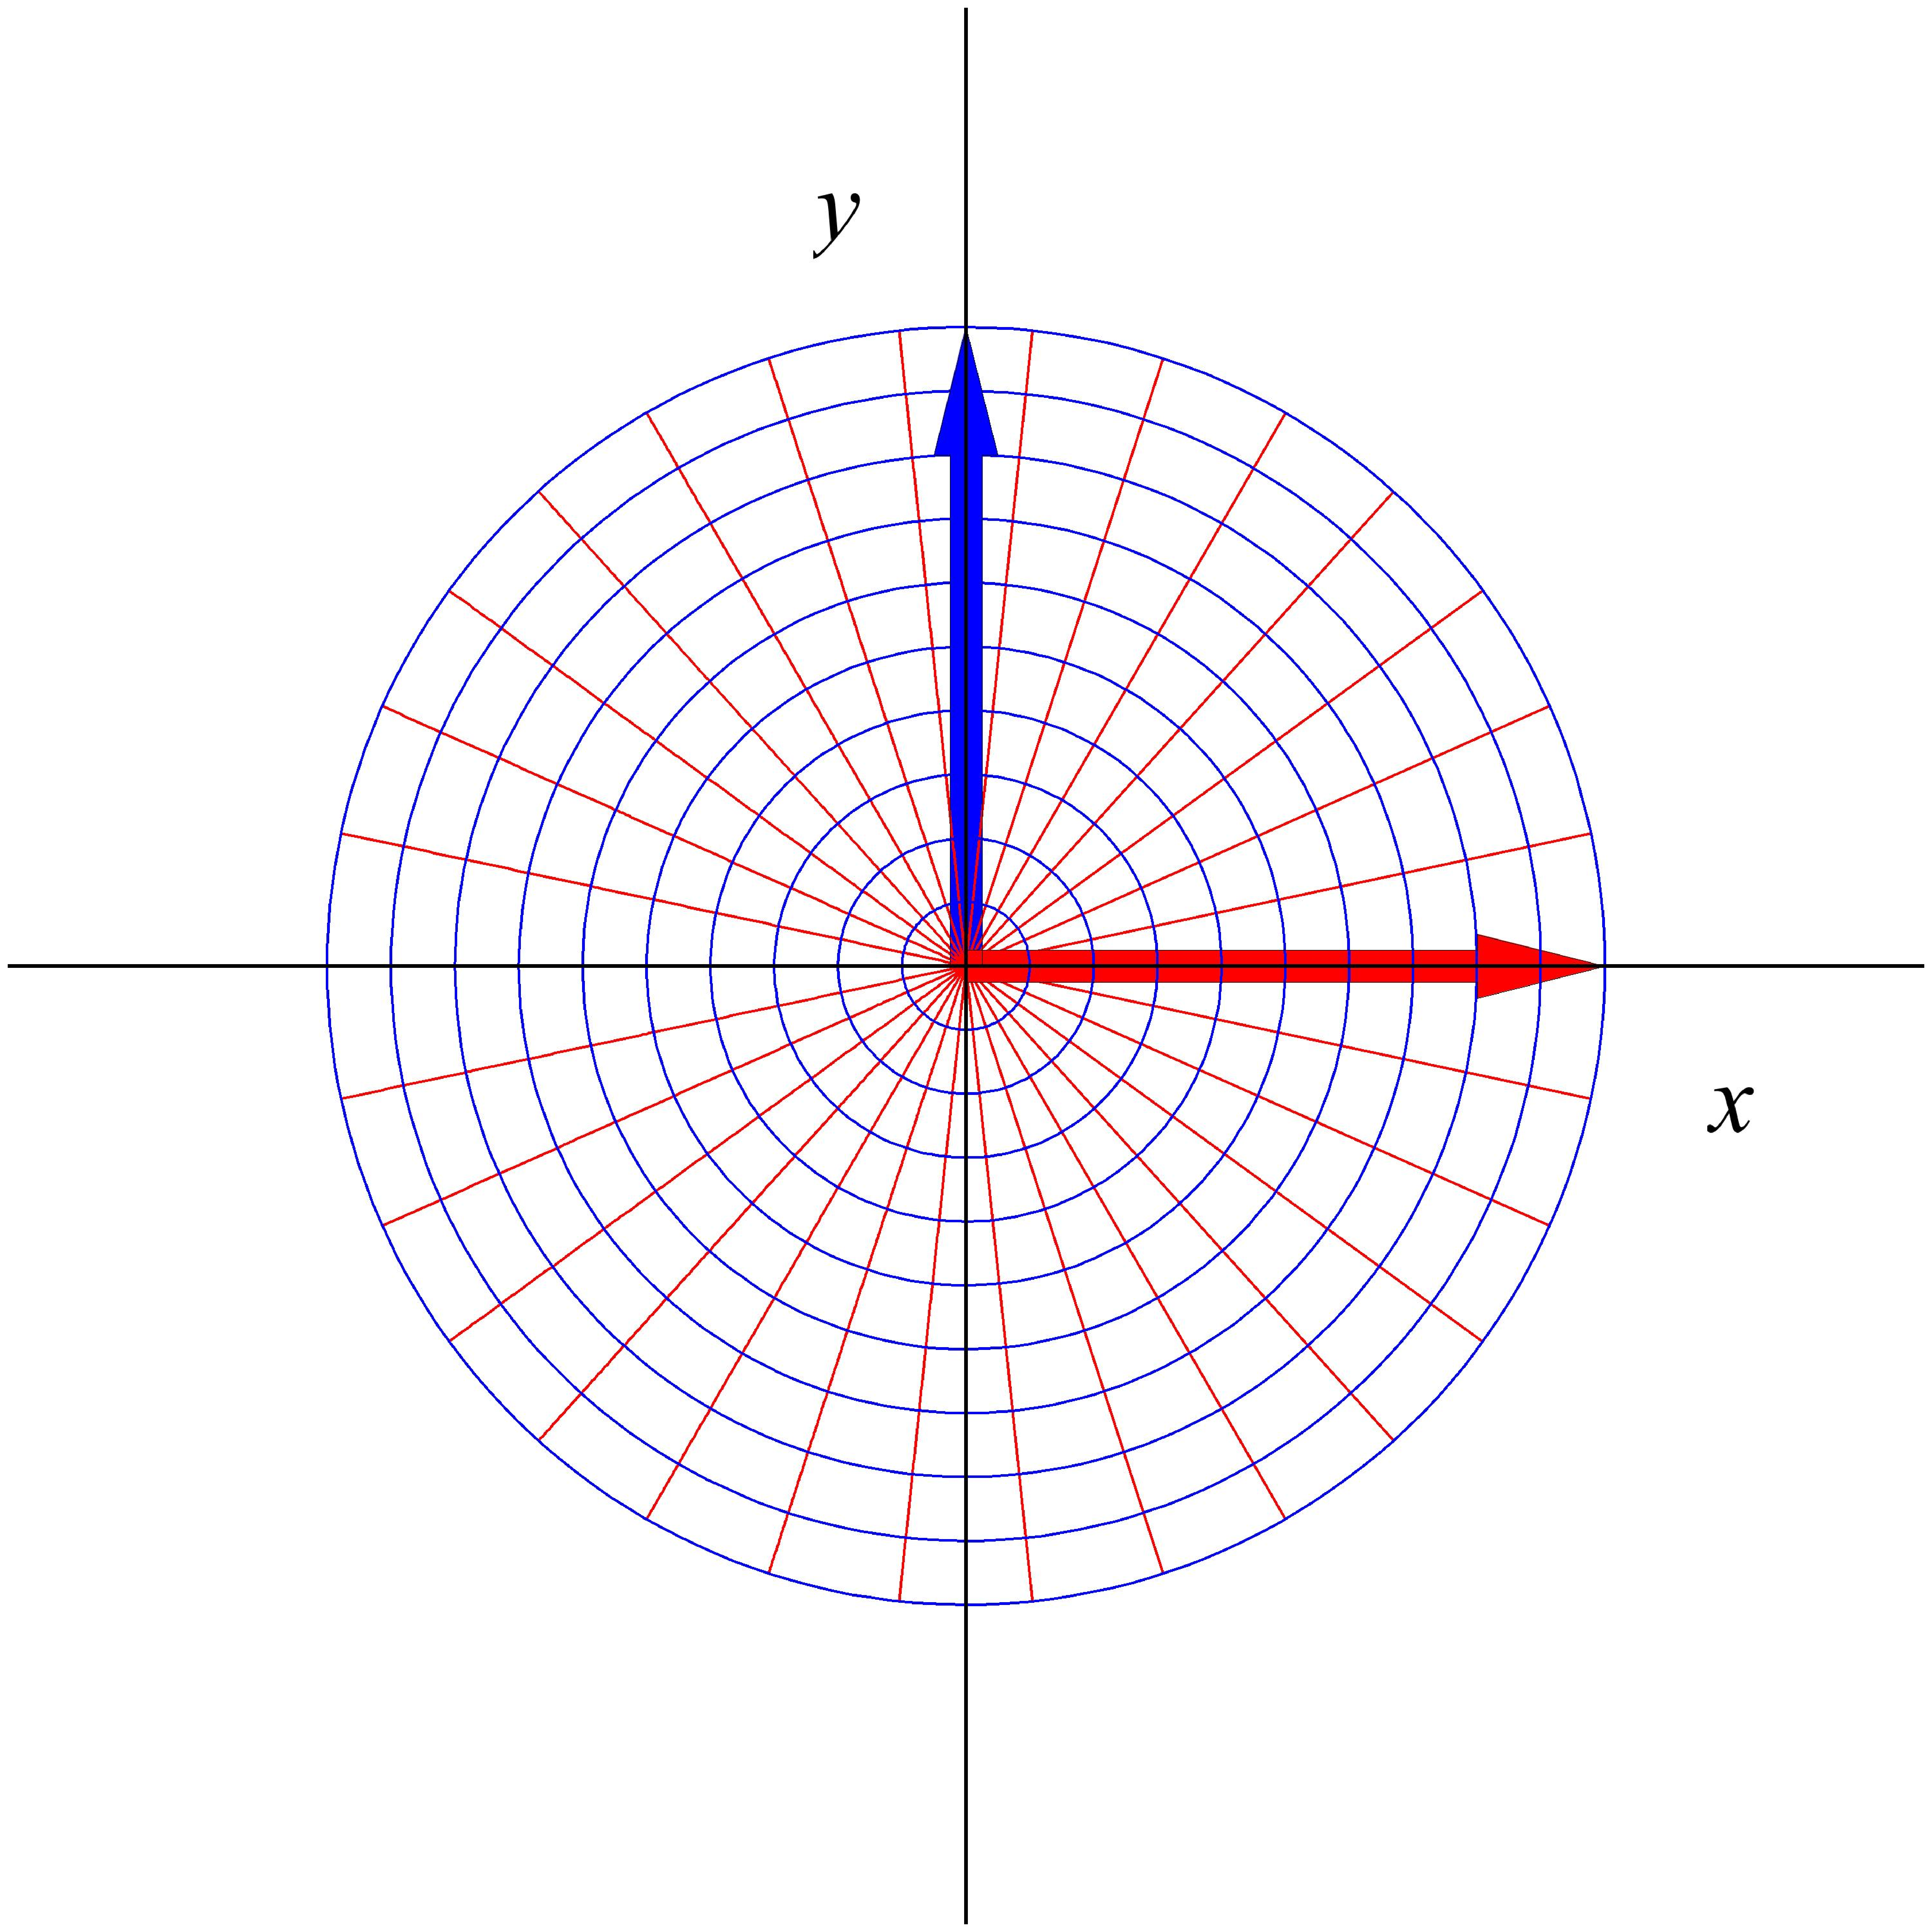
\includegraphics[height=40mm]{FIGS/plotPolarApp2}\,\,\,\,\qquad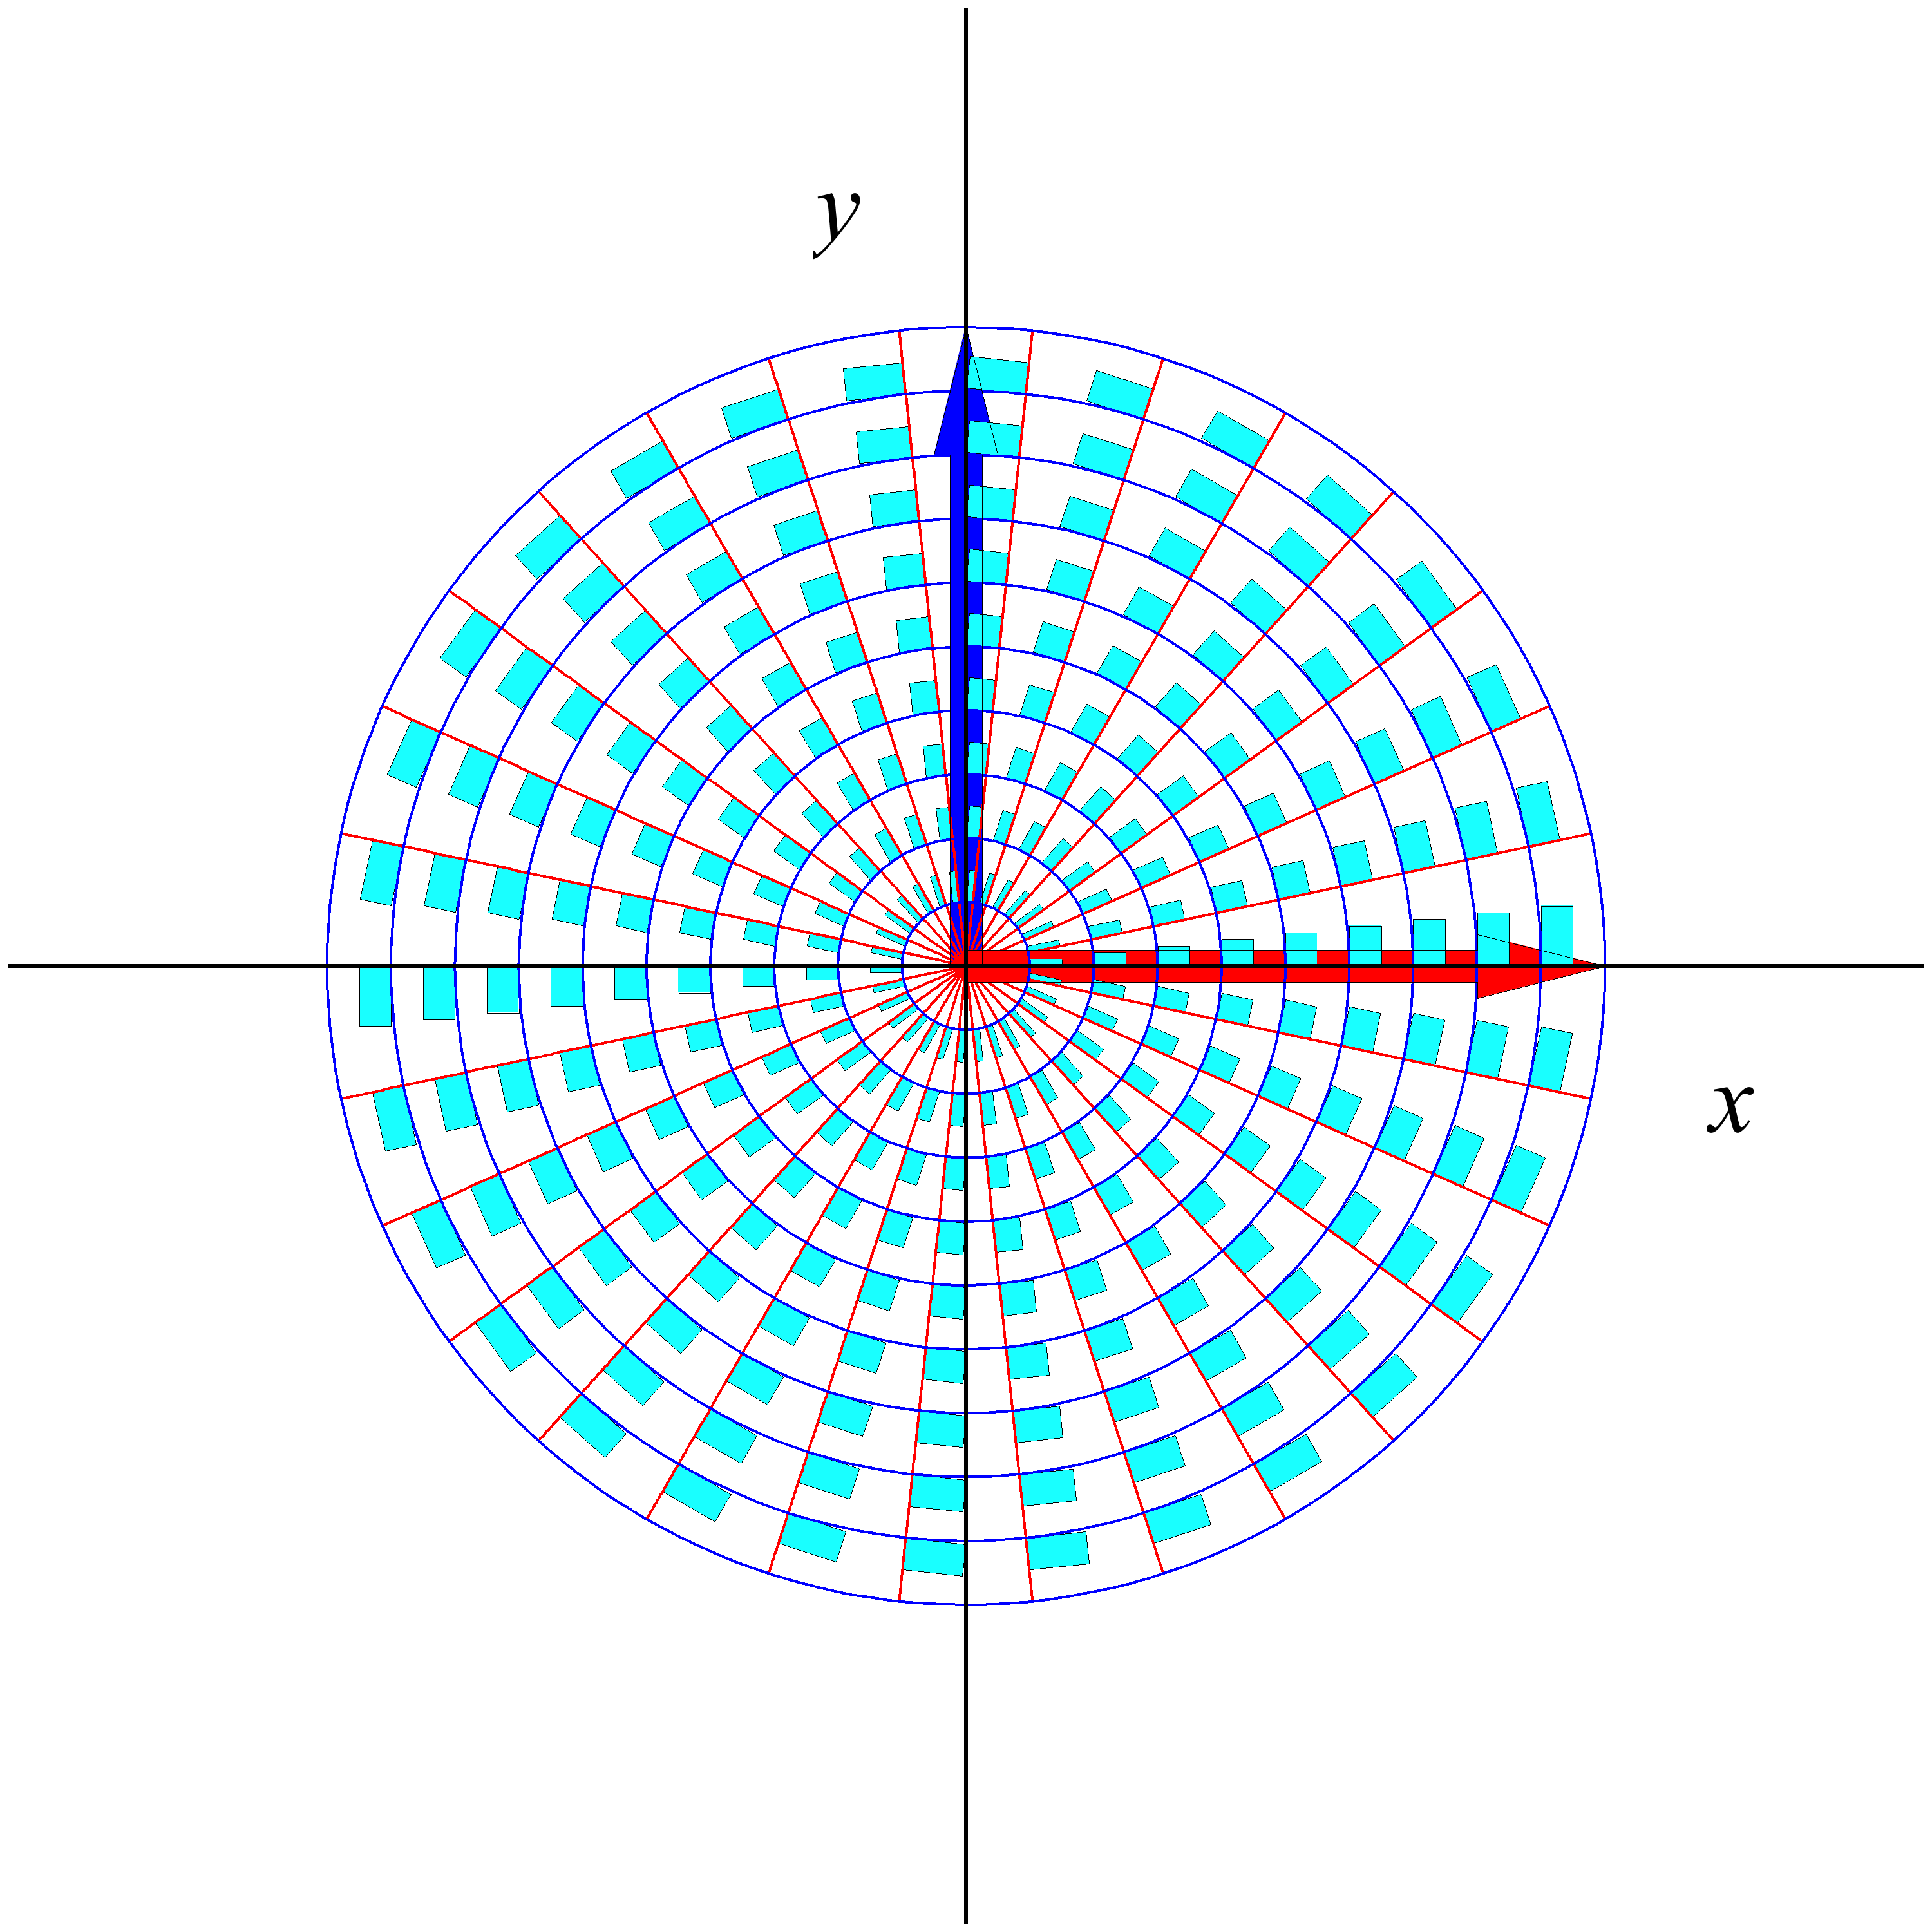
\includegraphics[height=40mm]{FIGS/plotPolarApp3}}
\begin{center}
\caption{\small{Dette område i planen  er givet
ved følgende parameterfremstilling, der
repræsenterer {\em{{polære koordinater}}} i planen:
${\bf r}(u, v) \, = \, (u\cos(v), \, u\sin(v) )
\,\,, \,\, u \in [0, 1 ]\,\, , \, \, v \in [-\pi,
\pi]\,$.
Parameterrektanglet ses til venstre. Den
deformeres og afbildes (ved brug af {\bf{r}}) på
det plane område i midten. Til højre er antydet
placeringen og størrelsen (pånær en faktor $4$)
af de til det givne net hørende approksimerende
parallelogrammer (her er der tale om rektangler).}}
\label{figPolar123}
\end{center}
\end{figure}



Et parametriseret {område i planen} er givet ved en
parameterfremstilling
\begin{equation}
\label{eqPr}
P_{\bf r}: \quad {\bf r}(u,v) \, = \, \left(x(u,v), y(u,v)\right) \in \mathbb{R}^2 \quad , \, \, \,  u \in [a,b] \, \,
, \, \,  v \in [c,d] \quad,
\end{equation}
hvor $x(u,v)$ og $y(u,v)$ er givne (typisk glatte) funktioner af de to parameter-variable $u$ og $v$.\\

Planintegraler opstilles, betegnes, og beregnes helt analogt til kurveintegralerne:


\begin{definition}[Planintegral] \label{defPlanInt}
Lad $f(x,y)$ betegne en kontinuert funktion på $\mathbb{R}^{2}$.
Planintegralet af funktionen $f$ over det parametriserede område
$P_{\bf r}$ defineres ved
\begin{equation} \label{eqPlanIntegral}
\int_{P_{\bf r}} f \, d\mu \, = \, \int_{c}^{d} \int_{a}^{b}
f({\bf r}(u,v))\, \Jac_{\bf r}(u,v)\,du \, dv \quad,
\end{equation}
hvor Jacobi-funktionen $\Jac_{\bf r}(u,v)$,
\begin{equation} \label{eqJacPlan}
 \Jac_{\bf r}(u,v)\, = \,
 | {\bf r}'_{u}(u,v) | \cdot | {\bf
r}'_{v}(u,v) | \cdot \sin(\theta(u,v)) \quad,
\end{equation}
er arealet af det parallelogram {\em{i planen}}, der på
stedet ${\bf r}(u,v)$ udspændes af de to
tangentvektorer ${\bf r}'_{u}(u,v)$ og ${\bf
 r}'_{v}(u,v)$ til de respektive koordinatkurver igennem punktet
${\bf r}(u,v)$ i planen (funktionen $\theta(u, v)\in [0, \pi]$
betegner vinklen mellem disse tangentvektorer).
\end{definition}




\begin{figure}[ht]
\centerline{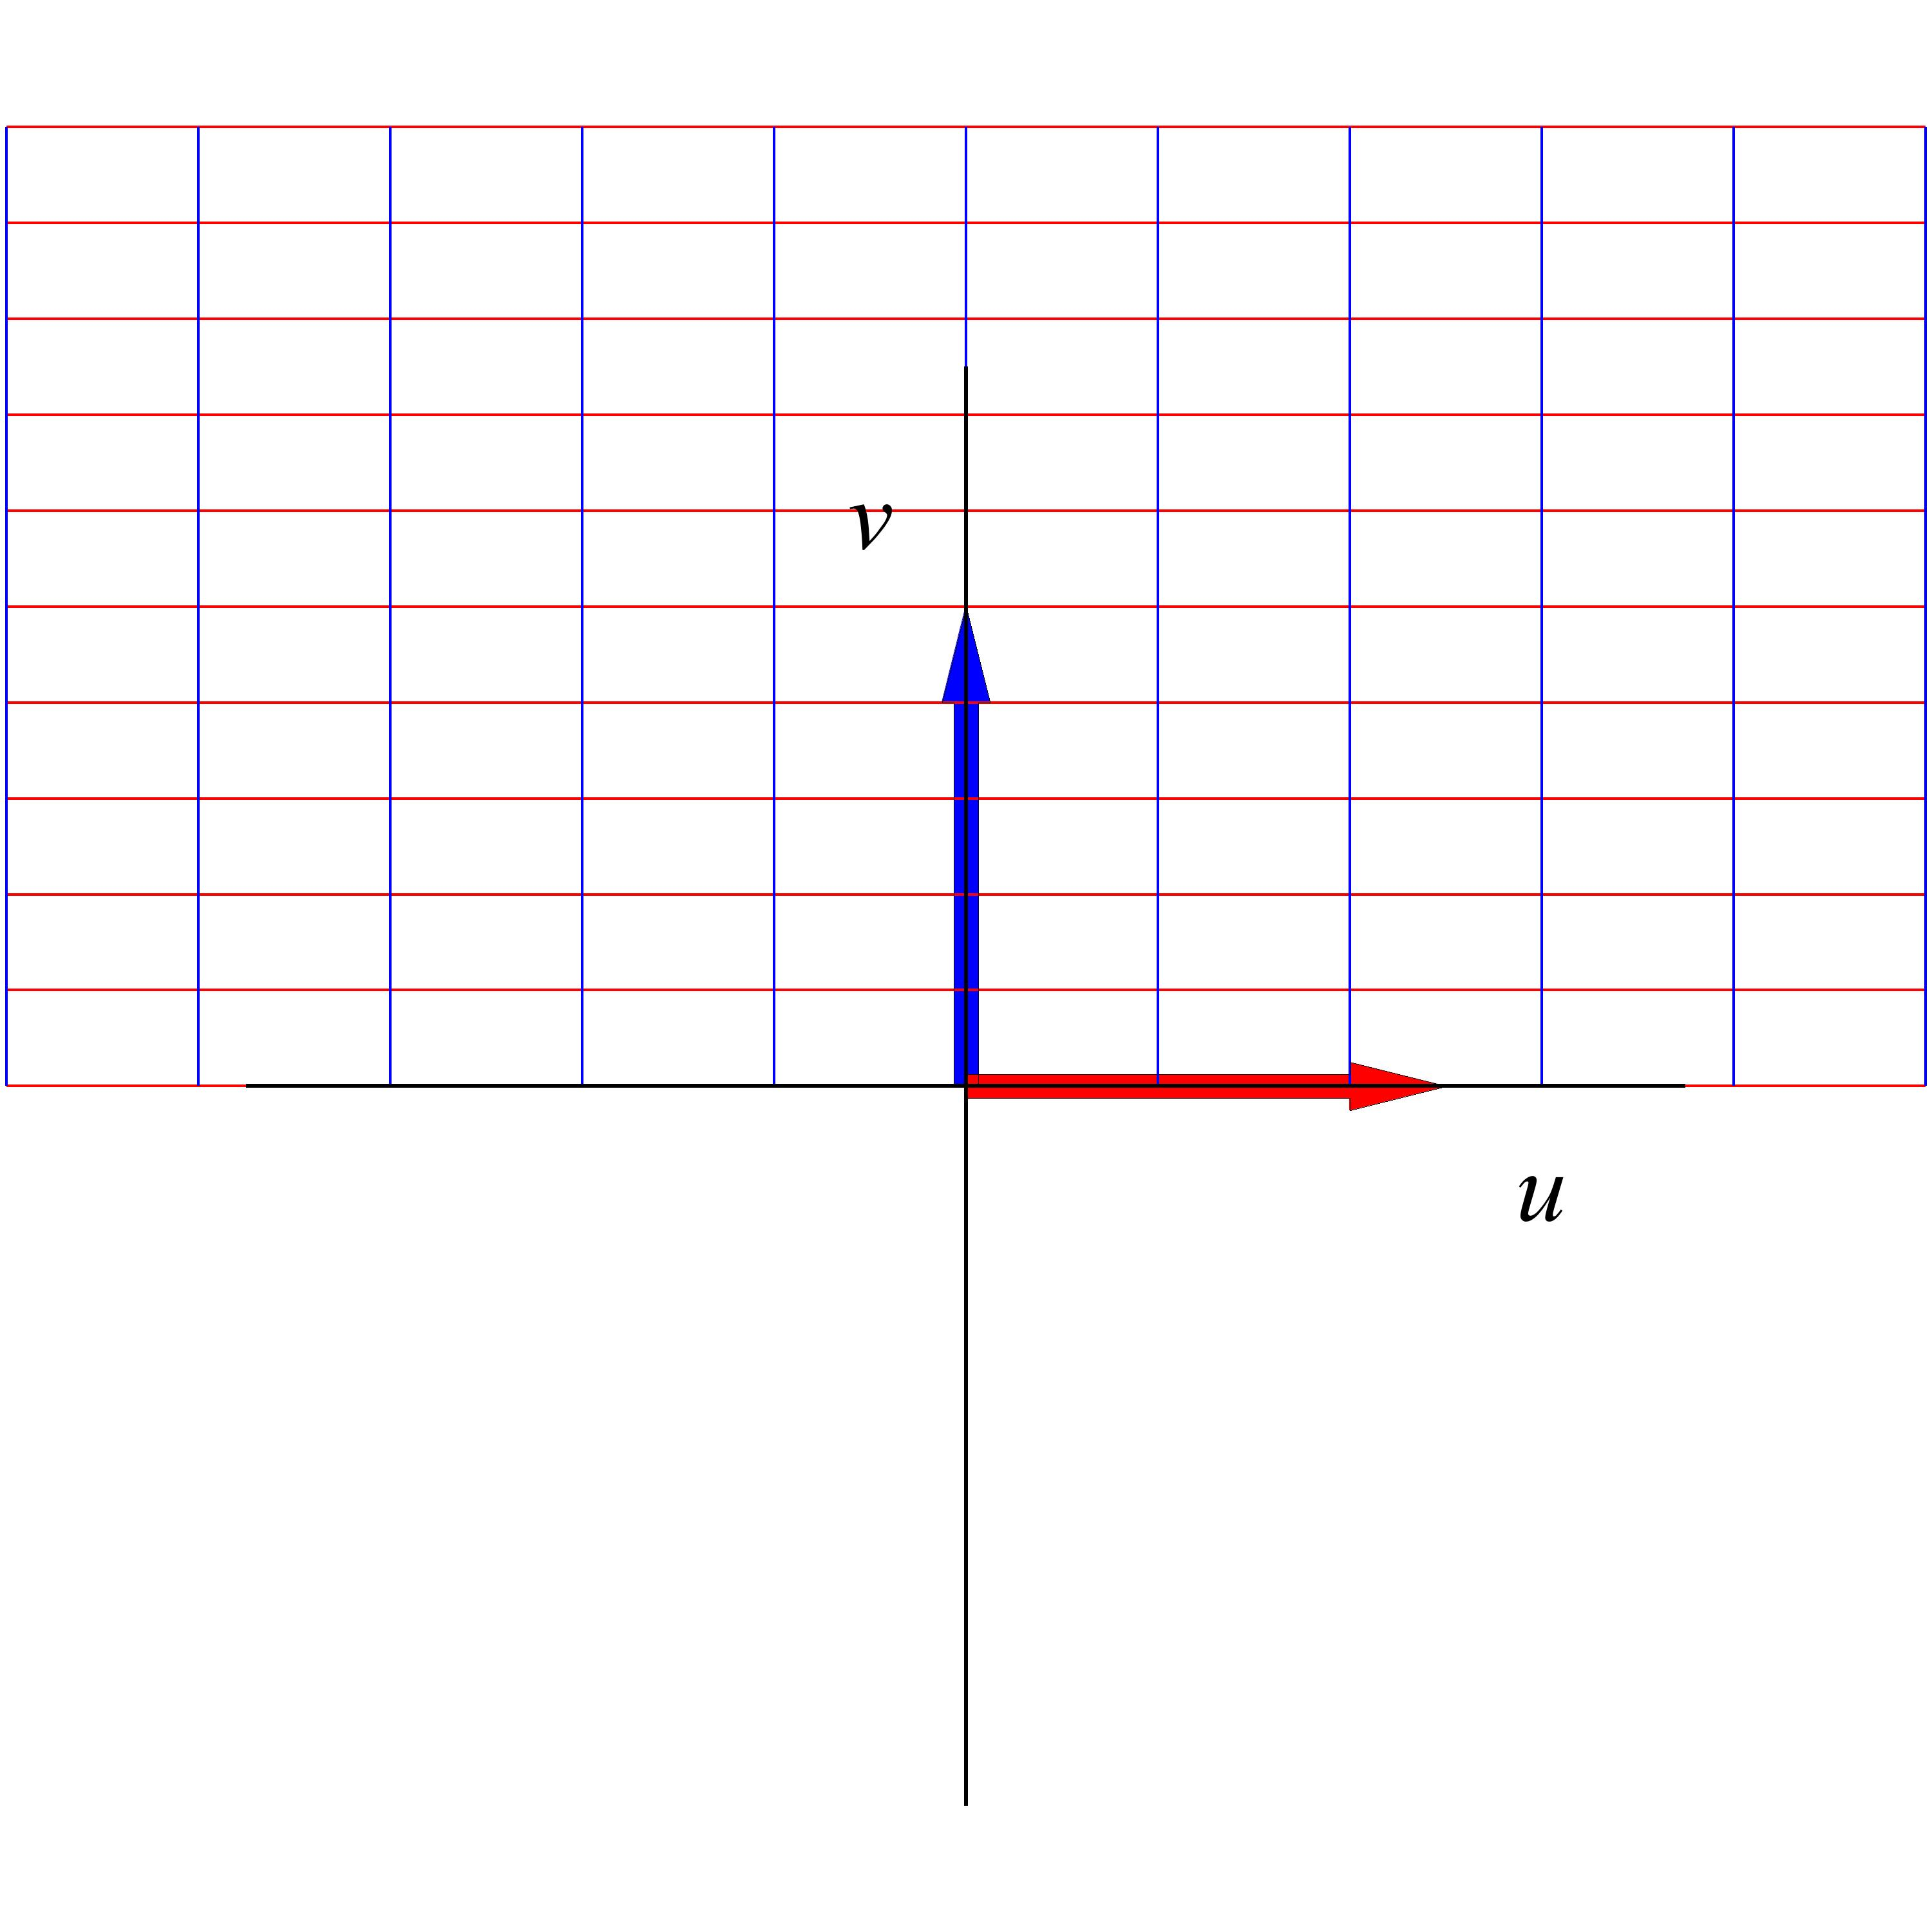
\includegraphics[height=30mm]{FIGS/plot2dParab1} \qquad 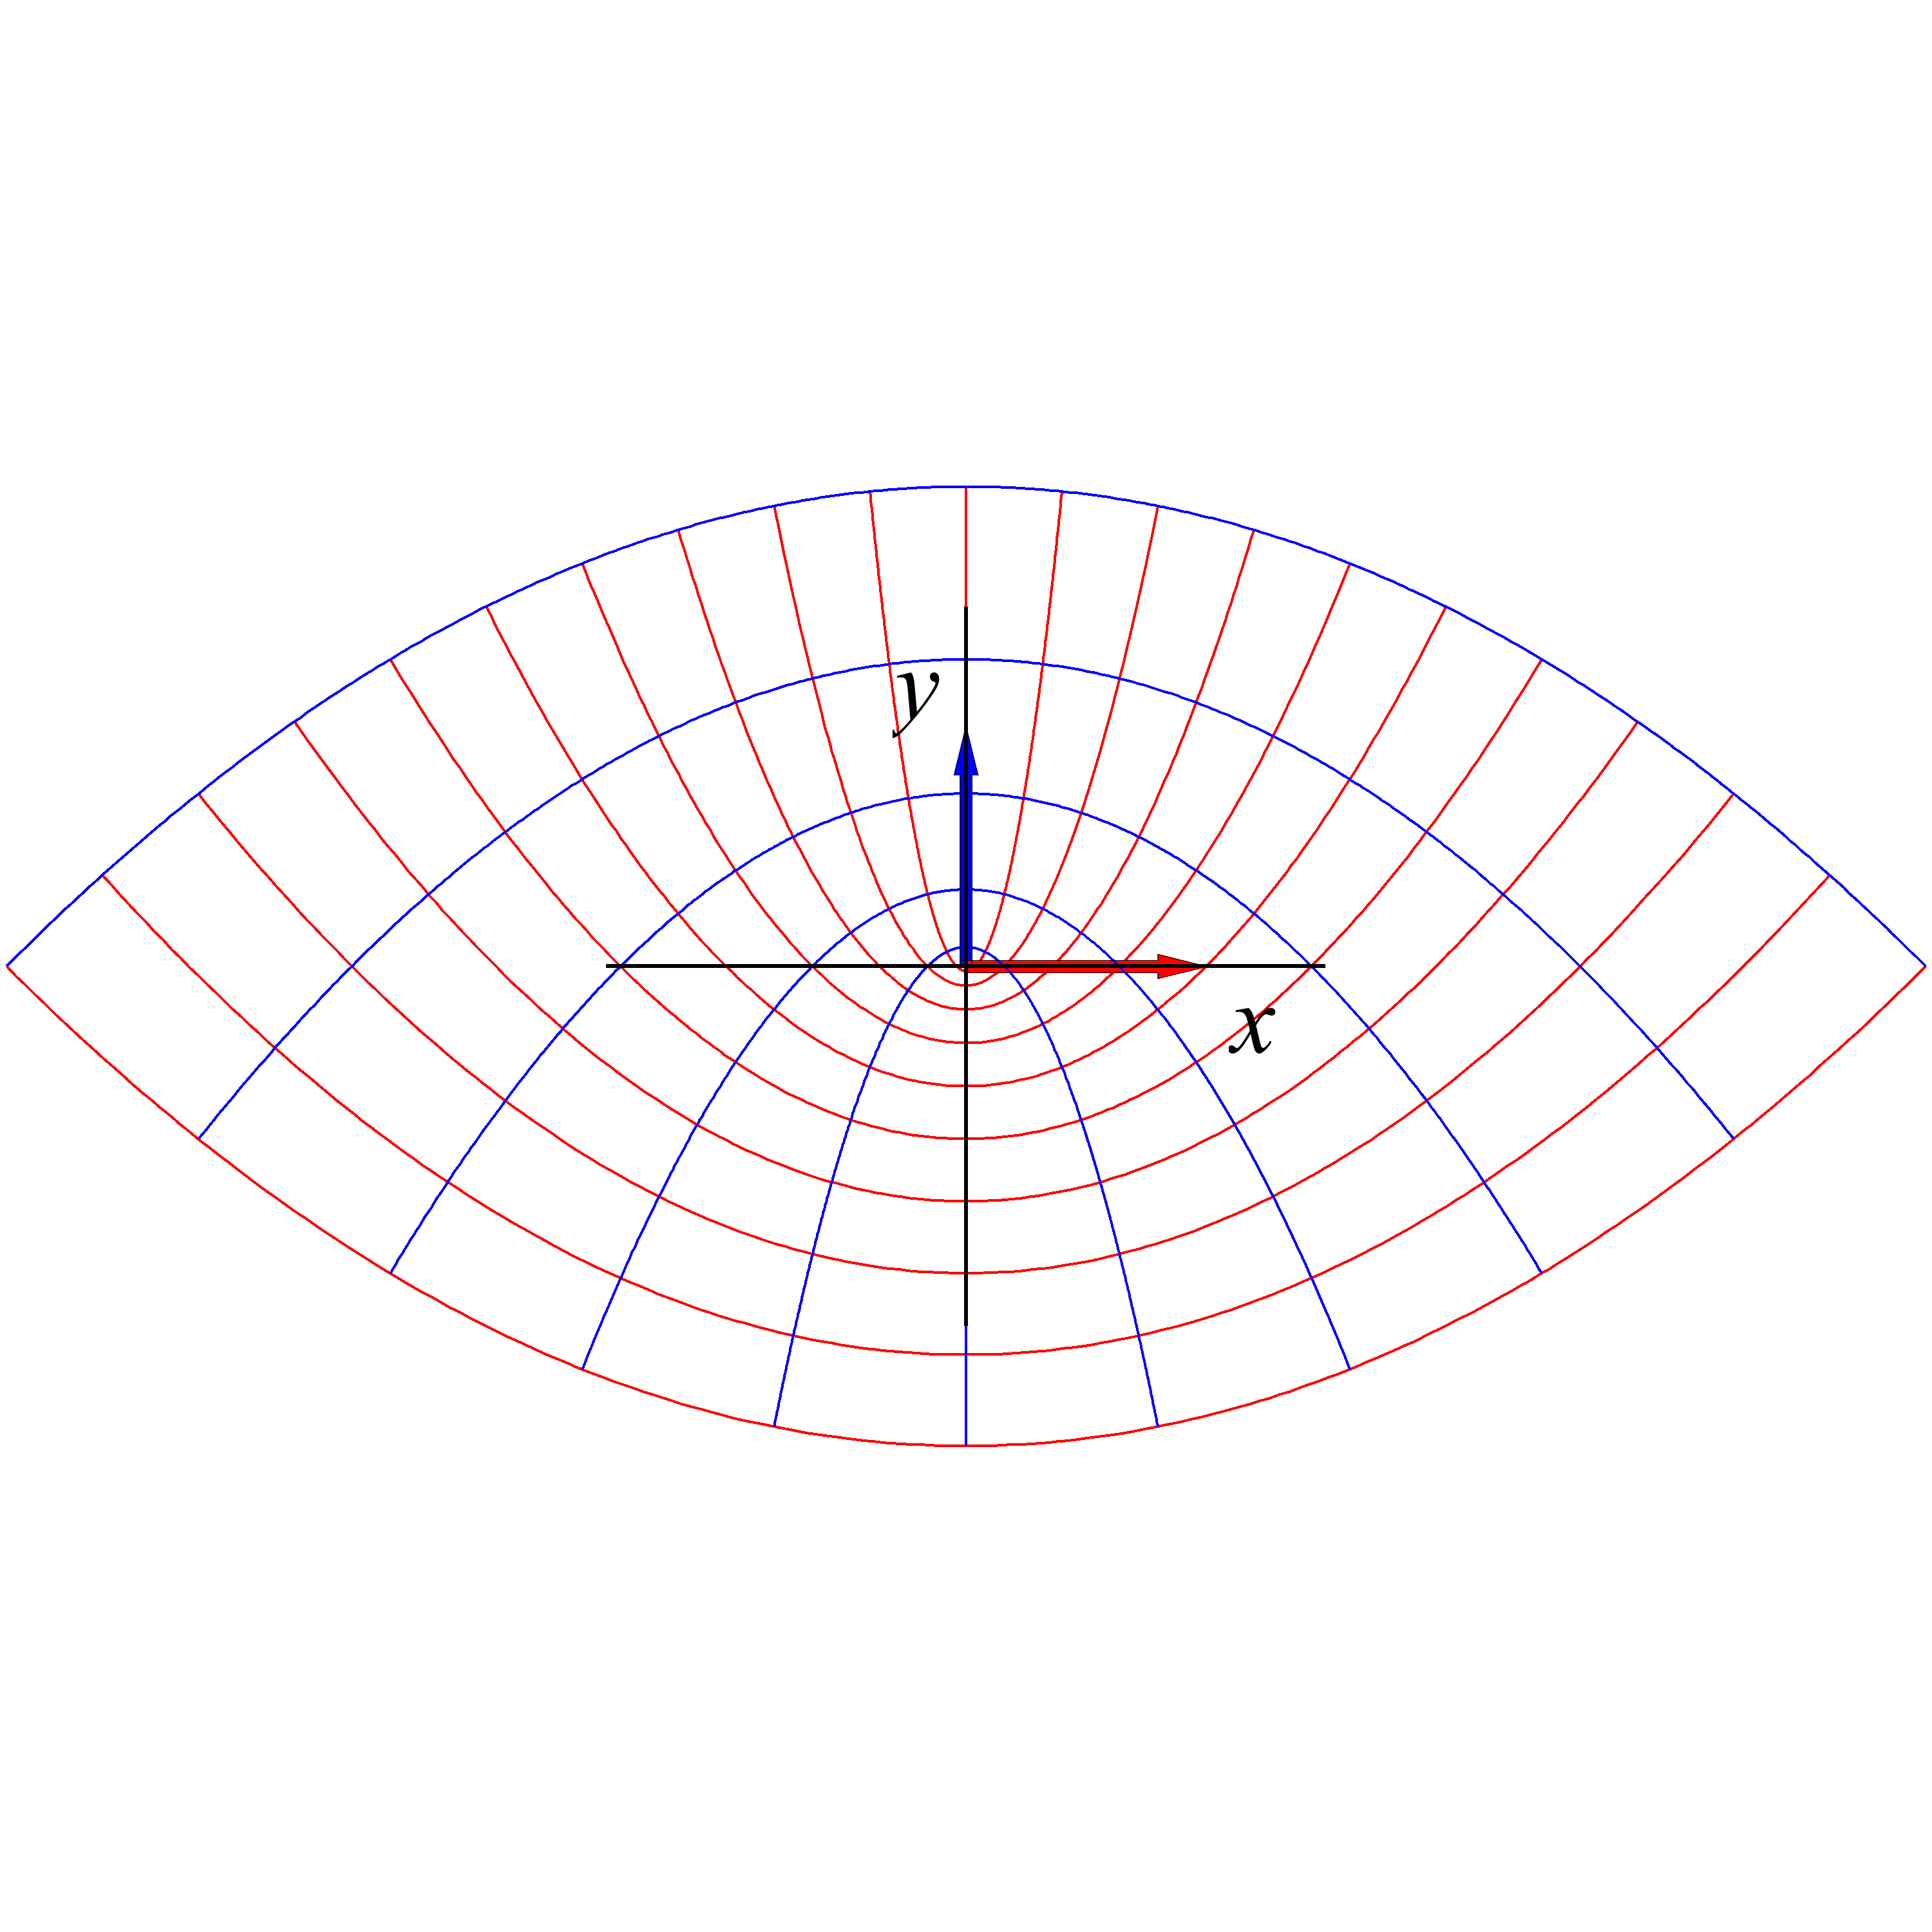
\includegraphics[height=60mm]{FIGS/plot2dParab2} \qquad 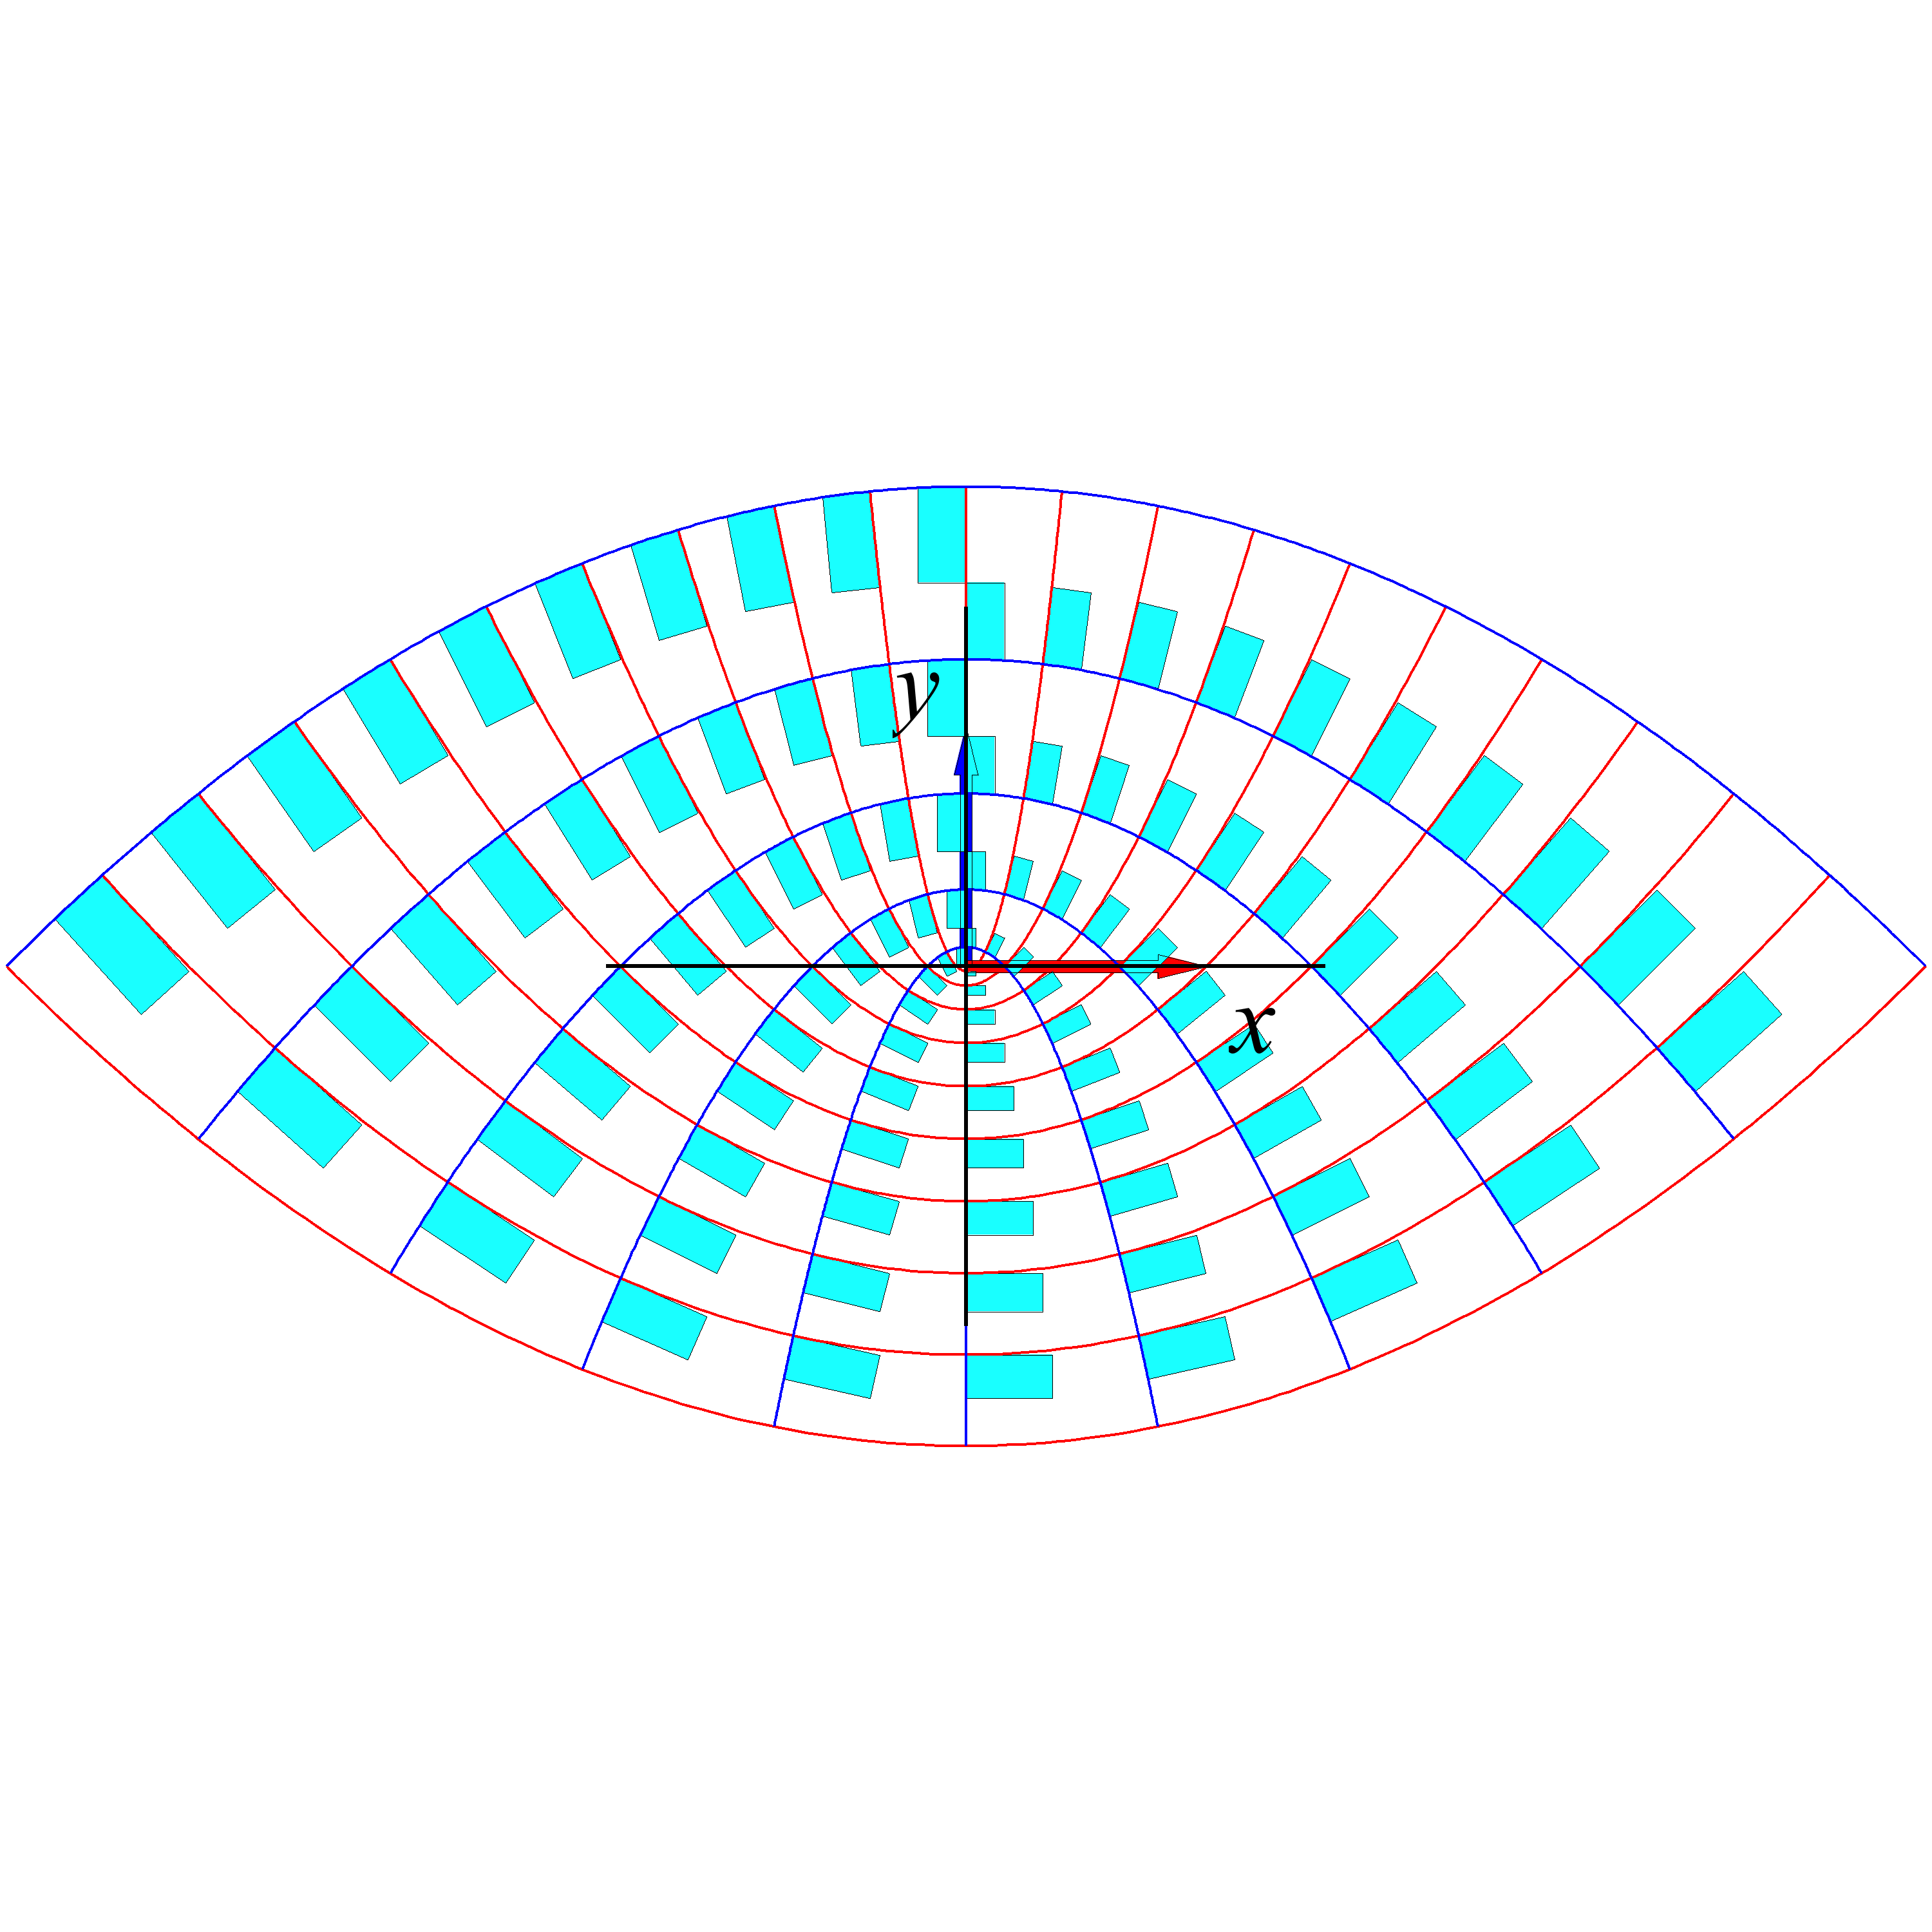
\includegraphics[height=60mm]{FIGS/plot2dParab3} }
\begin{center}
\caption{\small{Plant område med parabelkoordinater. Dette område
i planen  er givet ved para\-me\-ter\-frem\-stillingen
${\bf r}(u, v) \, = \, (u\,v, \frac{1}{2}(u^{2} -
v^{2}) ) \,\,, \,\, u \in [-2, 2 ]\,\, , \, \, v
\in [0,2]\,$. Figuren til højre antyder igen et
system af areal-approksimerende parallelogrammer pånær faktor $4$.}}
\label{fig2dParab12}
\end{center}
\end{figure}

\begin{definition}[Regulær parameterfremstilling for et område i planen] \label{defRegParamPlan}
Parameterfremstillingen (\ref{eqPr}) siges at være en {\em{{regulær parameterfremstilling}}}
for det plane område hvis der gælder følgende:
\begin{equation} \label{eqJacPlanpos}
\Jac_{\bf r}(u,v)\, > 0 \quad \text{for alle} \quad  u \in [a,b] \, \,
, \, \,  v \in [c,d] \quad.
\end{equation}
\end{definition}


\begin{definition}[En-entydig parameterfremstilling] \label{defEnEnParamPlan}
Som for parametriserede kurver siges parameterfremstillingen i
(\ref{eqPr}) at være {en-entydig} hvis forskellige punkter i
definitionsmængden afbildes i forskellige punkter i billedmængden i
planen.
\end{definition}



\begin{exercise} \label{exercJacDet2}
Vis, at $\Jac_{\bf r}(u,v)$ (i (\ref{eqJacPlan})) også kan findes som den numeriske
værdi af determinanten af den $(2 \times 2)$-matrix, der som søjler har
koordinaterne for de to vektorer $\mathbf{r}'_{u}(u,v)$ og  $\mathbf{r}'_{v}(u,v)$.
\end{exercise}

\begin{example}[Standard graf-afgrænset område] \label{exampStandGraf}
Laf $f(x)$ betegne en positiv funktion på et $x$-interval $[a, b]$. Så kan vi parametrisere området imellem
$x$-aksen og grafen for funktionen $f(x)$ på følgende simple måde:
\begin{equation}
P_{\mathbf{r}} \quad : \quad \mathbf{r}(u,v) = (u, v \cdot f(u)) \quad , \quad  u\in [a, b] \quad , \quad v \in [0, 1] \quad.
\end{equation}
Se figur \ref{figStandGraf} (hvor funktionen $f(x) = 1 + x + x^{2}$ er benyttet til illustration).
Til bestemmelse af arealet af området imellem grafen for $f(x)$ og $x$-aksen har vi nu helt generelt:
\begin{equation}
\Jac_{\mathbf{r}}(u,v) = f(u) \quad ,
\end{equation}
fordi
\begin{equation}
\begin{aligned}
\mathbf{r}'_{u}(u,v) &= (1, v\cdot f'(u)) \quad \textrm{og} \\
\mathbf{r}'_{v}(u,v) &= (0, f(u)) \quad ,
\end{aligned}
\end{equation}
sådan at determinanten af den matrix, der har søjlerne $\mathbf{r}'_{u}(u,v)$ og $\mathbf{r}'_{v}(u,v)$, netop i dette tilfælde er funktionen $f(u)$ selv og dermed er også Jacobifunktionen givet ved $f(u)$ ifølge opgave \ref{exercJacDet2}. Heraf fås det ønskede areal rekonstrueret  som:

\begin{equation}\label{eqIntegratKurve}
\begin{aligned}
\Ar(P_{\mathbf{r}}) = \int_{P_{\mathbf{r}}}\, 1 \, d\mu &= \int_{0}^{1} \left( \int_{a}^{b} \,f(u) \, du \right) \, dv \\
&= \int_{a}^{b}\,f(u) \, du \quad.
\end{aligned}
\end{equation}
Overvej, hvad der sker med integralet i (\ref{eqIntegratKurve}), hvis $f(x)$ tillades at være negativ på givne delintervaller af $[a, b]$.
\end{example}




\begin{figure}[ht]
\centerline{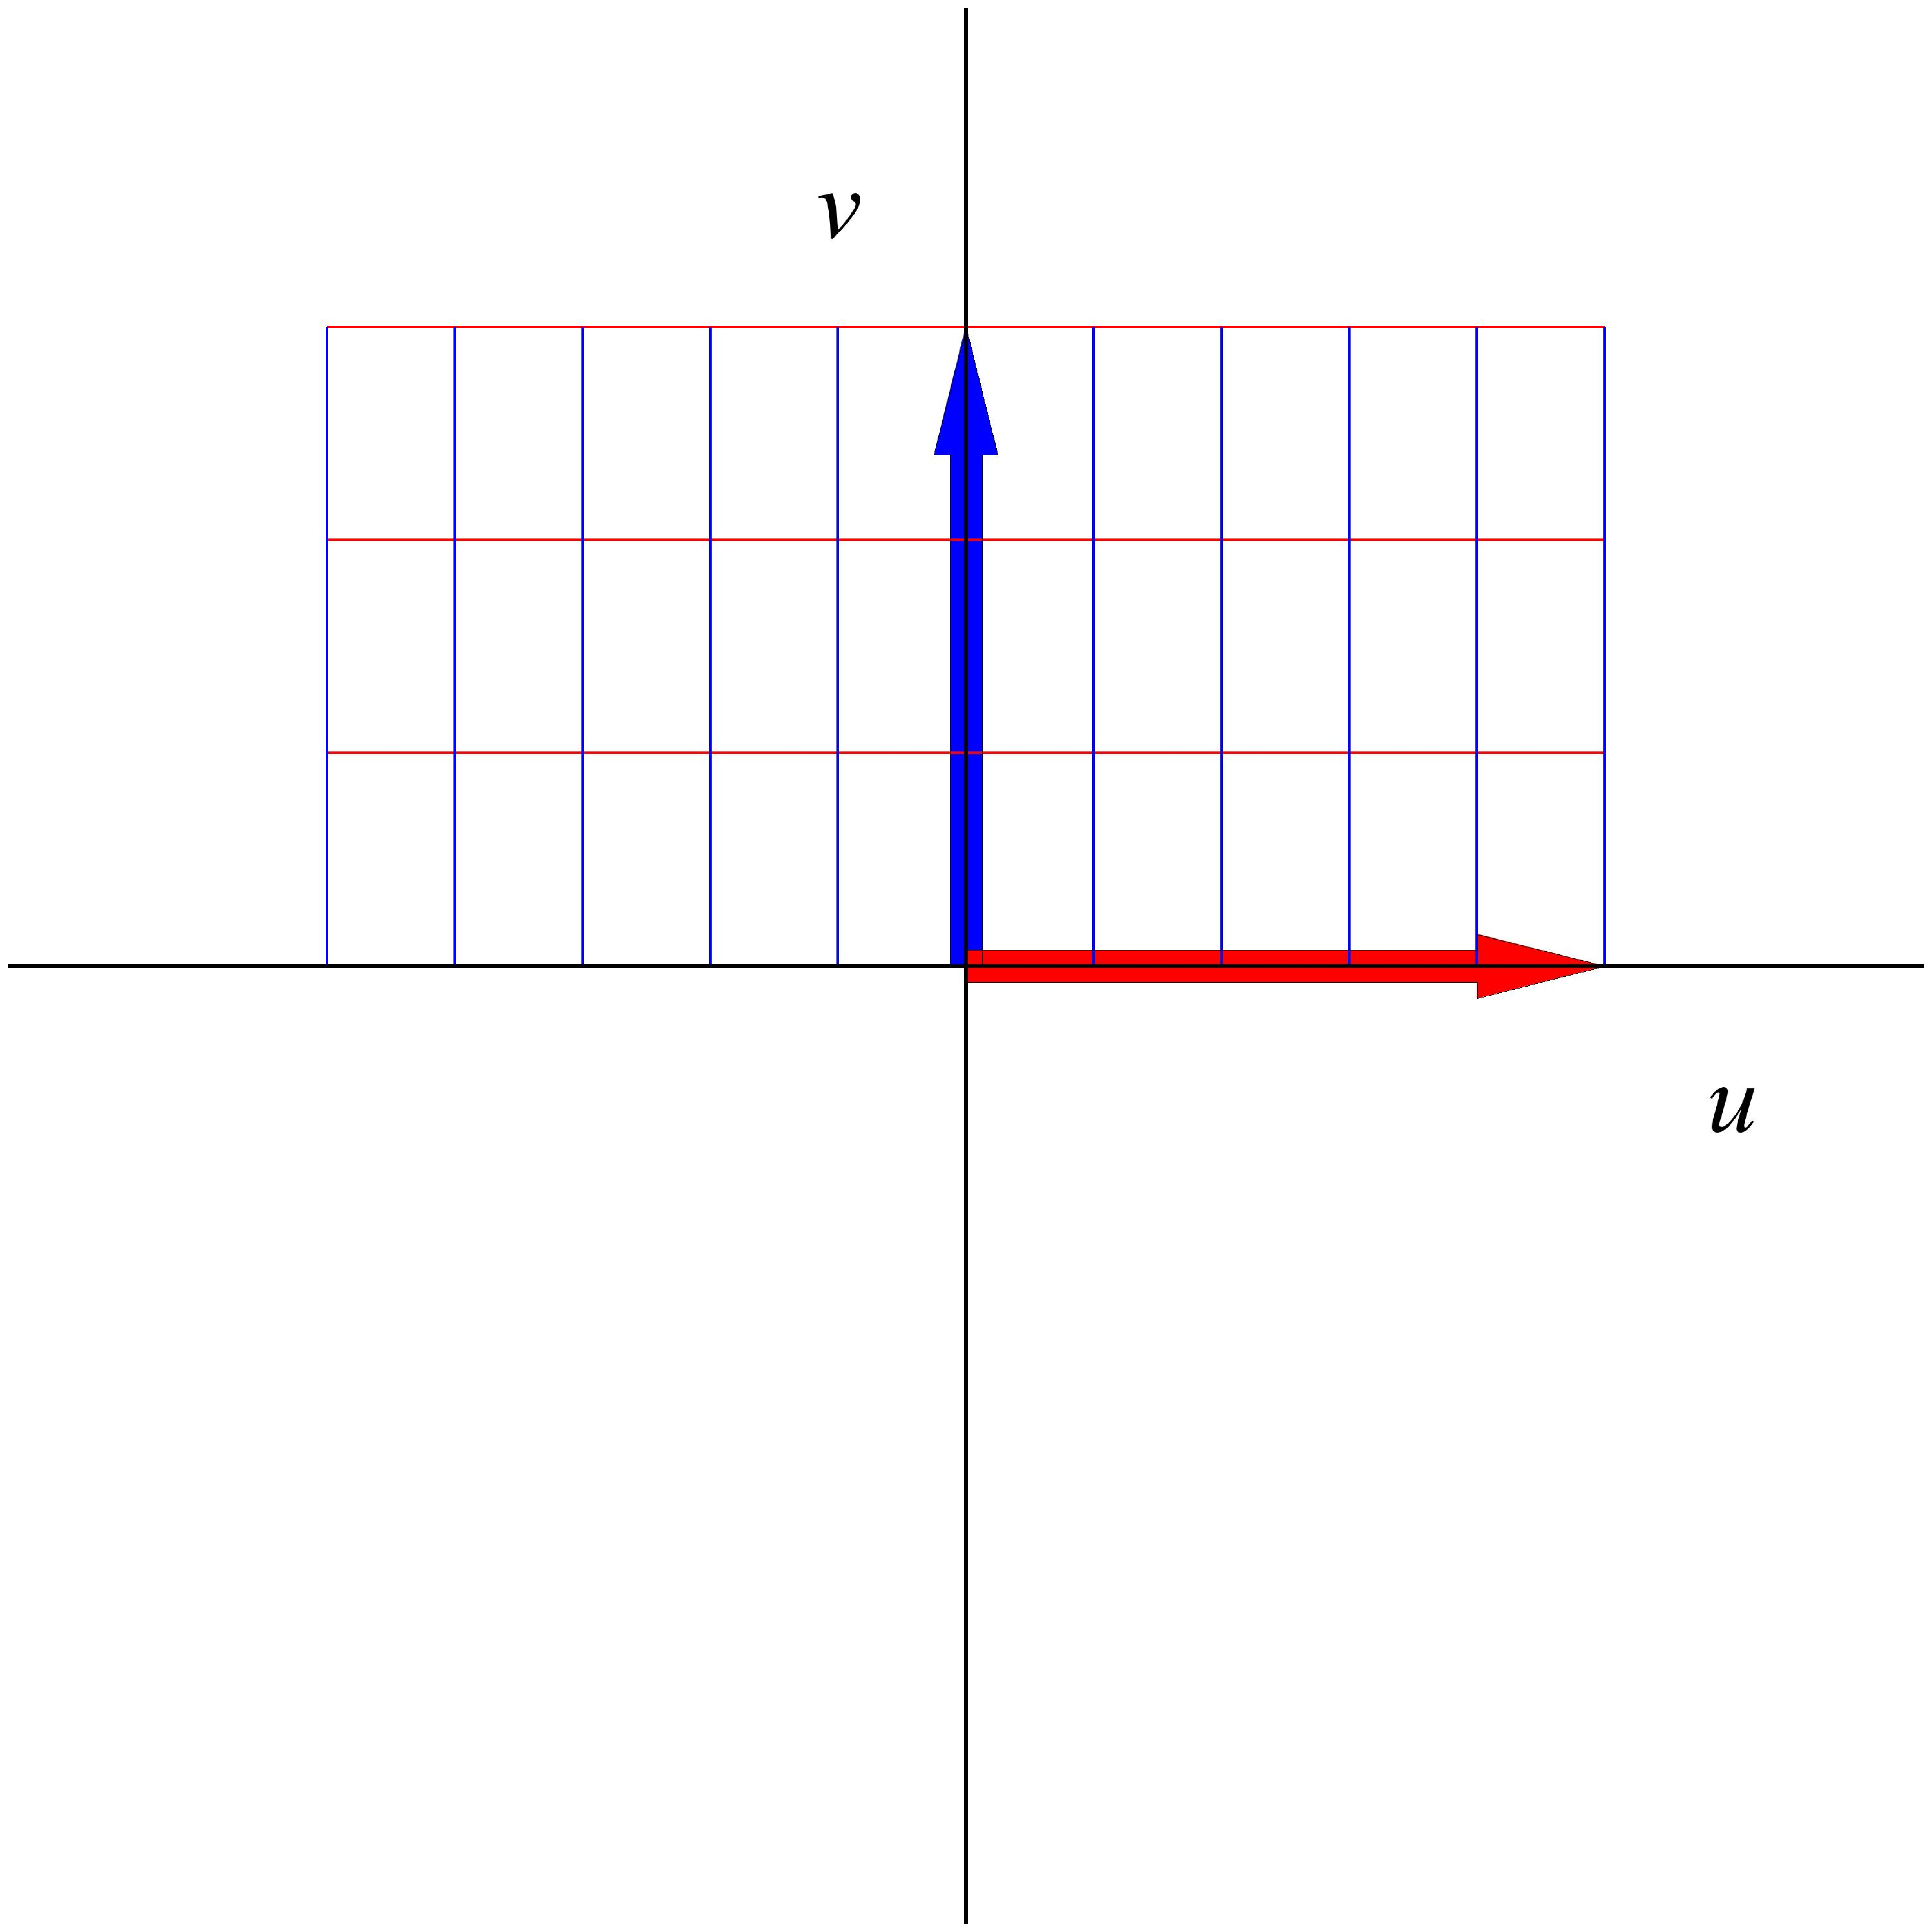
\includegraphics[height=55mm]{FIGS/plotStandGraf1}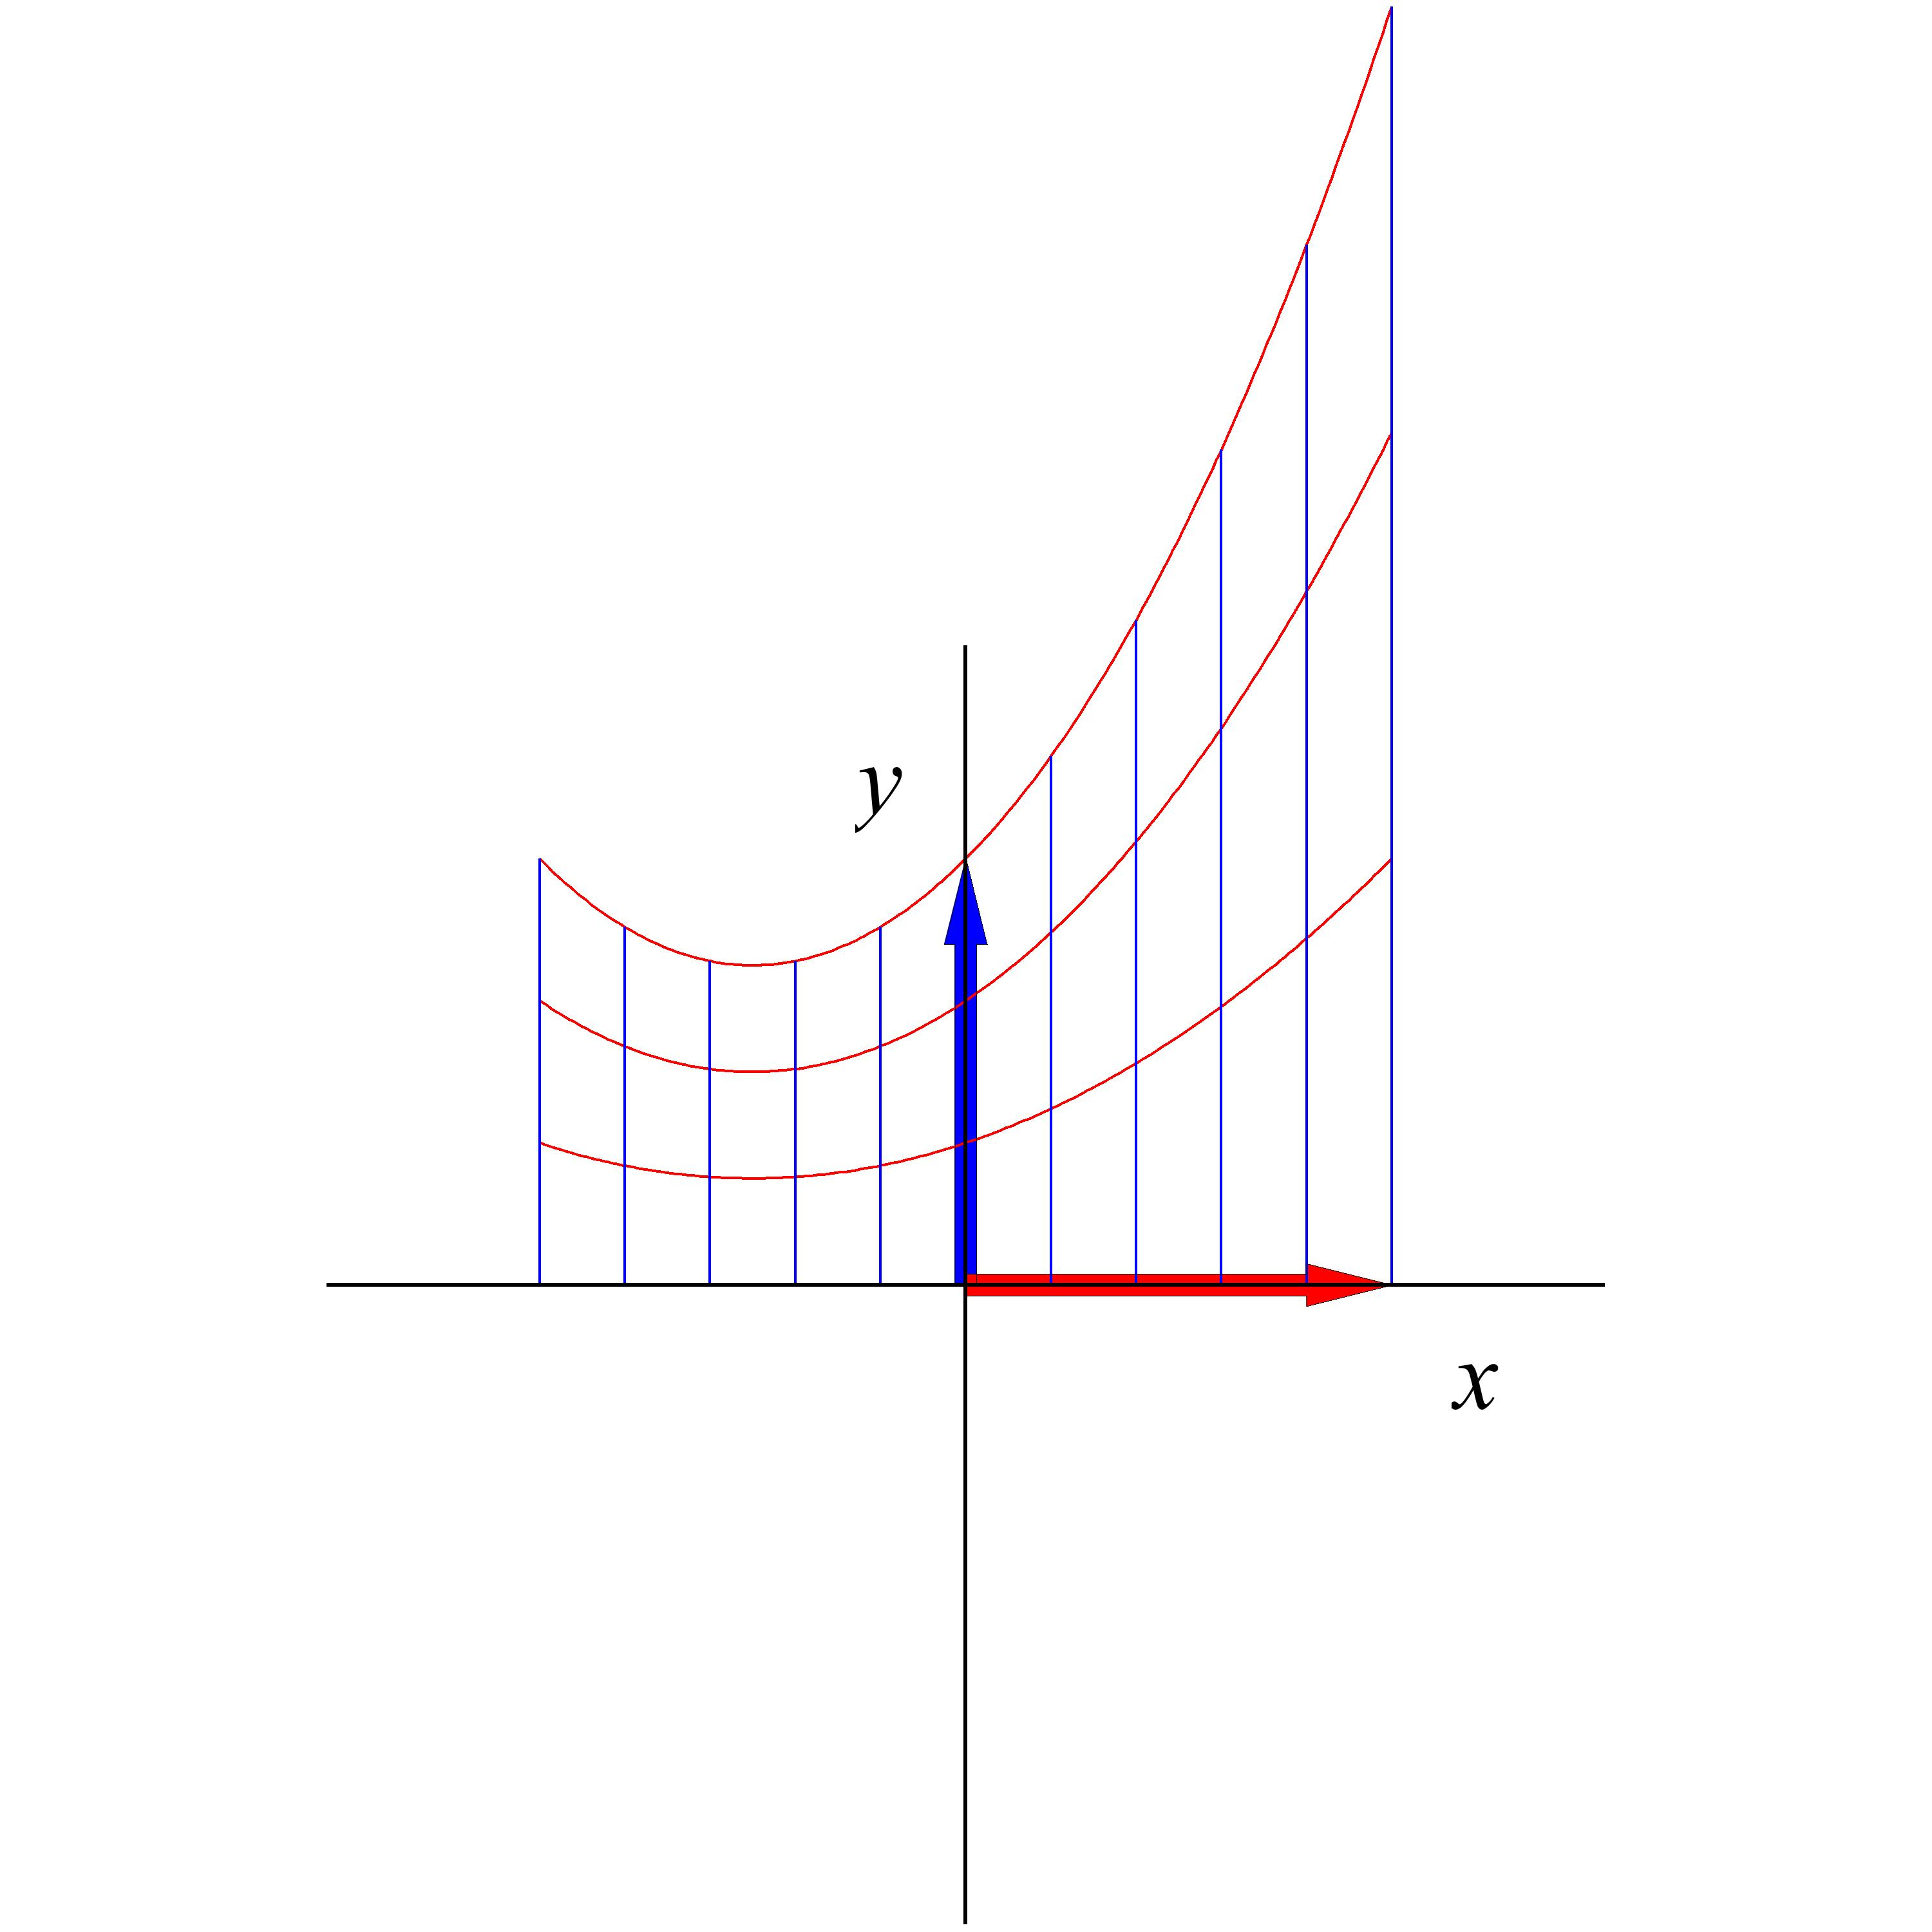
\includegraphics[height=55mm]{FIGS/plotStandGraf2}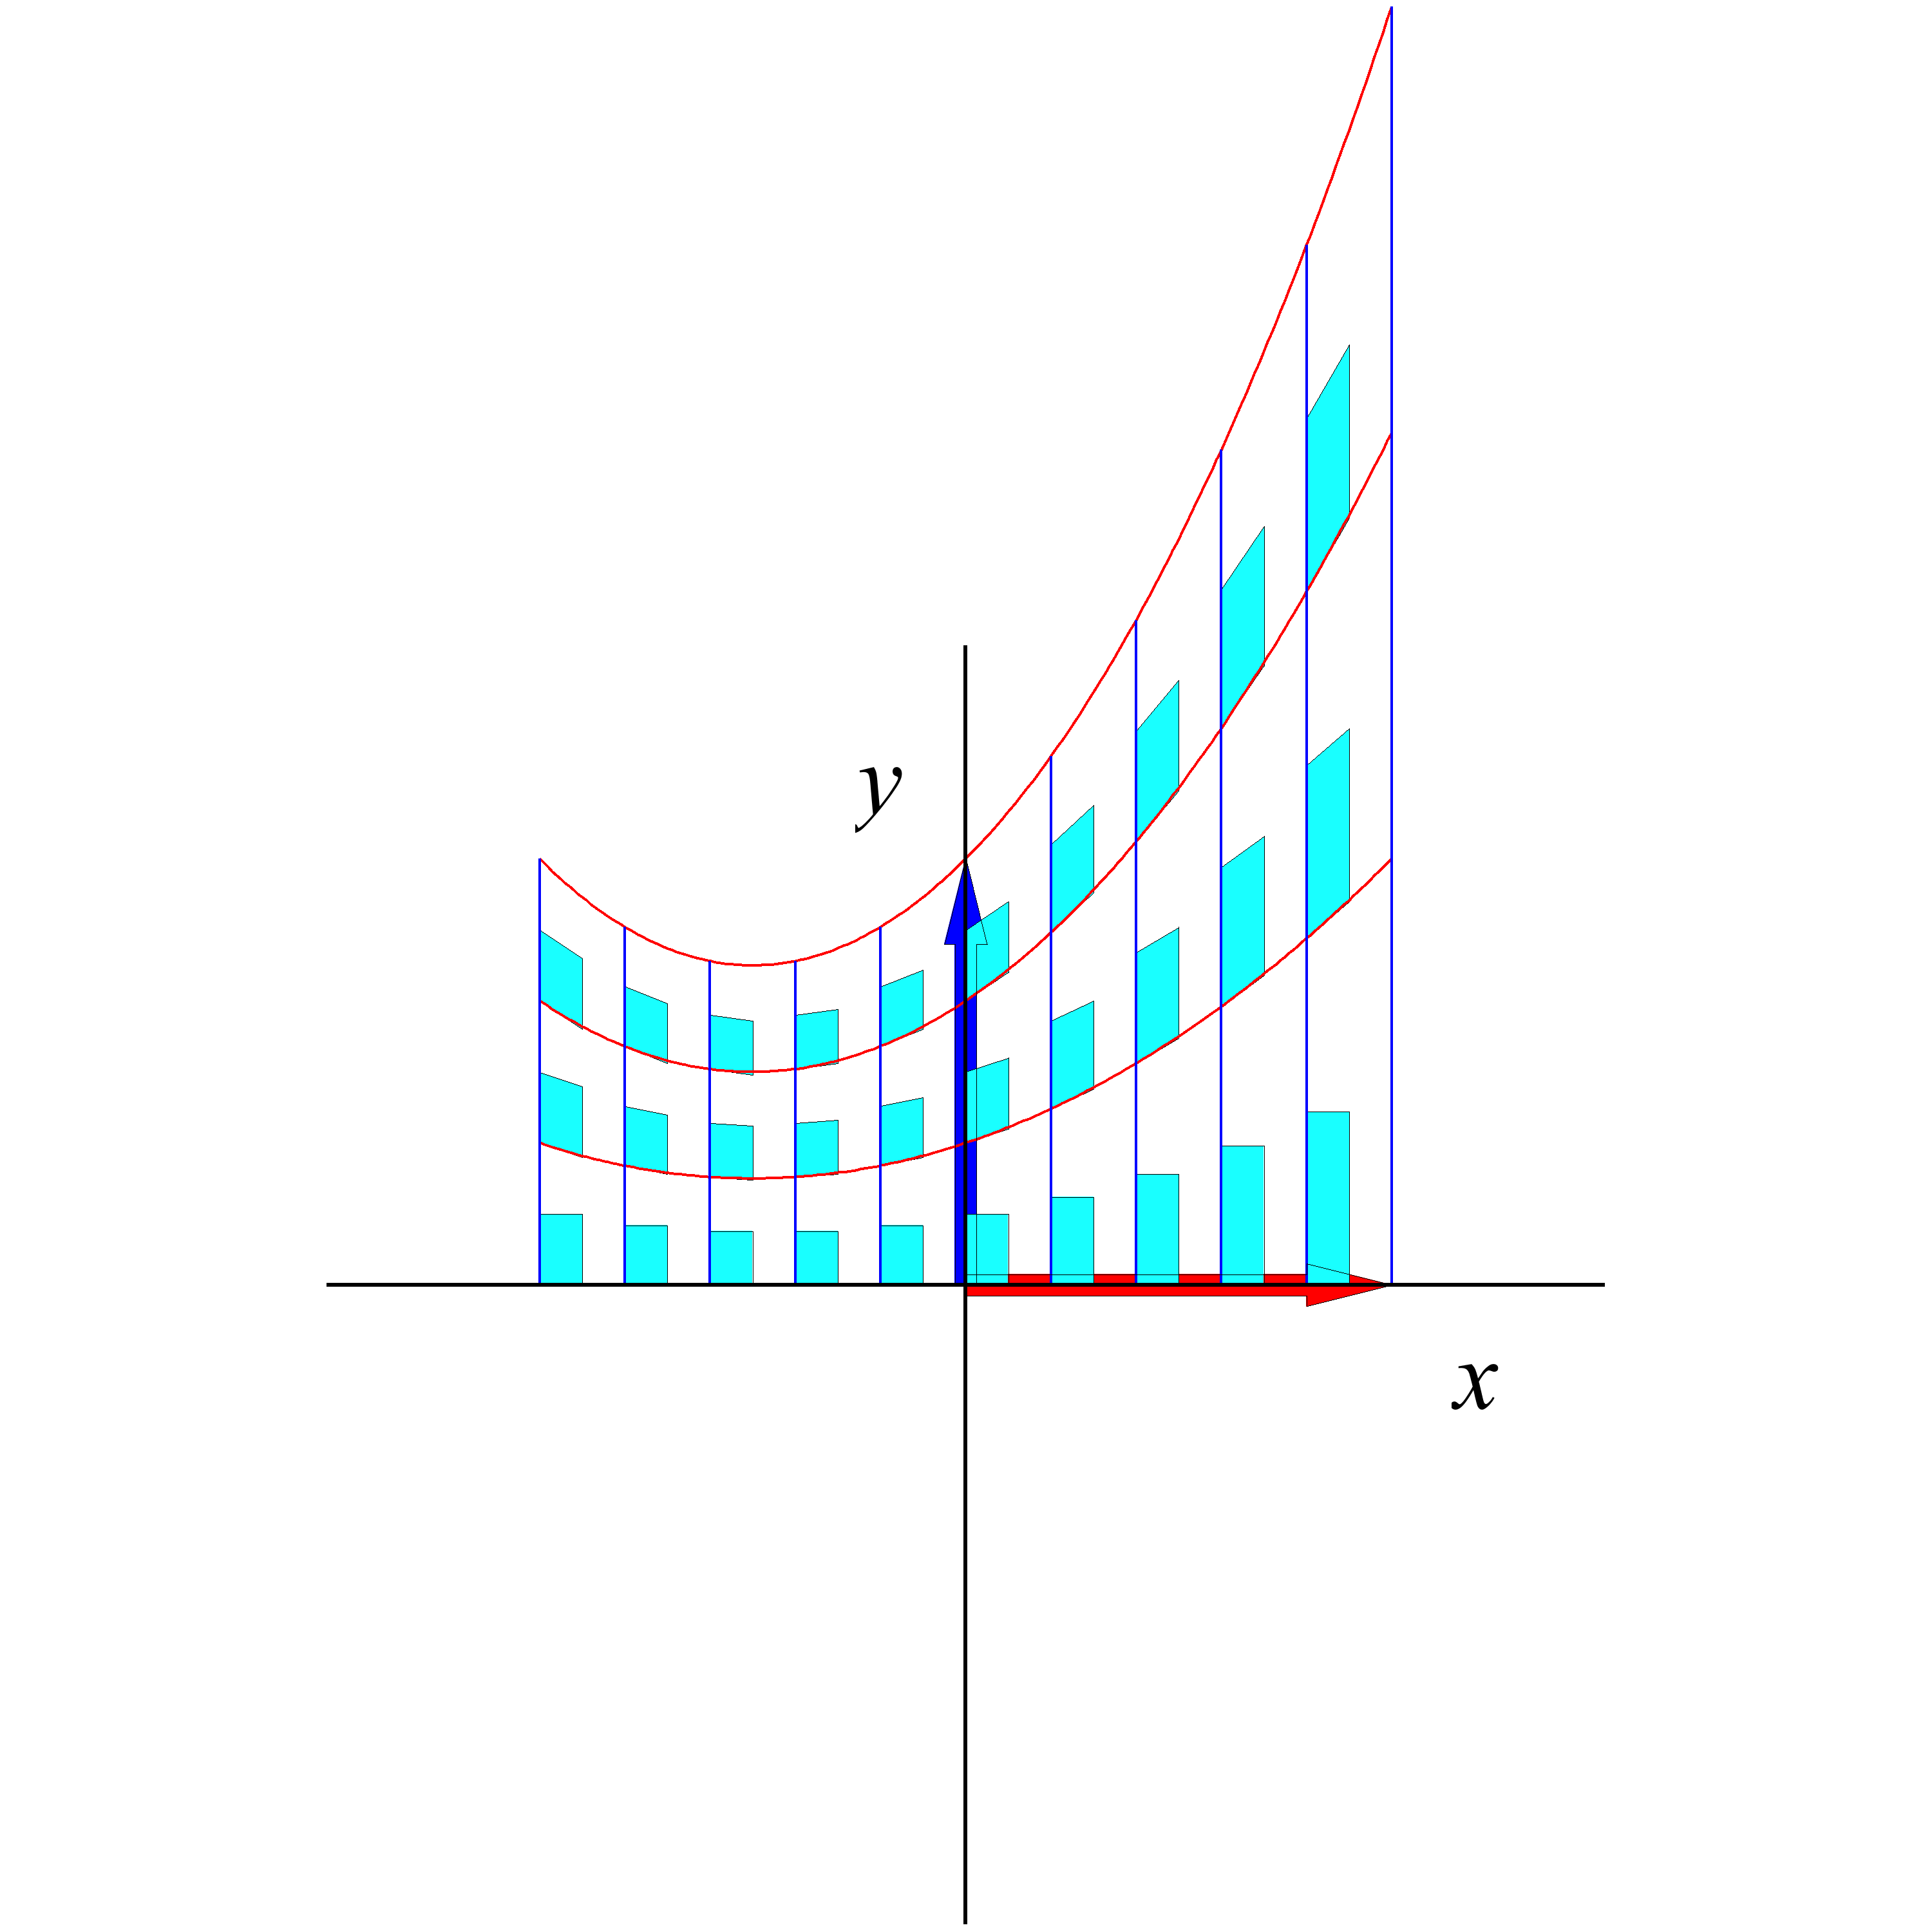
\includegraphics[height=55mm]{FIGS/plotStandGraf3} }
\begin{center}
\caption{\small{Parametrisering af området imellem $x$-aksen og grafen for funktionen $f(x) = 1 + x + x^{2}$. Se
eksempel \ref{exampStandGraf}.}} \label{figStandGraf}
\end{center}
\end{figure}







\begin{example}[Elliptisk område] \label{exEllipseDisk}
Det parametriserede elliptiske område i planen (se figur \ref{figEllipseDisk})
$$
P_{\bf r}: \,\, {\bf
r}(u, v) \, = \, \left(\, av\cos(u), \,bv\sin(u) \, \right) \, , \, \, u \in
[-\pi, \pi] \, \, , \, \, v \in [0, 1] \, .
$$
har arealet
$$
\Ar(P_{\bf r}) \, = \, \int_{P_{\bf r}} 1 \, d\mu \, = \,
\int_{0}^{1} \int_{-\pi}^{\pi} \,\, abv \,\,du  \,\, dv \\
  \, = \,   ab \pi \quad,
$$
idet $\Jac_{\bf r}(u,v)\,= \, abv\,$. Sammenlign med beregningen af {\em{længden af ellipsen}} i
eksempel \ref{exEllipse}.
\end{example}



\begin{figure}[ht]
\centerline{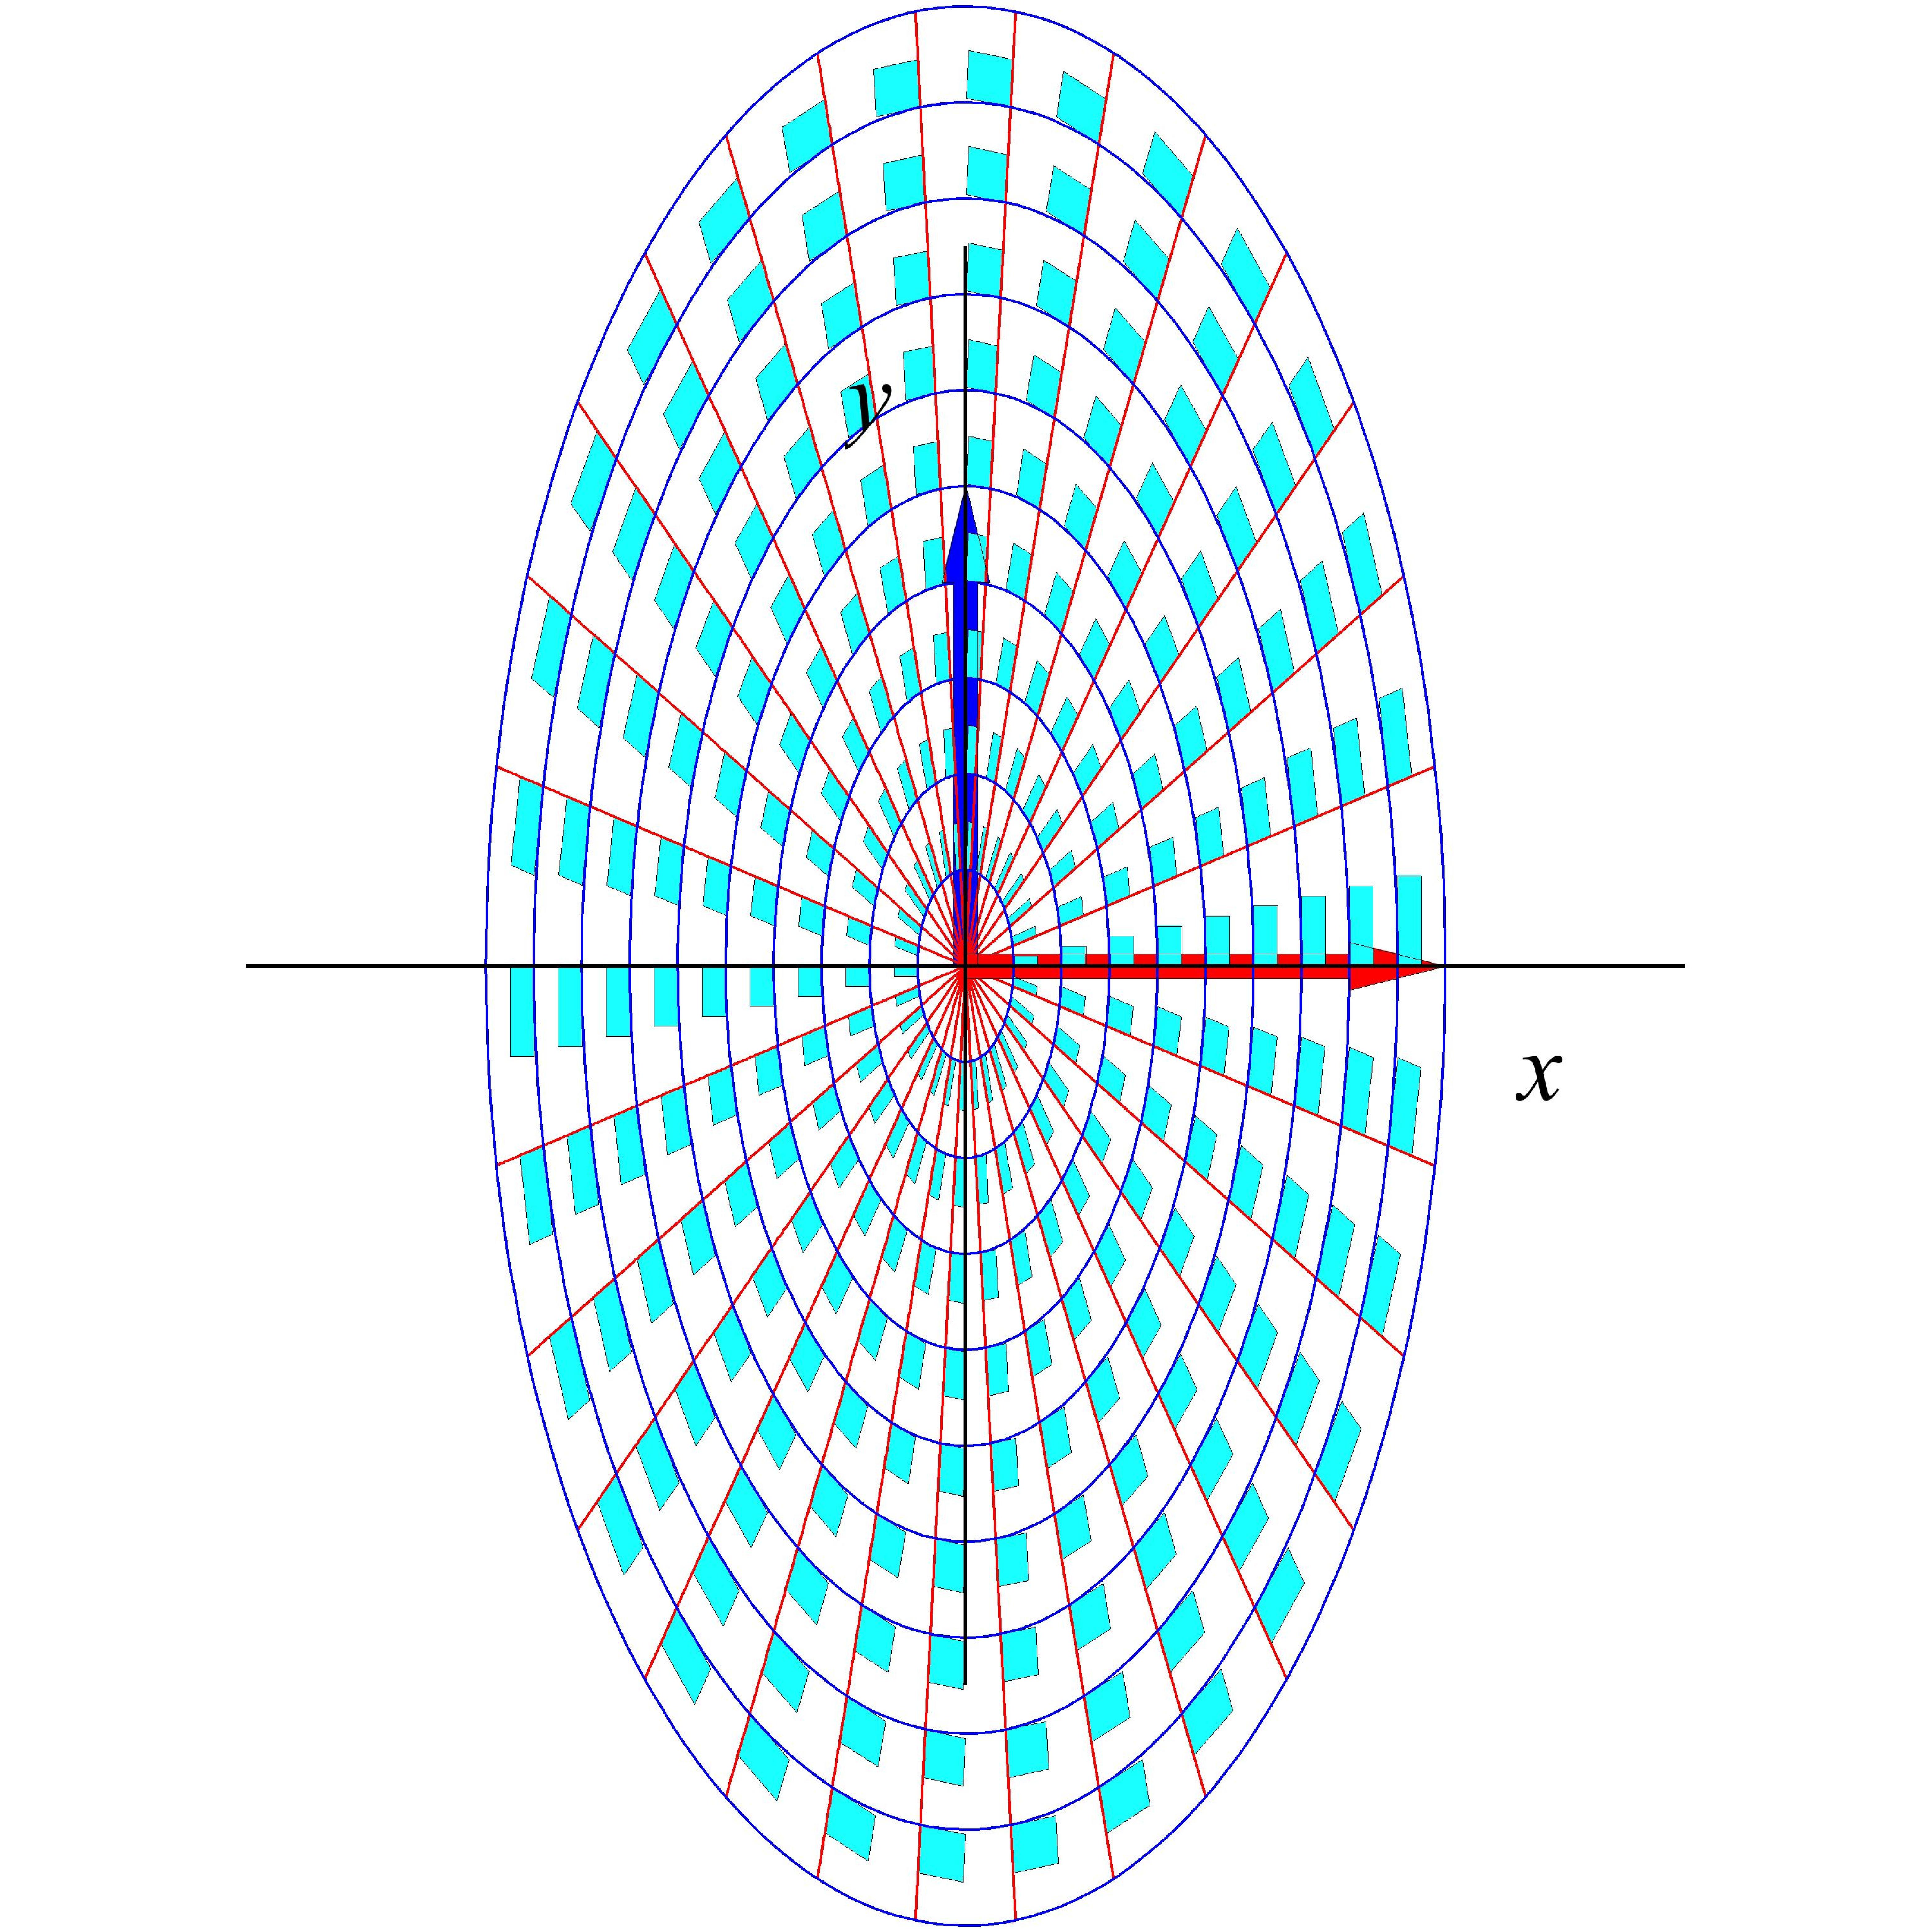
\includegraphics[height=60mm]{FIGS/plotEllipseDisk}}
\begin{center}
\caption{\small{Et elliptisk område i planen med halvakser $a=1$ og $b=2$. Se
eksempel \ref{exEllipseDisk}.
Bemærk, at de approksimerende parallelogrammer (her vist skalerede) ikke er rektangler.}} \label{figEllipseDisk}
\end{center}
\end{figure}

\begin{exercise}[Niveau-afgrænset elliptisk område] \label{exercEllipseLevel}
Et elliptisk område i planen er afgrænset af niveaukurven $\mathcal{K}_{0}(f)$ for andengradspolynomiet
\begin{equation}
f(x,y) = 2\cdot x^{2} + 2\cdot y^{2} + 2\cdot x\cdot y -8\cdot x -10 \cdot y + 13 \quad.
\end{equation}
Bestem længden af niveukurven og bestem arealet af det afgrænsede elliptiske område i $(x,y)$-planen. Se figur \ref{figEllipseLevel}. Vink: \tref{NUID35-exampEllip01}{eksempel} i \tref{NUID35-tn20}{eNote}.
\end{exercise}

\begin{figure}[ht]
\centerline{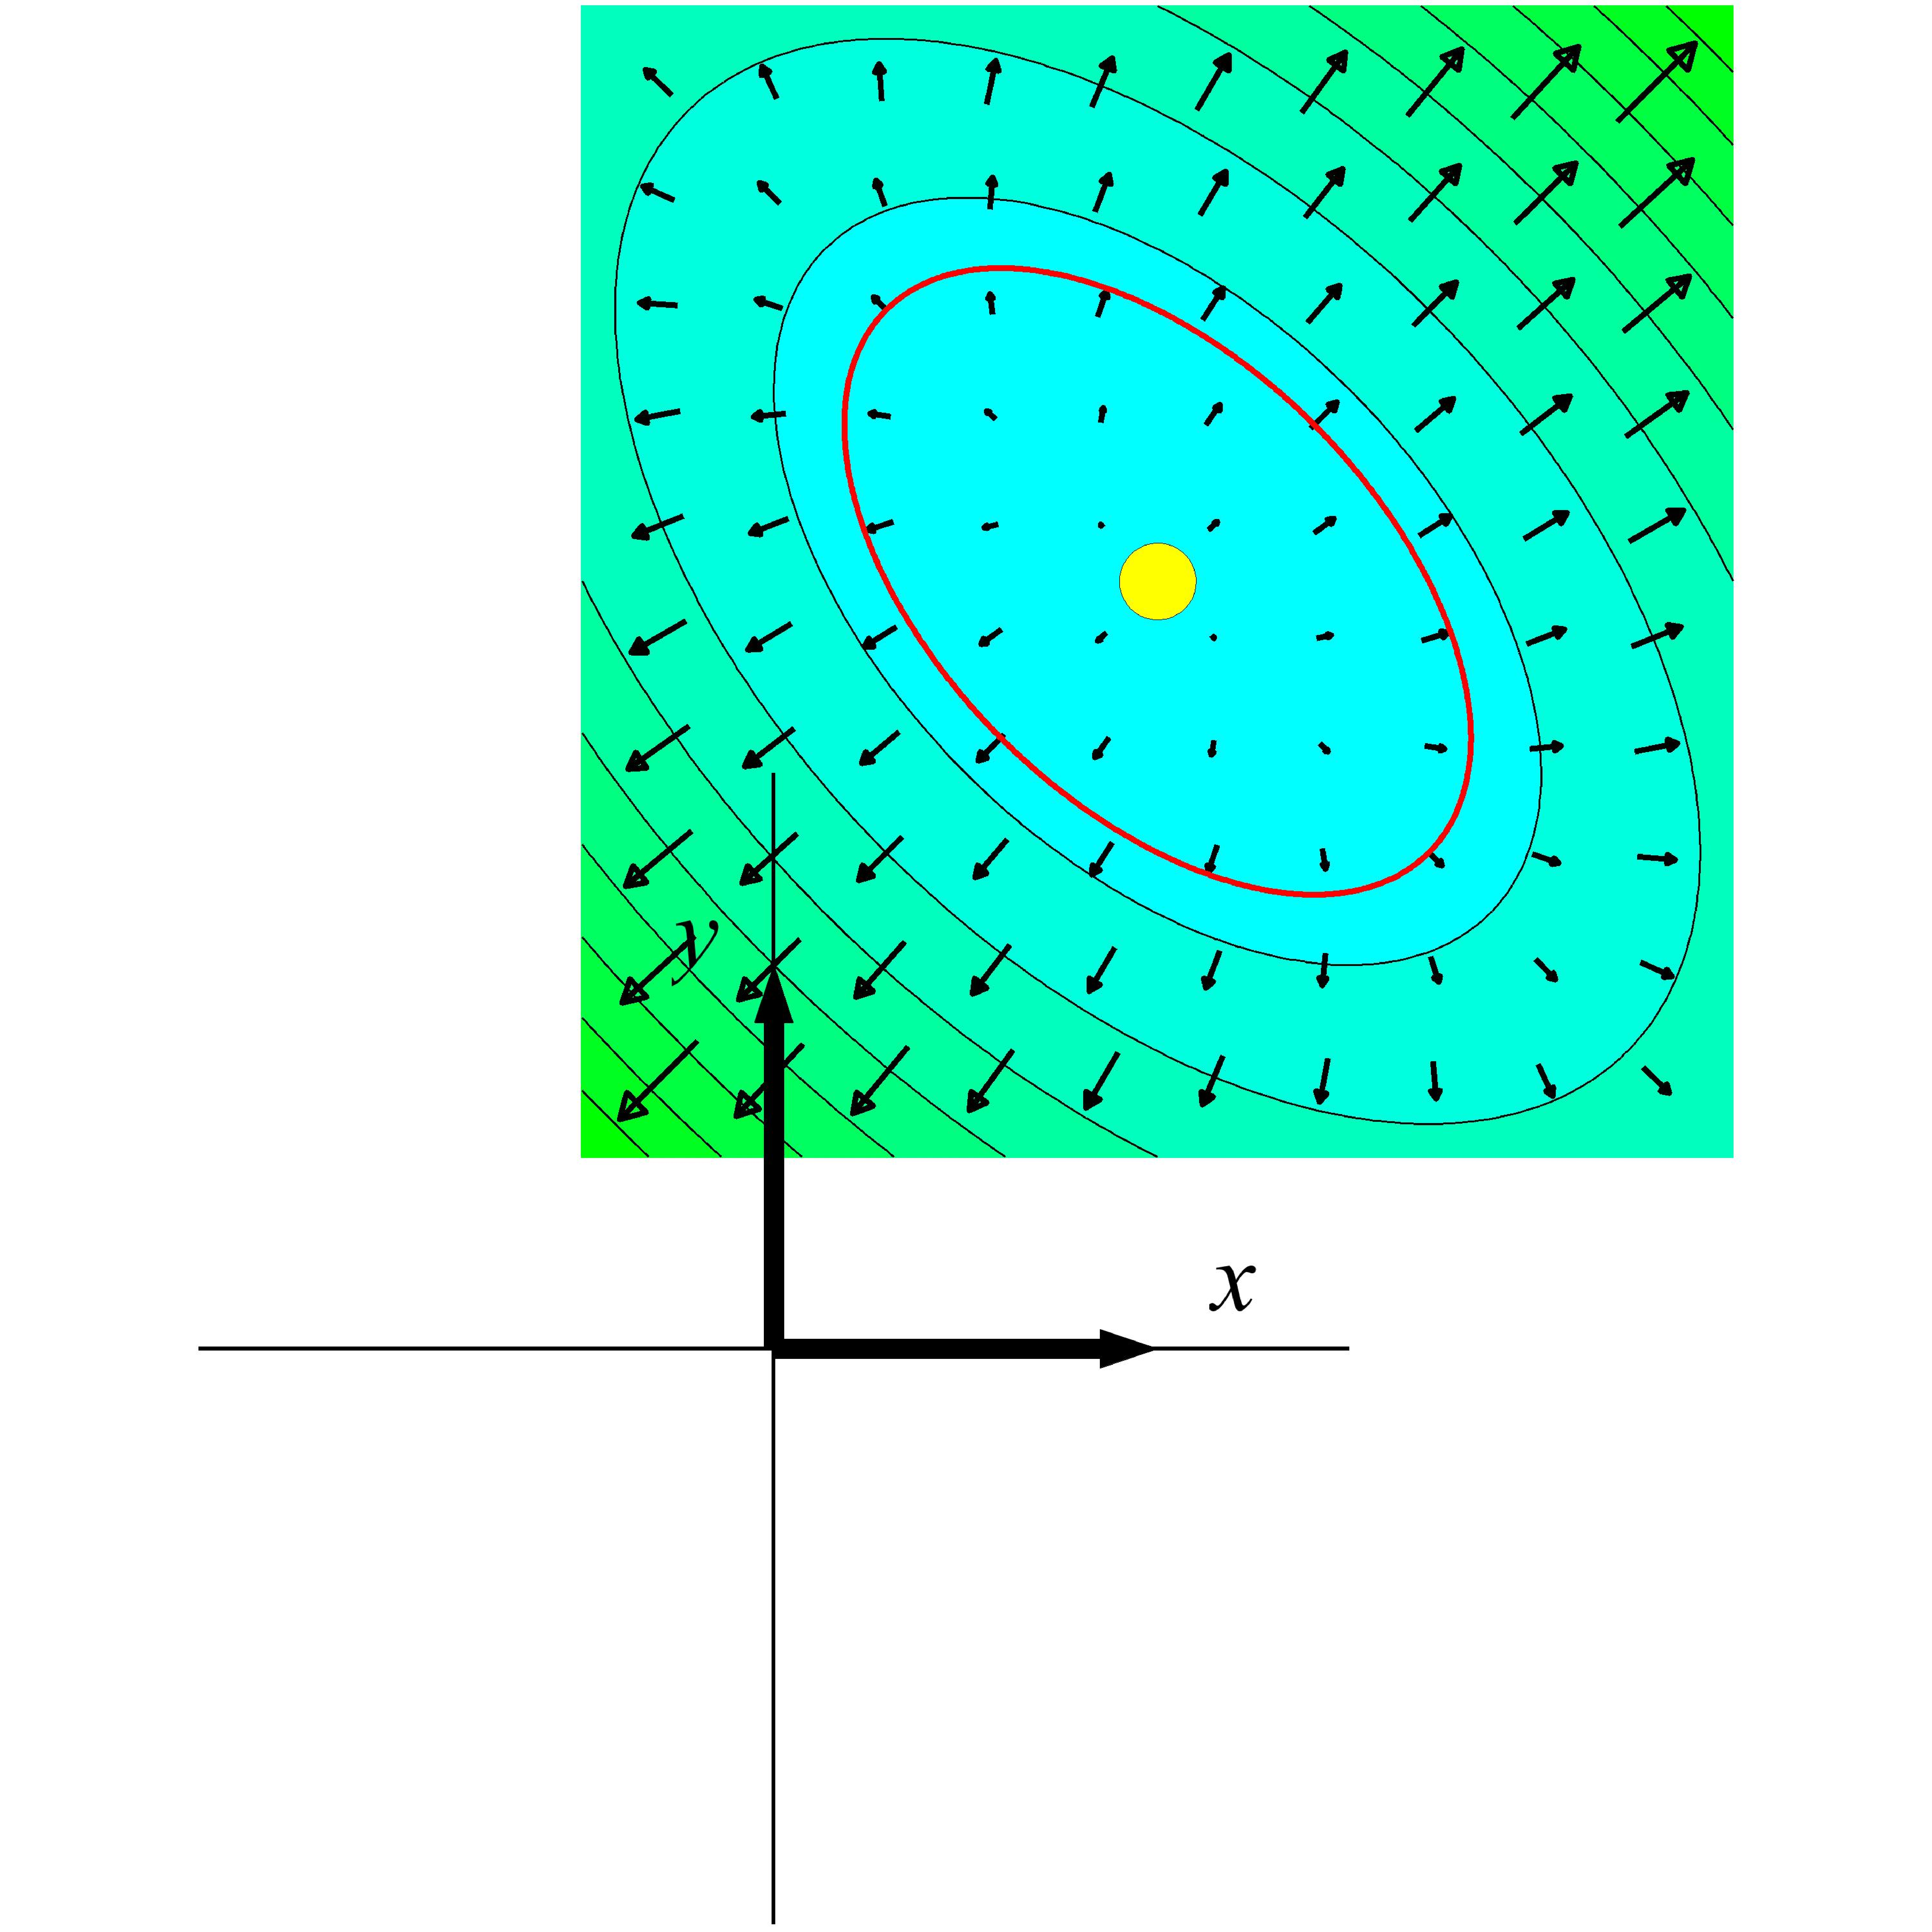
\includegraphics[height=60mm]{FIGS/plot2DGradEllip01}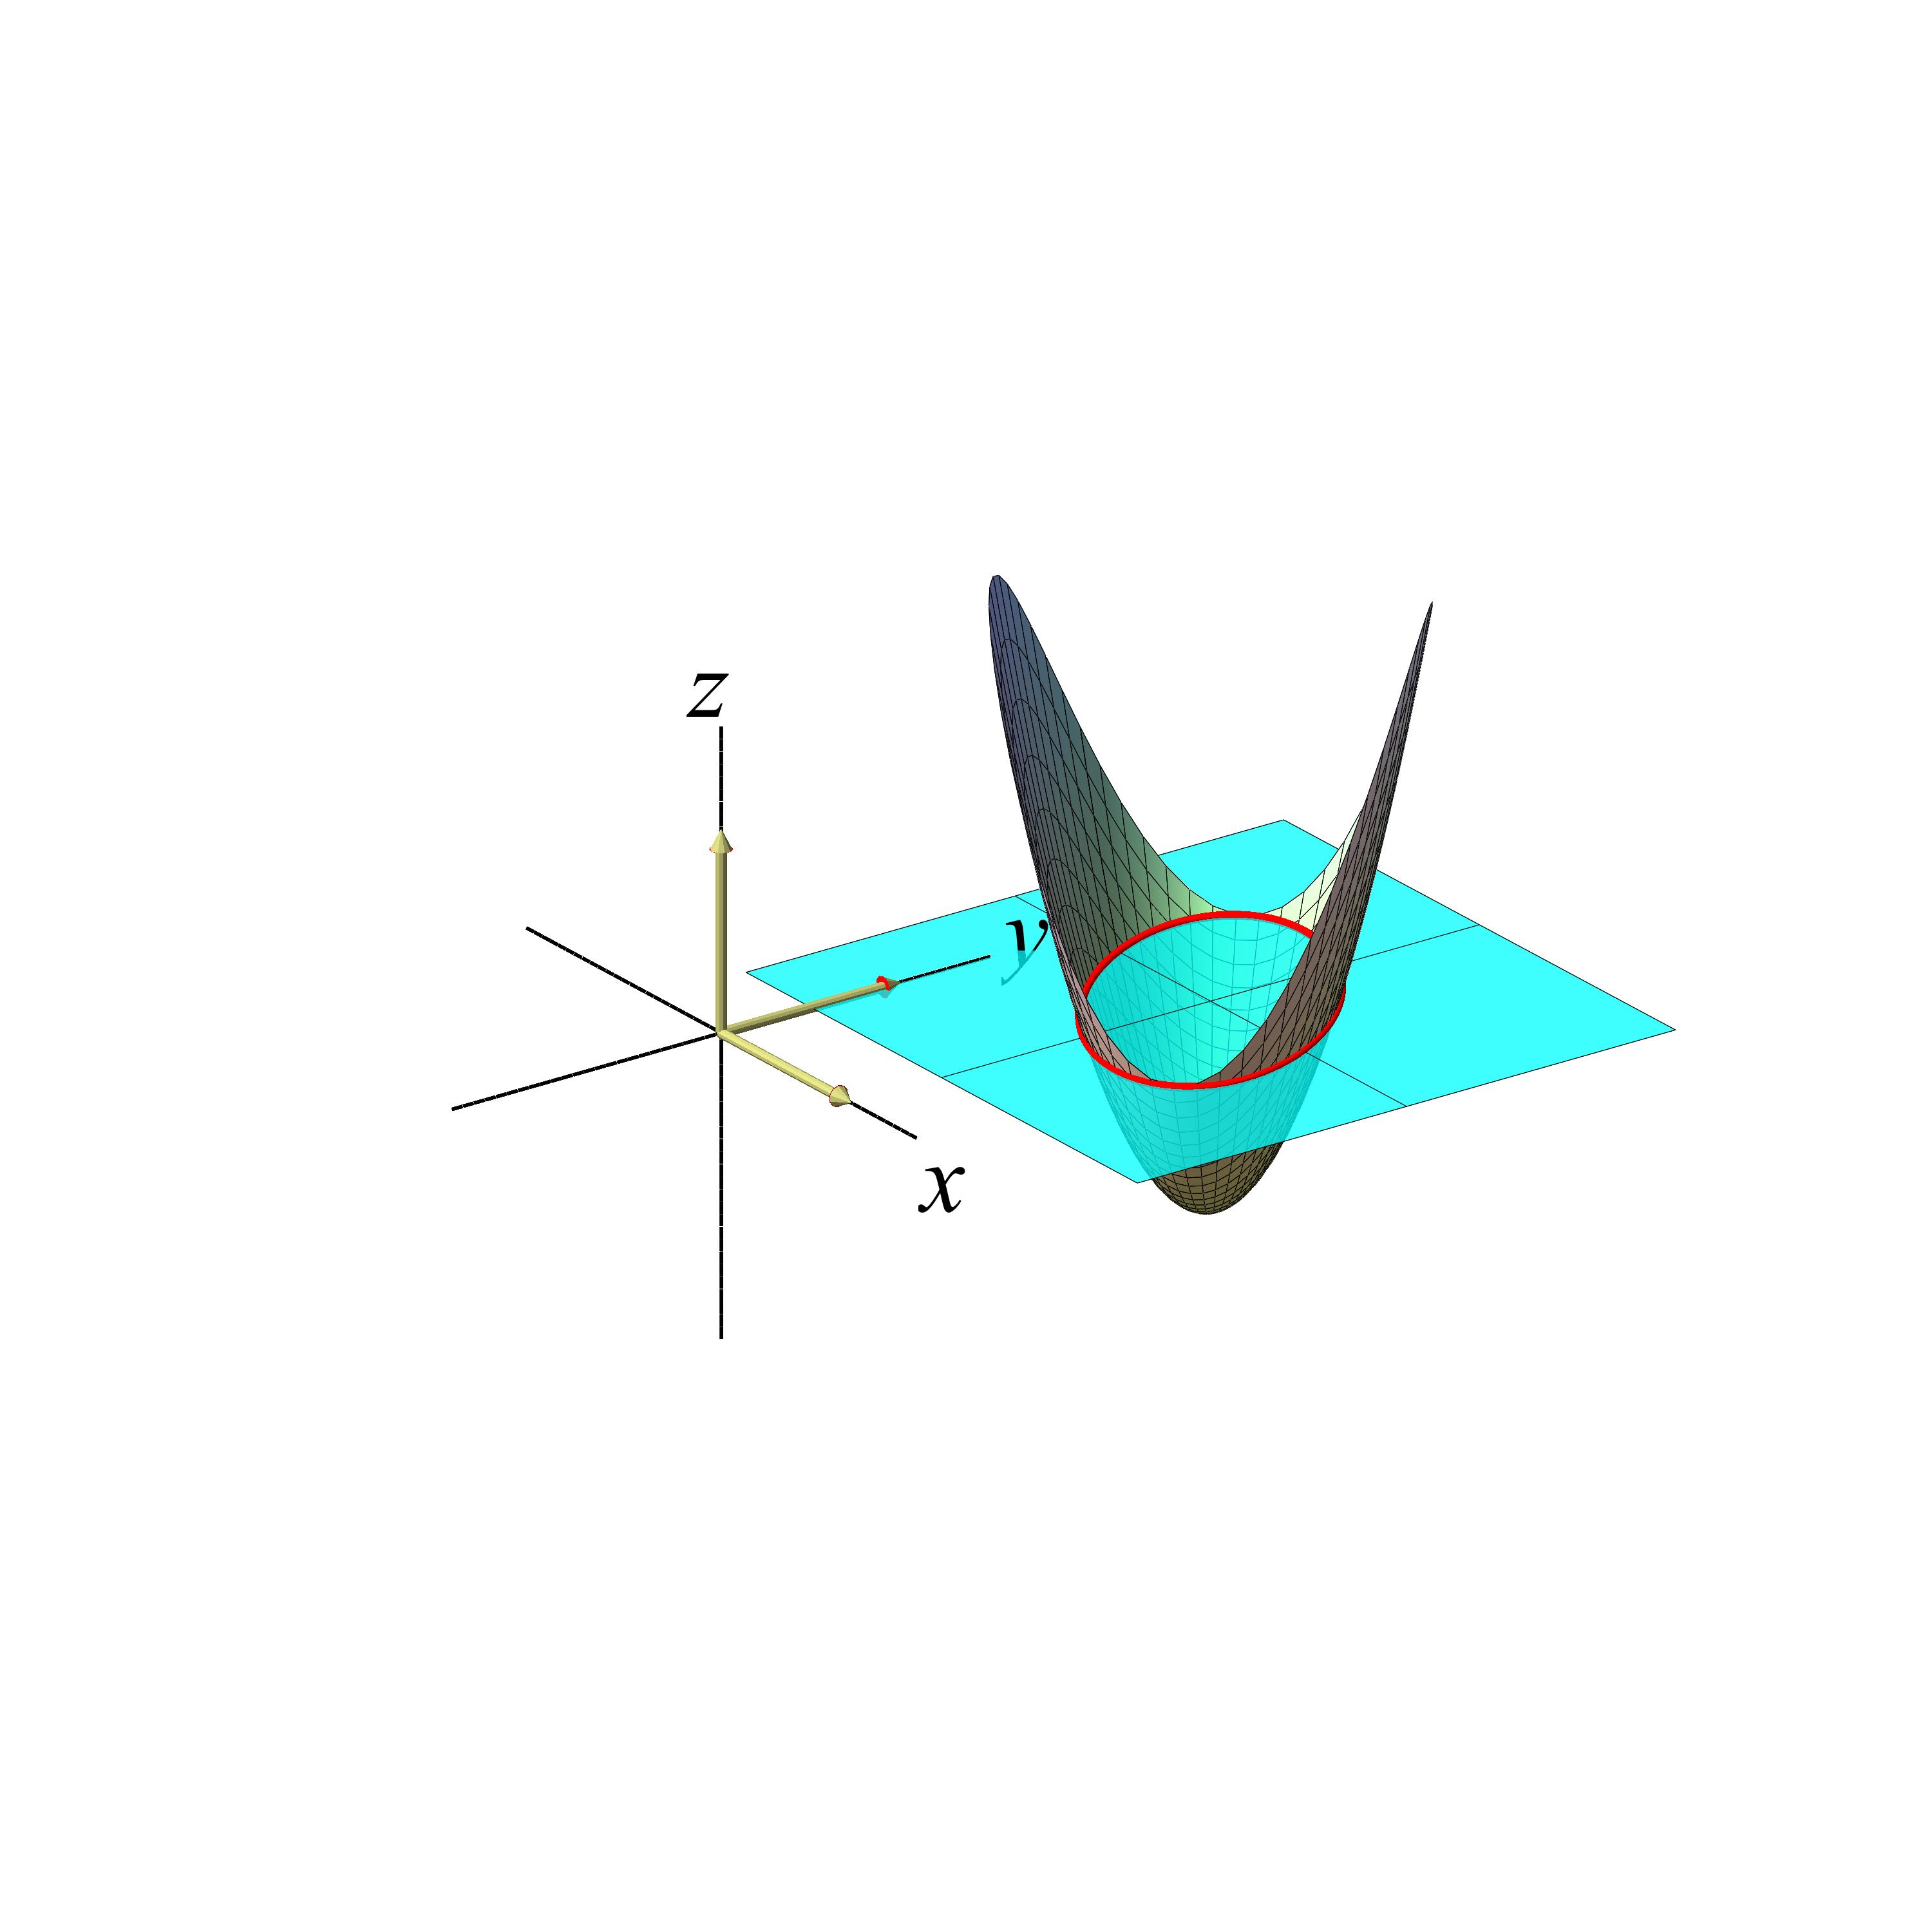
\includegraphics[height=60mm]{FIGS/plot2DNivEllipLift01} }
\begin{center}
\caption{\small{Et elliptisk område i planen er afgrænset af en ellipse som er niveaukurven $\mathcal{K}_{0}(f)$ for andengradspolynomiet $f(x,y) = 2\cdot x^{2} + 2\cdot y^{2} + 2\cdot x\cdot y -8\cdot x -10 \cdot y + 13$. Se opgave \ref{exercEllipseLevel}  og  \tref{NUID35-exampEllip01}{eksempel} i \tref{NUID35-tn20}{eNote}.}} \label{figEllipseLevel}
\end{center}
\end{figure}







\begin{example}[Spiral-område] \label{exSpiralFill}
Det parametriserede spiral-afgrænsede område i planen (se Figur \ref{figSpiralFill})
$$
P_{\bf r}: \,\, {\bf
r}(u, v) \, = \, \left(\, vu\cos(u), \,vu\sin(u) \, \right) \, , \, \, u \in
[\,0, \pi/2] \, \, , \, \, v \in [\,0, 1] \, .
$$
har arealet
$$
\Ar(P_{\bf r}) \, = \, \int_{P_{\bf r}} 1 \, d\mu \, = \,
\int_{0}^{1} \int_{0}^{\pi/2} \,\, v^{2}u \,\,du  \,\, dv \\
  \, = \,  \pi^{3}/48\quad,
$$
idet $\Jac_{\bf r}(u,v)\,= \, v^{2}u\,$. Sammenlign med beregningen af {\em{længden af spiralen}} i
eksempel \ref{exSpiral}.

\end{example}

\begin{figure}[ht]
\centerline{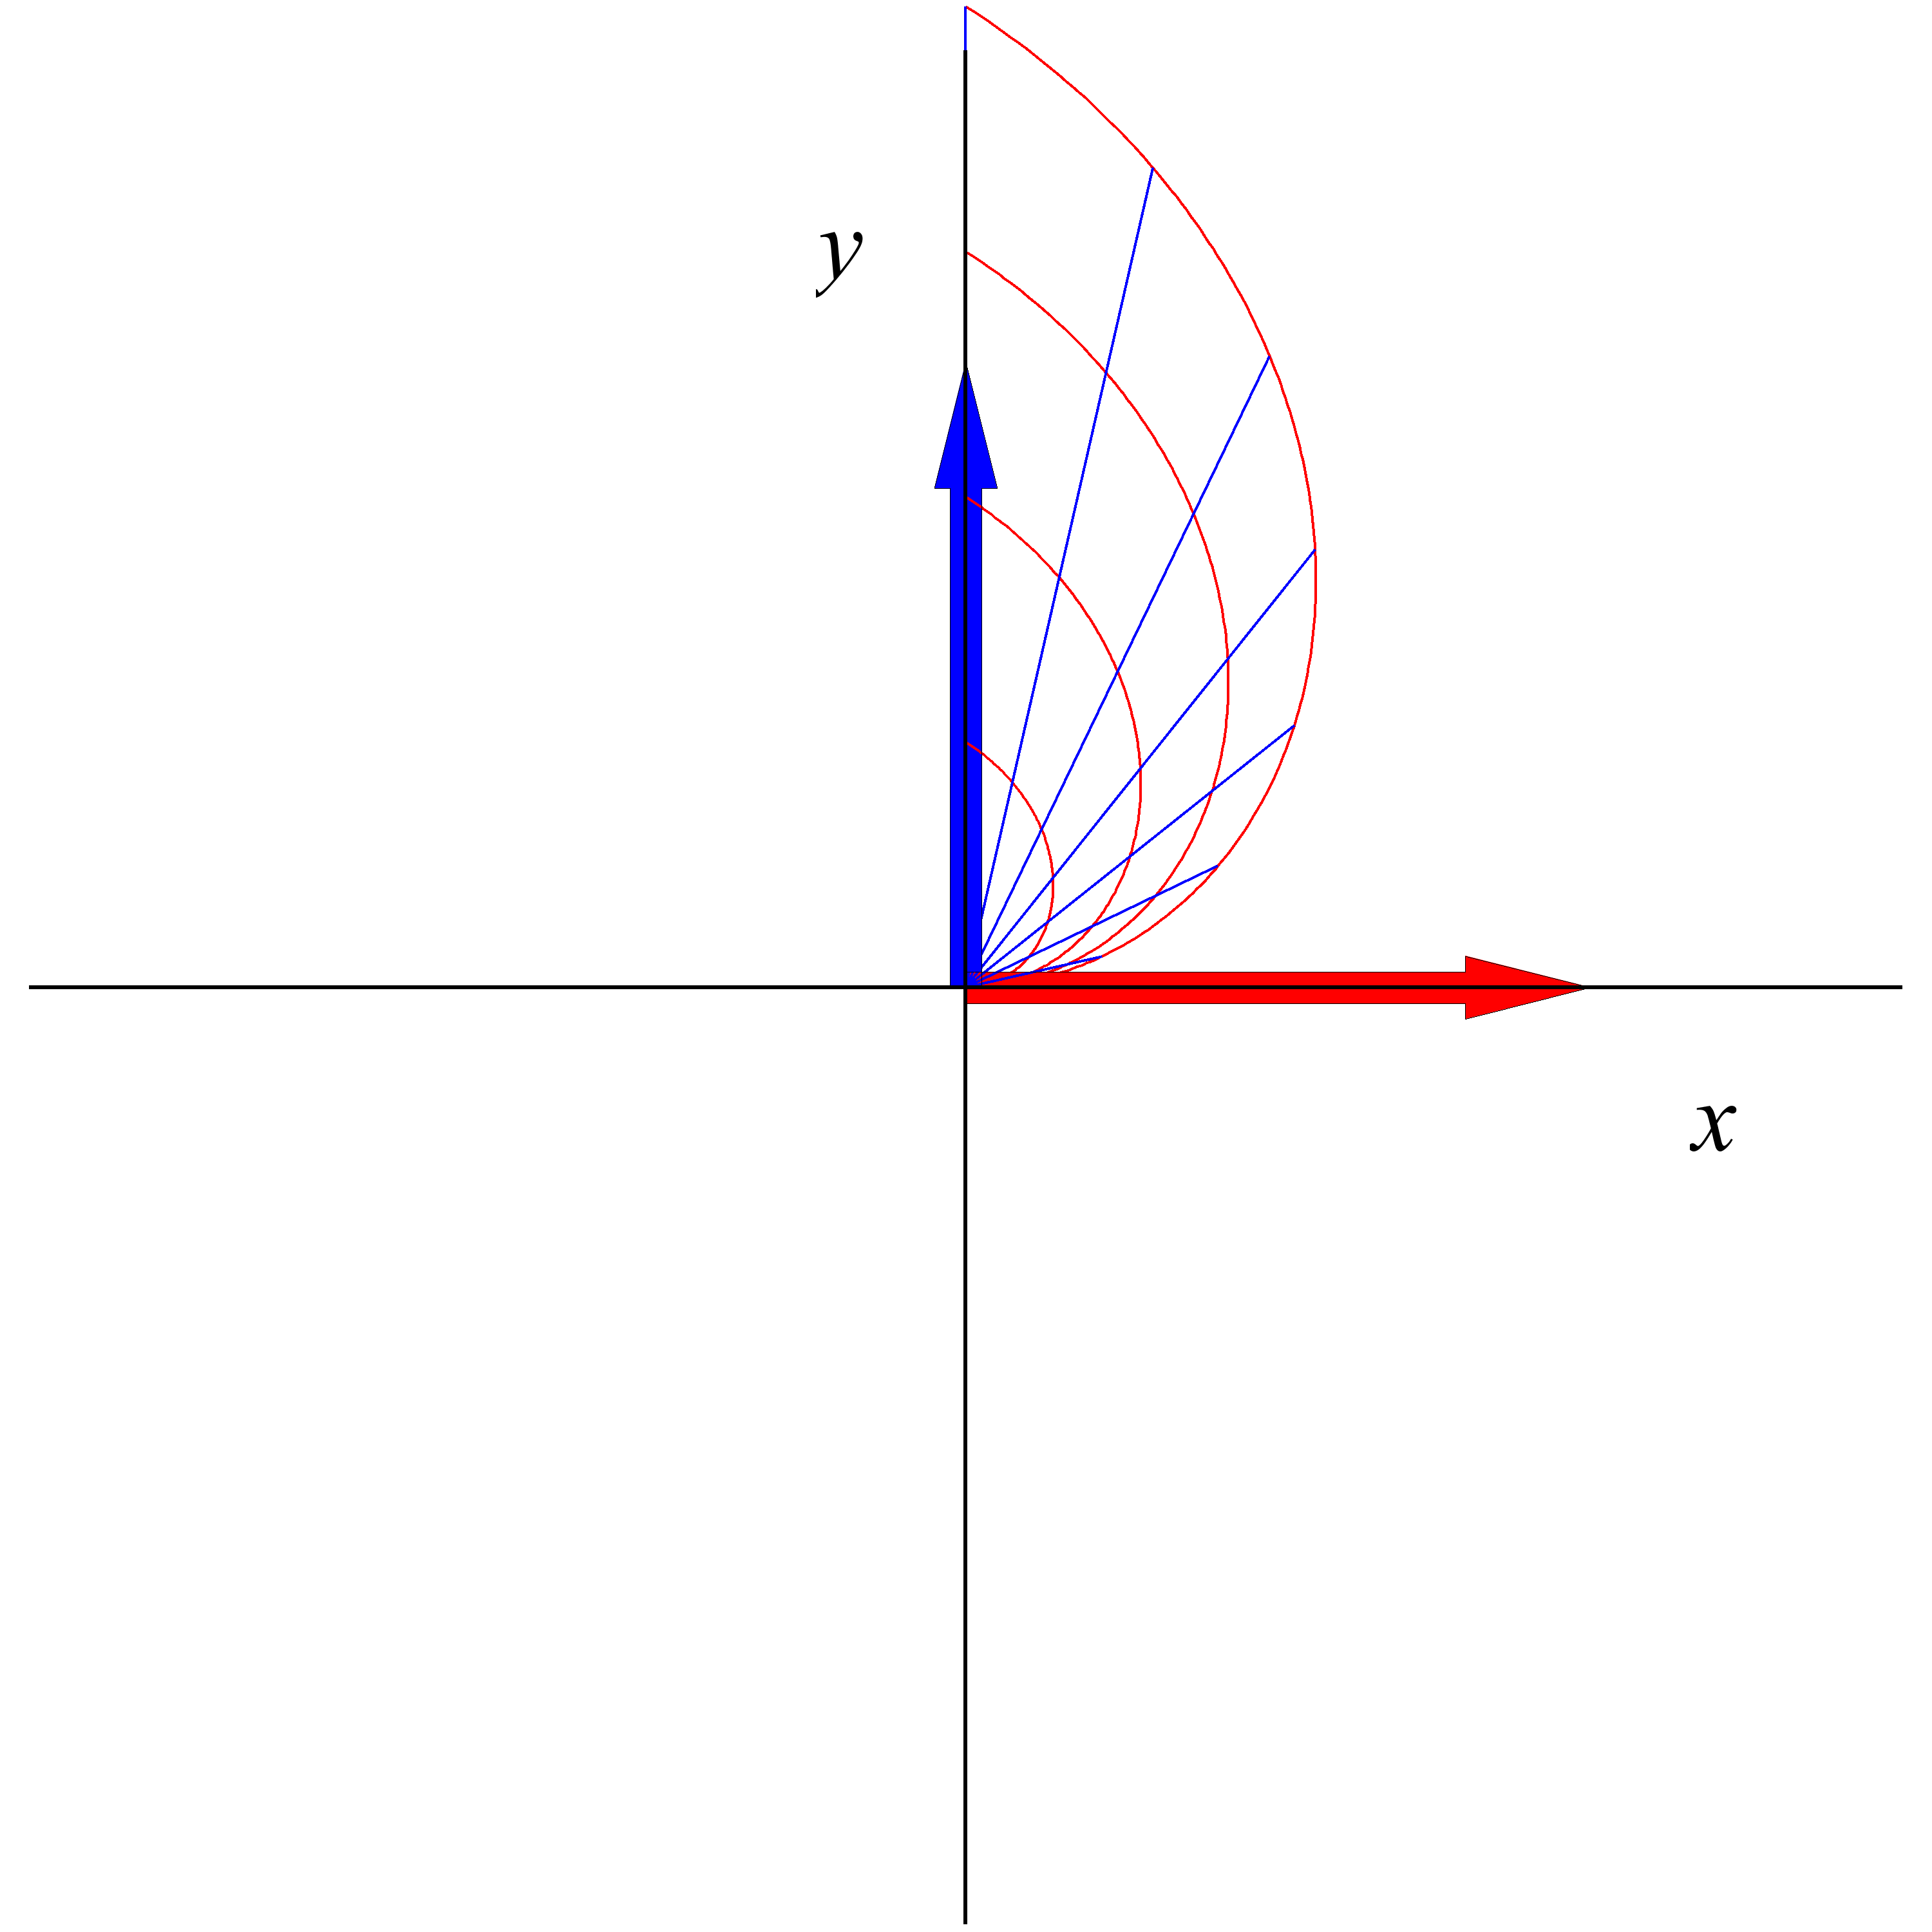
\includegraphics[height=70mm]{FIGS/plotSpiralFill}\,\,\, 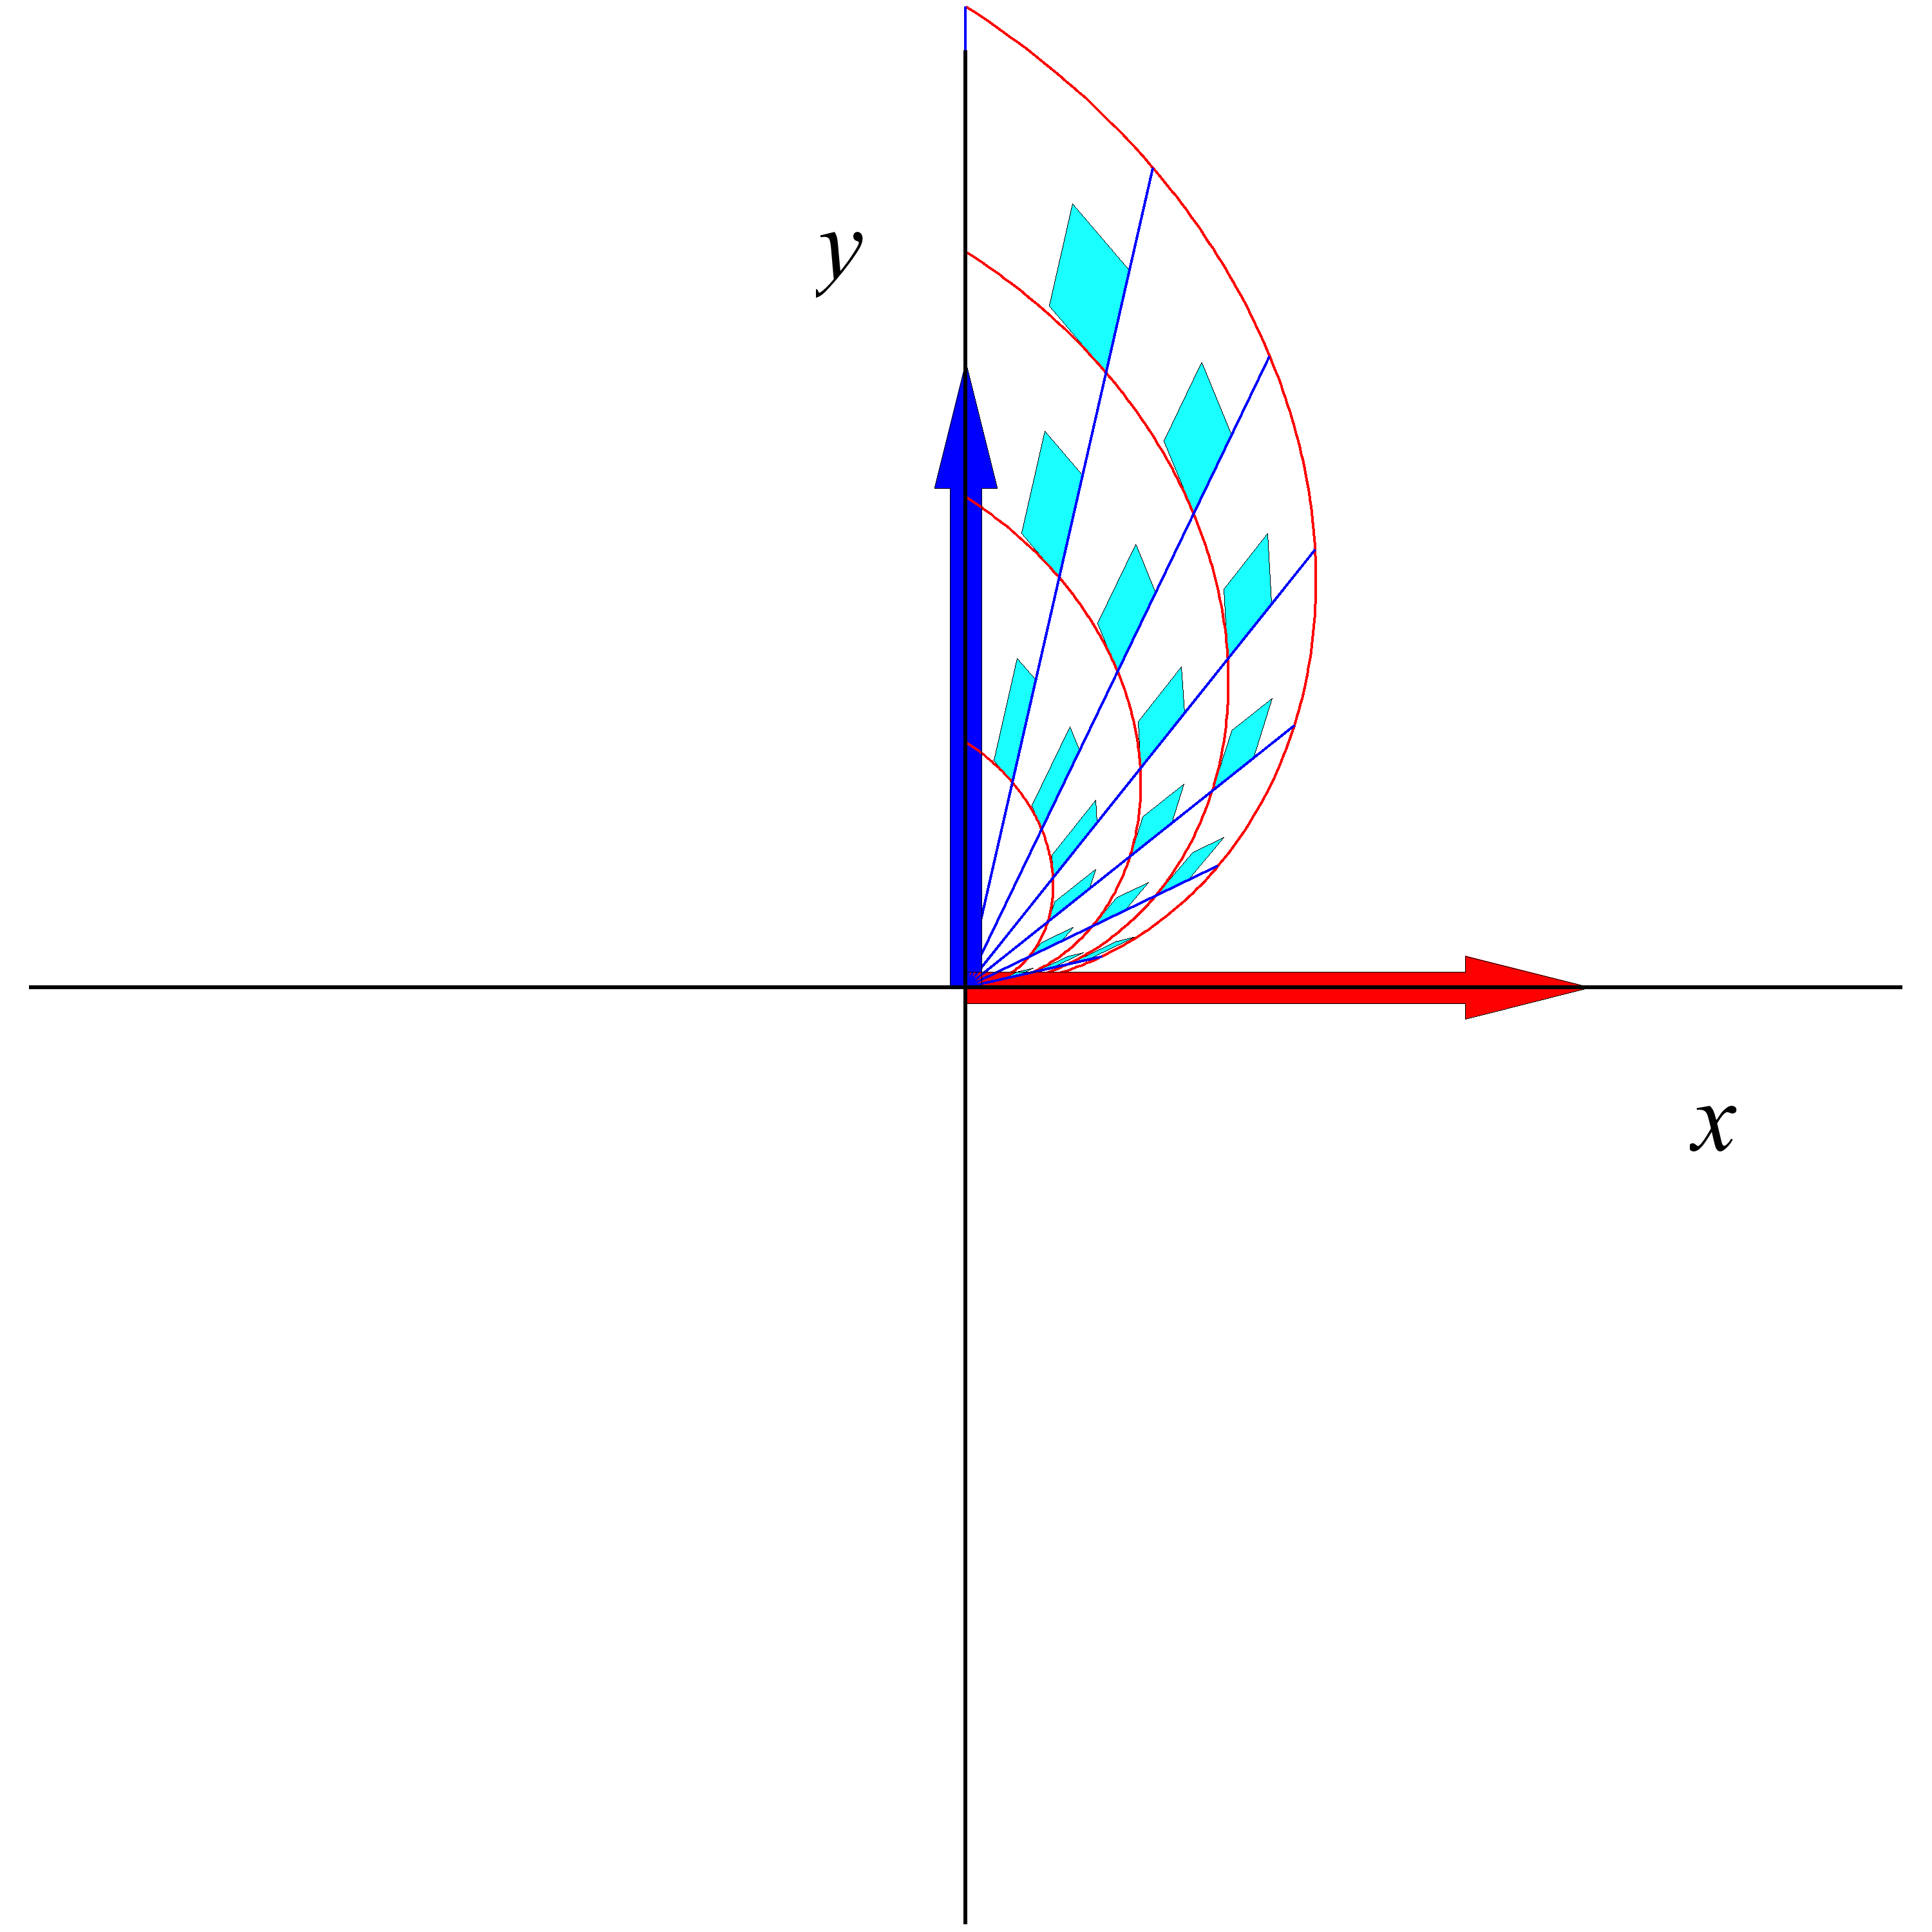
\includegraphics[height=70mm]{FIGS/plotSpiralFillApproks}}
\begin{center}
\caption{\small{Et spiral-afgrænset område i planen. Se
eksempel \ref{exSpiralFill}. }} \label{figSpiralFill}
\end{center}
\end{figure}


%%%%%%%%%%%%%%%%%%%%%%%%%%%%%%%%%%%%%%%%%%%%%%%%%%%
%%%%%%%%%%%%%%%%%%%%%%%%%%%%%%%%%%%%%%%%%%%%%%%%%%%
%%%%%%%%%%%%%%%%%%%%%%%%%%%%%%%%%%%%%%%%%%%%%%%%%%%


\subsection{Motivering af plan-integralet} \label{secMotivPlanInt}

Hvis vi i analogi med opstillingen af kurveintegralet deler {\em begge}
parameter-intervallerne $[a, b]$ og
 $[c, d]$ i henholdsvis $n$ og $m$
lige store dele, så har hvert $u$-delinterval længden $\delta_{u} \,
= \, (b-a)/n$ og hvert $v$-delinterval har længden $\delta_{v} \, =
\, (d-c)/m$. Tilsvarende bliver delepunkternes koordinater i $(u,
v)$-parameterområdet (som jo er rektanglet $[a,b]\times[c,d]$ i
$\mathbb{R}^{2}\,$) - jvf. \tref{NUID35-tn20}{eNote}:

\begin{equation}
\begin{aligned}
(u_{1}, v_{1}) \, &= \, (a, c), \\
(u_{1}, v_{j}) \, &= \, (a, c + (j-1)\delta_{v}), \\
(u_{i}, v_{1}) \, &= \, (a + (i-1)\delta_{u}, c), \\
(u_{i}, v_{j}) \, &= \, (a + (i-1)\delta_{u}, c + (j-1)\delta_{v}), \\
 &.... \\
(b, d) \, &= \, (a + n\delta_{u}, c + m\delta_{v}) \quad .
\end{aligned}
\end{equation}

Med hvert af disse faste punkter $(u_{i}, v_{j})$ som udviklingspunkt kan vi igen
benytte Taylor's grænseformel, nu for hver af de $2$  koordinat-funktioner $x(u,v)$ og $y(u,v)$  for $\,{\bf r}(u,
v) \, = \, \left(x(u,v), y(u,v)\right)\, $ til første orden med tilhørende epsilon-funktioner:
\begin{equation} \label{eqTaylor2}
\begin{aligned}
{\bf r}(u, v) \, = \, {\bf r}(& u_{i}, v_{j}) \\
+ \, &{\bf r}'_{u}(u_{i}, v_{j})\cdot(u-u_{i}) \\
+ \, &{\bf r}'_{v}(u_{i}, v_{j})\cdot(v-v_{j}) \\
+ \, &\rho_{ij}\cdot {\bm{\varepsilon}}_{ij}(u-u_{i}, v-v_{i}) \quad
,
\end{aligned}
\end{equation}
hvor  $\, u\, \, \in\, \left[\, u_{i}\, , \,  u_{i} +
\delta_{u}\,\right]\, , \,\, v\, \, \in\, \left[\, v_{j}\, , \,
v_{j} + \delta_{v}\,\right] .$ Her betegner  $\, \rho_{ij} =
\sqrt{(u - u_{i})^{2} + (v - v_{j})^{2}}\, $ afstanden mellem det
variable punkt $\,(u\,, v)\,$ og det faste udviklingspunkt
$\,(u_{i}\,,v_{j})\,$ i parameterområdet. Der gælder her, at vektorfunktionen
$\,{\bm{\varepsilon}}_{ij}(u-u_{i}, v-v_{j}) \to (0, 0)\, = \
{\bf{0}}\,$ for $\,(u-u_{i}, v-v_{j}) \to (0, 0)\,$ . \\


Hvert del-rektangel $[u_{i}, u_{i}+\delta_{u}]\times[v_{j},
v_{j}+\delta_{v}]$ afbildes på det plane del-område, som vi kan angive med ${\bf r}(u,v)$ evalueret i parameter-del-rektanglet
$u \in[u_{i}, u_{i}+\delta_{u}], v \in[v_{j}, v_{j}+\delta_{v}]$ og
dette delområde af det plane område kan vi approksimere med den lineære del af
udtrykket i (\ref{eqTaylor2}), som igen netop fås ved at fjerne
${\bm{\varepsilon}}_{ij}$-bidraget fra højre side i
(\ref{eqTaylor2}):
\begin{equation}\label{eqApp2}
{\bf r}_{\app_{\,ij}}(u, v) \, = \, {\bf r}(u_{i}, v_{j}) + \, {\bf
r}'_{u}(u_{i}, v_{j})\cdot (u - u_{i}) + \, {\bf r}'_{v}(u_{i},
v_{j})\cdot (v - v_{j}) \quad ,
\end{equation}
hvor $u$ og $v$ stadig gennemløber del-intervallerne $\, u\, \,
\in\, \left[\, u_{i}\, , \,  u_{i} + \delta_{u}\,\right]\, , \,\,
v\, \, \in\, \left[\, v_{j}\, , \, v_{j} + \delta_{v}\,\right] .$


 Disse lineære approksimationer er parallelogrammer,
som udspændes af de to tangentvektorer ${\bf
r}'_{u}(u_{i}, v_{j})\cdot\delta_{u}$ og ${\bf
r}'_{v}(u_{i}, v_{j})\cdot \delta_{v}$.


\subsubsection{Areal af plant område} \label{subsecArealPlan}
Hvert enkelt af de ialt $n\cdot m$ approksimerende
parallelogrammer har et areal. Arealet af det
$(i, j)$'te parallelogram er givet ved

\begin{equation}
\begin{aligned}
\Delta \Ar_{ij} \, &= \,  | {\bf r}'_{u}(u_{i},v_{j}) | \cdot | {\bf
r}'_{v}(u_{i},v_{j}) | \, \sin(\theta(u_{i},v_{j}))\cdot  \delta_{u}\cdot \delta_{v} \, \\
&= \, \Jac_{\bf r}(u_{i}, v_{j})\cdot \delta_{u}\cdot \delta_{v} \quad.
\end{aligned}
\end{equation}



\begin{exercise}
Bevis denne påstand: Arealet af et parallelogram
er produktet af længderne af de to udspændende vektorer og sinus til den mellemliggende vinkel.
Se \tref{NUID12-tn6}{eNote}
\end{exercise}


Summen af disse ialt $n\,m$ arealer er klart en god approksimation
til arealet af hele fladestykket, således at vi har
\begin{equation}
\Ar_{\app}(n,m)\, = \,   \sum_{j=1}^{m}\sum_{i=1}^{n} \Delta \Ar_{ij}
\, = \,  \sum_{j=1}^{m}\sum_{i=1}^{n} \Jac_{\bf r}(u_{i},
v_{j})\cdot \delta_{u} \delta_{v}  \quad.
\end{equation}
Da ovenstående sum er en dobbelt integralsum for den kontinuerte
funktion $\, \Jac_{\bf r}(u, v)\, $ over parameter-rektanglet $\,
[a, b]\times[c, d]\, $ får vi i grænsen, hvor $n$ og $m$ begge går
mod uendelig (se \tref{NUID36-tn21}{eNote} ):
\begin{equation}
\Ar_{\app}(n,m)\,  \to \, \Ar\, = \, \int_{c}^{d} \int_{a}^{b}
\Jac_{\bf r}(u, v) \,du \, dv \quad \text{for} \quad n\, , \, m  \to
\infty \quad.
\end{equation}

Dette er begrundelsen for definitionen af arealet af et
parametriseret område i planen som angivet ovenfor, nemlig som
fladeintegralet af den konstante funktion $1$.






\subsubsection{Massen, vægten af et plant område} \label{subsecMassPlant}

Hvis vi nu antager, at
hvert enkelt parallelogram i (\ref{eqApp2})
tildeles en konstant massetæthed givet ved
værdien af funktionen $f(x,y)$ i
parallelogrammets kontaktpunkt med fladen, så får
vi massen af det $(i, j)$'te parallelogram :
\begin{equation}
\begin{aligned}
\Delta \M_{ij} \, &= \, f(x(u_{i}, v_{j}), y(u_{i}, v_{j})) \, \Jac_{\bf r}(u_{i}, v_{j}) \cdot\delta_{u} \delta_{v} \, \\
&= \, f( {\bf r}(u_{i}, v_{j})) \, \Jac_{\bf r}(u_{i}, v_{j})
\cdot\delta_{u} \delta_{v}\quad .
\end{aligned}
\end{equation}
Den totale masse af hele systemet af
parallelogrammer er derfor følgende, som er en
god ap\-proksimation til massen af hele det plane område
når dette gives massetætheden $f({\bf r}(u,v))$ i
punktet ${\bf r}(u,v)$.
\begin{equation}
\M_{\app}(n,m) \, = \,  \sum_{j=1}^{m} \sum_{i=1}^{n} \Delta \M_{ij} \,
= \, \sum_{j=1}^{m}\sum_{i=1}^{n}f({\bf r}(u_{i},
v_{j}))\,\Jac_{\bf r}(u_{i}, v_{j}) \cdot \delta_{u} \delta_{v}
\quad .
\end{equation}

Dette er en dobbelt integralsum for den kontinuerte funktion $f({\bf
r}(u,v))\,\Jac_{\bf r}(u, v)$ over parameter-rektanglet $\,[a,
b]\times[c, d]\,$. Vi får altså i grænsen, hvor $n$ og $m$ går mod
uendelig:
\begin{equation}
\M_{\app}(n,m)\, \to \, \M \, = \, \int_{c}^{d}\int_{a}^{b}f({\bf r}(u,
v ))\Jac_{\bf r}(u, v)\,du \,dv \quad \text{for} \quad n\, , \, m \to
\infty \quad.
\end{equation}

Dermed har vi motiveret definitionen af massen af et
parametriseret område i planen  med massetætheden $f({\bf r}(u, v))$ og
dermed også den generelle definition af planintegralet,
definition \ref{defPlanInt}.

%%%%%%%%%%%%%%%%%%%%%%%%%%%%%%%%%%%%%%%%


%%%%%%%%%%%%%%%%%%%%%%%%%%%%%%%%%%%%%%%%%%%%%%%%%%%
%%%%%%%%%%%%%%%%%%%%%%%%%%%%%%%%%%%%%%%%%%%%%%%%%%%
%%%%%%%%%%%%%%%%%%%%%%%%%%%%%%%%%%%%%%%%%%%%%%%%%%%
%%%%%%%%%%%%%%%%%%%%%%%%%%%%%%%%%%%%%%%%%%%%%%%%%%%


\begin{example}[Total vægt af ring-område] \label{exampAnnulMass}
Lad $f(x,y) = 1+x$ være vægtfunktion på det plane område i $(x,y)$-planen der er afgrænset af $x$-aksen og de to øvre halvcirkelbuer af cirklerne med radius henholdsvis $1$ og $1/2$, begge med centrum i $(0,0)$, se figur \ref{figAnnulMass}. En parametrisering af området er for eksempel:
\begin{equation}
P_{\mathbf{r}} \quad : \quad \mathbf{r}(u,v) = (u\cdot \cos(v), u\cdot \sin(v)) \quad , \quad \textrm{hvor} \quad u \in [1/2, 1] \quad , \quad v \in [0, \pi] \quad.
\end{equation}
Når området er vægtet med vægtfunktionen $f(x,y)$ bliver den totale vægt af området:
\begin{equation}
M(P_{\mathbf{r}}) = \int_{P_{\mathbf{r}}}\, f\, d\mu = \int_{0}^{\pi}\int_{1/2}^{1} \, f(\mathbf{r}(u,v))\cdot \Jac_{\mathbf{r}}(u,v) \, du \, dv \quad ,
\end{equation}
hvor
\begin{equation}
\begin{aligned}
f(\mathbf{r}(u,v)) &= 1 + x(u,v) = 1 + u\cdot \cos(v) \quad \textrm{og} \\
\Jac_{\mathbf{r}}(u,v) &= u \quad ,
\end{aligned}
\end{equation}
sådan at
\begin{equation}
\begin{aligned}
M(P_{\mathbf{r}}) &= \int_{0}^{\pi}\int_{1/2}^{1} \,(1 + u\cdot \cos(v))\cdot u \, du \, dv \\
&= \int_{0}^{\pi}\,\left[\frac{1}{2}u^{2} + \frac{1}{3}u^{3}\cdot \cos(v)\right]_{u=1/2}^{u=1} \, dv \\
&= \int_{0}^{\pi}\, \left( \frac{3}{8} + \frac{7}{24}\cdot \cos(v) \right) \, dv \\
&= \left[ \frac{3}{8}v + \frac{7}{24}\cdot \sin(v)\right]_{v=0}^{v=\pi} \\
&= \frac{3}{8}\cdot\pi \quad .
\end{aligned}
\end{equation}
Den totale masse af området med den givne vægtfordeling er altså $M(P_{\mathbf{r}}) = 3\pi/8$. Til sammenligning er arealet af området jo også $\Ar(P_{\mathbf{r}}) = 3\pi/8$ -- men det er et tilfælde.
\end{example}

\begin{figure}[ht]
\centerline{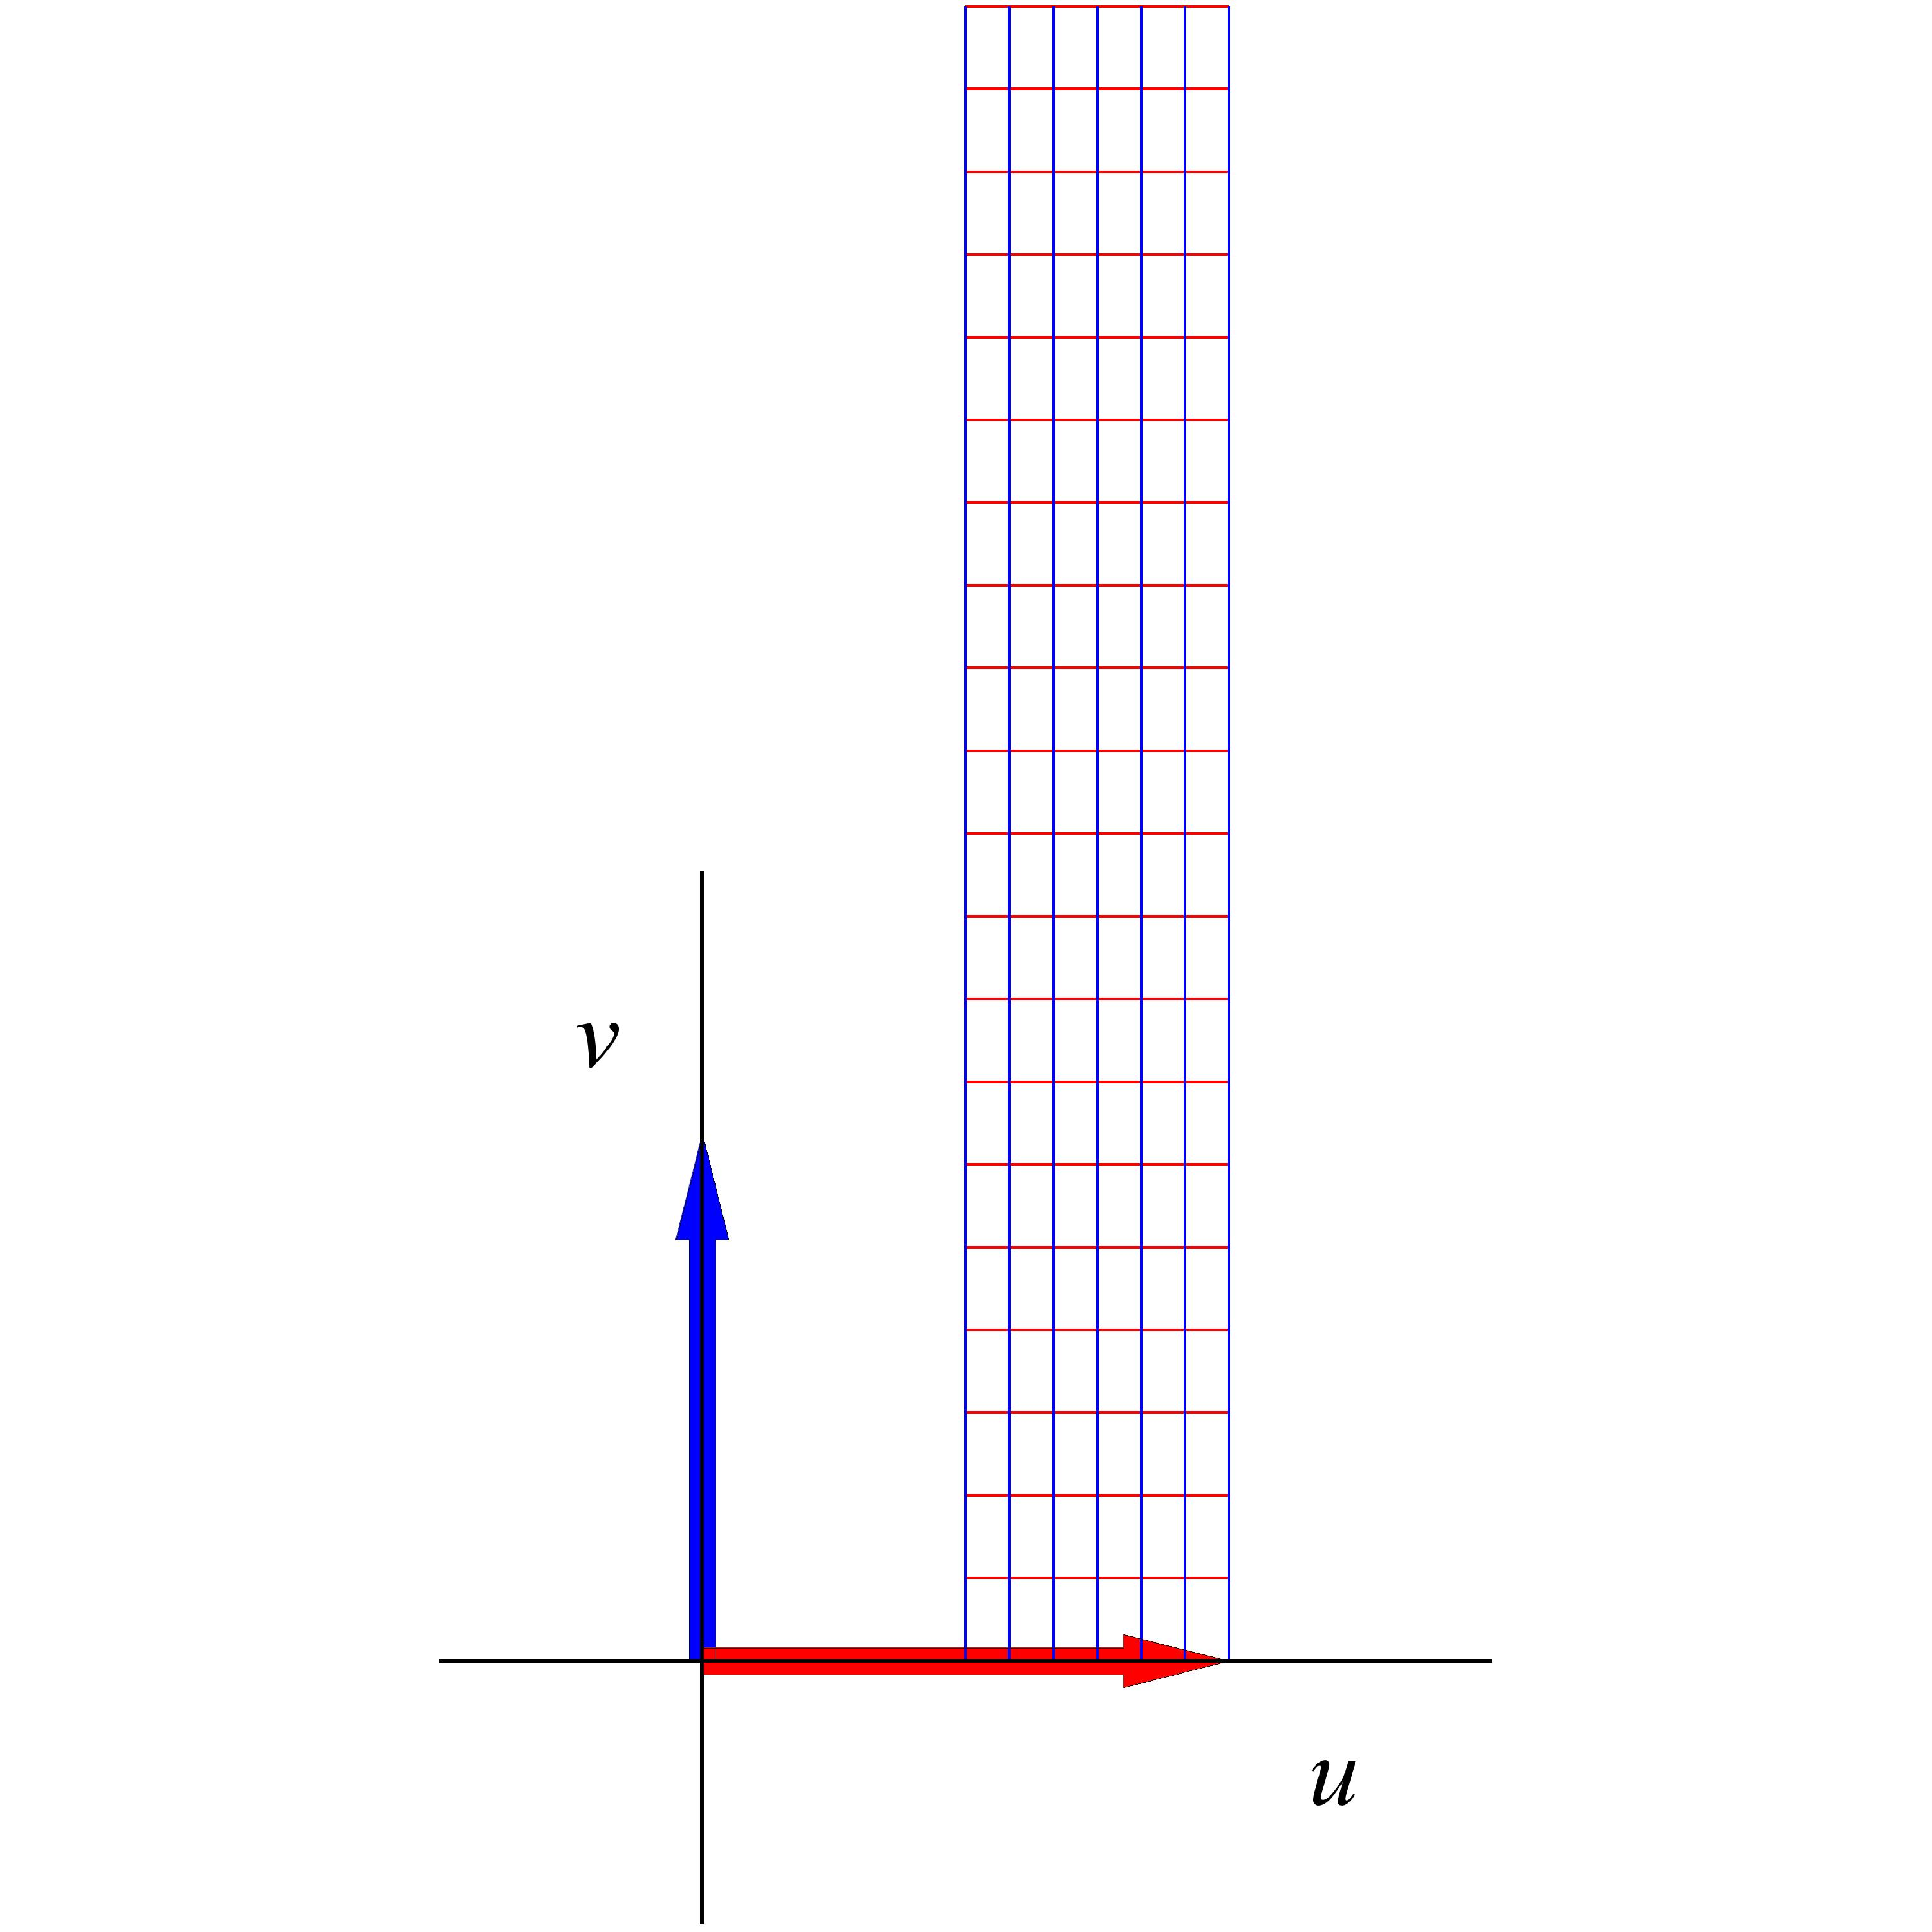
\includegraphics[height=60mm]{FIGS/plotAnnulusM1} 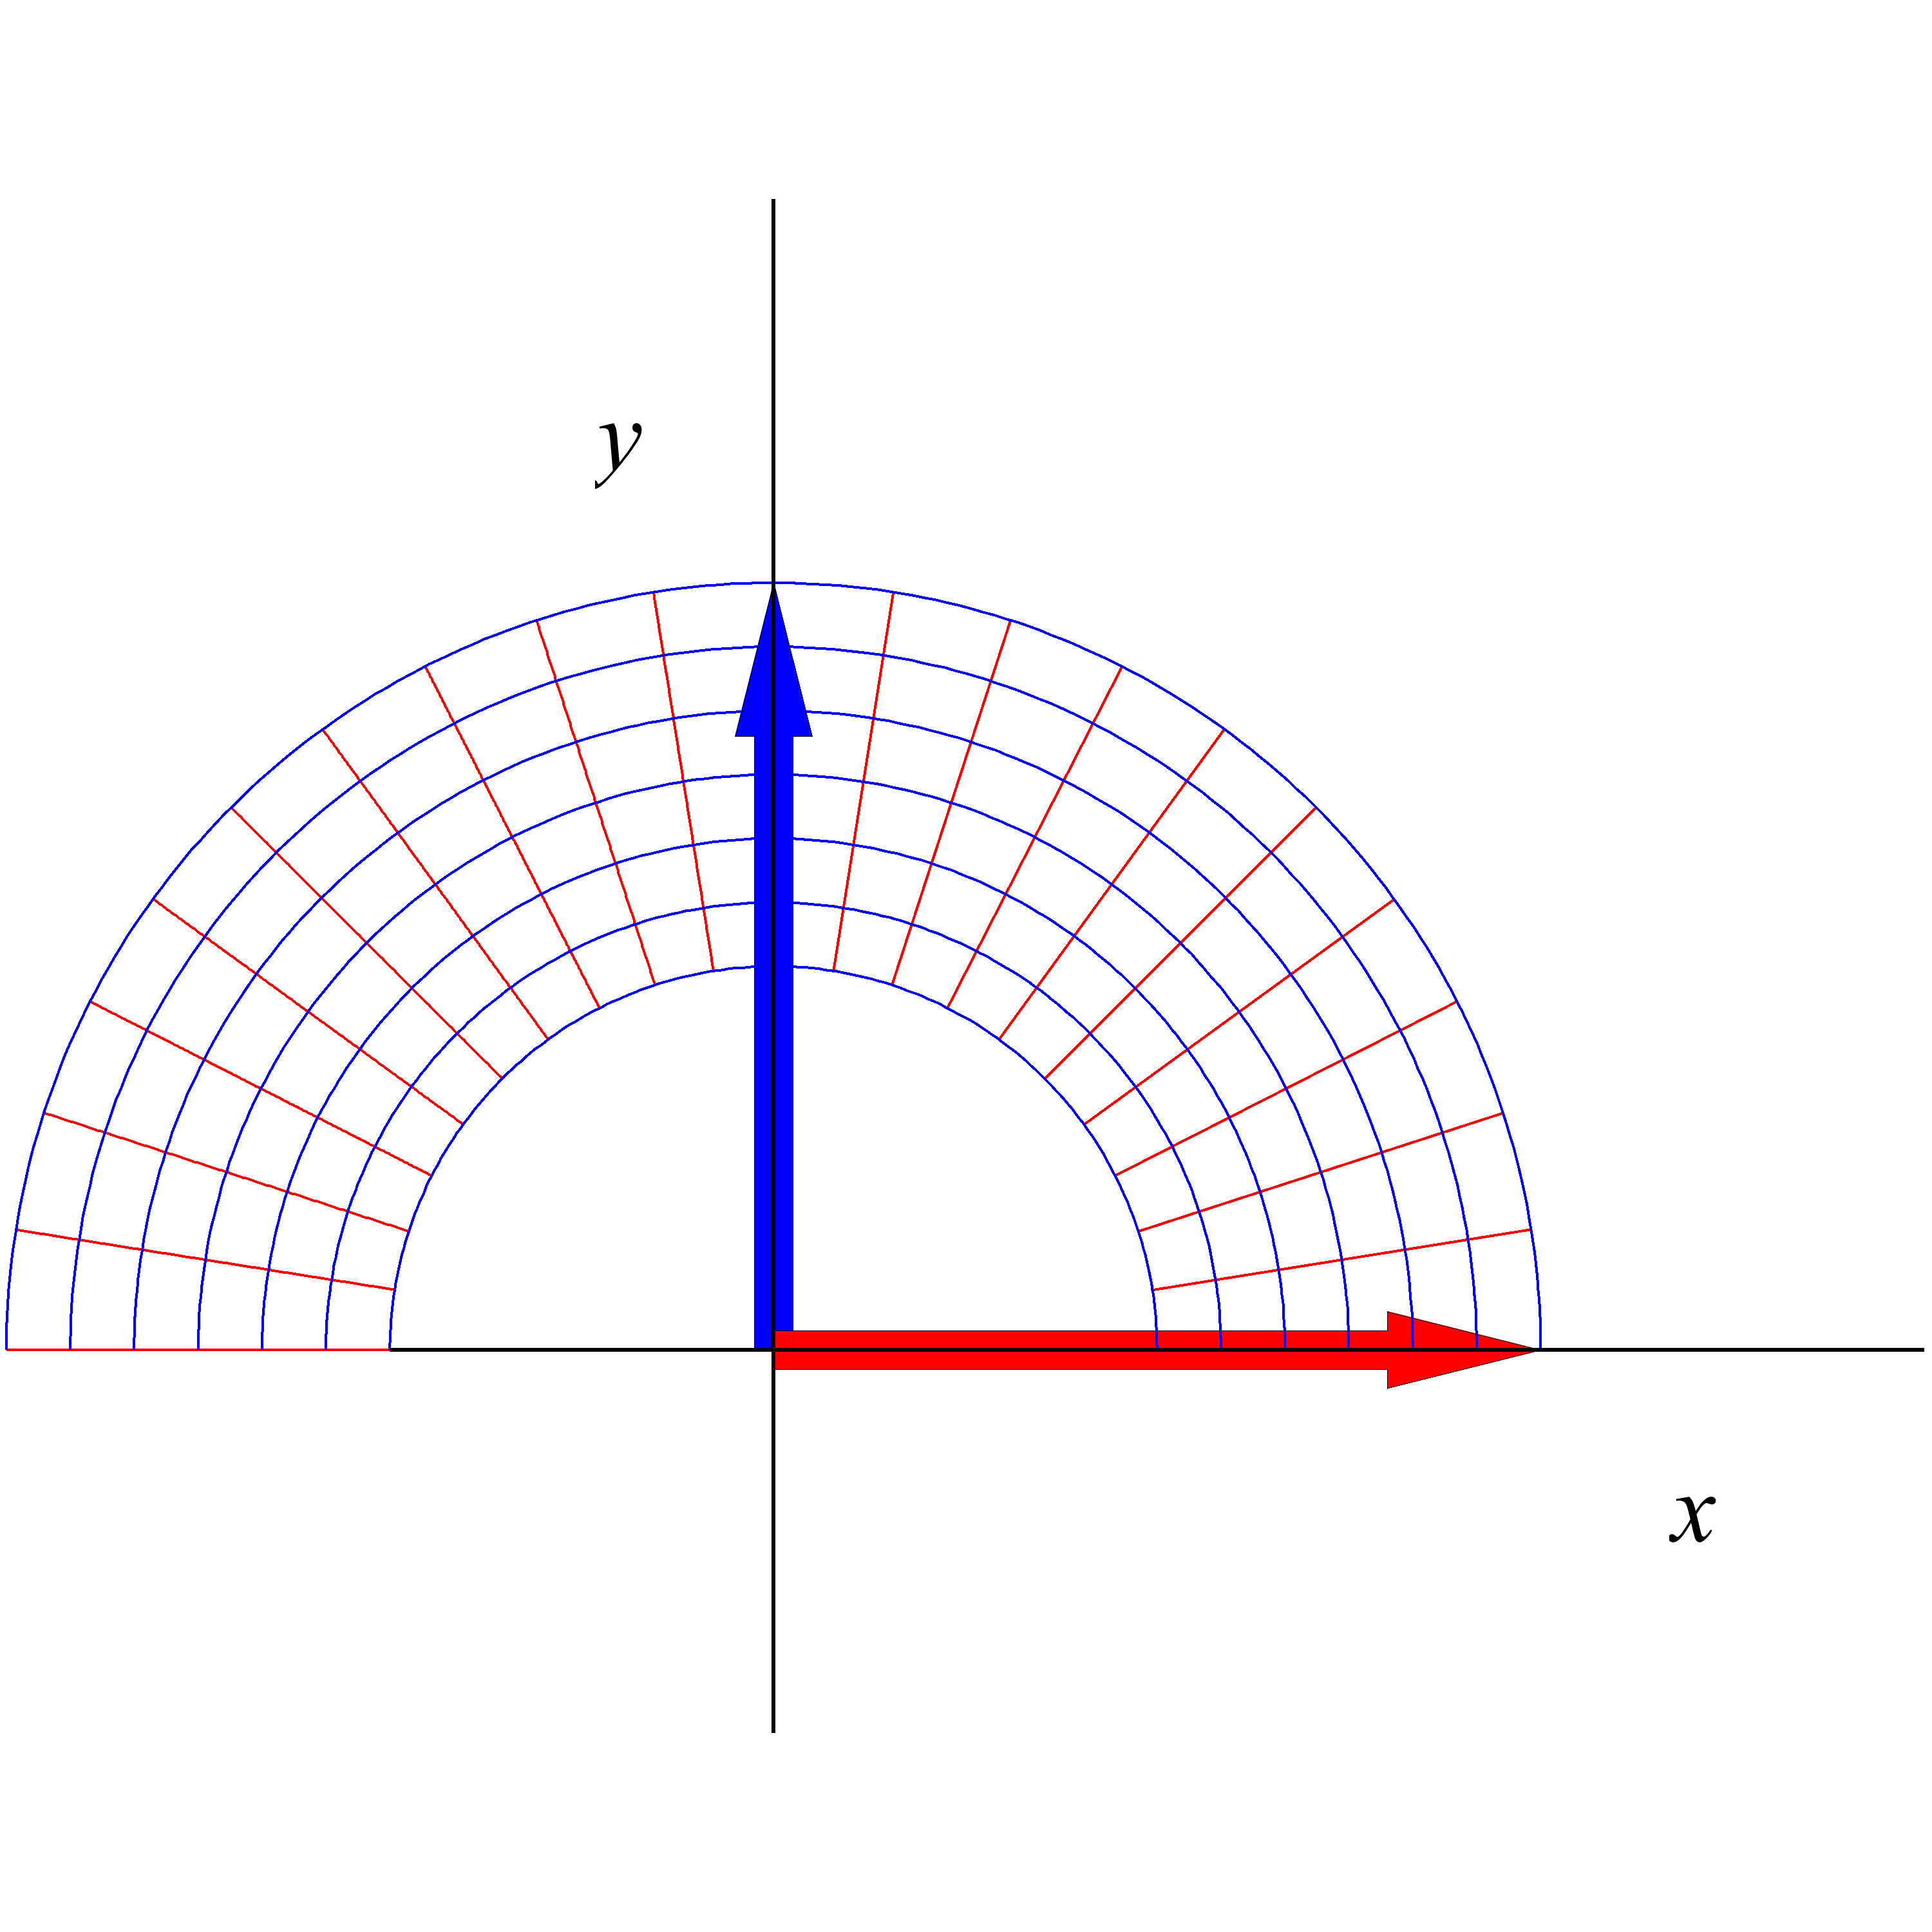
\includegraphics[height=60mm]{FIGS/plotAnnulusM2} 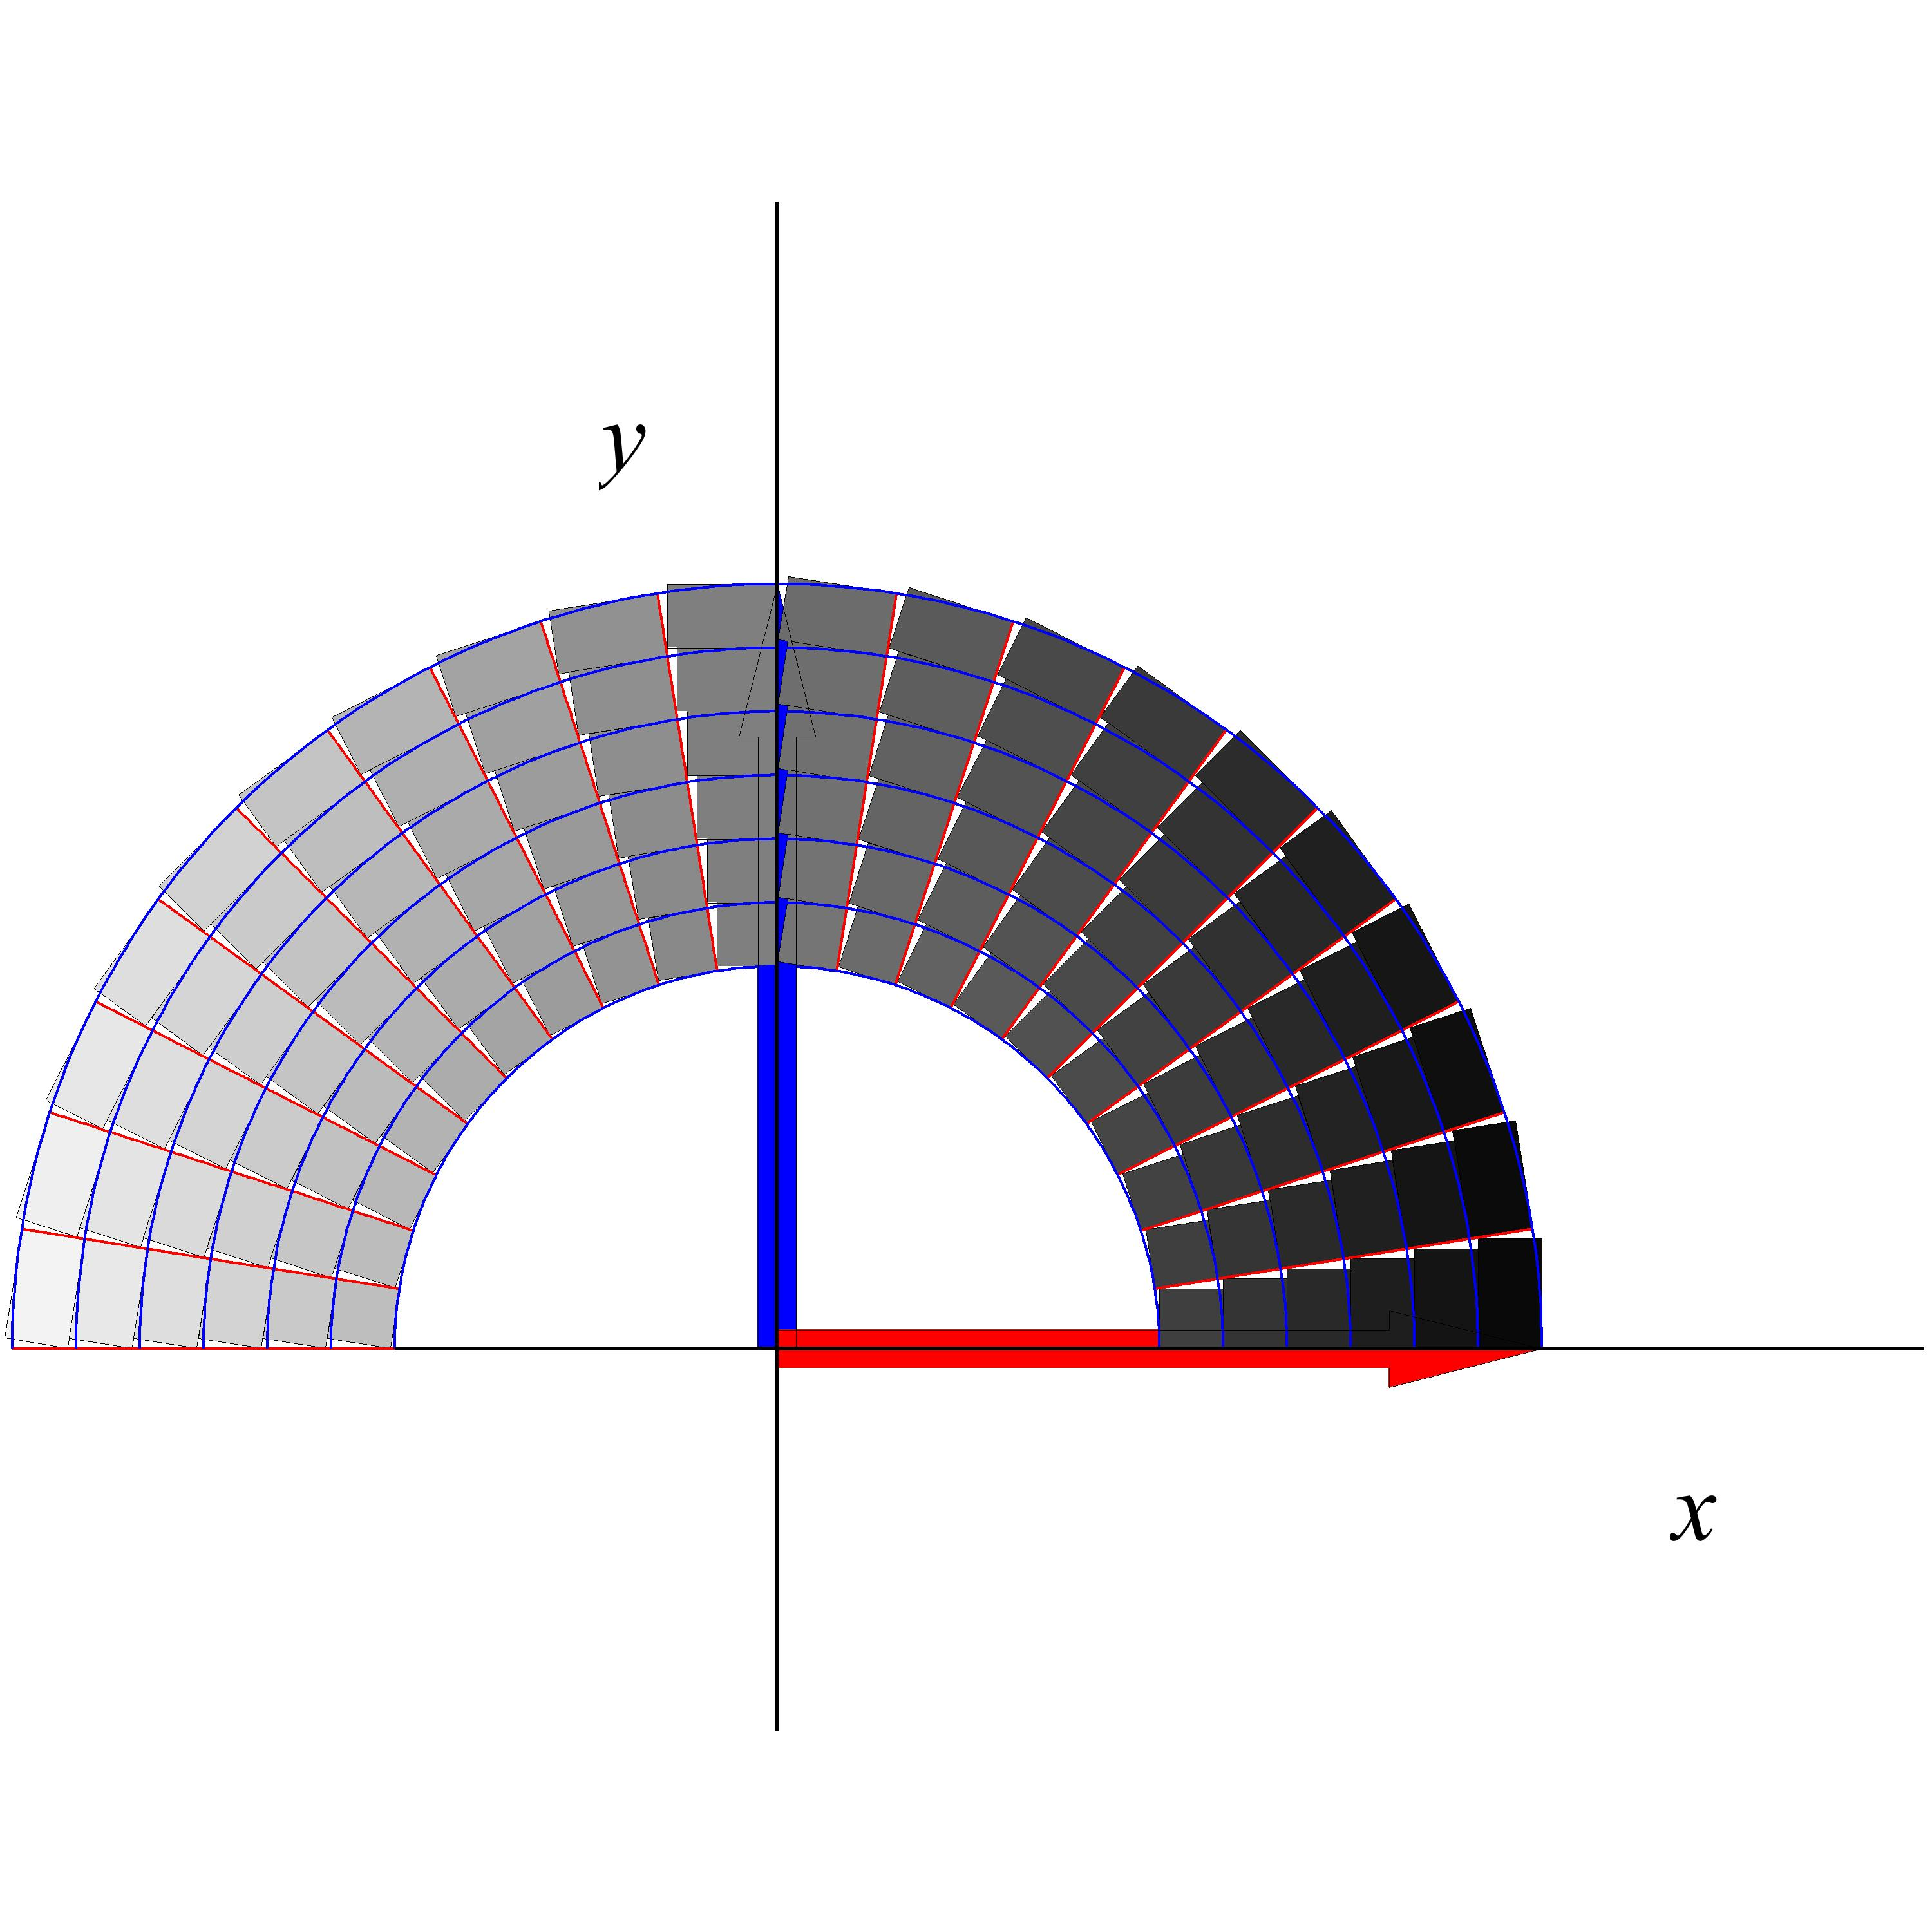
\includegraphics[height=60mm]{FIGS/plotAnnulusM3}}
\begin{center}
\caption{\small{Et (halvt) ring-område i planen med antydet vægtfordeling. Se
eksempel \ref{exampAnnulMass}. }} \label{figAnnulMass}
\end{center}
\end{figure}


%%%%%%%%%%%%%%%%%%%%%%%%%%%%%%%%%%%%%%%%%%%%%%%%%%%
%%%%%%%%%%%%%%%%%%%%%%%%%%%%%%%%%%%%%%%%%%%%%%%%%%%
%%%%%%%%%%%%%%%%%%%%%%%%%%%%%%%%%%%%%%%%%%%%%%%%%%%
%%%%%%%%%%%%%%%%%%%%%%%%%%%%%%%%%%%%%%%%%%%%%%%%%%%










%%%%%%%%%%%%%%%%%%%%%%%%%%%%%%%%%%%%%%%%%%%%%%%%%%%%%%%%%%%%%
%%%%%%%%%%%%%%%%%%%%%%%%%%%%%%%%%%%%%%%%%%%%%%%%%%%%%%%%%%%%%
%%%%%%%%%%%%%%%%%%%%%%%%%%%%%%%%%%%%%%%%%%%%%%%%%%%%%%%%%%%%%

\begin{summary}
Vi har i denne eNote opstillet de begreber og metoder, der giver os præcise
udtryk for længder af kurver, arealer af plane områder og mere generelt kurve- og plan-integraler af
(vægt-)funktioner på kurver og plane områder, der er parametriserede ud fra henholdsvis et interval
eller et rektangulært parameter-område. Kurve- og plan-integralerne er opstillet ved hjælp af de respektive Jacobi-funktioner, som angiver hvor meget para\-me\-ter\-inter\-val\-let eller parameter-området lokalt deformeres når det afbildes over i den ønskede kurve eller over i det ønskede plane område ved de valgte vektor-afbildninger $\mathbf{r}(u)$ og $\mathbf{r}(u, v)$.
\begin{itemize}
\item For en rum-kurve $K_{\bf r}$ med parameterfremstillingen $\mathbf{r}(u)= (x(u), y(u), z(u))$ har vi følgende motiverede kurveintegral af funktionen $f(x,y,z)$ over rumkurven:
\begin{equation}
\int_{K_{\bf r}} f \, d\mu \, = \, \int_{a}^{b} f({\bf
r}(u))\,\Jac_{\bf r}(u)\,du \quad ,
\end{equation}
hvor {Jacobi-funktionen $\Jac_{\bf r}(u)$} er givet ved længden af parametriseringens tangentvektor:
\begin{equation}
\Jac_{\bf r}(u) \, = \,  | {\bf r}'(u) | \quad .
\end{equation}

\item For et plant område $P_{\bf r}$  med parameterfremstillingen $\mathbf{r}(u,v)= (x(u,v), y(u,v))$ har vi ligeledes motiveret følgende definition af planintegralet af funktionen $f(x,y)$ over området:
\begin{equation} \label{eqPlanIntegral}
\int_{P_{\bf r}} f \, d\mu \, = \, \int_{c}^{d} \int_{a}^{b}
f({\bf r}(u,v))\, \Jac_{\bf r}(u,v)\,du \, dv \quad,
\end{equation}
hvor Jacobi-funktionen $\Jac_{\bf r}(u,v)$ nu er givet ved parallelogram-arealet udspændt af koordinatkurvernes tangentvektorer:
\begin{equation} \label{eqJacPlan}
 \Jac_{\bf r}(u,v)\, = \,
 | {\bf r}'_{u}(u,v) | \cdot | {\bf
r}'_{v}(u,v) | \cdot \sin(\theta(u,v)) \quad ,
\end{equation}
hvor $\theta(u,v) \in [0, \pi]$ betegner vinklen mellem de to tangentvektorer ${\bf r}'_{u}(u,v)$ og ${\bf r}'_{v}(u,v)$.
\end{itemize}
\end{summary}


%%%%%%%%%%%%%%%%%%%%%%%%%%%%%%%%%%%%%%%%%%%%%
%%%%%%%%%%%%%%%%%%%%%%%%%%%%%%%%%%%%%%%%%%%%%
%%% HER SKAL DU STOPPE MED AT SKRIVE %%%%%%%%
%%%%%%%%%%%%%%%%%%%%%%%%%%%%%%%%%%%%%%%%%%%%%
%%%%%%%%%%%%%%%%%%%%%%%%%%%%%%%%%%%%%%%%%%%%%


\end{document} 

%%%%%%%%%%%%%%%%%%%%%%%%%%%%%%%%%%%%%%%%%%%%%%%%%%%
%%%%%%%%%%%%%%%%%%%%%%%%%%%%%%%%%%%%%%%%%%%%%%%%%%%

